\documentclass[12pt]{article}
\usepackage{amsmath}
\usepackage{adjustbox}
\usepackage{tabularx}
\usepackage{graphicx}
\usepackage[a4paper,bindingoffset=0.2in,%
left=1in,right=1in,top=1.2in,bottom=1.2in,%
footskip=.25in]{geometry}
\usepackage{hyperref}
\hypersetup{
	colorlinks=true,
	linkcolor=blue,
	filecolor=blue,      
	urlcolor=blue,
	citecolor=blue
}
\usepackage{natbib}
\usepackage{rotating}
\usepackage{threeparttable}
\usepackage{caption}
\usepackage{subcaption}
	
%opening
\title{Rigidity of Expectations: Additional Evidence from Density Forecasts of Professionals and Households}
\author{Tao Wang}


\begin{document}
	
	\maketitle
	
	\begin{abstract}
		Surveys on density forecasts of macroeconomic variable that are not availables until recently provide one additional moment restriction, uncertainty, for testing and exploring the implications of various theories on expectation formation. This paper first documents the persistent dispersion in uncertainty about future inflation as well as other stylized facts across economists and households.  Second,  utilizing the panel data of individual uncertainty, I provide additional test results and estimates that are not consistent with the benchmark prediction of full-information rational expectation (FIRE). Finally, using externally identified shocks to inflation, I show the dynamic responses of forecasting moments to shocks are broadly consistent with theories of expectation rigidity and additional evidence for shock-dependent nature of the rigidity.  This sets the stage for estimating shock-specific rigidity using uncertainty as the next step of the analysis.  
		
	\end{abstract}
	
	\newpage 
	
	\section{Introduction}
	
	
	Theories on how agents form expectations in ways deviating from rational expectation(RE) have proliferated over the past decade. This has been also accompanied by an increasingly welcoming recognition of the use of surveys by macroeconomists in testing these theories empirically.  On one hand, various theories built upon different micro foundations produce somewhat similar macro patterns. For instance, the notion of expectation rigidity micro-founded by different theories mostly generate a sluggish response to new information.  On the other hand, there are important and subtle differences in testable predictions from these theories for both individual forecasts and aggregate moments of the forecasts. 
	
	This paper extends this research effort by bringing an additional moment of forecasts into perspective, i.e. uncertainty. Specifically, in this paper, I first derive the testable predictions from various theories on uncertainty and carefully compare the differences mostly obvious seen from uncertainty. Second empirically I test and estimate these implications utilizing the recently available probabilistic forecasts from both professional forecasters survey and household survey. Overall, the paper finds additional evidence from uncertainty consistent with the rigidity models. In the same time, the degree of rigidity appears to be shock-specific and bears the difference between households and professional forecasters. 
	
	The contributions of this paper primarily rely upon the additional insights from the forecast uncertainty, that is only available if surveyees are asked to assign their perceived probabilities to a range of values of the variable of forecast\footnote{For an insightful survey on the importance of measuring subjective expectations using probabilistic surveys, see \citet{manski2004measuring}.}. With density forecasts,  the variance of individual forecast can be estimated as an indicator of the uncertainty. Across different vintages of the forecast, the revision in uncertainty is a direct measure of  information gain or the degree of forecasting efficiency. Besides, the dispersion of uncertainty across agents, and its relationship with other moments widely examined by the literature, such as forecast errors and disagreements provide many insights as to how the agents expectation actually work.  
	
	This paper is related to three strands of literature. First, the recent decade has seen an emergence of the empirical work directly testing and evaluating the various theories on expectations theories using survey data. For instance, \citet{mankiw2003disagreement}, \citet{carroll2003macroeconomic}, \citet{branch2004theory}. More recent examples include \citet{coibion2018firms} on firms' managers. In addition to testing particular sets of theories, there is also a number of papers that show people's expectations are driven by idiosyncratic demographics, cognitive abilities and macroeconomic histories experienced(\citet{malmendier2015learning}, \citet{das2017socioeconomic} and \citet{d2019iq}, etc.). In terms of the methodology, this paper is closest to \citet{coibion2012can} and \citet{fuhrer2018intrinsic}.  However, all of these research simply rely upon point forecasts instead of density forecast or surveyed uncertainty. This is one theme on which this paper differs from the existing literature.   
	
	Second, the literature that has been originally developed under the theme of forecast efficiency provides a framework analyzing the dynamics of uncertainty useful for the purpose of this paper. The focus of the forecasting efficiency literature is evaluating forecasters' performance and improving forecasting methodology, but it can be adapted to test the theories of expectation formation of different types of agents. This is especially relevant to this paper as I focus on the uncertainty. 
	
	Third, \citet{manski2004measuring} and many other papers have advocated long for elicitating probabilistic questions measuring subjective uncertainty in economic surveys. Although the initial suspicion concerning to people's ability in understanding, using and answering probabilistic questions is understandable, \citet{bertrand2001people} and other work have all shown that this is actually less of a concern. \citet{armantier2017overview} have a thorough discussion on designing, experimenting and implementing the consumer expectation surveys to insure the quality of the responses. Broadly speaking, the advocators have argued that going beyond the revealed preference approach, availability to survey data provides economists with direct information on agents' expectations and helps avoids imposing arbitrary assumption.  This insight holds for not only point forecast, but also and even more importantly, for uncertainty.
	
	The paper is organized as followed. Section \ref{theory} first sets up a common framework in which testable various theories can be compared. Also, I derive the testable predictions from these theories for individual and population uncertainty as well as other moments. Section \ref{empirical} discusses the survey data used for this paper and presents both the stylized patterns and time series regressions that test the implications of these theories.   Section \ref{ShockBased} includes results from estimating the impulse response of forecast moments to externally identified shocks.  Section \ref{Conclusion} concludes the paper and discusses the plan for the next step. 
	
	\section{Theories of Expectation Formation}\label{theory}
	
	\subsection{Definition of moments}
	
	An agent $i$ is forming expectations about a stochastic variable $y^i_{t+h}$. The superscript $i$ can be dropped if it is an aggregate (i.e. inflation) variable instead of individual-specific  (i.e. household income or house value). This paper focuses on forecasting of aggregate variables, in particular, inflation. So we can simply denote the variable as $y_{t+h}$.  \footnote{Only in the context of aggregate variable, it make sense to study the population moments such as average expectations and disagreements. Studying expectations of idiosyncratic variables requires individual panel data, as well as the idiosyncratic realizations of the variable. }
	
	Denote $ f_{i,t+h|t}$ as agent i's $h$-period-ahead density forecast. $ f_{i,t+h|t}$ is the conditional density of $y_{i,t+h}$ given the information set $I_{i,t}$ available at time $t$. 
	
	$$f_{i,t+h|t} \equiv f_{i,t}(y_{t+h}|I_{i,t})$$
	
	
	$I_{i,t}$ is the information set available for individual $i$ at time t. The information set can be  agent specific, thus it has subscript $i$.  The specific content contained in $I_t$ varies from different models of expectation. For instance, sticky expectation and rational inattention literature all assume that agents are not able to update new information instantaneously. So the information set may not contain the most recent realization of the variable of forecast $y_t$. \footnote{Given the same information set available to agents, different theories may also differ in the underlying models each agent use to form the conditional density of the variables by agent $i$. For instance, \citet{patton2010forecasters} finds that the disagreements are driven by not only difference in information but also heterogeneity in prior and models. More theoretical work includes multi-prior or model uncertainty such as \citet{hansen2001robust}, \citet{hansen2008robustness}, etc.}
	
	Accordingly, h-period ahead mean forecast at $t$, denoted as $ y_{i,t+h|t}$, is the conditional expectation of $y_{t+h}$ by the agent $i$. 
	
	$$y_{i,t+h|t} \equiv E_{i,t}(y_{t+h}) =\int f_{i, t+h|t} d y_{t+h}$$
	
	Similarly, individual forecasting variance $\sigma_{i,t+h|t}$, hereafter termed as individual uncertainty in this paper, is the conditional variance.
	
	$$\sigma^2_{i,t+h|t} \equiv Var_{i,t}( y_{t+h} )$$
	
	Individual forecast error $FE_{i,t+h|t}$ is the difference of ex post realized value of $y_{t+h}$ and individual forecast at time $t$. 
	
	$$FE_{i,t+h|t} = y_{i,t+h|t} - y_{t+h}$$
	
	The population analogs of individual mean forecast, uncertainty and forecast errors are simply the average of the individual moments taken across agents. Denote them as $\bar y_{t+h|t}$, $\bar \sigma^2_{t+h|t}$, and $\overline{FE}_{t+h|t}$, respectively. Hereafter, they are termed as the population mean forecast, population uncertainty and population forecast error, respectively. In addition, disagreement is defined as the cross-sectional variance of mean forecasts of individual agents.  Denote it as $\overline{Var}_{t+h|t}(y_{i,t+h|t}) $. To simplify notation, let us directly call it $\overline{Disg}_{t+h|t}$.  
	
	To abuse the language, I refer to the 3 individual indicators and 4 population indicators as moments and they are  listed in Table \ref{MomSum} 
	
	\begin{table}[ht]
		\centering
		\caption{Definition and Notation of Moments}
		\label{MomSum}
		\begin{tabular}{ll}
			
			\hline 
			Individual Moments                                  & Population Moments                             \\
			\hline 
			Mean forecast: $y_{i,t+h|t}$                   & Average forecast: $\bar y_{t+h|t}$                   \\
			Forecast error: $FE_{i,t+h|t}$ & Average forecast error: $\overline{FE}_{t+h|t}$ \\
			Uncertainty: $\sigma^2_{i,t+h|t}$         & Average uncertainty:  $\bar \sigma^2_{t+h|t}$ \\
			& Disagreements:  $\overline{Disg}_{t+h|t}$       \\
			\hline 
		\end{tabular}
	\end{table}
	
	Finally, we assume the underlying true process of $y_{t}$ is $AR(1)$ with persistence parameter $0<\rho <1$ and i.i.d. shock $\omega_t$. 
	
	\begin{eqnarray}\label{AR_process}
		y_{t} = \rho y_{t-1} + \omega_t
	\end{eqnarray}
	
	$$\omega_t \sim N(0,\sigma^2_{\omega})$$
	
	Although we make the assumption of i.i.d. shock, the framework allows for the possibility of time-varying volatility, i.e. the variance of $\omega_t$ is thus $\sigma^2_{t,\omega}$ with time subscript. 
	
	\subsection{Benchmark of full-information rational expectation(FIRE)}
	
	In the FIRE benchmark,  it is assumed that all agents perfectly observe $y_t$ at time $t$ and understand the true process of $y$. Therefore, the individual forecast is $\rho^h y_t $, which is shared by all agents. Therefore, it is also equal to the average forecast. 
	
	Both individual and population forecast errors are simply the realized shocks between $t+1$ to $t+h$.  
	
	\begin{eqnarray}\label{NoPastInfFE}
		\overline{FE}^{*}_{i,t+h|t} = \sum^{h}_{k=1} \rho^k \omega_{t+k}
	\end{eqnarray}
	
	I use superscript of $*$ to denote all the moments according to FIRE. It is easy to see that the forecast error is orthogonal to information available till time $t$. This provides the a well known null hypothesis of FIRE.
	
	The second implication from FIRE here is that forecast errors of non-overlapping horizon are not correlated. (Equation \ref{NoSerialCorrFE}). For instance, forecast error at time $t$ and that at time $t+h$ or further are not serially correlated. This is not the case within $h$ periods as the realized shocks in overlapping periods enter both forecast errors.  These FE-based restrictions of FIRE provide the foundations for the tests used in Table \ref{NullTest}. 
	
	\begin{eqnarray}\label{NoSerialCorrFE}
		Cov(\overline{FE}^{*}_{t+h|t}, \overline{FE}^{*}_{t+s+h|t+s}) = 0 \quad \forall s \geq h
	\end{eqnarray}
	
	Concerning uncertainty, the first simple implication by FIRE is that all individual shares the same degree of uncertainty. The uncertainty about future $y$ simply comes from uncertainty about unrealized shocks between $t$ and $t+h$. With the same model in mind (Equation \ref{AR_process}) and the same information $y_t$, everyone's uncertainty is equal to the weighted sum of the future volatility before its realization. (Equation \ref{VarREIndPop}). In FIRE, there are neither disagreements about mean, nor disagreements about the uncertainty \footnote{This is the same to \citet{jurado2015measuring}'s terminology.} 
	
	\begin{eqnarray}\label{VarREIndPop}
		\bar \sigma^{*2}_{t+h|t} = \sum^{h}_{s=1}\rho^{2s} \sigma^2_{\omega}
	\end{eqnarray}
	
	The time series behavior of h-year-ahead uncertainty, i.e. $\sigma^2_{t+h|t}$, $\sigma^2_{t+h+1|t+1}$, etc, depends on the true process of $y$. Specifically, it depends if $\sigma^2_\omega$ is time-varying. If time-invariant, h-period-ahead uncertainty is simply as constant. In baseline case, I make such an assumption, in general it may not be true. \footnote{For example, \citet{justiniano2008time}, \citet{vavra2013inflation} on time-varying volatility of inflation.} 
	
	The testable implication of rationality lies in the revision of uncertainty. Hereafter, we refer revision (instead of change) as the difference of moments across vintages of forecast with the fixed terminate date of realization. For instance, the difference between the uncertainty about $y_{t+h}$ at time $t$ and the uncertainty about $y_{t+h}$ at time $t-1$.
	
	More generally,  denote the forecast of $y_{t+h}$ over the horizon of $h-k$ as $y_{t+h|t+k} \quad \forall k =0,1...h$. Then the uncertainty at different points of the $k$ is the following. 
	
	\begin{eqnarray}\label{VarREPop}
		\bar \sigma^{*2}_{t+h|t+k} = \sum^{h-k}_{s=1}\rho^{2s} \sigma^2_{\omega}
	\end{eqnarray}
	
	As the forecaster approaches $t+h$ ($k$ approaches to $h$), there is an unambiguous reduction in uncertainty (or efficiency gain in the forecasting literature) as more and more shocks have realized. Equivalently, revision is always negative and should be exactly equal to the variance of the realized shocks according to FIRE. 
	
	Moving from $t$ to $t+1$, for instance, revision in uncertainty can be also expressed as a function of the previous revision.  
	
	\begin{eqnarray}\label{VarREPopRv}
		\begin{aligned}
			\bar \sigma^{*2}_{t+h|t+1} - \bar \sigma^{*2}_{t+h|t} & = - \rho^{2h}\sigma^2_\omega \\
			& =  \rho (\bar \sigma^{*2}_{t+h|t} - \bar \sigma^{*2}_{t+h|t-1})
		\end{aligned}
	\end{eqnarray}
	
	Lastly, FIRE has predictions about disagreements. As agents perfect update the same information, there is no disagreements at any point of the time. 
	
	\begin{eqnarray}\label{DisgREPop}
		\overline{Disg}^{*}_{t+h|t}=0 \quad \forall t
	\end{eqnarray}
	
	Another simple result is that both disagreements and uncertainty do not respond to realized shocks any any point of the time. But this does not differentiate FIRE from other models. 
	
	\subsection{Sticky Expectation (SE)}
	
	The theory of sticky expectation (\citet{mankiw2002sticky}, \citet{carroll2003macroeconomic} etc.), regardless of various micro-foundations, builds upon the assumption that agents do not update information instantaneously as they do in FIRE. One tractable assumption is that there is a homogenous Poisson rate $\lambda$ of updating among the population. Specifically, at any point of time $t$, each agent learns about the up-to-date realization of $y_t$ with the probability of $\lambda$; otherwise, it forms the expectation based on the most recent up-to-date realization of $y_{t-\tau}$, where $\tau$ is the time experienced since the last update. 
	
	Denote the mean forecast of a non-updater since $t-\tau$ as $y_{i,t+h|t-\tau}$ since her forecast conditions upon the information up till $t-\tau$. 
	
	\begin{eqnarray} 
		y_{i,t+h|t-\tau} = \rho^{h+\tau} y_{t-\tau}
	\end{eqnarray}
	
	Now her information set is not up to date, the uncertainty to a non-updater is higher than an updater and it increases with the duration of non-updating $\tau$. 
	
	\begin{eqnarray}\label{VarSEInd}
		\sigma^2_{i,t|t-\tau}= \sum^{h+\tau}_{s=1}\rho^{2s} \sigma^2_{\omega}
	\end{eqnarray}	
	
	In FIRE, updating at each period $t$ resolves only the uncertainty about the shocks that have just realized in $t$. In contrast, in SE each updating resolves the uncertainty about all the realized shocks since the last update. From $t-\tau$ to $t$, the revision in uncertainty is 
	
	\begin{eqnarray}
		\sigma^2_{i,t+1|t} - \sigma^2_{i,t+1|t-\tau} = \rho^{2} \sigma^2_{\omega} - \sum^{\tau+1}_{s=1}\rho^{2s} \sigma^2_{\omega} = -\sum^{\tau+1}_{s=2} \rho^{2s}\sigma^2_{\omega}
	\end{eqnarray}
	
	FIRE basically assumes  $\tau=1$ for all the agents and all the time, namely all agents' last update takes place in the previous period. So setting $\tau =1$ in the above equation gives the reduction in uncertainty in FIRE. The reduction in uncertainty is greater in SE for any $\tau>1$ than FIRE.
	
	In the individual level, the key difference between FIRE and SE is that the later does not reduce uncertainty  as efficiently as in the former primarily because of the rigidity incorporating new information. In the same time, note that the rigidity in updating according to SE cannot be systematically observable in the individual level, both in terms of forecasts errors and uncertainty. This is because the behaviors of each individual forecast specifically depend on if she updates or not in that period. 
	
	Relying upon the law of large numbers, one can derive testable predictions about population moments that allow us perform tests of sticky expectation and recover rigidity parameter $\lambda$. \footnote{\citet{carroll2003macroeconomic} is good example of this for households.} 
	
	One well known prediction from SE is that the average forecast is a weighted average of update-to-date rational expectation and lagged average expectation as reproduced below. \footnote{See \citet{coibion2012can} or appendix of this paper for detailed steps.} It can be also expressed as a weighted average to all the past realizations of $y$. Setting $\lambda=1$, then the SE collapses to FIRE and the average forecast is equal to $y$'s long-run mean of zero.
	
	\begin{eqnarray}\label{MeanSEPop}
		\begin{aligned}
			\bar y_{t+h|t} & = \lambda \underbrace{y^*_{t+h|t}}_{\textrm{rational expectation at t}} + (1-\lambda) \underbrace{\bar y_{t+h|t-1}}_{\textrm{average forecast at } t-1} \\
			& = \lambda \sum^{\infty}_{\tau=0} (1-\lambda)^\tau y^*_{t+h|t-\tau} \\
			& = \lambda \sum^{\infty}_{\tau=0} (1-\lambda)^\tau \rho^{h+\tau}y_{t-\tau}
		\end{aligned}
	\end{eqnarray}
	
	It is easy to show that the average forecast errors are serially correlated(Equation \ref{FESEPop}). For double checking, setting $\lambda=1$, SE collapses to FIRE, in which there is no serial correlation between forecast errors and it fully responds to newly realized shocks at time $t$.  
	
	\begin{eqnarray}\label{FESEPop}
		\begin{aligned}
			\overline{FE}_{t+h|t}  = (1-\lambda) \overline {FE}_{t+h|t-1} + \lambda \rho^h \omega_t 
		\end{aligned}
	\end{eqnarray}
	
	Similarly, the inefficiency of reducing uncertainty in SE takes the following form in the aggregate level. Average uncertainty at any point of time is now a weighted average of uncertainty to agents whose last updates have taken place in different periods of past. 
	
	
	\begin{eqnarray}\label{VarSEPop}
		\begin{aligned}
			\bar \sigma^2_{t+h|t} & = \sum^{+\infty}_{\tau =0} \underbrace{\lambda (1-\lambda)^\tau}_{\text{fraction of non-updater until }t-\tau} \underbrace{\sigma^2_{t+h|t-\tau}}_{\text{ uncertainty of most recent update at }t-\tau} \\
			& = \sum^{+\infty}_{\tau =0} \lambda (1-\lambda)^\tau \sum^{h+\tau}_{s=0}\rho^{2s} \sigma^2_{\omega}
		\end{aligned}
	\end{eqnarray}
	
	
	Since not all agents incorporate the recently realized shocks, the revision in average uncertainty exhibits serial correlation described in Equation \ref{VarSERv}. It is a weighted average of the resolution of uncertainty from the most recent shocks and its lagged counterpart. 
	
	\begin{eqnarray}\label{VarSERv}
		\begin{aligned}
			\bar \sigma^2_{t+h|t+1} - \bar \sigma^2_{t+h|t} = (1-\lambda)(
			\bar \sigma^2_{t+h|t} - \bar \sigma^2_{t+h|t-1}) -\lambda \rho^{2h} \sigma^2 
		\end{aligned}
	\end{eqnarray}
	
	In particular, the second component is the information gain from the most recent realization of the shock underweighted by $\lambda<1$. The first component is the inefficiency sourced from the stickiness of updating. The higher rigidity (lower $\lambda$), the smaller the efficiency gain or uncertainty reduction compared to in FIRE. 
	
	Lastly, SE also predicts non-zero disagreements and sluggish adjustment compared to FIRE. This is because of different lags in updating across populations. 
	
	\begin{eqnarray}\label{DisgSEPop}
		\begin{aligned}
			\overline{Disg}_{t+h|t} & = \lambda \sum^{\infty}_{\tau=0} (1-\lambda)^{\tau} (y_{t+h|t-\tau} - \bar y_{t+h|t }))^2  
		\end{aligned}
	\end{eqnarray}
	
	From time $t$ to $t+1$, the change in disagreements comes from two sources. One is newly realized shock at time $t+1$. The other component is from people who did not update at time $t$ and update at time $t+1$.  
	
	\citet{coibion2012can} derive the impulse response of dispersion at time $t+k$ to a shock that realized at $t$. Disagreements rise after realization of the shock and gradually returns to its steady state level.  
	
	\begin{eqnarray}
		\rho^{2(h+k)} (1-\lambda^{k+1})\lambda^{k+1} \omega^2_t
	\end{eqnarray}
	
	
	
	\subsubsection{Summary of predictions of SE}
	
	\begin{itemize}
		\item Population mean forecast partially responds to shocks and with lags. 
		\item Forecast errors are serially correlated. 
		\item Population disagreements rise in response to new shocks and return to steady state level gradually. 
		\item Population average uncertainty revision under-reacts volatility of the shocks.
	\end{itemize}
	
	\subsection{Noisy information(NI)}
	
	A class of models (\citet{lucas1972expectations}, \citet{sims2003implications}, \cite{woodford2001imperfect}, etc.), noisy information(NI) hereafter, describes the expectation formation as a process of extracting or filtering true variable $y_t$ from a sequence of realized signals.  The starting assumption is that the agent cannot observe the true variable perfectly. Unlike SE, it is assumed that agents keep track of the realizations of signals instantaneously all the time. 
	
	We assume agent $i$ observe two signals $s^{pb}$ and $s^{pr}_i$, with $s^{pb}$ being public signal common to all agents, and $s^{pr}_i$ private signals being individual specific with subscript $i$. The generating process of two signals are assumed to be the following.
	
	\begin{eqnarray}\label{NISigDef}
		\begin{aligned}
			s^{pb}_t = y_t + \epsilon_t, \quad \epsilon_t \sim N(0,\sigma^2_\epsilon)\\ 
			s^{pr}_{i,t} = y_t + \xi_{i,t} \quad \xi_{i,t} \sim N(0,\sigma^2_\epsilon)
		\end{aligned}
	\end{eqnarray}
	
	Stacking the two signals into one vector $s_{i,t} = [s^{pb}_t,s^{pr}_{i,t}]'$ and $v_{i,t}= [\epsilon_t,\xi_{i,t}]'$, the equations above can be rewritten as 
	
	\begin{eqnarray}
		\begin{aligned}
			s_{i,t} = H y_{t} + v_{i,t} \\
			\text{where } & H=[1,1]' \quad \\
		\end{aligned}
	\end{eqnarray}
	
	
	Now any agent trying to forecast future $y$ has to form her expectation of the contemporaneous $y$. Denote it as  $y_{i,t|t}$, which needs to be inferred from the signals to agent $i$. The agent's best h-period ahead forecast is simply iterated $h$ periods forward based on the AR(1) process and it is equal to $\rho^h y_{i,t|t}$. This is the same as FIRE.
	
	What is different from FIRE is that the agent makes her best guess of $y_t$ using Kalman filtering at time $t$. Specifically, the mean forecast of individual $i$ is the posterior mean based on her prior and realized signals $s_{i,t}$. 
	
	
	\begin{eqnarray}
		\begin{aligned}
			y_{i,t|t}  
			& =  \underbrace{y_{i,t|t-1}}_{\text{prior}} + P \underbrace {(s_{i,t|t}-s_{i,t|t-1})}_{\text{innovations to signals}} \\
			& = (1-PH) y_{t|t-1} + Ps_{i,t} \\
			& = (1-PH) y_{t|t-1} + PH y_{t} + P v_{i,t} 
		\end{aligned}
	\end{eqnarray}
	
	where the Kalman gain $P$ is a vector of size of two that determines the degrees of reaction to signals. 
	
	
	\begin{eqnarray}
		\begin{aligned}
			P = [P_\epsilon,P_\xi]= \Sigma^y_{i,t|t-1} H(H'\Sigma^y_{i,t|t-1} H + \Sigma^v)^{-1} 
		\end{aligned}
	\end{eqnarray}
	
	$\Sigma^y_{i,t|t-1}$  is the variance of  $y_t$ based on prior belief. Here the capital case of $\sigma$ is used to be consistent with vector operations. 
	
	\begin{eqnarray}
		\begin{aligned}
			\Sigma^v =  \left[ \begin{matrix} 
				\sigma^2_{\epsilon} &  0 \\ 
				0 & \sigma^2_\xi \end{matrix}\right] 
		\end{aligned}
	\end{eqnarray}
	
	Individual forecast partially responds to new signals as  $PH<1$. $PH=1$ is a special case when both signals are perfect thus $\Sigma^v = 0$, then the formula collapses to FIRE. 
	
	
	A comparable parameter with $1-\lambda$ in SE that governs rigidity in NI is $1-PH$. It is a function of previous period uncertainty about $y_t$ and noisiness of the signals determined by $\Sigma^v$. Note $P$ is time variant as the variance is updated by the agent each period. The time varying nature of rigidity will be discussed later. For now, I drop time $t$ from $P$ to avoid clustering.  
	
	The under-reaction to news generate serial correlation of forecast errors with the coefficient being $\rho^2(1-PH)$. it does not only depend on $PH$, but also the forecast horizon $h$. As $\rho<1$, the rigidity declines with a longer horizon. In this regard, the rigidities implied by NI and SE are different because the form is fixed and the later is horizon dependent. 
	
	What differentiates average forecast from individual's is the role played by private signals. On average, private signals cancel out across agents, therefore, only public signals enter the average forecast, thus, average forecast errors (Equation \ref{FENIPop}). 
	
	\begin{eqnarray}\label{FENIPop}
		\begin{aligned}
			\bar y_{t+h|t} & = \rho^h [(1-PH) \underbrace{\bar  y_{t+h|t-1}}_{\text{Average prior}} + P \underbrace{\bar s_{t}}_{\text{Average Signals}}] \\
			& = (1-PH) \bar y_{t+h|t-1}+ P [\epsilon_t, 0]' \\
			& = (1-PH) \bar y_{t+h|t-1} + P \epsilon_t
		\end{aligned}
	\end{eqnarray}
	
	Kalman filtering also updates the variance according to the rule of normal updating.   The posterior variance at time $t$ is a linear function of uncertainty in the previous period and variance of signals. 
	
	\begin{eqnarray}
		\begin{aligned}
			\Sigma^y_{i,t|t} = \Sigma^y_{i,t|t-1} - \Sigma^y_{i,t|t-1} H'(H \Sigma^y_{i,t-1} H' +\Sigma^v) H \Sigma^y_{i,t|t-1} 
		\end{aligned}
	\end{eqnarray}
	
	This directly gives the revision in uncertainty from time $t-1$ to $t$. The newly arrived information, although noisy, still brings about information gains, thus leading to an unambiguously drop on uncertainty. But due to the signal is not perfect, i.e. $\Sigma^v \neq 0$, there is inefficiency in reducing uncertainty compared to FIRE. 
	
	\begin{eqnarray}\label{VarNIRv}
		\Sigma^y_{i,t|t} - \Sigma^y_{i,t|t-1} = - \Sigma^y_{i,t|t-1} H'(H \Sigma^y_{i,t-1} H' +\Sigma^v) H \Sigma^y_{i,t|t-1} <0
	\end{eqnarray}
	
	In order to be directly comparable with the revision in uncertainty in FIRE (Equation \ref{VarREPopRv}) and SE (Equation \ref{VarSERv}), the nowcasting uncertainty about $y_t$ needs to be converted to $h$-period-ahead forecasting uncertainty. This is simply to add the nowcasting uncertainty discounted by $\rho^{2h}$ to the uncertainty about future unrealized shocks.   
	
	\begin{eqnarray}\label{VarNIEq}
		\Sigma_{i,t+h|t} = \rho^{2h} \Sigma_{i,t|t} + \sum^{h}_{s=1}\rho^{2s} \sigma^2_{\omega}
	\end{eqnarray}
	
	As a result, the revision in h-period-ahead uncertainty from $t-1$ to $t$ only partially reacts to the resolution of  uncertainty from newly realized shock $\omega_t$ in the past period. 
	
	Assuming the nosiness of the private signal is equal across agents, then the dynamic of population uncertainty is the same to individual counterpart $\bar \Sigma_{t+h|t}$, since in NI, every agent is faced with the same filtering problem.  
	
	Figure \ref{IllustrateNI} illustrates the Kalman filtering problem over the $10$-period horizon from to $t$ to $t+10$  following a one-time shock of one standard deviation of $\omega_t$.  For illustration purpose, I assume that both private and public signals have an equal degree of noisiness and their standard deviation is equal to the unconditional standard deviation of $y$, i.e. $\sqrt{\frac{\sigma^2_\omega}{1-\rho^2}}$.  A particular draw of public and private signals from their respective conditional distributions given $y_t$ are plotted.    
	
	From the top left figure, the agent's nowcasting $y_{t+k|t+k}$, namely her best real-time guess based on prior and the realized signal at each period roughly tracks the $y_{t+k}$ and responds partially to signals in each period. Correspondingly, her forecasting of $y$ at $t+10$ also centers around the true value. 
	
	FIRE implies agent learns realized $y$ in each period perfectly. Thus the nowcasting remains zero throughout the whole horizon. Nowcasting uncertainty picks up in the realization of shock and gradually declines as more and more information signals are realized. This comes from the information gains from Kalman filtering. 
	
	In the first sight, the sharp rise in nowcasting uncertainty at the beginning of the period being only humbly reflected in the forecasting uncertainty seems counterintuitive. Actually this is due to nowcasting uncertainty is discounted by the factor of $\rho^2(h-k)$.  (Equation \ref{VarNIEq}). It is also interesting that for the particular configurations of the noisiness of the signals, the drop in forecasting uncertainty from NI is not as inefficient as one may have expected compared to FIRE.  This has important quantitative implications for NI models. In particular, the nosiness of the signals needs to be consistent with the degree of rigidity. I will return this point in the next section.  
	
	\begin{figure}[ht]
		\centering
		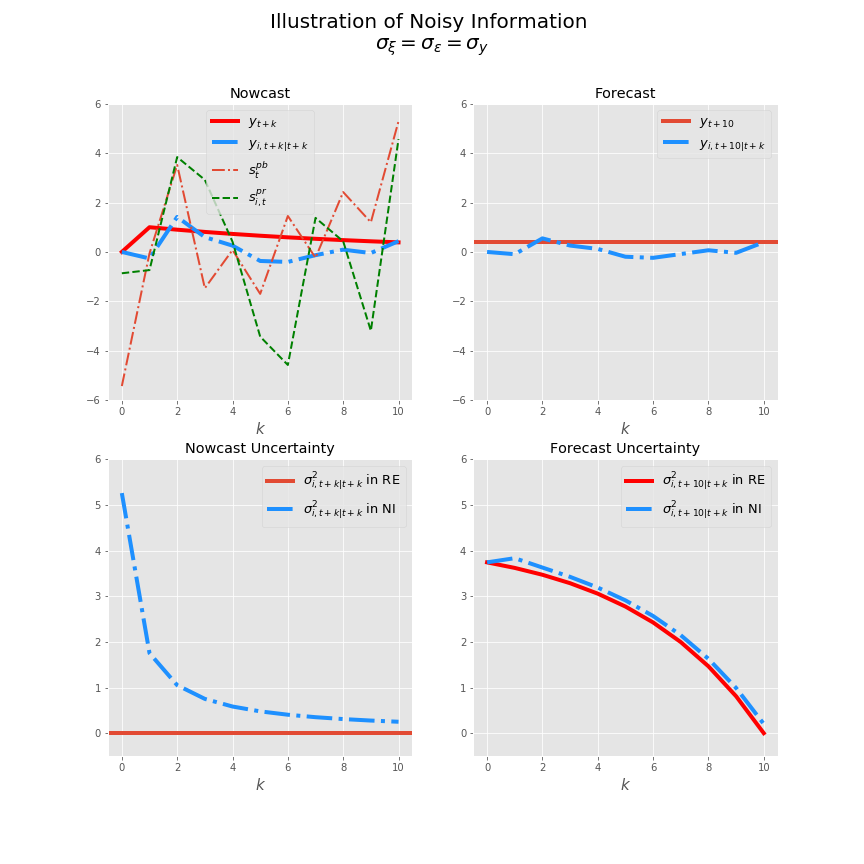
\includegraphics[width=13cm]{figures/ni_illustration.png}  \\
		\begin{flushleft}
		{\footnotesize Note: the top two figures plot the nowcasting of $y_{t+k}$  at time $t+k$ and forecasting of $y_{t+h}$ at time $t+k$  based on a Kalman filtering together with FIRE after a one-time shock of one unit at time $t$. The nowcasting and forecasting uncertainty are correspondingly plotted in the bottom. Both private signal and public signal have the conditional variance equal to long-run variance of y, i.e.  $\sigma_\epsilon = \sigma_\xi = \sigma_y$. The plotted signals are are a pair of particular draw from their respective conditional distribution. }
		\end{flushleft}
		\caption{Nowcasting and Forecasting in Noisy Information}
		\label{IllustrateNI}
	\end{figure}
	
	NI also predicts non-zero disagreement in the presence of private signals. The behavior of disagreement across agents come from the difference in realized private signals. Specifically, it is equal to the following. 
	
	\begin{eqnarray}
		\begin{aligned}
			\overline {Disg}_{t+h|t} = \rho^{2h} P^2_\xi \sigma^2_\xi  
		\end{aligned}
	\end{eqnarray}
	
	The implications for disagreement are straightforward. First, the disagreement decrease with the forecast horizon for the reason of discounting. Second, the disagreement depends on noisiness private signals, but not on that of public signals and the variance of the true variable $y$. Third, similar to SE, the disagreements also increase with the rigidity parameter $P$ in this model.
	
	\subsubsection{Summary of predictions from noisy information}
	
	\begin{itemize}
		\item Individual and population expectation adjusts in each period, but only partially adjusts to new information. 
		\item  Individual and population uncertainty unambiguously drop each period as one approaches the period of realization.  
		\item  Population disagreements rise in each period as time approaches the period of realization. Disagreements will never be zero. 
	\end{itemize}
	
	
	\subsection{Comparing FIRE, SE and NI}
	
	Taking stock, both SE and NI predict rigidity in incorporating the arrival of new information. In the former context, the rigidity comes from the simple non-updating of the most realization of the variable. In the latter case, the rigidity comes from a partial reaction to new information due to the nosiness of the signals.  In addition to forecast and disagreements, the rigidity is also reflected in the dynamics of uncertainty.  Uncertainty in SE does not resolve as rapidly as in FIRE because the newly realized shocks do not get updated by some of the agents. While in NI, the drop in uncertainty is dampened because there is additional uncertainty associated with the real-time realization of the variable.  
	
	Figure \ref{ir_pop} illustrates the impulse response of population moments to a hypothetical one-time shock of size one unit at time $t$ according to different theories. Still, I maintain the assumption in \ref{IllustrateNI} that the standard deviation of private and public signals are both equal to one unconditional standard deviation of $y$.  And the $\lambda$ is set to be $0.75$, implying on average an update interval of four quarters.  
	
	
	Both FE and disagreements from SE and NI exhibit sluggish adjustment following the shock as we have anticipated. Both pick up in the time of the shock and gradually declines over the horizon as the forecaster approaches terminate date $t+10$. The difference is that in NI, both the forecast and forecast errors move up and downs around the smooth version of the SE since signals are not perfect. 
	
	The dynamic of disagreements and uncertainty, however,  illustrate one parametric difference between SE and NI. In particular,  the initial increase in disagreements is higher for NI compared to SE for the particular parameter values. This implies that the noise of the private signal that drives the disagreements in NI exceeds that the extent to which the agents do not simultaneously update in SE. \footnote{Another subtle point is that if the disagreements jump the highest in the time of the shock turns out depend on value of $\lambda$. In the fixed horizon forecasting, $\lambda=0.5$ is the maximizer of disagreements.}
	
	For the same parameters, however, the inefficiency seen in dynamics of uncertainty seems to be much more substantial for SE than in NI. Overall, the uncertainty drops almost as efficiently as in FIRE. The difference between SE and the FIRE benchmark is more notable. This is the graphical illustration of Equation \ref{VarSERv}. 
	
	
	\begin{figure}[ht]
		\centering
		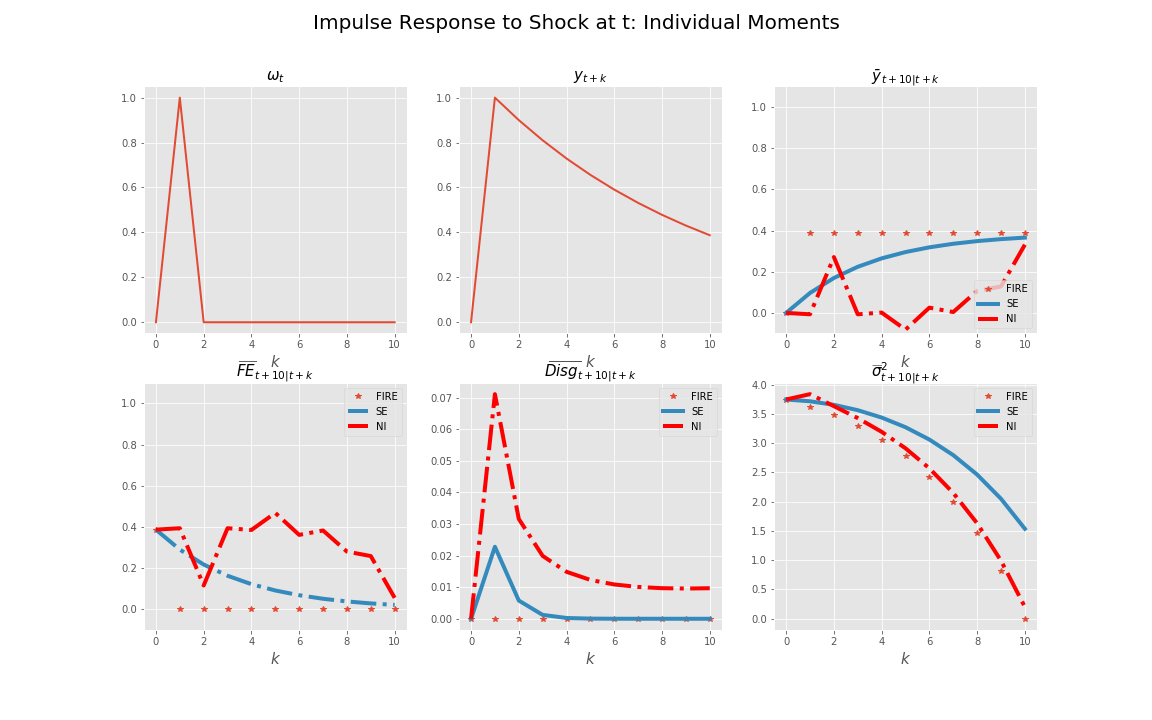
\includegraphics[width=\textwidth]{figures/ir_popseni.png} 
		\begin{flushleft}
			{\footnotesize Note: figure 1-6 plot the dynamics of a one-time shock to inflation $\omega_{t+k}$, the realized value of $y_{t+k}$,  average forecast of $\bar y_{t+10|t+k}$, forecasting errors $\overline{FE}_{t+10|t+k}$, disagreements $\overline {Disg}_{t+10|t+k}$, and uncertainty $\bar \sigma^2_{t+10|t+k}$ to a one-time shock  of unit one at time $t$, i.e. $\omega_t=1$. For NI, public and private signals’ variance is equal to long-run variance of $y$, i.e. $\sigma_\epsilon = \sigma_\xi = \sigma_\xi $. For SE, $\lambda = 0.25$.  }
		\end{flushleft}
		\caption{Impulse responses of population moments to a shock to inflation}
		\label{ir_pop}
	\end{figure}
	
	
	
	In order to understand why the rigidity seen from uncertainty is de facto much lower in NI that in SE for a sensible values of the noisiness of signals , I plot the implied rigidity from two models in Figure \ref{rigidity} for three different values of nosiness of signals in NI while fixing rigidity in SE to be $1-\lambda =0.75$. In particular, the noisiness range from $0.1$, $1$ and $10$ times of the long-run variance of $y$. 
	
	As it is made clear by the Figure, one notable difference between the two models is that SE's rigidity is exogenously fixed while NI's rigidity is endogenously determined by the horizon thus time varying. In particular, the implied rigidity from NI in the time of the shock, given there is substantial information gain from Kalman filtering in the same period, is quite low. For a noisiness of both signals as 10 times as high of the unconditional standard deviation of $y$, the rigidity only reaches the fixed rigidity in SE till the 8-th period. But since by that time, the initial information provided by the shock at time $t$ has been mostly absorbed by NI agent, so in fact the uncertainty revision in NI is quite efficient compared to SE models.  This echoes our earlier observation in Figure \ref{IllustrateNI}. 
	
	
	\begin{figure}[ht]
		\centering
		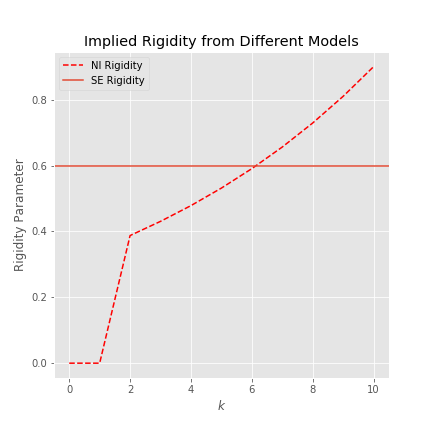
\includegraphics[width=0.7\textwidth]{figures/rigidity.png} 
		\begin{flushleft}
			{\footnotesize Note: implied rigidity is $1-\lambda$ in SE and $(1-P_{t+k}H)$ in NI. Rigidity from NI are plotted for three values of noisiness of signals, i.e. 0.1, 1 and 10 times of the unconditional variance of $y$. }
		\end{flushleft}
		\caption{Rigidity from Two Models}
		\label{rigidity}
	\end{figure}
	
	In summary, although NI and SE both predict the similar qualitative predictions of rigidity when it comes the behavior of FE and disagreements, de facto, the efficiency of forecasting from NI is higher than SE. The only additional uncertainty in NI to that in FIRE is the nowcasting uncertainty, which is discounted in future. While in SE, the uncertainty do come from the lagged update of information, which involve uncertainties about all the shocks that are not yet updated in agents' information set. 
	
	\section{Empirical Results}\label{empirical}
	
	\subsection{Data}
	
	The focus of this paper naturally restricts my options of the survey data to use compared to other empirical  literature of testing theories of expectation formation.  The surveys who have elicited density forecasts of macroeconomic variables for a sufficiently long period has been rare. Rarer, for the purpose of the paper, is the data structure that allows for comparing the revisions across vintages that have a fixed terminate date of realization, either in individual level or aggregate level. 
	
	Survey of Professional Forecasters(SPF) meet both criteria thanks to the density forecasts of a number of macroeconomic variables, including headline CPI and PCE inflation they have started eliciting since 2007. In particular, the density forecasts are both made for current year forecast, basically nowcasting, as well as one-year-ahead forecast. This allows for directly testing the implications from the revisions in uncertainty.  
	
	The New York Fed Survey of Consumer Expectation(SCE) that started in 2013 has at least met the first criteria. In particular, households are asked to provide their perceived probabilities to 1-year-ahead inflation for a range of values. \footnote{Most importantly, they are kindly reminded that all the probabilities need to add up to one. NY Fed stuff has excluded those who do not meet this criteria.} The high-frequency monthly panel structure also provides an invaluable chance to explore the dynamics of uncertainty. Around one third of the households are surveyed for 12 months.  
	
	I follow \citet{engelberg2009comparing} to estimate the density distribution of each individual surveyee for SPF. \footnote{Answers with positive probabilities assigned to three bins is fit with a generalized beta distribution. Depending on if there is open-ended bin on either side with positive probability, 2-parameters or 4-parameters of the beta distribution are estimated. For those with only two bins with positive probabilities and adjacent, it is fit with a triangular distribution. For only one bin with probability, a uniform distribution over the positive probability bin is fit. See my online appendix for the detailed steps of estimation of python codes.} This is the same approach adopted by the New York Fed researchers \citet{armantier2017overview} for SCE and directly provided their estimate of uncertainty. I directly use them. 
	
	Unsurprisingly, both surveys need some  winsorization. For SPF, I drop the outliers of mean forecast and uncertainty estimates at both top and bottom one percentile as these are typically abnormals that are due to measurement errors or other reasons.   For SCE, I drop top and bottom 5 percentile of mean forecasts and uncertainty as households mean forecast are inclined to give extreme values. All the results in this paper are robust to a different threshold such as 10 and 1 percentile. \footnote{For mean forecasts and uncertainty, respectively, this means dropping 6528 and 5096 observations, out of 68887 observations in total.}
	
	A summary of the data information is in Table \ref{DataInfo}. 

	\begin{table}[ht]
		\caption{Information of Data}
		\label{DataInfo}
		\begin{tabularx}{\textwidth}{|X|X|X|}
			\hline 
			& SCE & SPF        \\
			\hline 
			Time period                                    & 2013-2019                           &
			 2007-2019             \\
			 \hline 
			Frequency                                      & Monthly                                 & Quarterly                \\
			\hline 
			Sample Size                                    & 1,300                                   & 30-50                    \\
			\hline 
			Var in Density                       & 1-yr and 2-yr-ahead inflation          & 1-yr-ahead GDP deflator, Core CPI and Core PCE         \\
			\hline 
			Panel Structure                               & stay up to 12 months                    & average stay for 5 years \\
			\hline 
			Individual Info                        & Education, Income, Age, Location        & Industry    \\
			\hline 
		\end{tabularx}
	\end{table}
	
	Throughout the paper, I use three measures of inflation: headline CPI, core CPI and core PCE . Depending on the specific variable of forecast in the survey series, the realization of the corresponding inflation is used to compute moments such as forecast errors. Specifically, SPF has density forecasts for both core CPI and core PCE \footnote{SPF also  has density forecasts for GDP deflator(for GNP prior to 1992:Q1) going back to 1968. Since the ranges of the values as we as the definition have not been consistent over time. I do not use it in this paper.}. For SCE, as the households responders are asked about the overall inflation, It is the most appropriate to be interpreted as  headline CPI inflation. To simplify the expression, from now on, core CPI and core PCE are simply referred to as CPI and PCE, respectively. 

	\subsection{Stylized facts}
	
	Although the sheer magnitudes of the differences between professionals' moments and those of households are so big that a direct comparison of the two seems redundant, their respective within-agent-type correlation serves a ready checking device of some statistical consistency. Figure \ref{UnceratitnyOtherMoments} plots the population uncertainty against realized inflation,  forecast errors and disagreements in the first, second and third rows, respectively. 
	
	It is widely documented in literature \footnote{The list literature showing positive inflation and uncertainty is long. For example \citet{ball1990inflation}. } and resonated by anecdotal narratives that high inflation is typically associated with high inflation uncertainty. However, the observable correlation of realized inflation and the directly estimated average uncertainty from both professionals and households are at most weakly positive during the period between 2007-2019. In particular, the correlation coefficients  0.14, 0.12 and -0.24 for SPF's CPI forecast, SPF's PCE forecast and SCE's CPI expectation. This may suggest that during a period of persistently low and stable inflation, the conventional positive redux of inflation and uncertainty is not a good description of the relation of the two. 
	
	The middle row of Figure \ref{UnceratitnyOtherMoments} looks into the relationship between size of the forecast error and uncertainty. Although according to our benchmark framework in \ref{theory}, there is no mathematical correlation between the size of the forecast errors and uncertainty as the former depends on the realized shocks and the later depends on the volatility of the shock, it is worth checking if in the data a greater ex ante uncertainty implies bigger ex post forecast errors. The correlation coefficients of the two are -0.19, -0.18 and 0.27 for SPF CPI forecasts, SPF PCE forecasts and SCE's forecasts, respectively. The two indicators turn out to be negatively correlated for professional forecasts. Only households forecasts exhibit such a positive correlation.   
	
	The last row of Figure \ref{UnceratitnyOtherMoments} examines the relationship between disagreement and uncertainty. Many empirical literatures in macroeconomics use disagreements and uncertainty as if they are similar concepts. Such a confusion in practice is partly due to the difficulty of finding appropriate measures of uncertainty in the first place. But as we have presented in \ref{theory}, the two are concepts with distinct statistical definitions. The empirical pattern of the two,  as shown in the plots, also confirms that the two are different objects. The correlation coefficients of the two turn out to be negative, -0.31 and -0.37 for SPF forecasts. In stark contrast, households seem to bear a strong correlation of 0.43 between the two moments.  
	
	Overall, professional forecasters' moments exhibit patterns more consistency from a statistical point of view.  In contrast, the positive correlation across households' ex ante uncertainty, ex post forecast errors, and cross-section disagreements cannot be easily reconciled by the framework we set up in Section \ref{theory}. 
	
	Persistent disagreement in expectations has been used as an important stylized evidence inconsistent with the assumption of identical expectation embedded in FIRE, for instance, \citet{mankiw2003disagreement}. A similar fact-checking can be done with respect to individual uncertainty. FIRE predicts individual share an equal degree of uncertainty as  seen in Equation \ref{VarREPop}. In contrast, SE predicts that uncertainty of individuals differ in that agents are not equally updated at a point of the time (Equation \ref{VarSEInd}). NI allows for the possibility of homogeneity in uncertainty only under the stringent conditions of an equal precision of signals and the same prior of uncertainty (Equation \ref{VarNIEq}). Therefore, the presence of dispersion of uncertainty across agents can be read against FIRE.  
	
	Figure \ref{IQR_Unceratitny} plots the median inflation expectation along with its 25/75 percentiles in the left and its counterpart in uncertainty in the right column.  Not only there is long-lasting dispersion in individual forecasts, i.e. disagreement, but also notable heterogeneity in uncertainty across agents.  And not surprisingly, the dispersion of both forecasts and uncertainty of households are both of a much greater magnitude than that of the professionals. The 25/75 inter-quantile-range of households point forecasts is 4-5 percentage points compared to 1 percentage point of professionals. And the IQR of the uncertainty of households is around 150-200 times(12-14 times for standard deviation) as that of professional forecasters.  
	
	Besides, in terms of the distribution of uncertainty, there are households/professional difference and similarity. Households' uncertainty is more skewed toward to the right (higher uncertainty), meaning there is a wide dispersion in the high values of uncertainty. This can be also seen in Figure \ref{Unceratitny_Histogram}, where I plot the kernel density estimated distribution of uncertainty by year on. What is common for both types of agents is that the dispersion in uncertainty is persistent over time and do not show much time-variation.  
	
	Another pattern worth discussing in Figure \ref{IQR_Unceratitny} is that there is a notable rise in the dispersion of professional forecasts in the recent 2-3 years, primarily driven by an increase of upper side of the forecast (i.e. 75 percentile forecast increases from 1\% to 2\%). \footnote{This should be interpreted with caution since the disagreements of SPF forecasts shown in bottom row of Figure \ref{UnceratitnyOtherMoments} actually exhibits a gradual decline. } This is consistent with the observation in the top left two graphs of Figure \ref{Unceratitny_Histogram} that the distribution of inflation forecasts in recent years have become flattened.
	
	FIRE also predicts an unambiguous reduction in uncertainty as one approaches the date of realization, where the drop is exactly equal to the volatility of the realized shocks. Although quantitatively it is hard to check this, one can look if the distribution of the uncertainty revision concentrate in the negative range. Figure \ref{RevisionHist} plots the average revision in mean forecasts and uncertainty from 1-year-ahead forecast in year $t-1$ to the current-year nowcast in year $t$. The more negative range in which the revision lies, the more ``rational'' of the forecast. Looking from the histograms, uncertainty revision shows left-skewness relative to zero. This implies on average,  forecasters feel more certain for her nowcasts relative to her forecast made one year before.  Unfortunately, since SCE does not provide the data structure for this purpose, I cannot make a comparison between two types of agents. A formal test of revision equal to zero or being negative will be carried out in the Section \ref{NullTest}. 
	
	
	\begin{figure}[ht]
		\centering
		\begin{subfigure}[b]{\textwidth}
			\centering
			\caption{Realized Inflation and Uncertainty}
			\label{InfVar}
			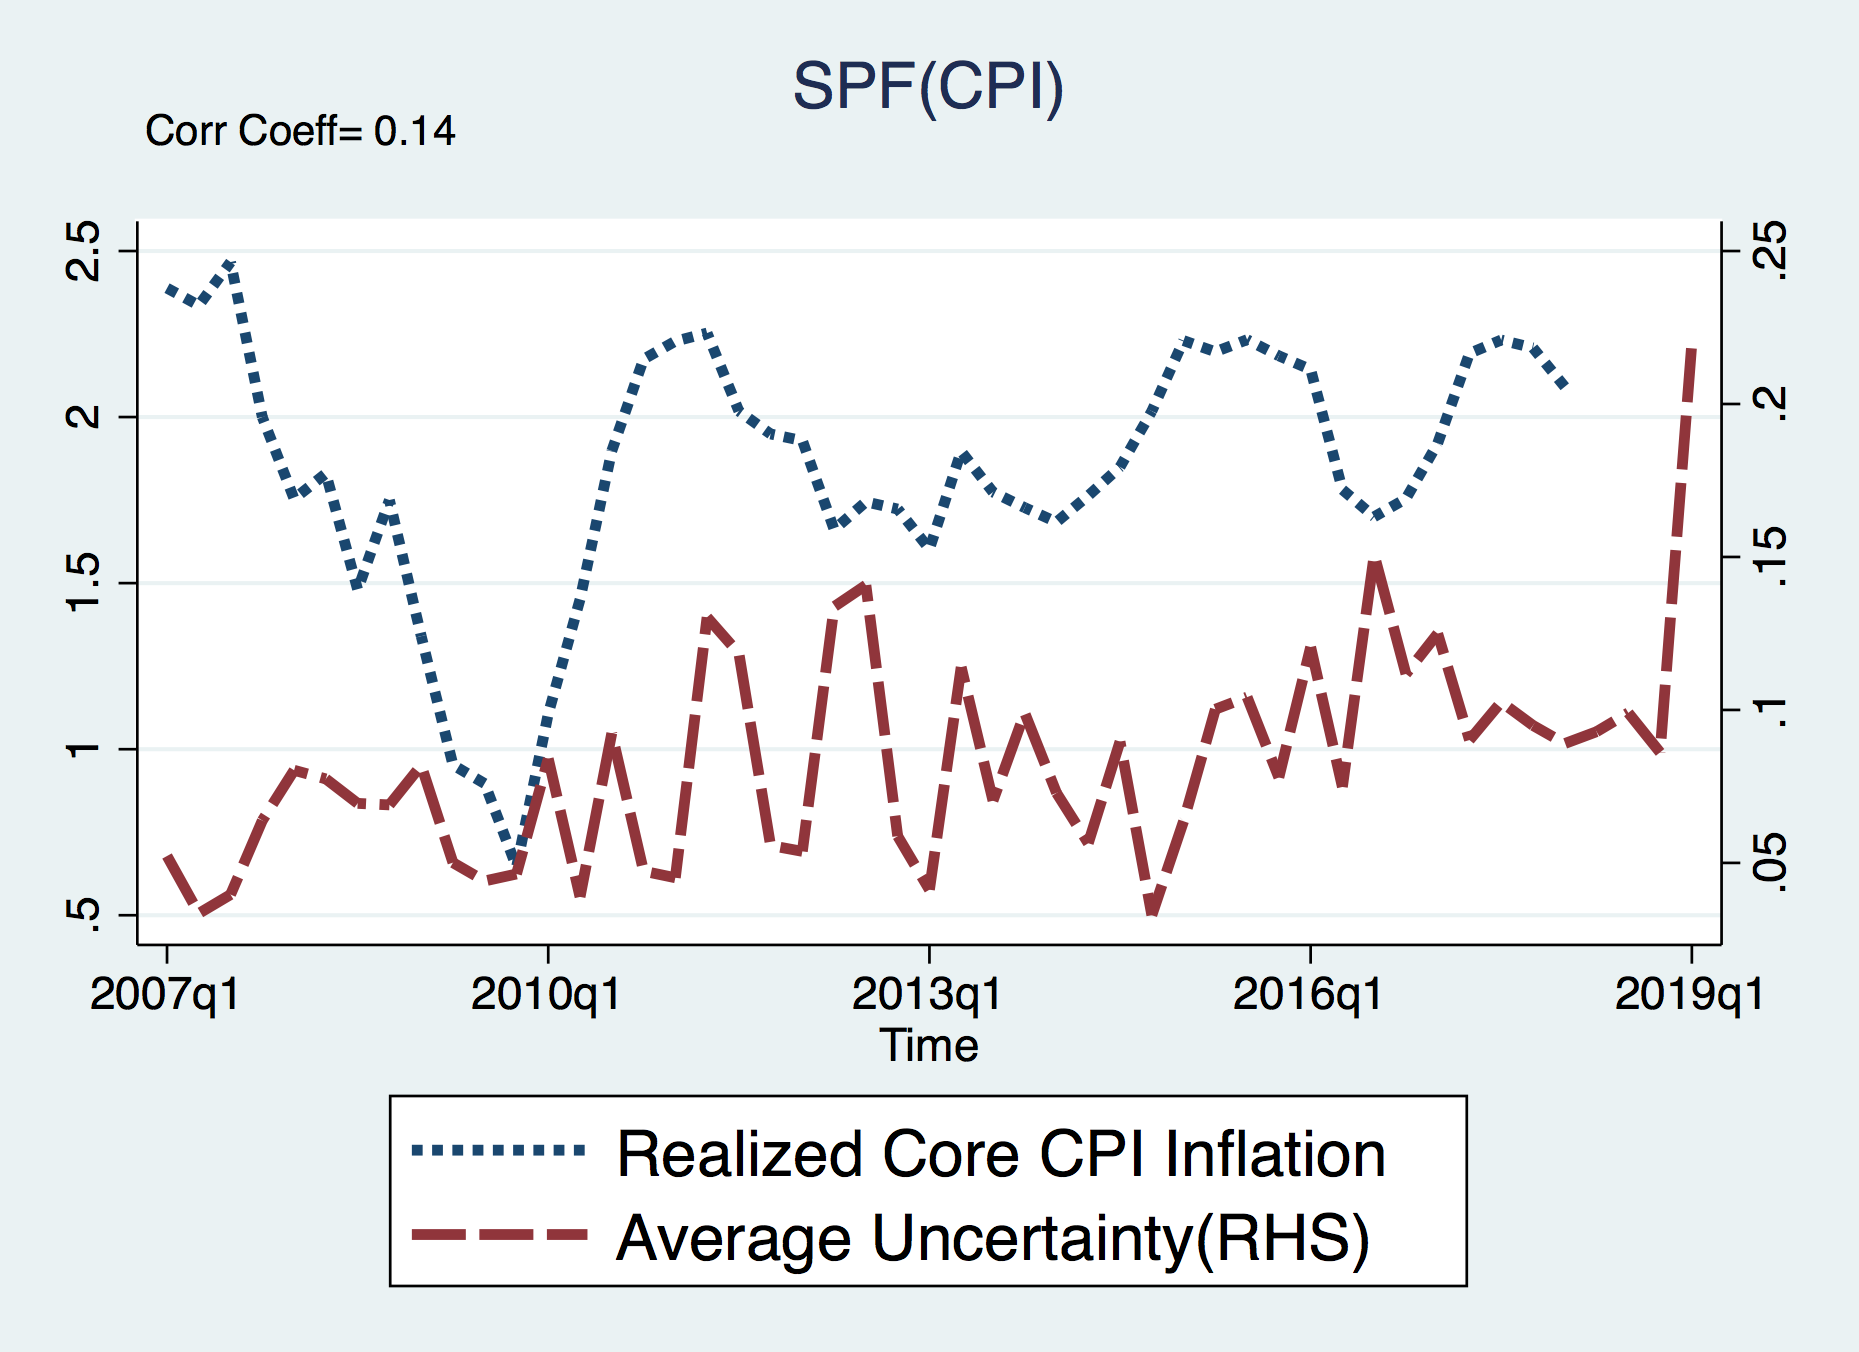
\includegraphics[width=0.3\textwidth]{figures/Inf1yf_CPICore_varSPFCPIQ.png}
			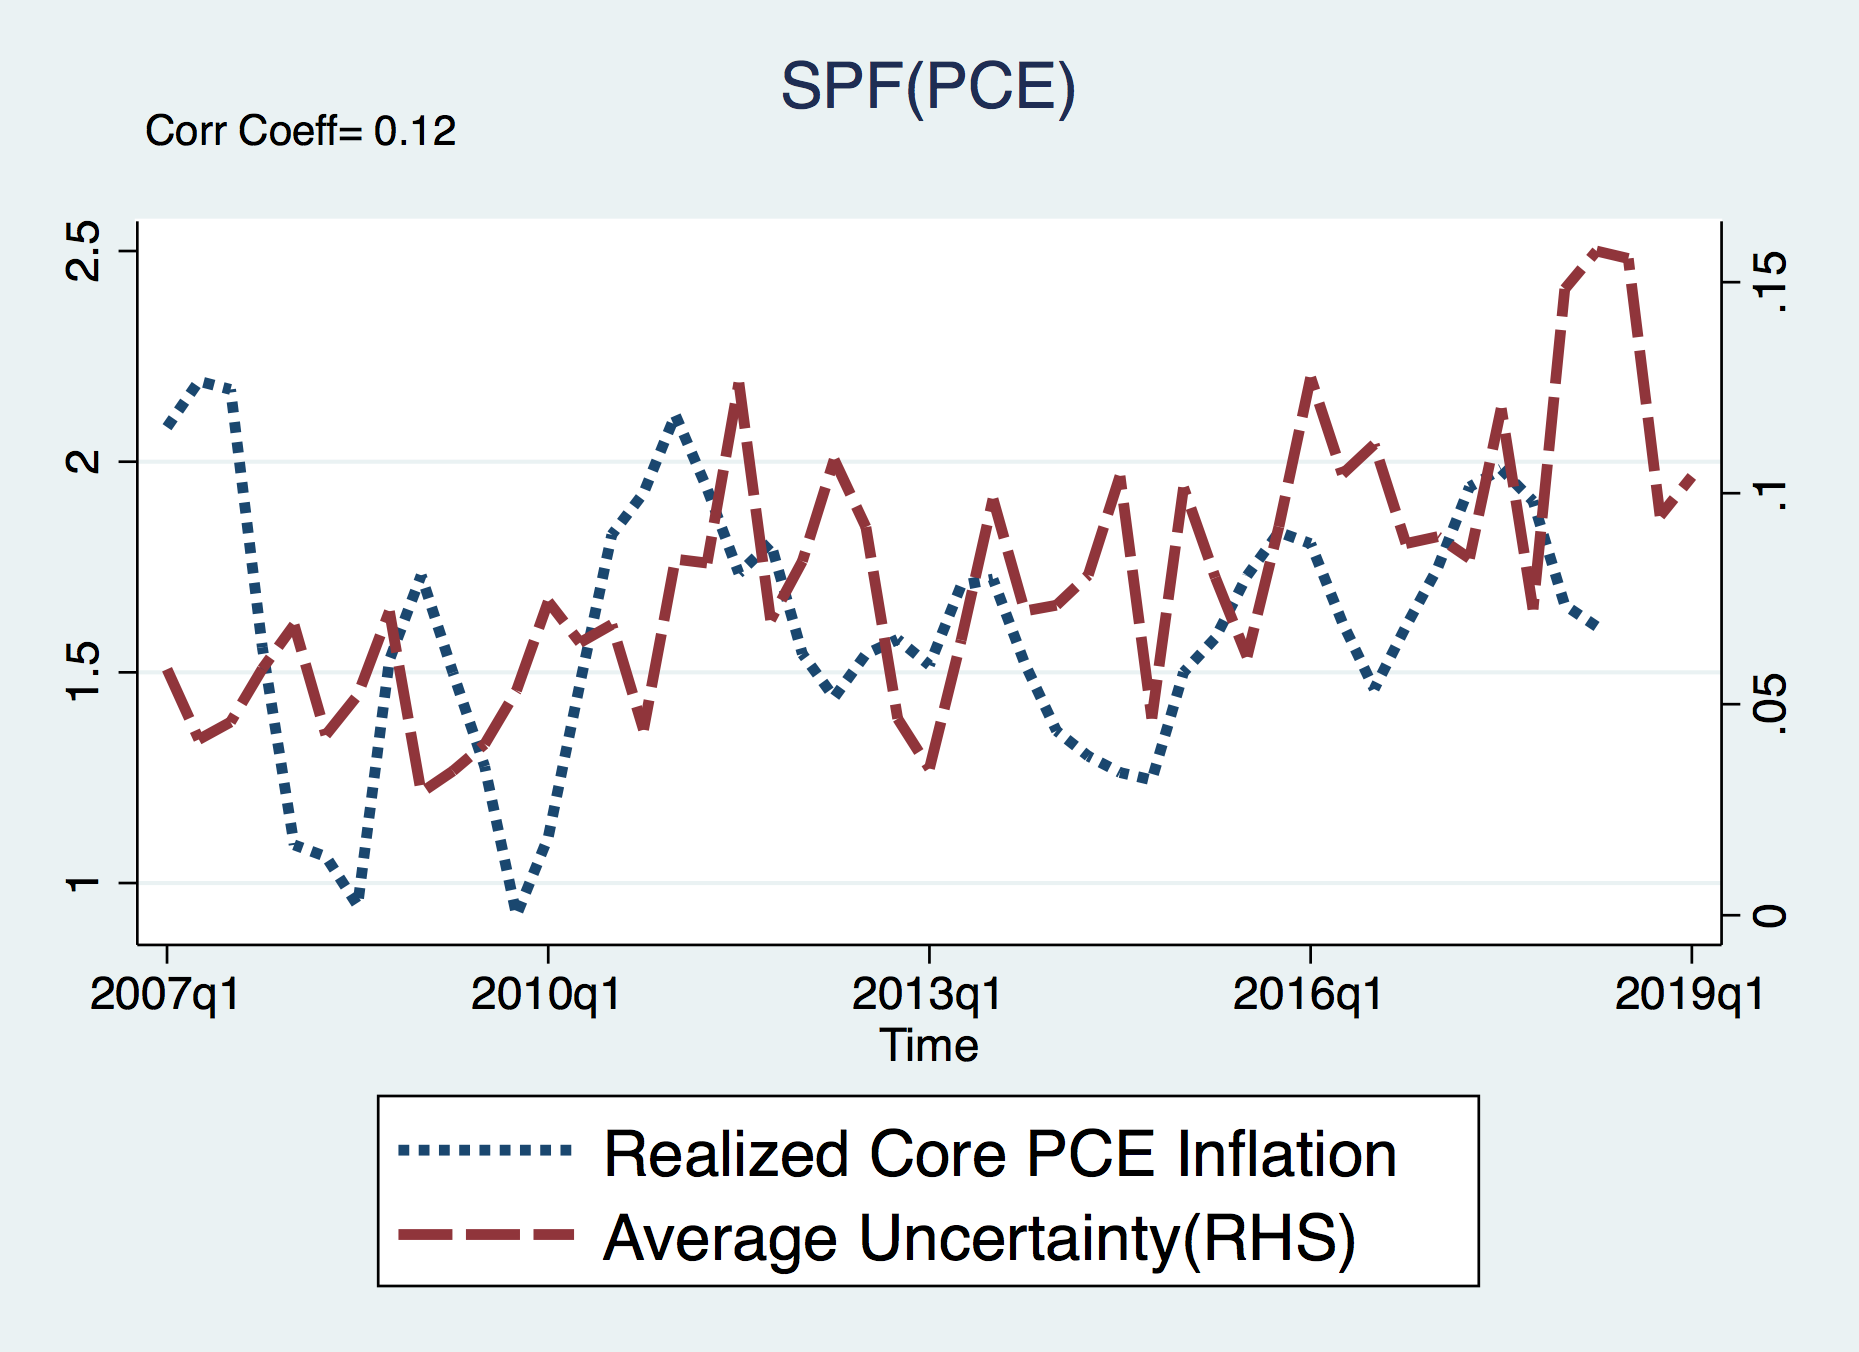
\includegraphics[width=0.3\textwidth]{figures/Inf1yf_PCECore_varSPFPCEQ.png}
			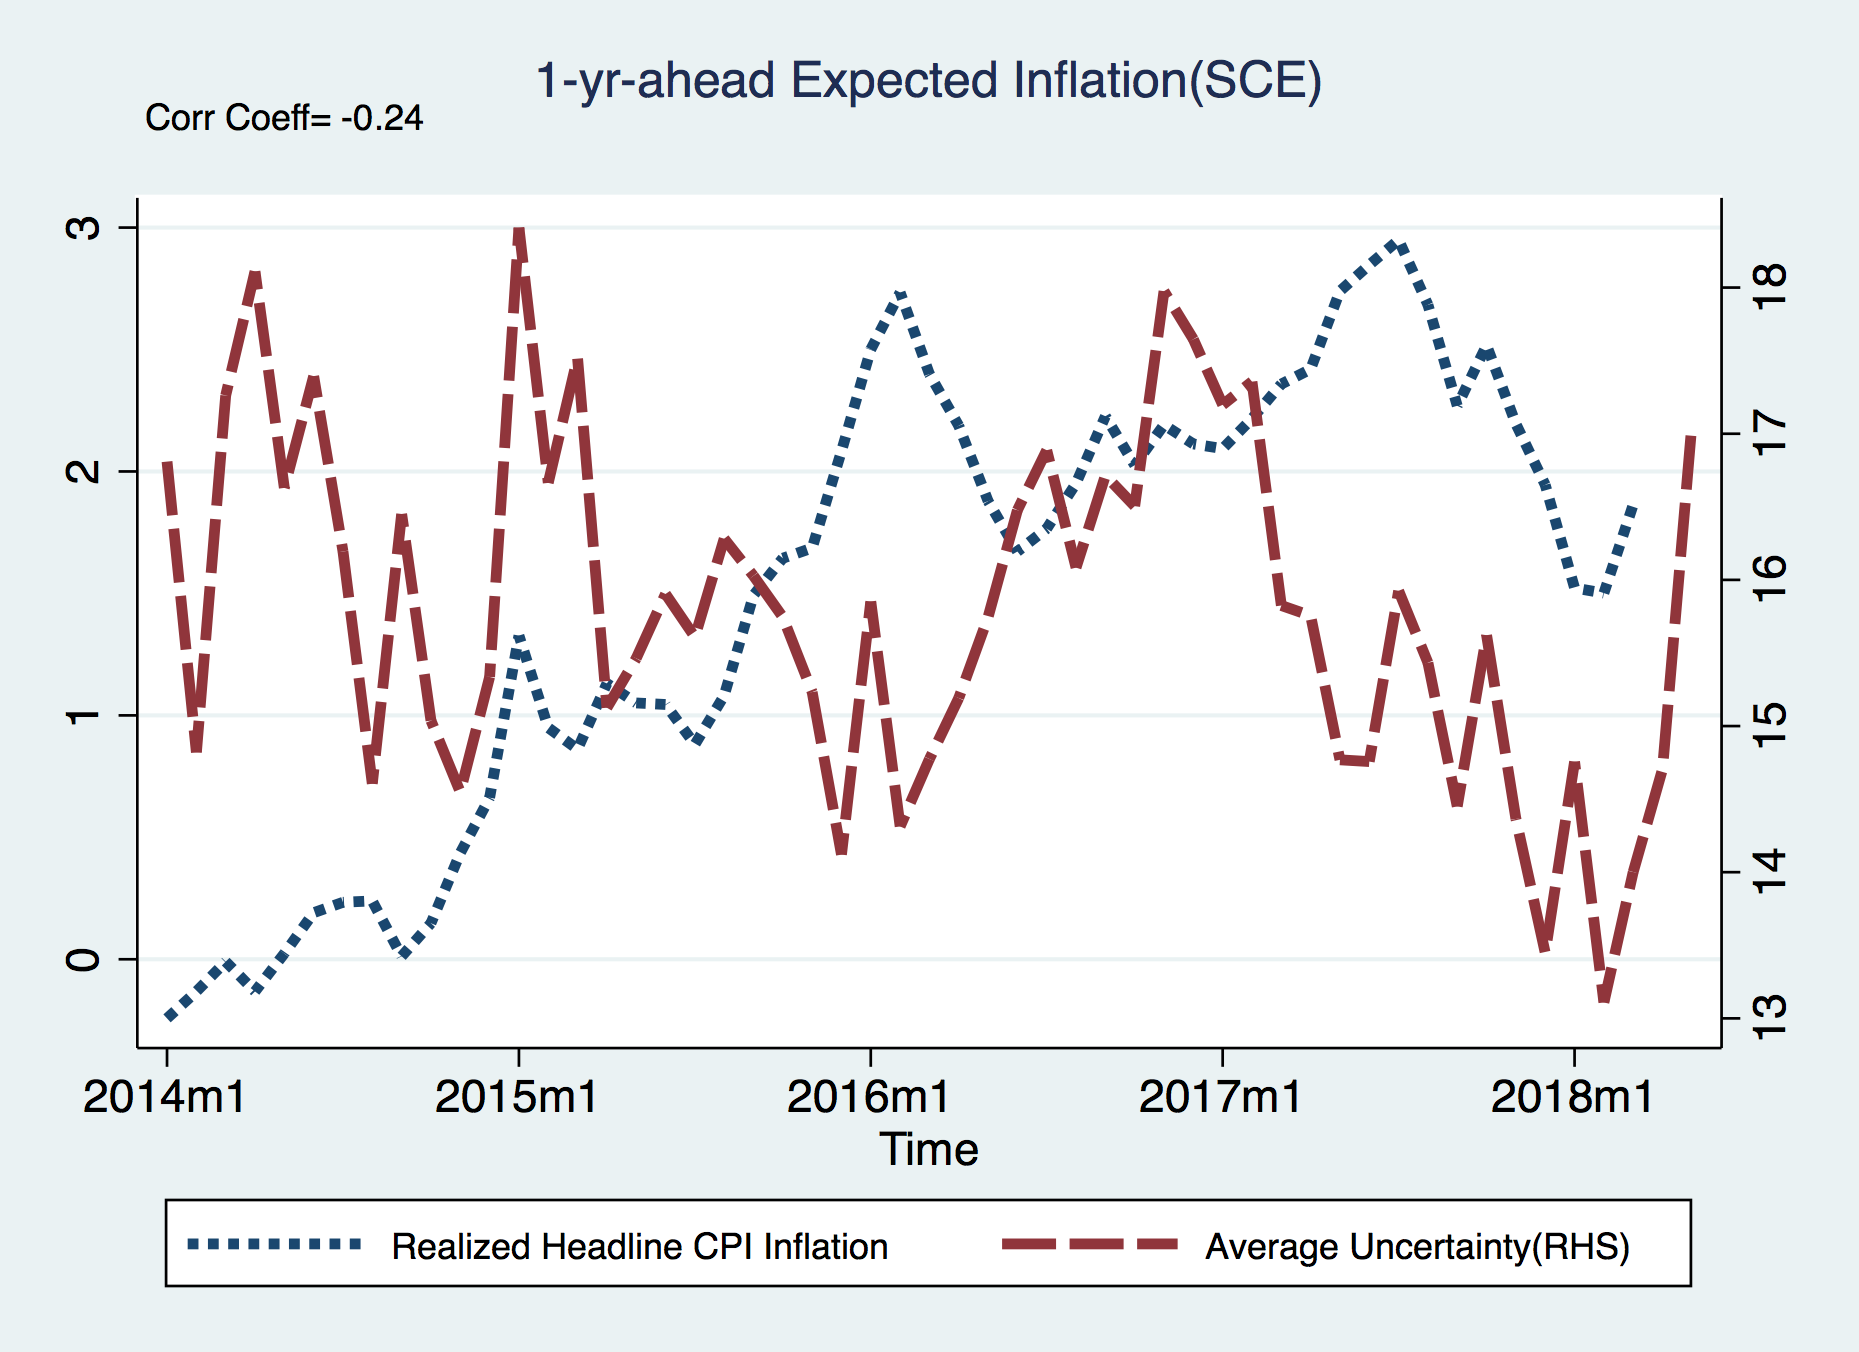
\includegraphics[width=0.3\textwidth]{figures/Inf1yf_CPIAU_varSCEM.png}
		\end{subfigure}
	    \vspace{1em}
		\vfill
		\begin{subfigure}[b]{\textwidth}
			\centering
			\caption{Size of Forecast Errors and Uncertainty}
			\label{FEVar}
			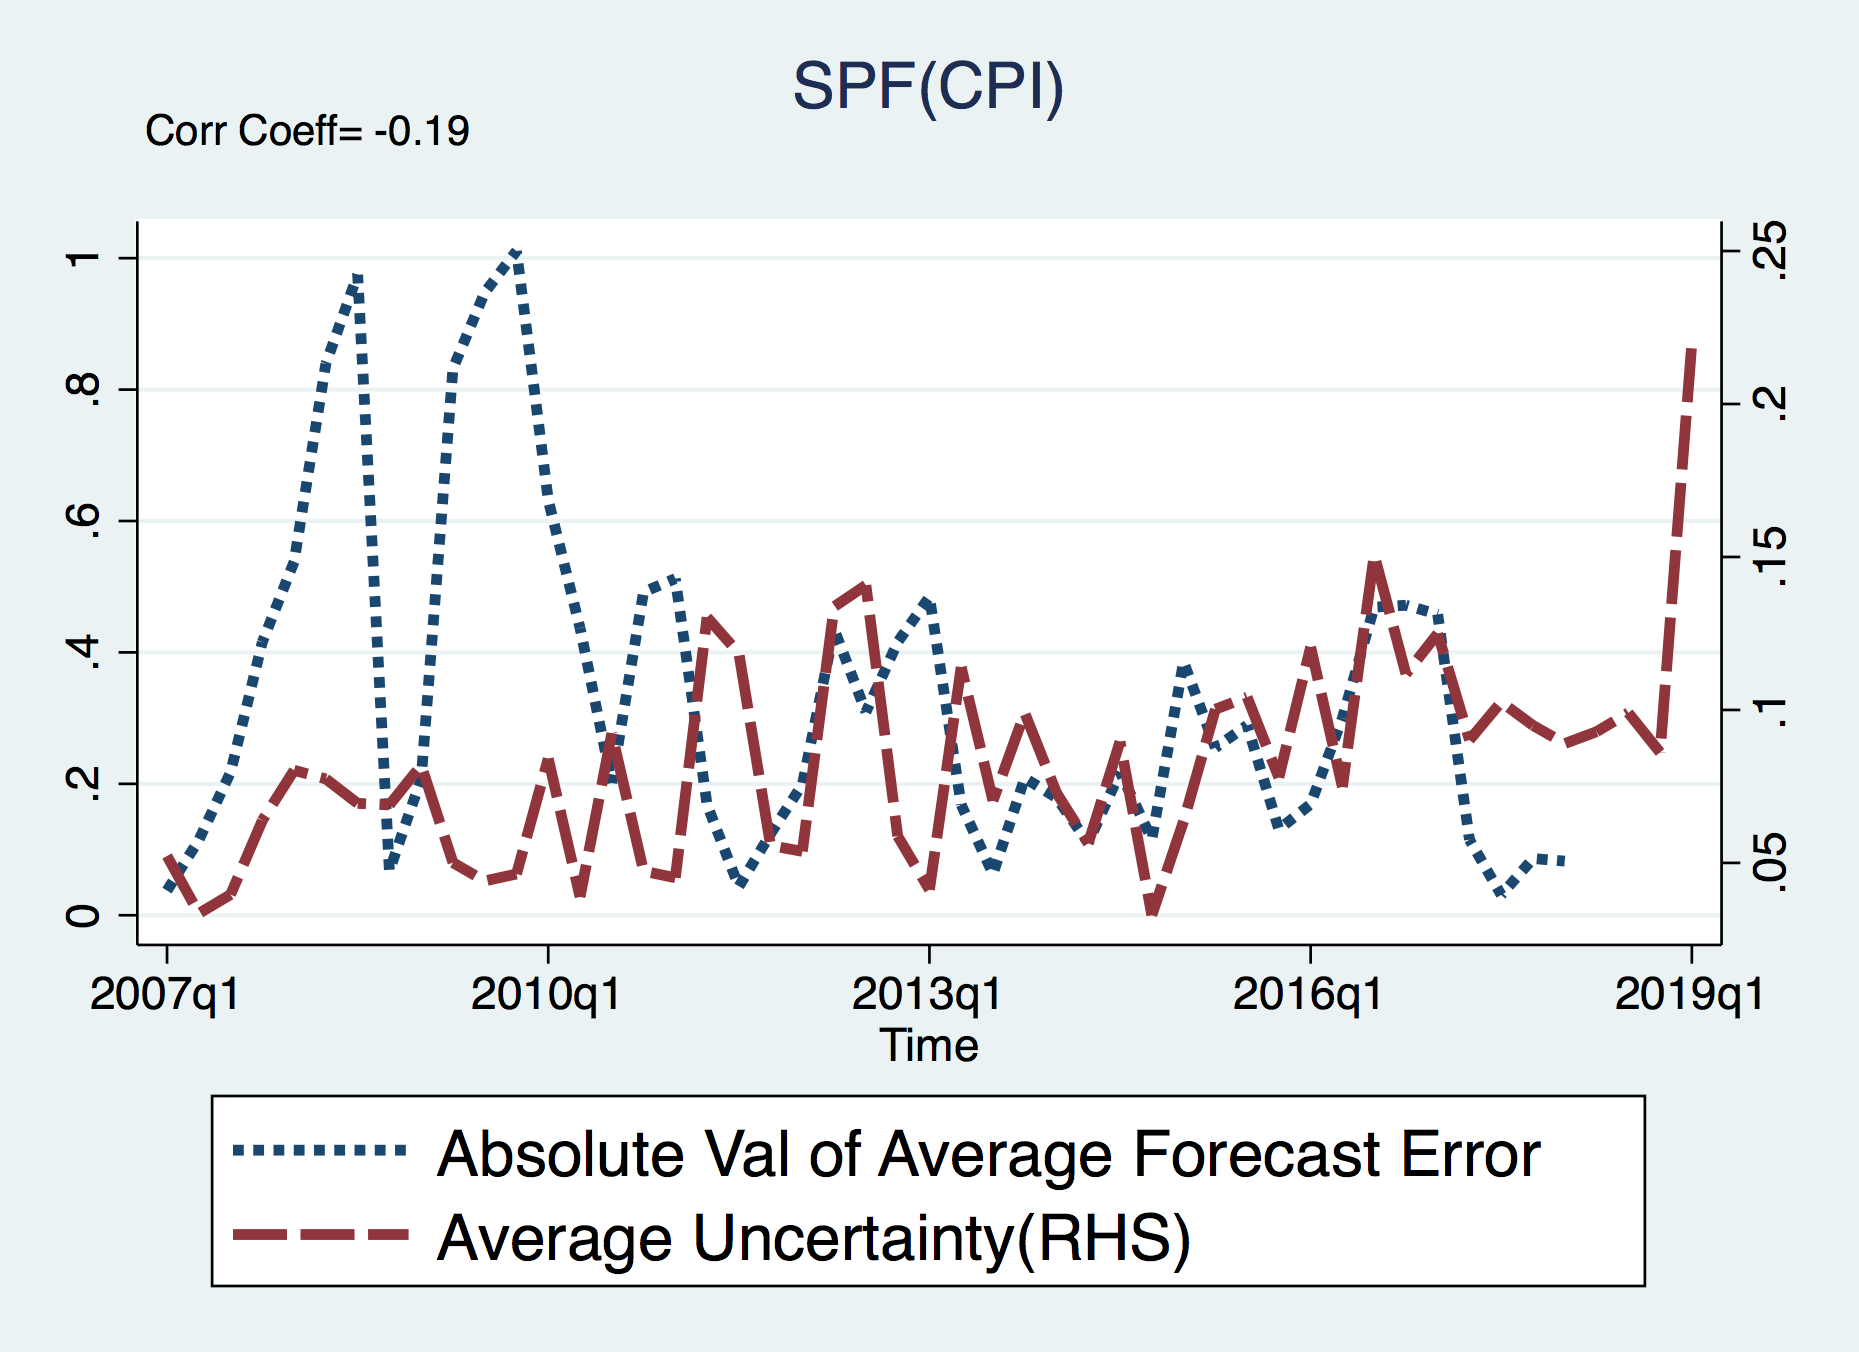
\includegraphics[width=0.3\textwidth]{figures/SPFCPI_abFE_varSPFCPIQ.png}
			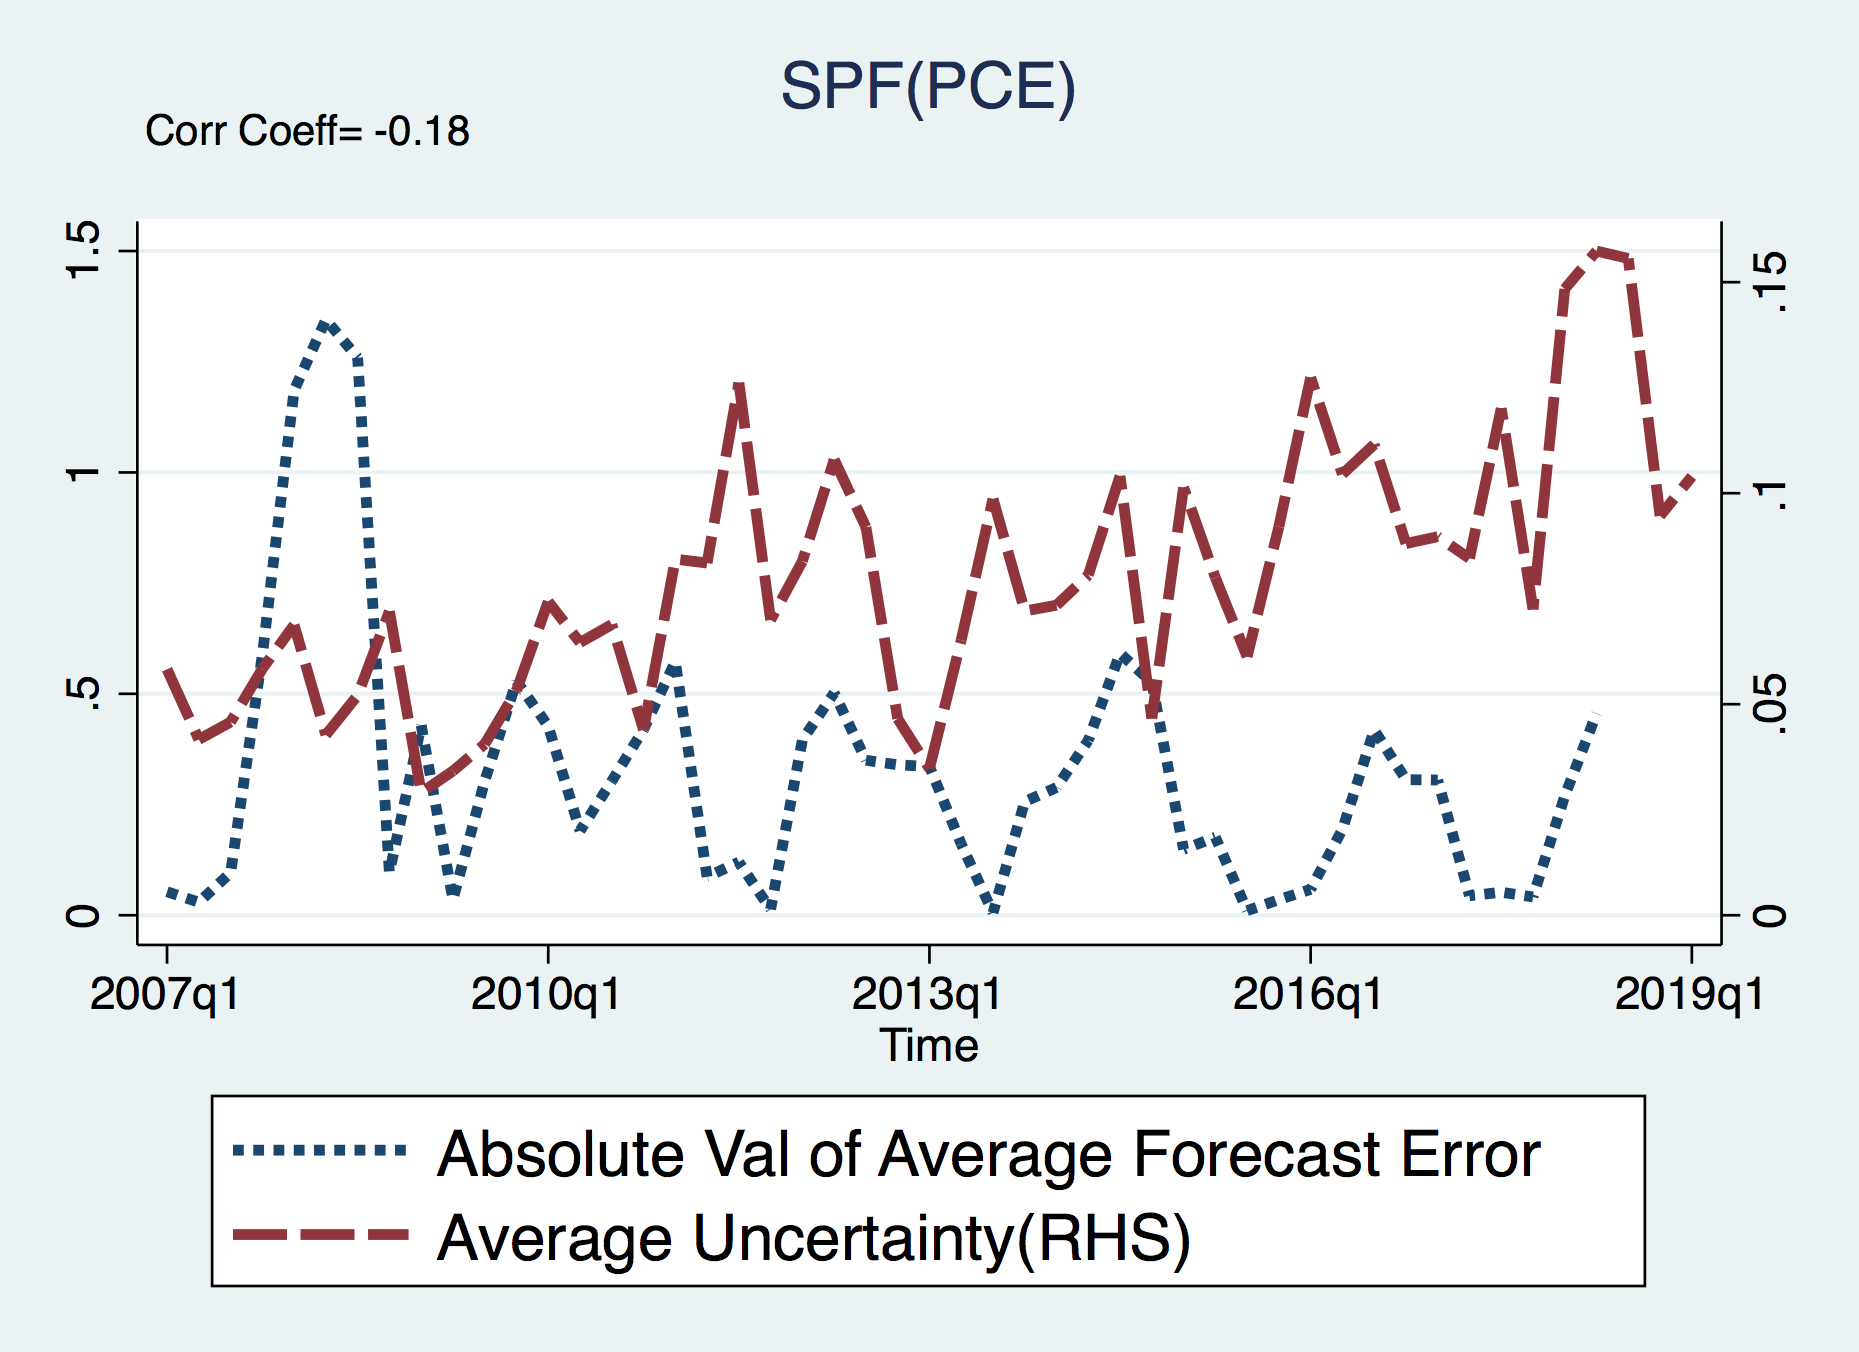
\includegraphics[width=0.3\textwidth]{figures/SPFPCE_abFE_varSPFPCEQ.png}
			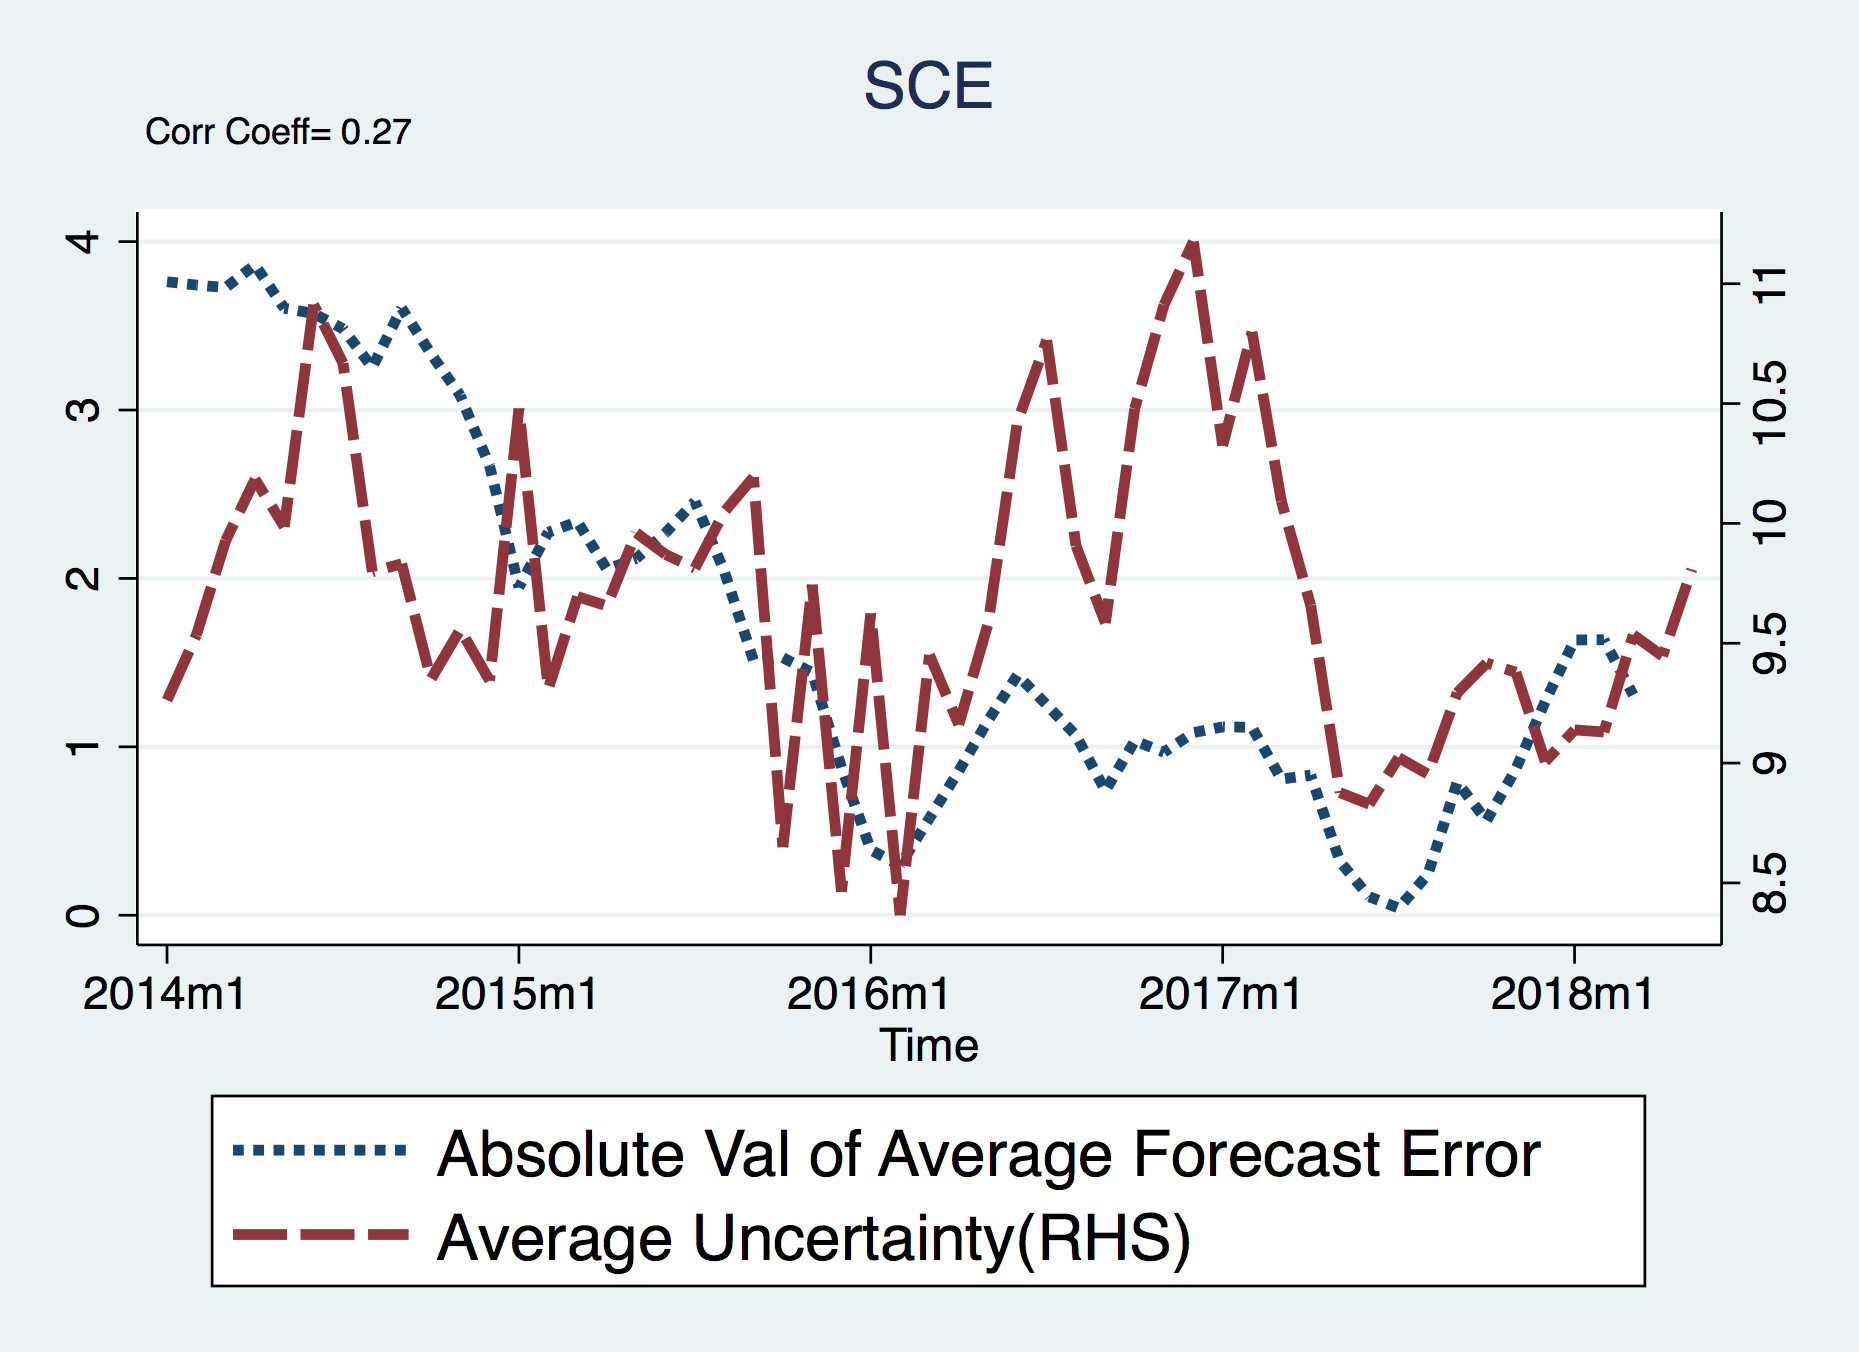
\includegraphics[width=0.3\textwidth]{figures/SCE_abFE_varSCEM.png}
		\end{subfigure}
	 \vspace{0.5em}
		\vfill
		\begin{subfigure}[b]{\textwidth}
			\centering
			\caption{Disagreement and Uncertainty}
			\label{DisgVar}
			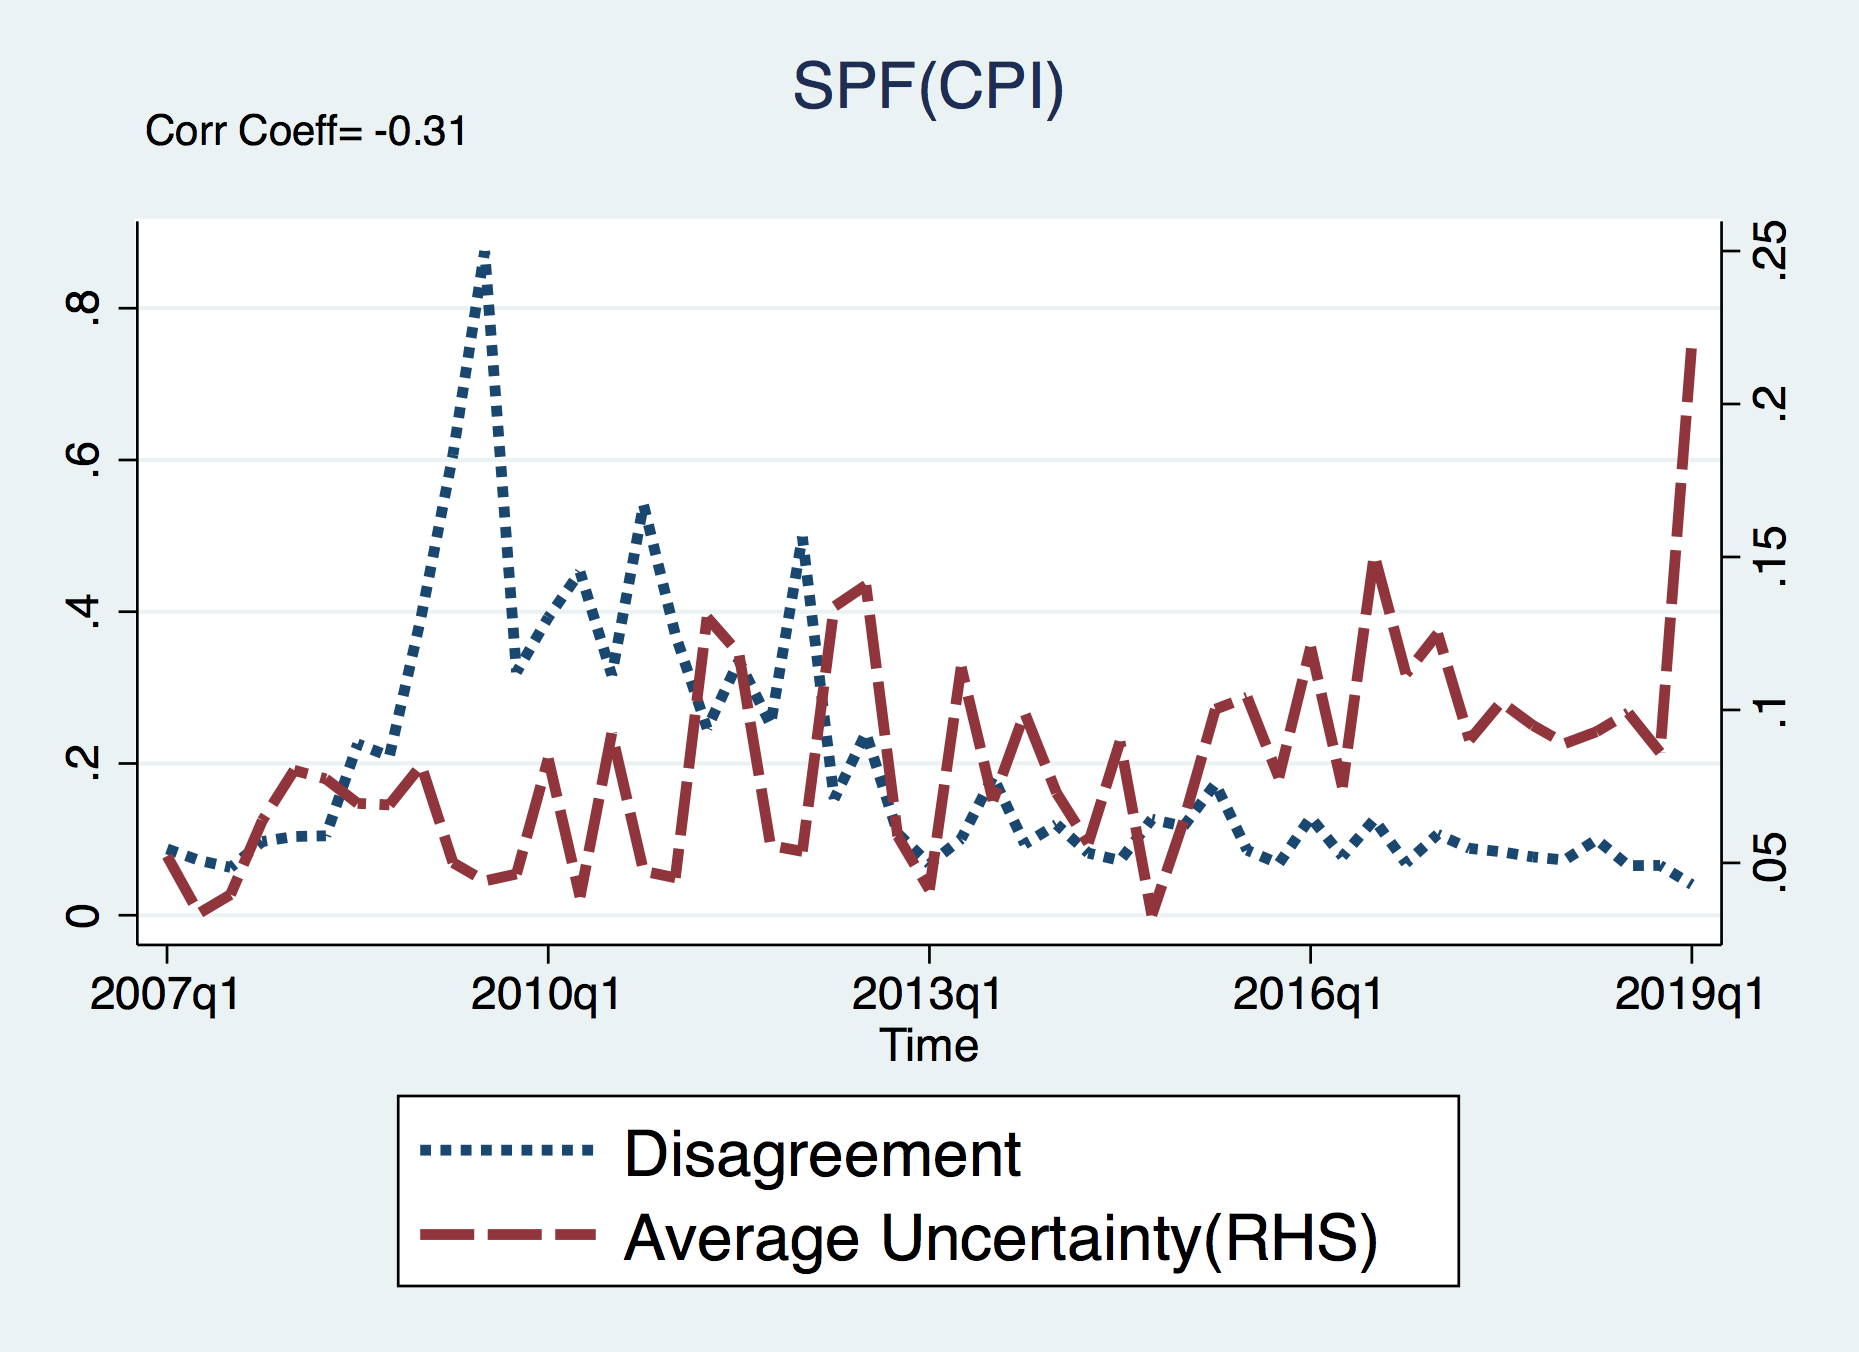
\includegraphics[width=0.3\textwidth]{figures/CORECPI_disg_varSPFCPIQ.png}
			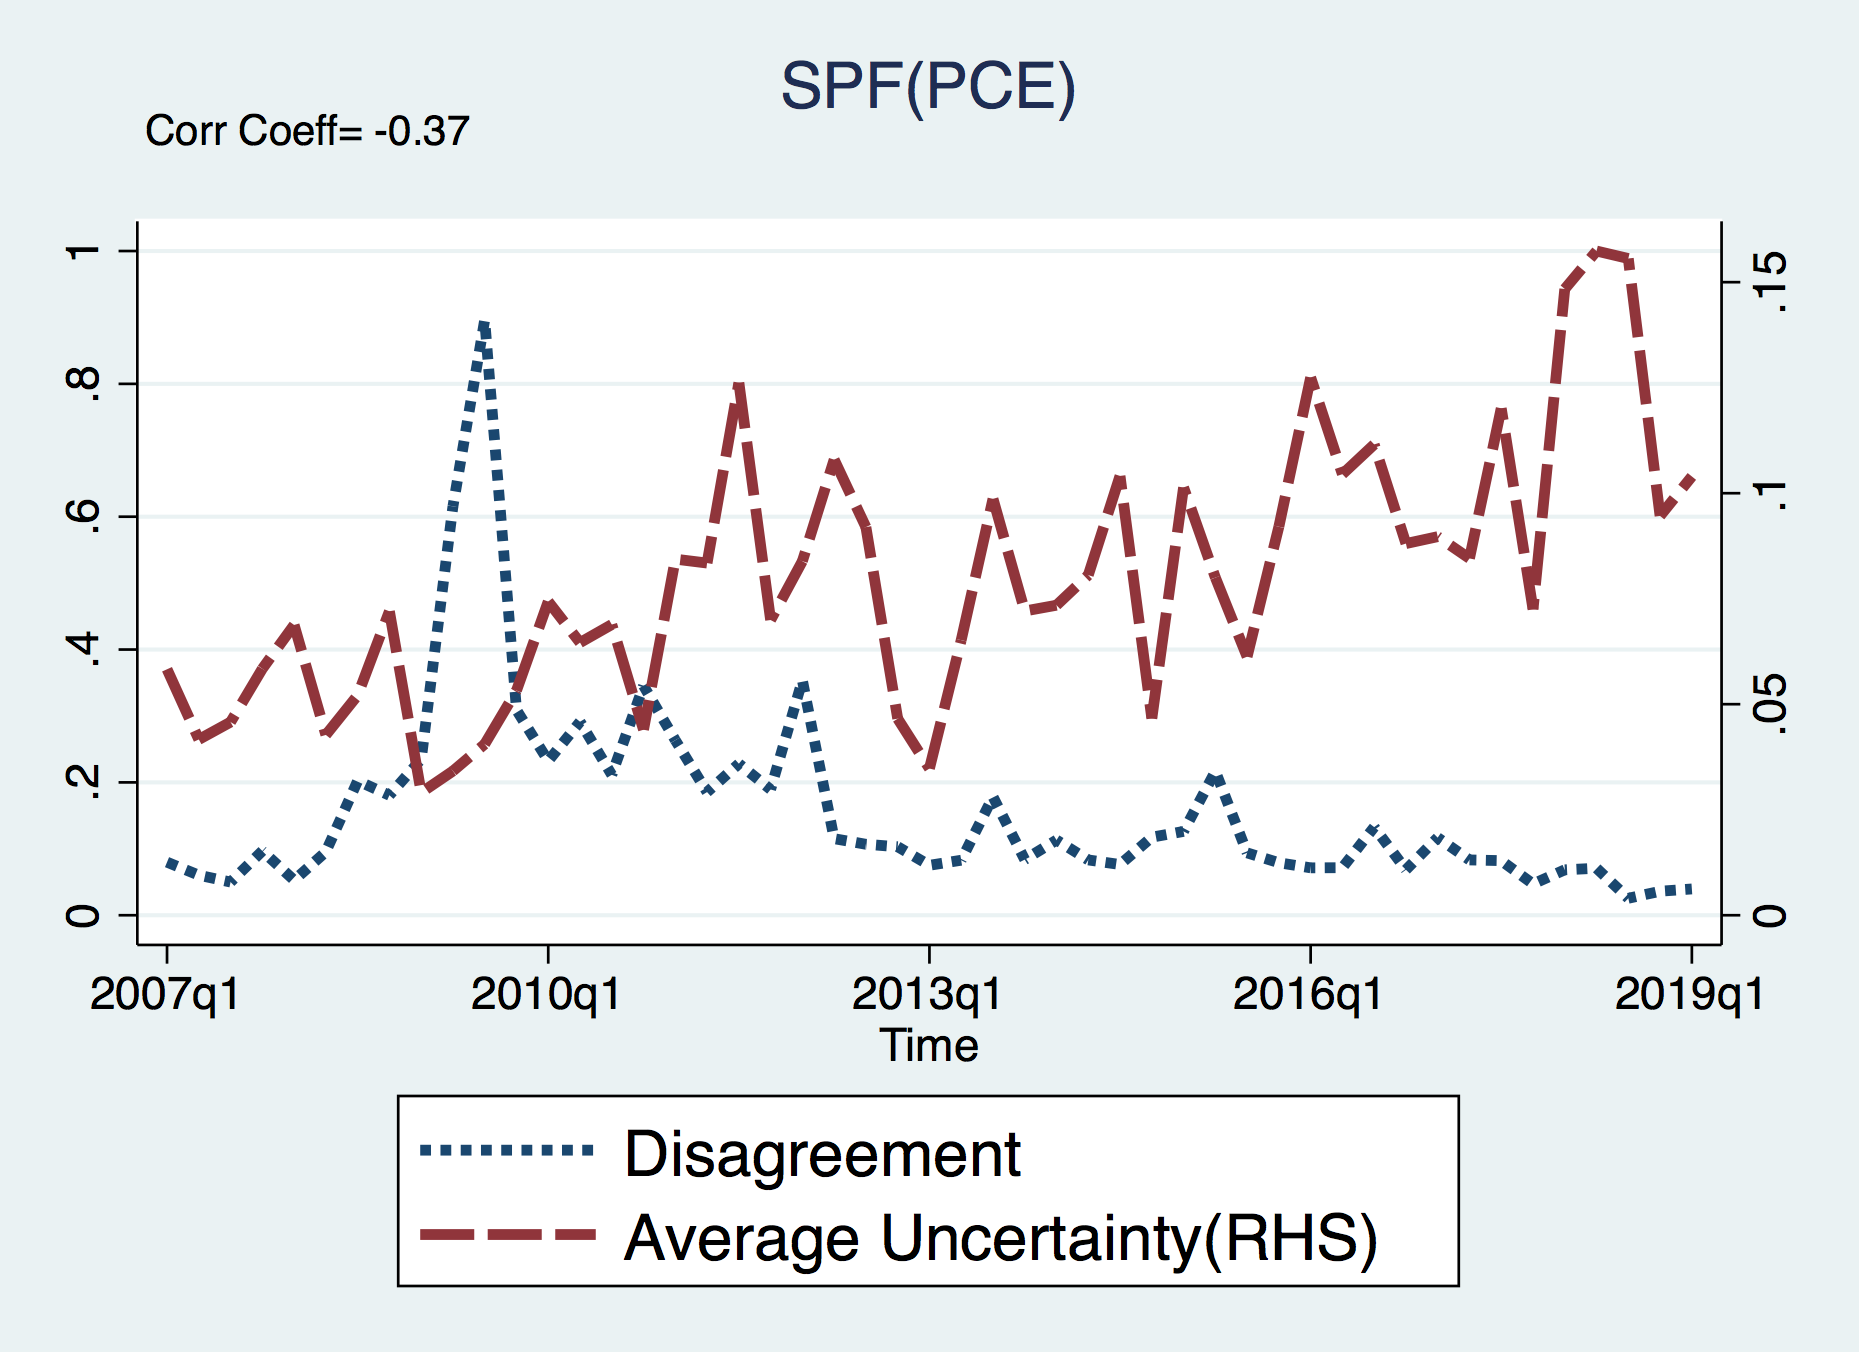
\includegraphics[width=0.3\textwidth]{figures/COREPCE_disg_varSPFPCEQ.png}
			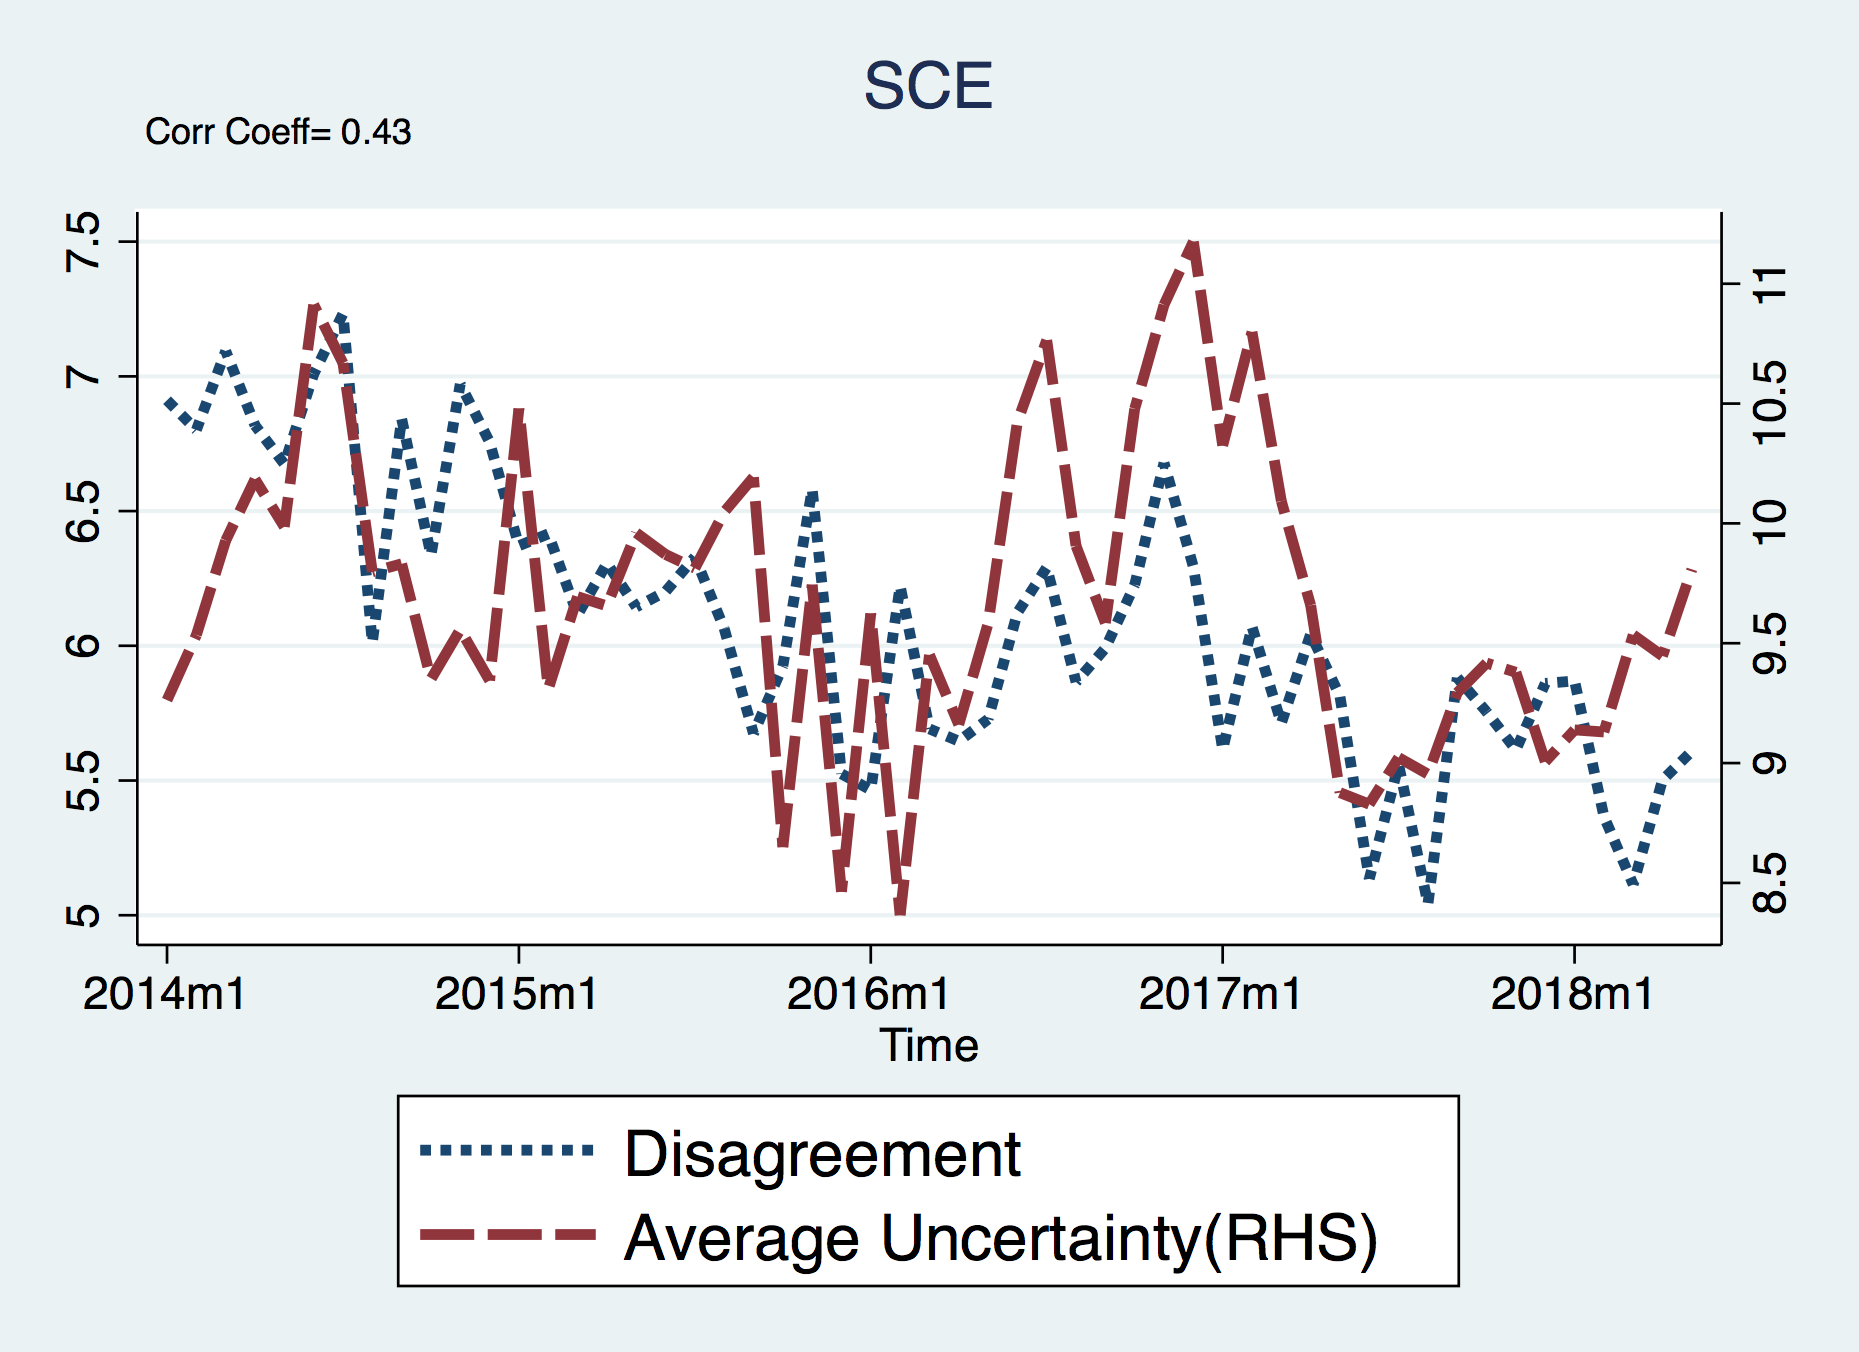
\includegraphics[width=0.3\textwidth]{figures/Q9_disg_varSCEM.png}\\
		\end{subfigure}
		\\
		\begin{flushleft}
			{\footnotesize Note:  From left to right: SPF's  forecasts of core CPI and core PCE, and SCE's forecast of headline CPI. From top to the bottom, uncertainty (red dash) versus realized inflation (blue dot) with correlation coefficient of 0.14, 0.12 and -0.25, respectively; uncertainty (red dash) versus absolute value of forecast errors (blue dot) with correlation coefficient of -0.19, -0.18, 0.27, respectively; uncertainty (red dash) versus  disagreements (blue dot) with correlation coefficient of -0.31, -0.37 and 0.43,repectively. Only the Pearson tests of correlation between disagreement and uncertainty are significant for all.}
		\end{flushleft}
		\caption{Uncertainty and Other Moments}
		\label{UnceratitnyOtherMoments}
	\end{figure}
	
	
	\begin{figure}[ht]
		\begin{subfigure}[b]{0.5\textwidth}
		\centering
		\caption{Mean Forecasts}
		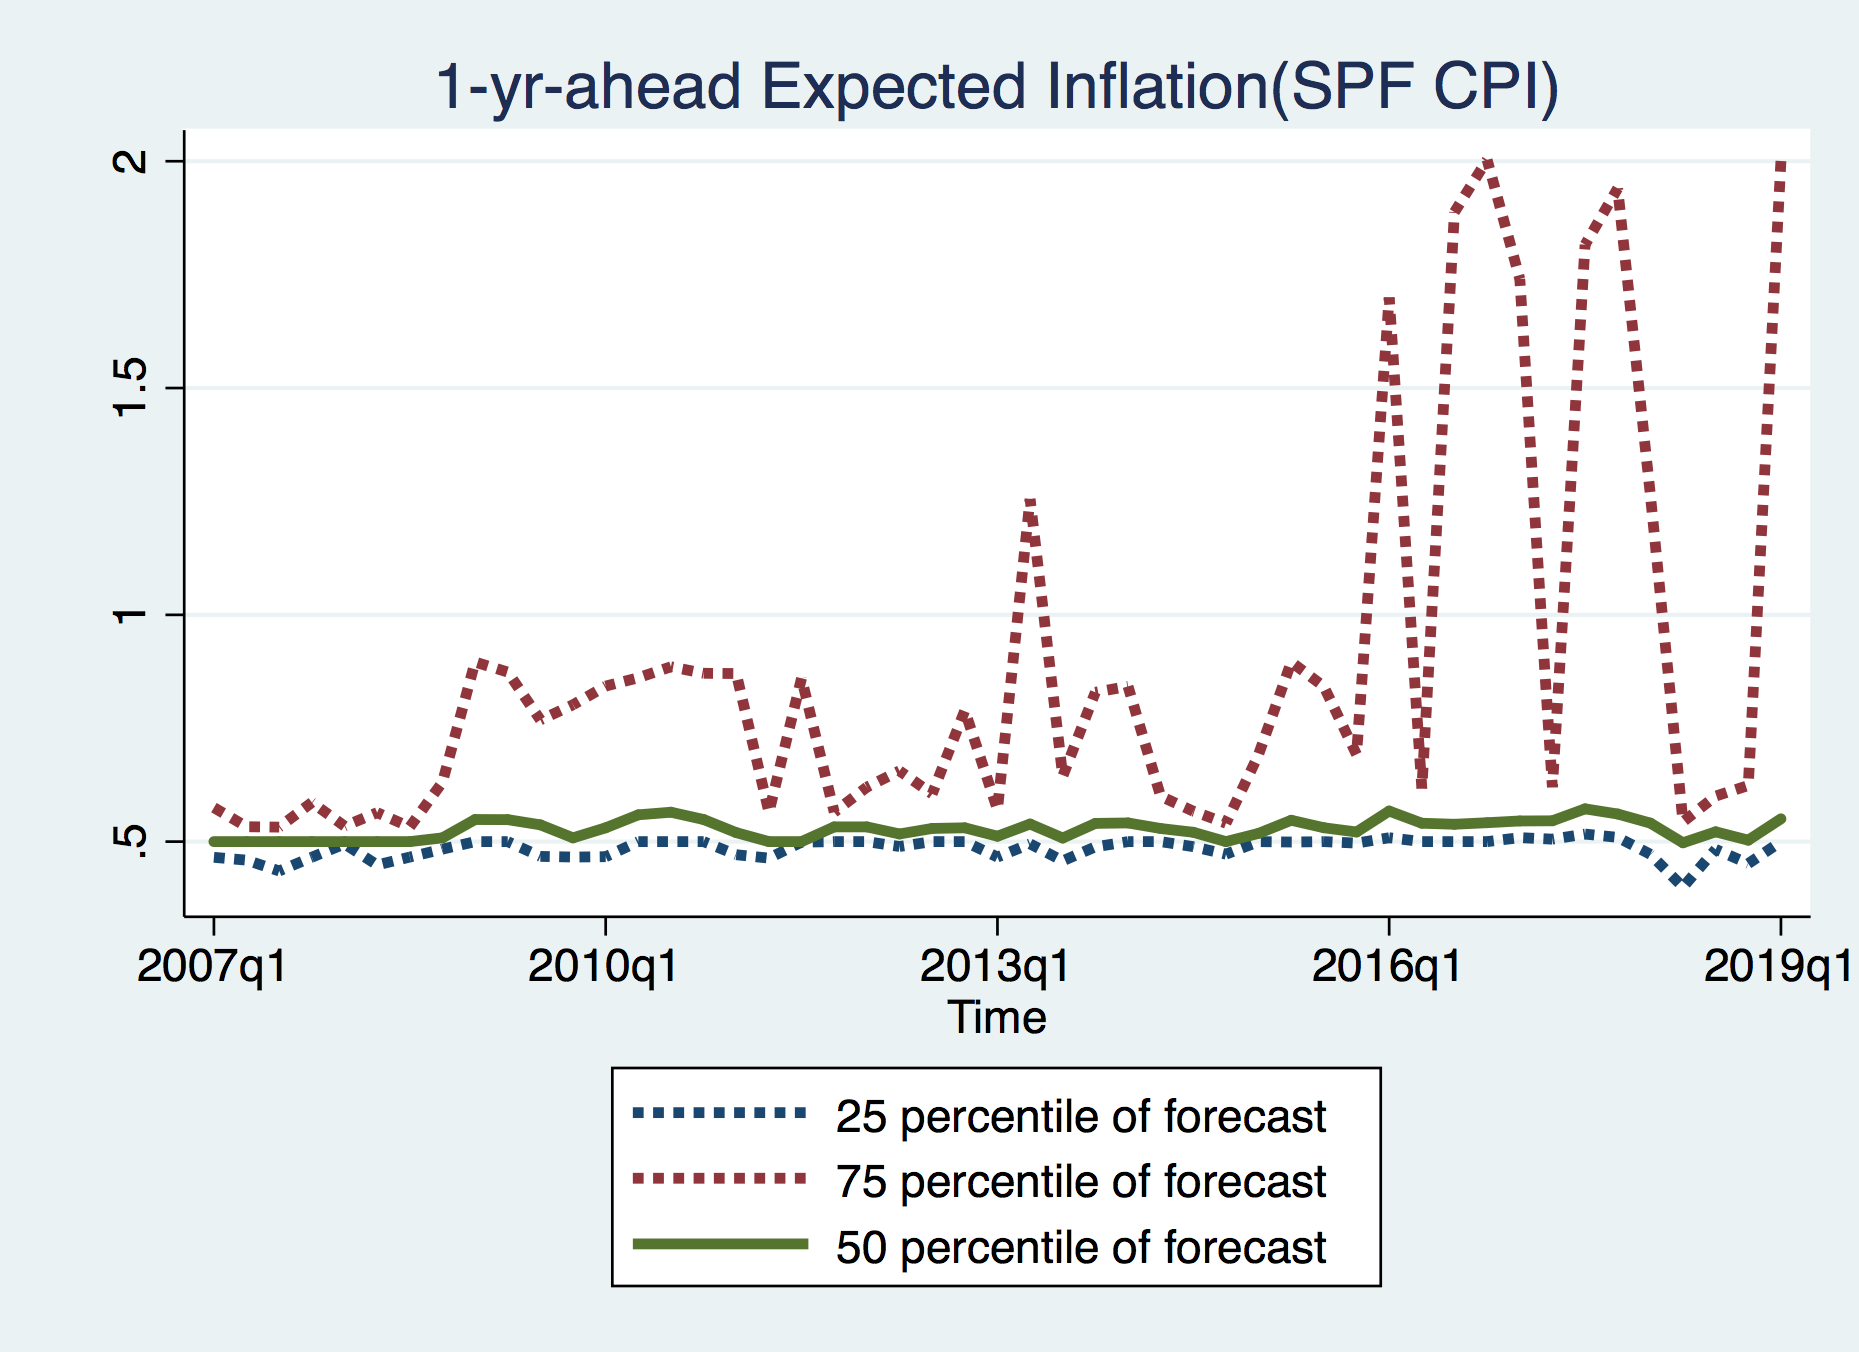
\includegraphics[width=7cm]{figures/IQRmeanCPIQ.png} 
		\smallskip
		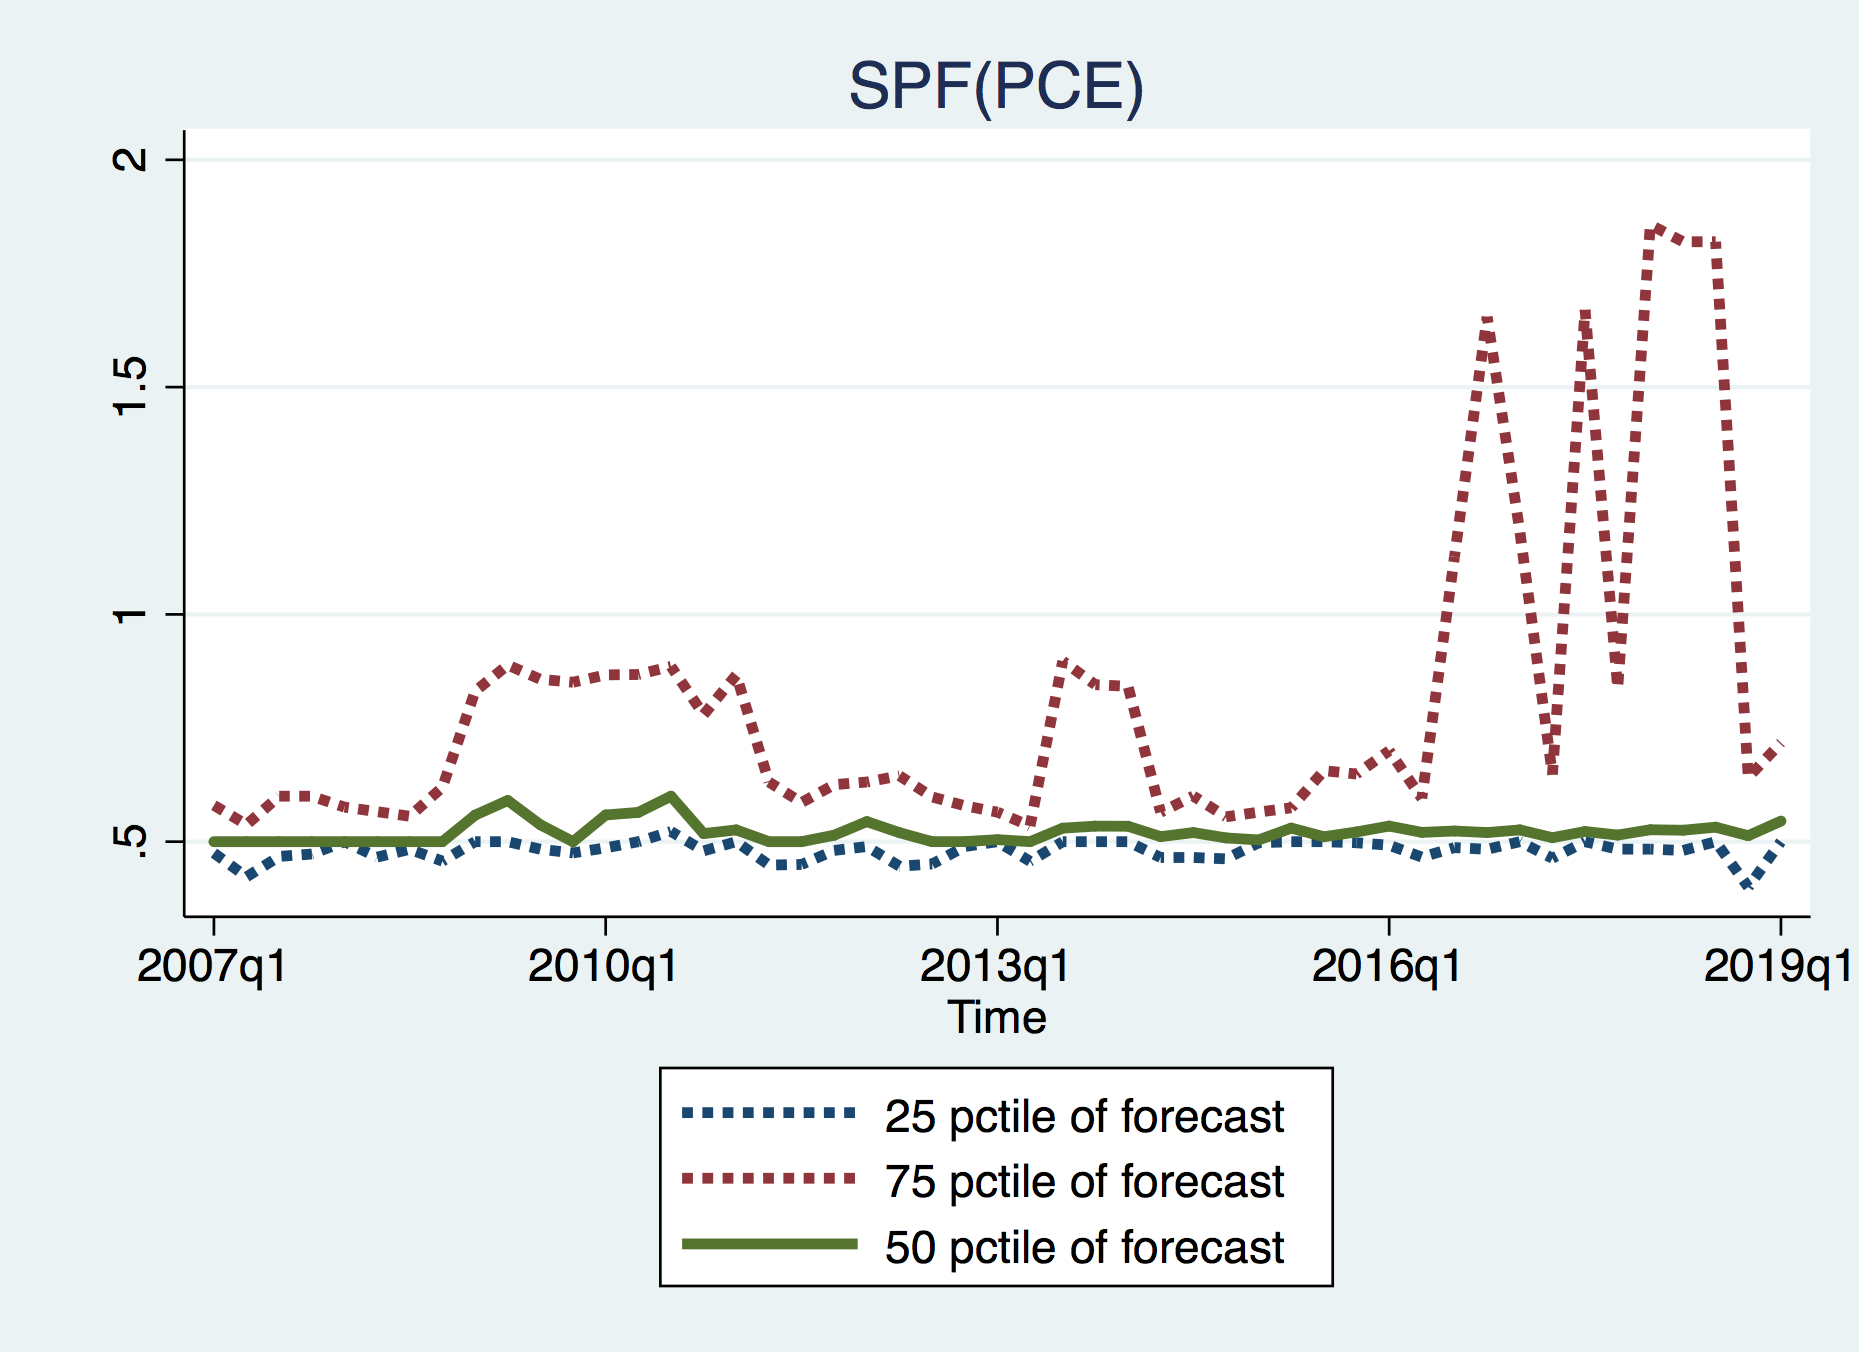
\includegraphics[width=7cm]{figures/IQRmeanPCEQ.png}
		\smallskip
		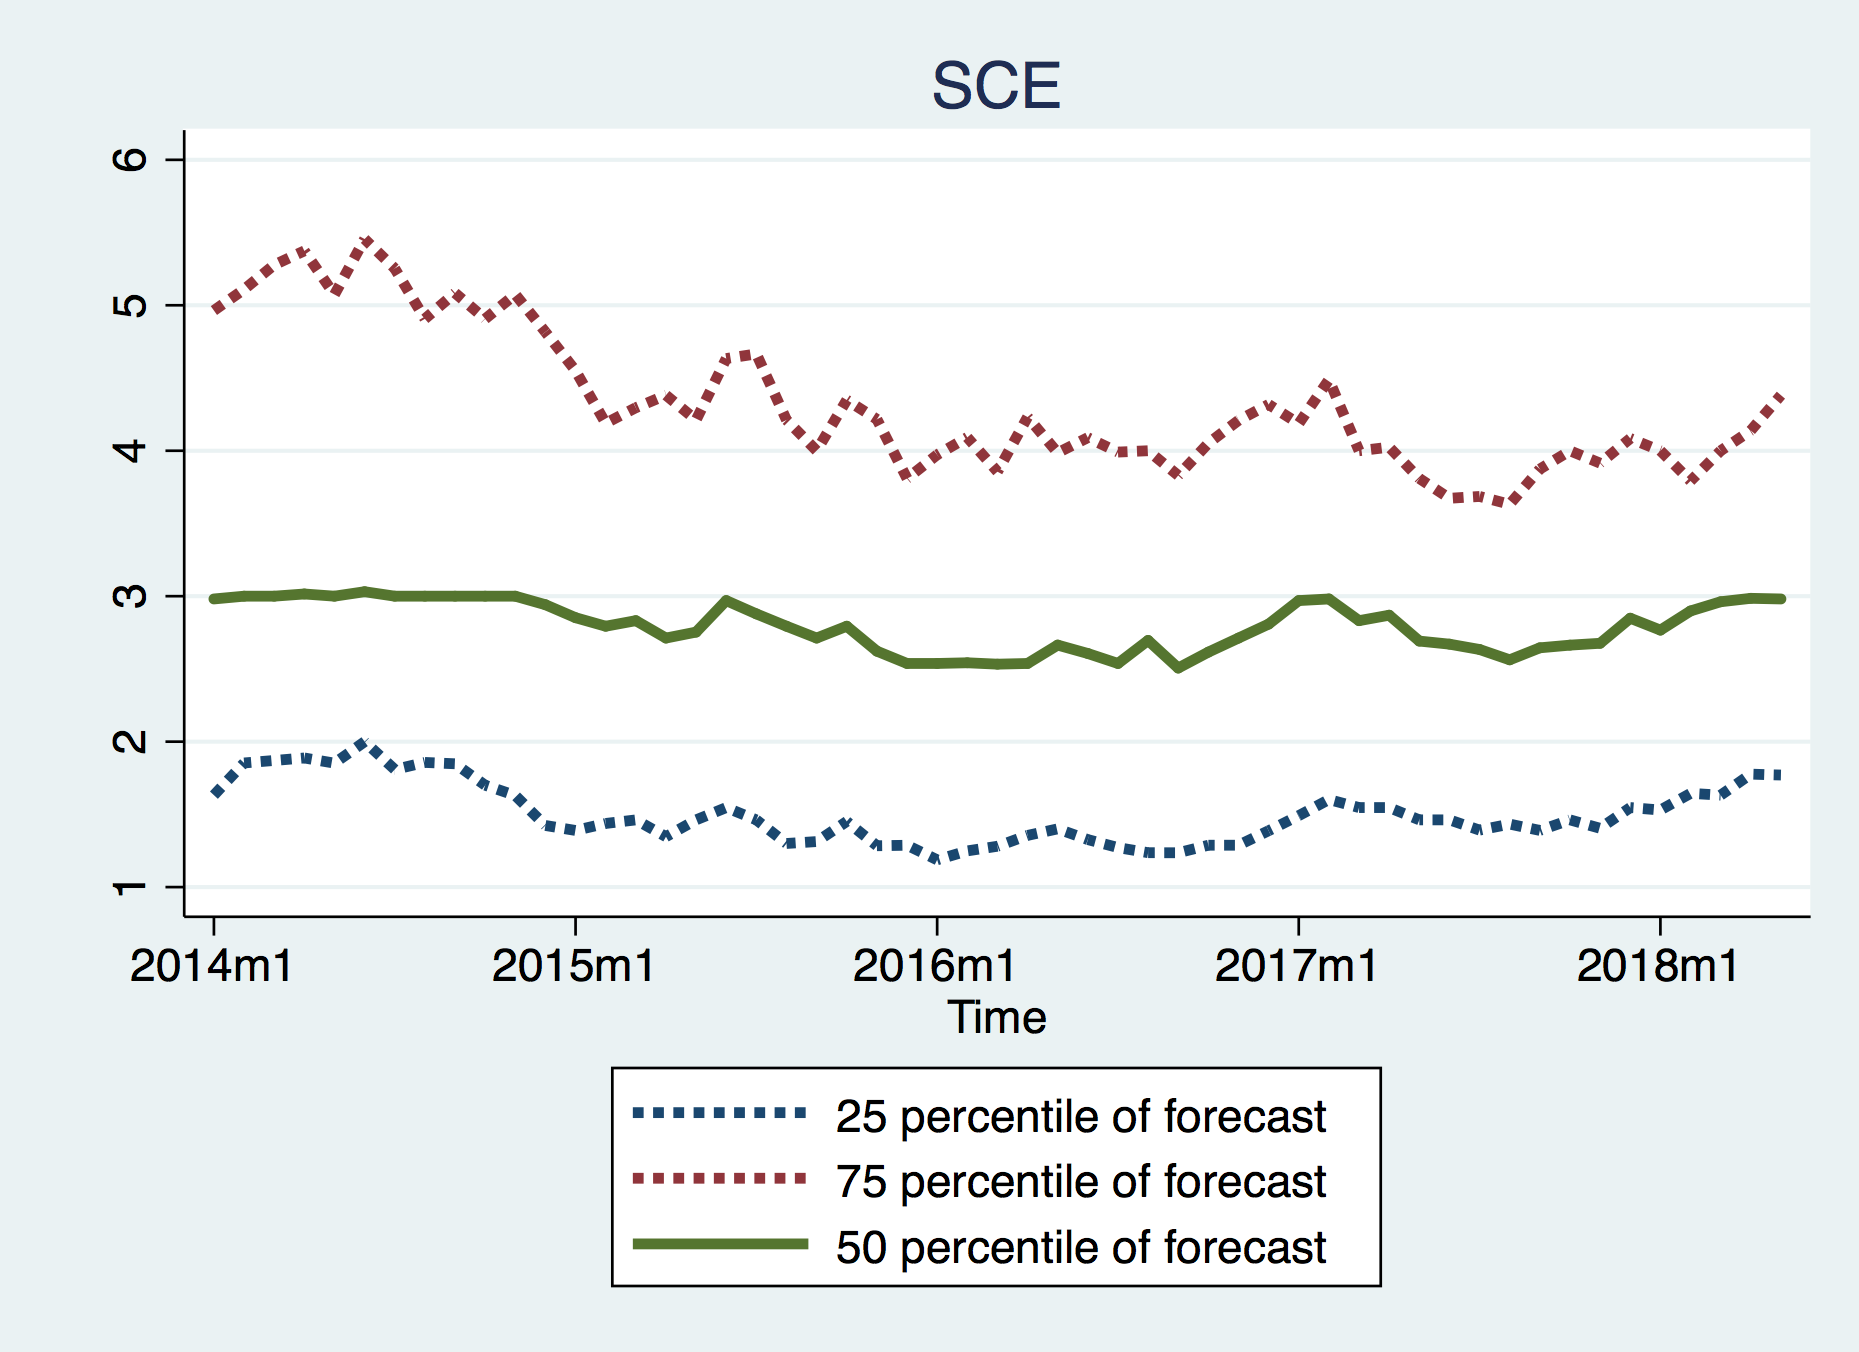
\includegraphics[width=7cm]{figures/IQRmeanSCEM.png}
		\end{subfigure}
	    \hfill 
		\begin{subfigure}[b]{0.5\textwidth}
		\centering 
		\caption{Uncertainty}
		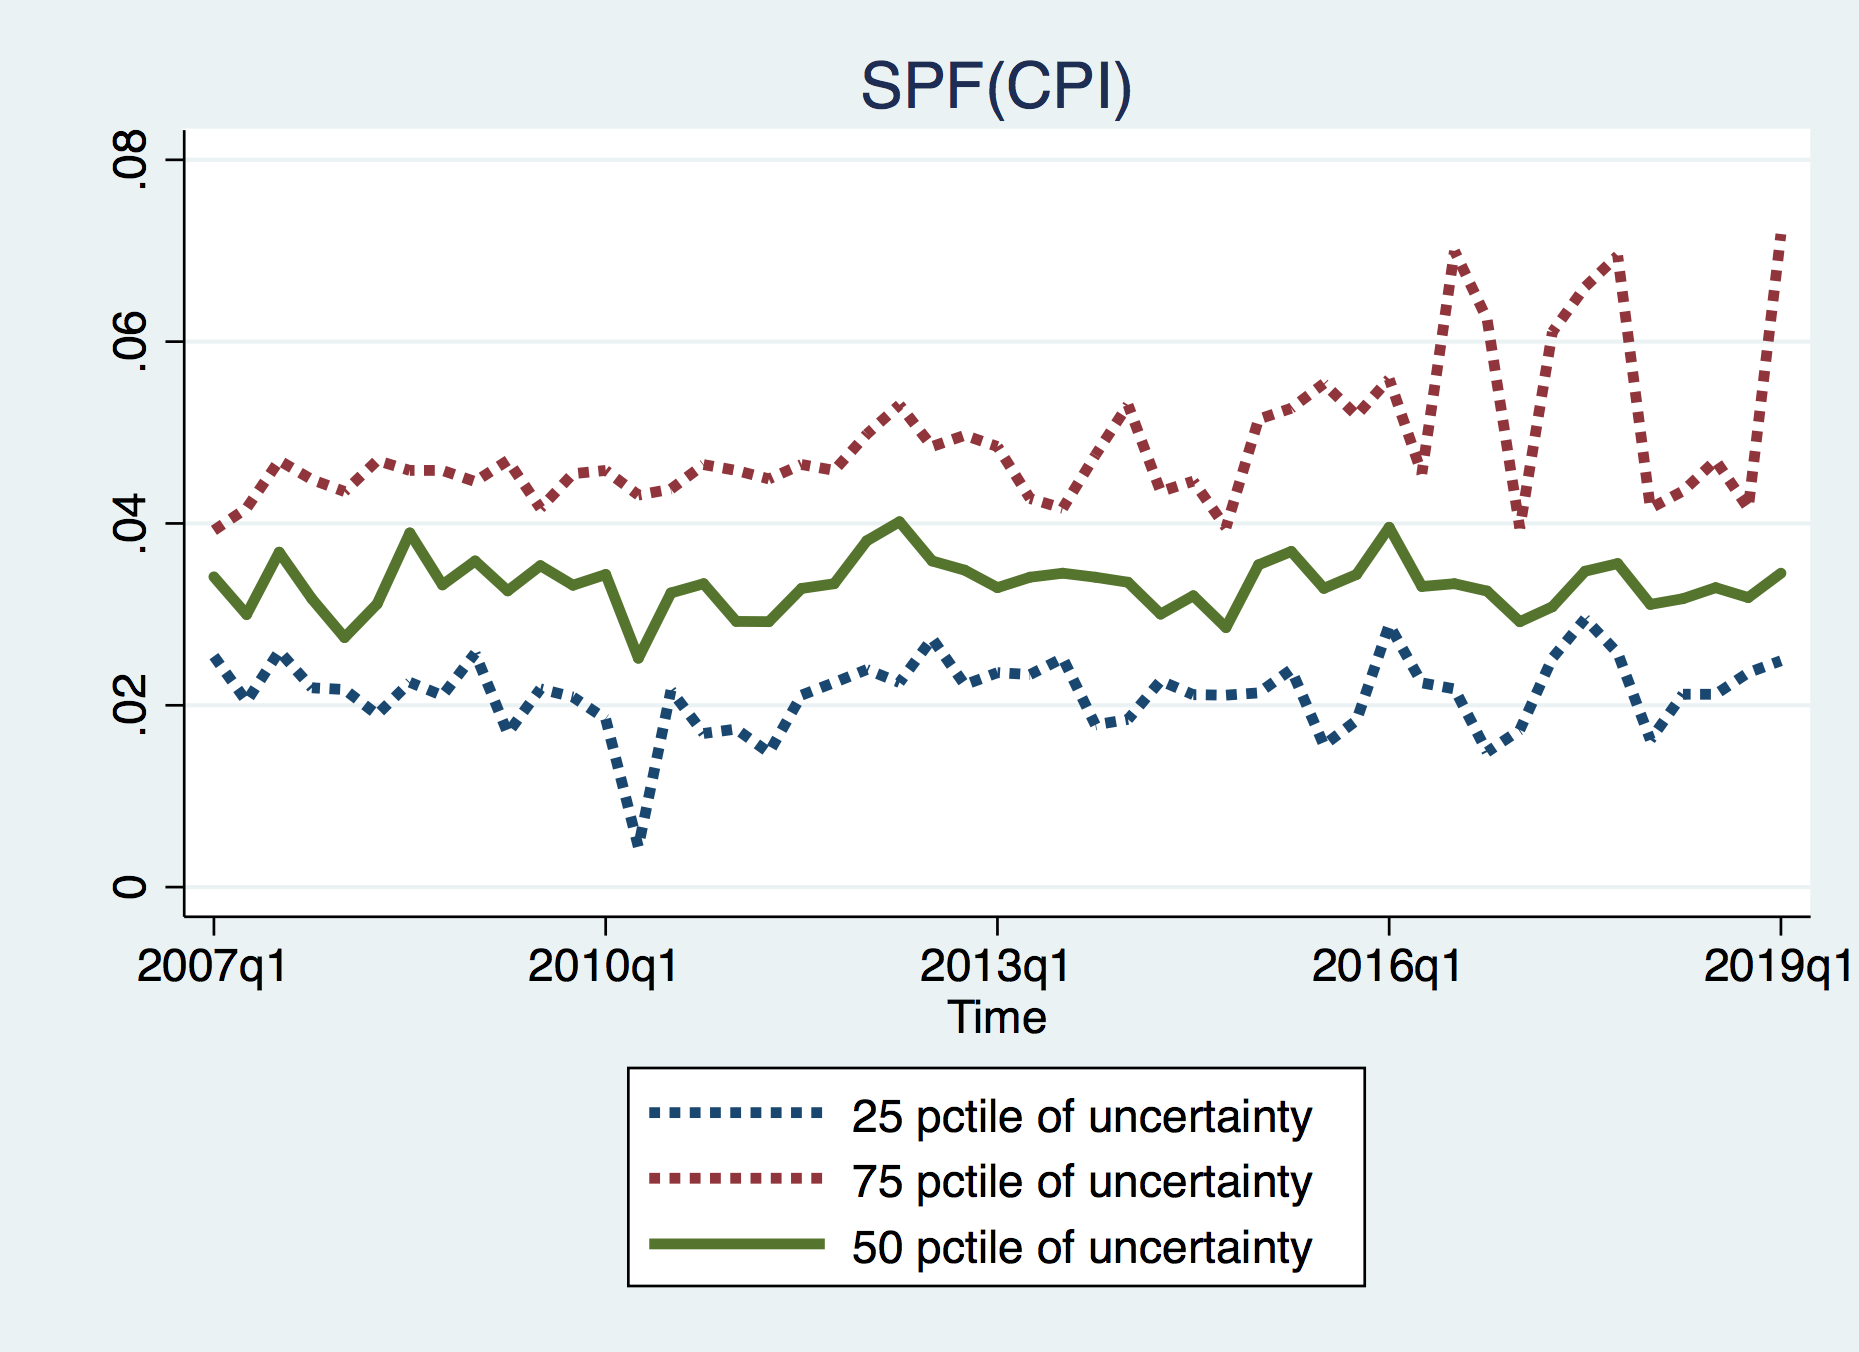
\includegraphics[width=7cm]{figures/IQRvarCPIQ.png}
		\smallskip
		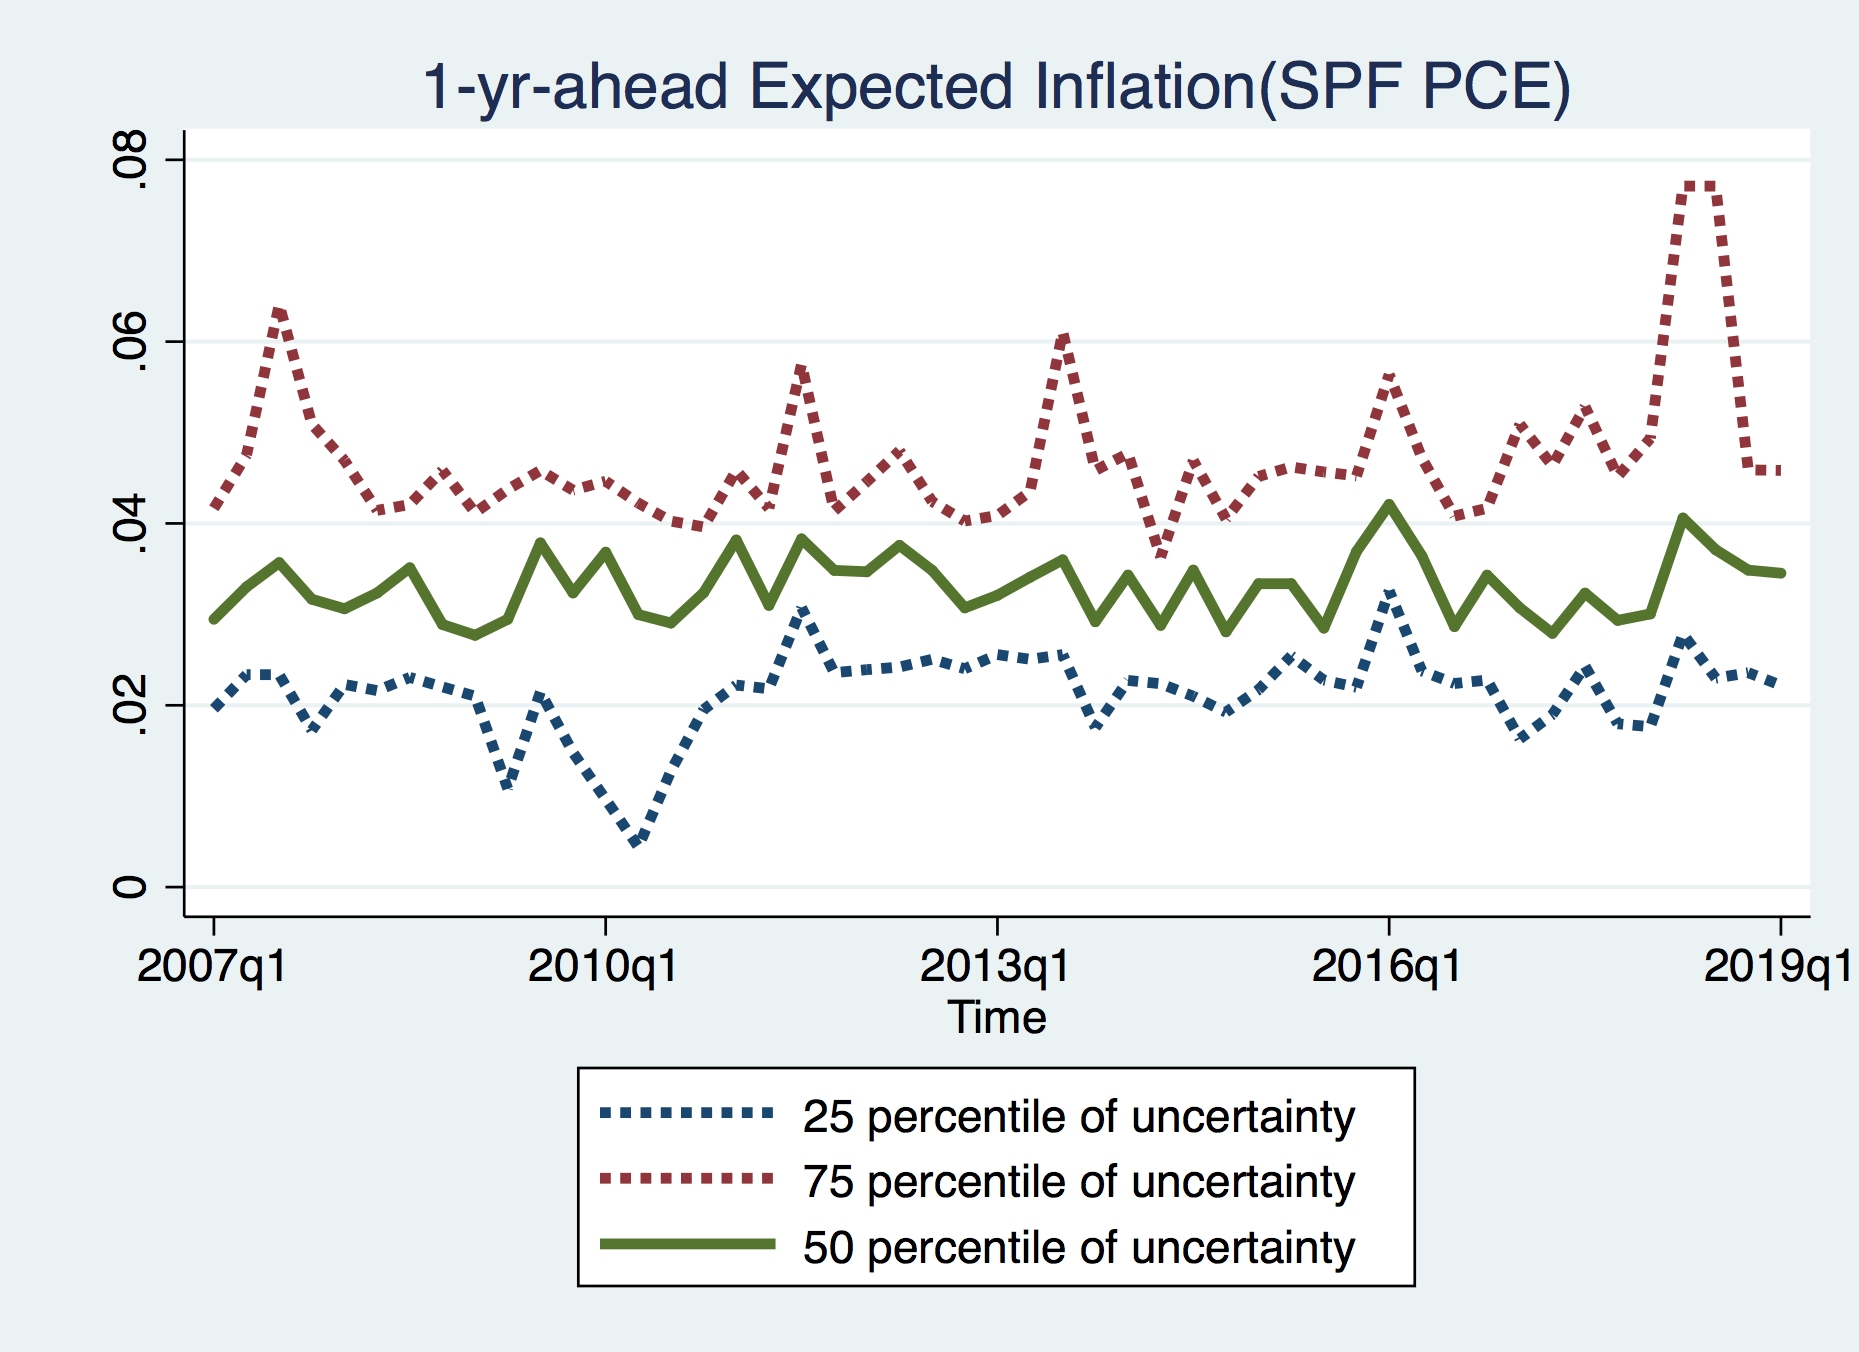
\includegraphics[width=7cm]{figures/IQRvarPCEQ.png}
		\smallskip
		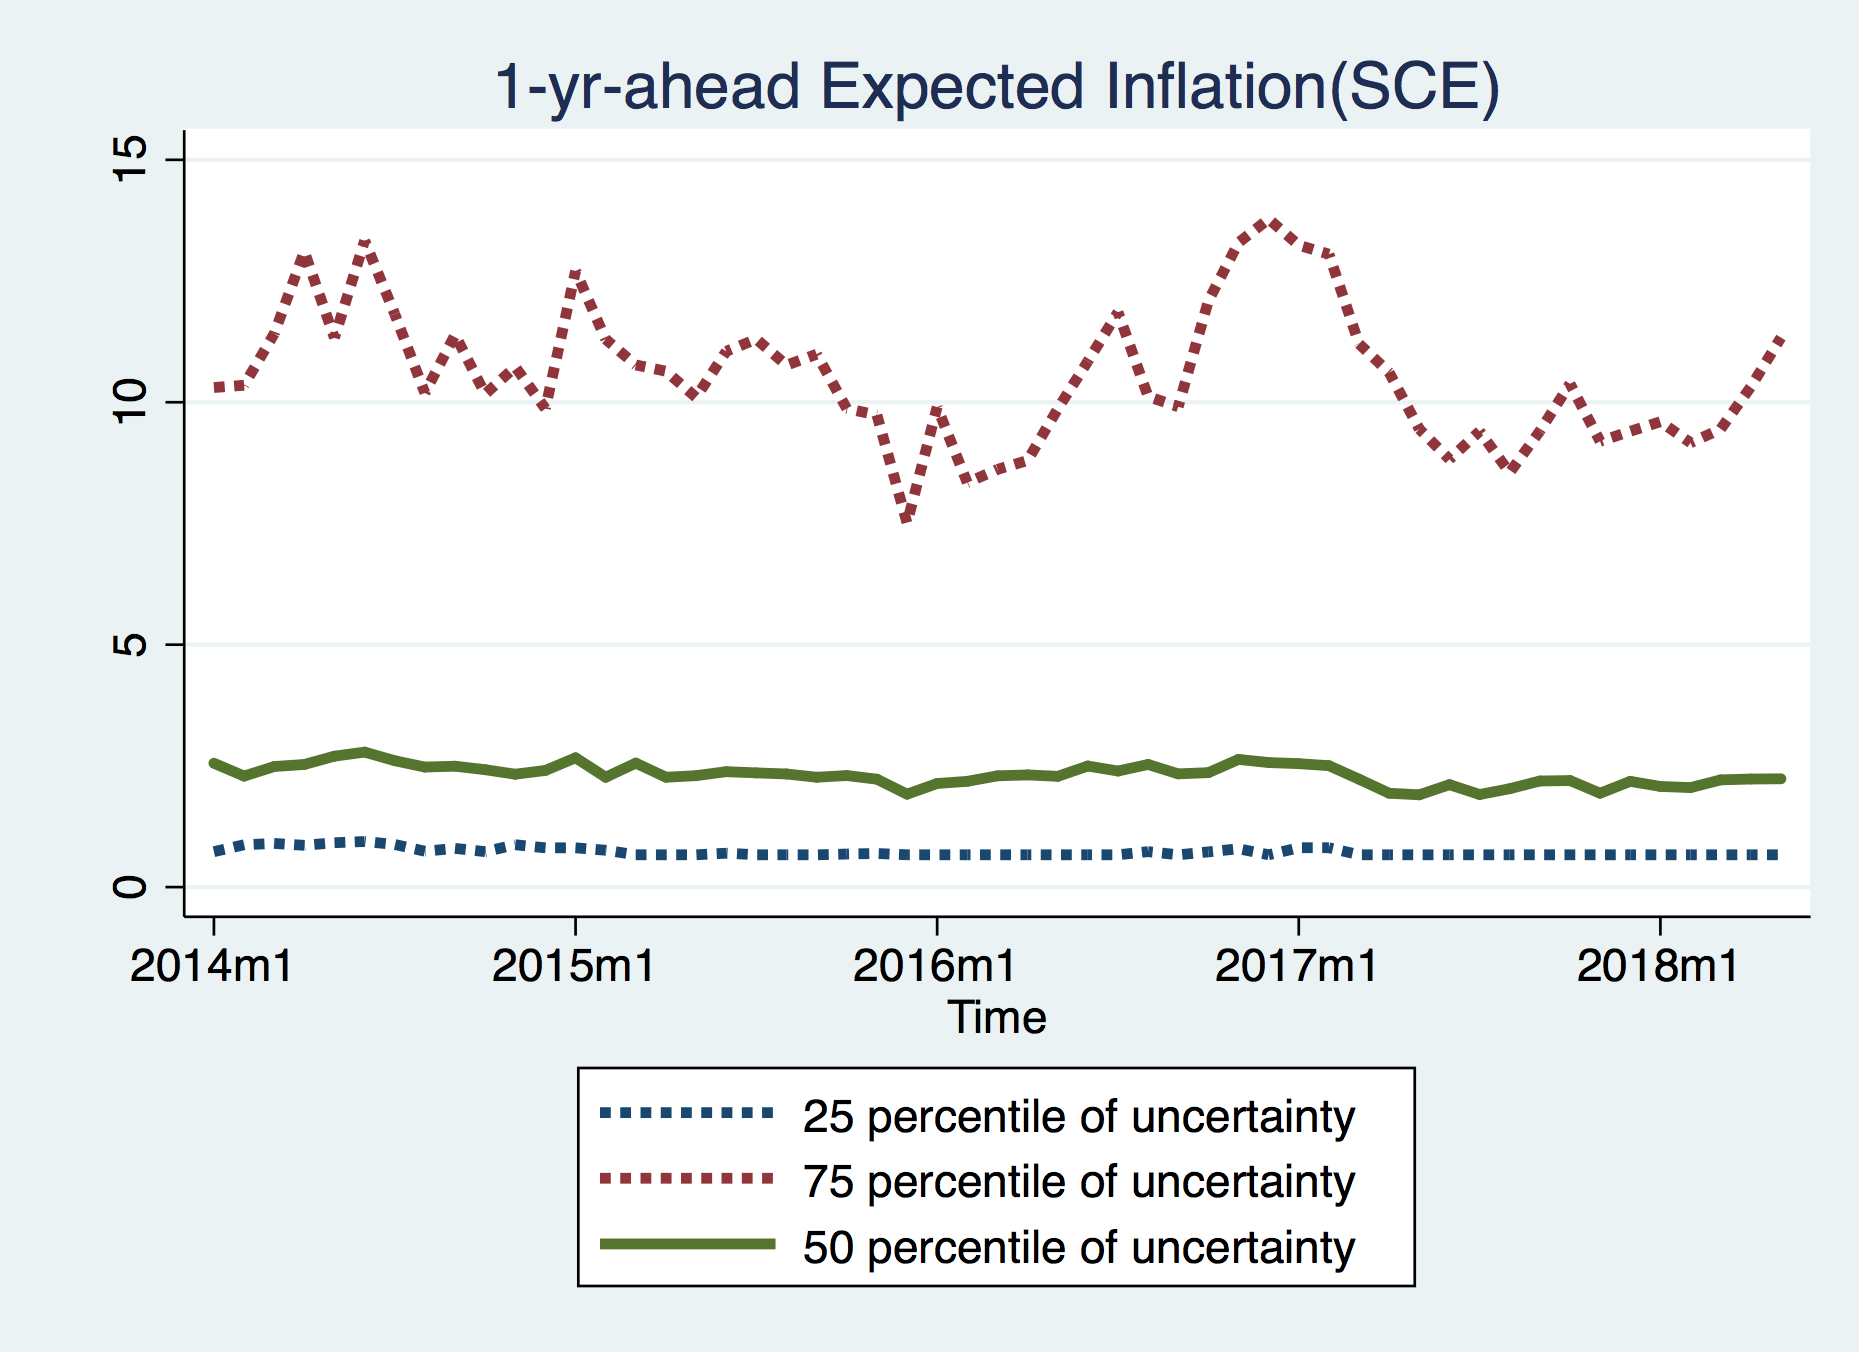
\includegraphics[width=7cm]{figures/IQRvarSCEM.png}
		\end{subfigure}
		\caption{Dispersion of Mean Forecasts and Unceratinty }
		\label{IQR_Unceratitny}
	\end{figure}
	
	
	\begin{figure}[ht]
		\begin{subfigure}[b]{0.5\textwidth}
		\centering
		\caption{Revision in Mean Forecasts}
		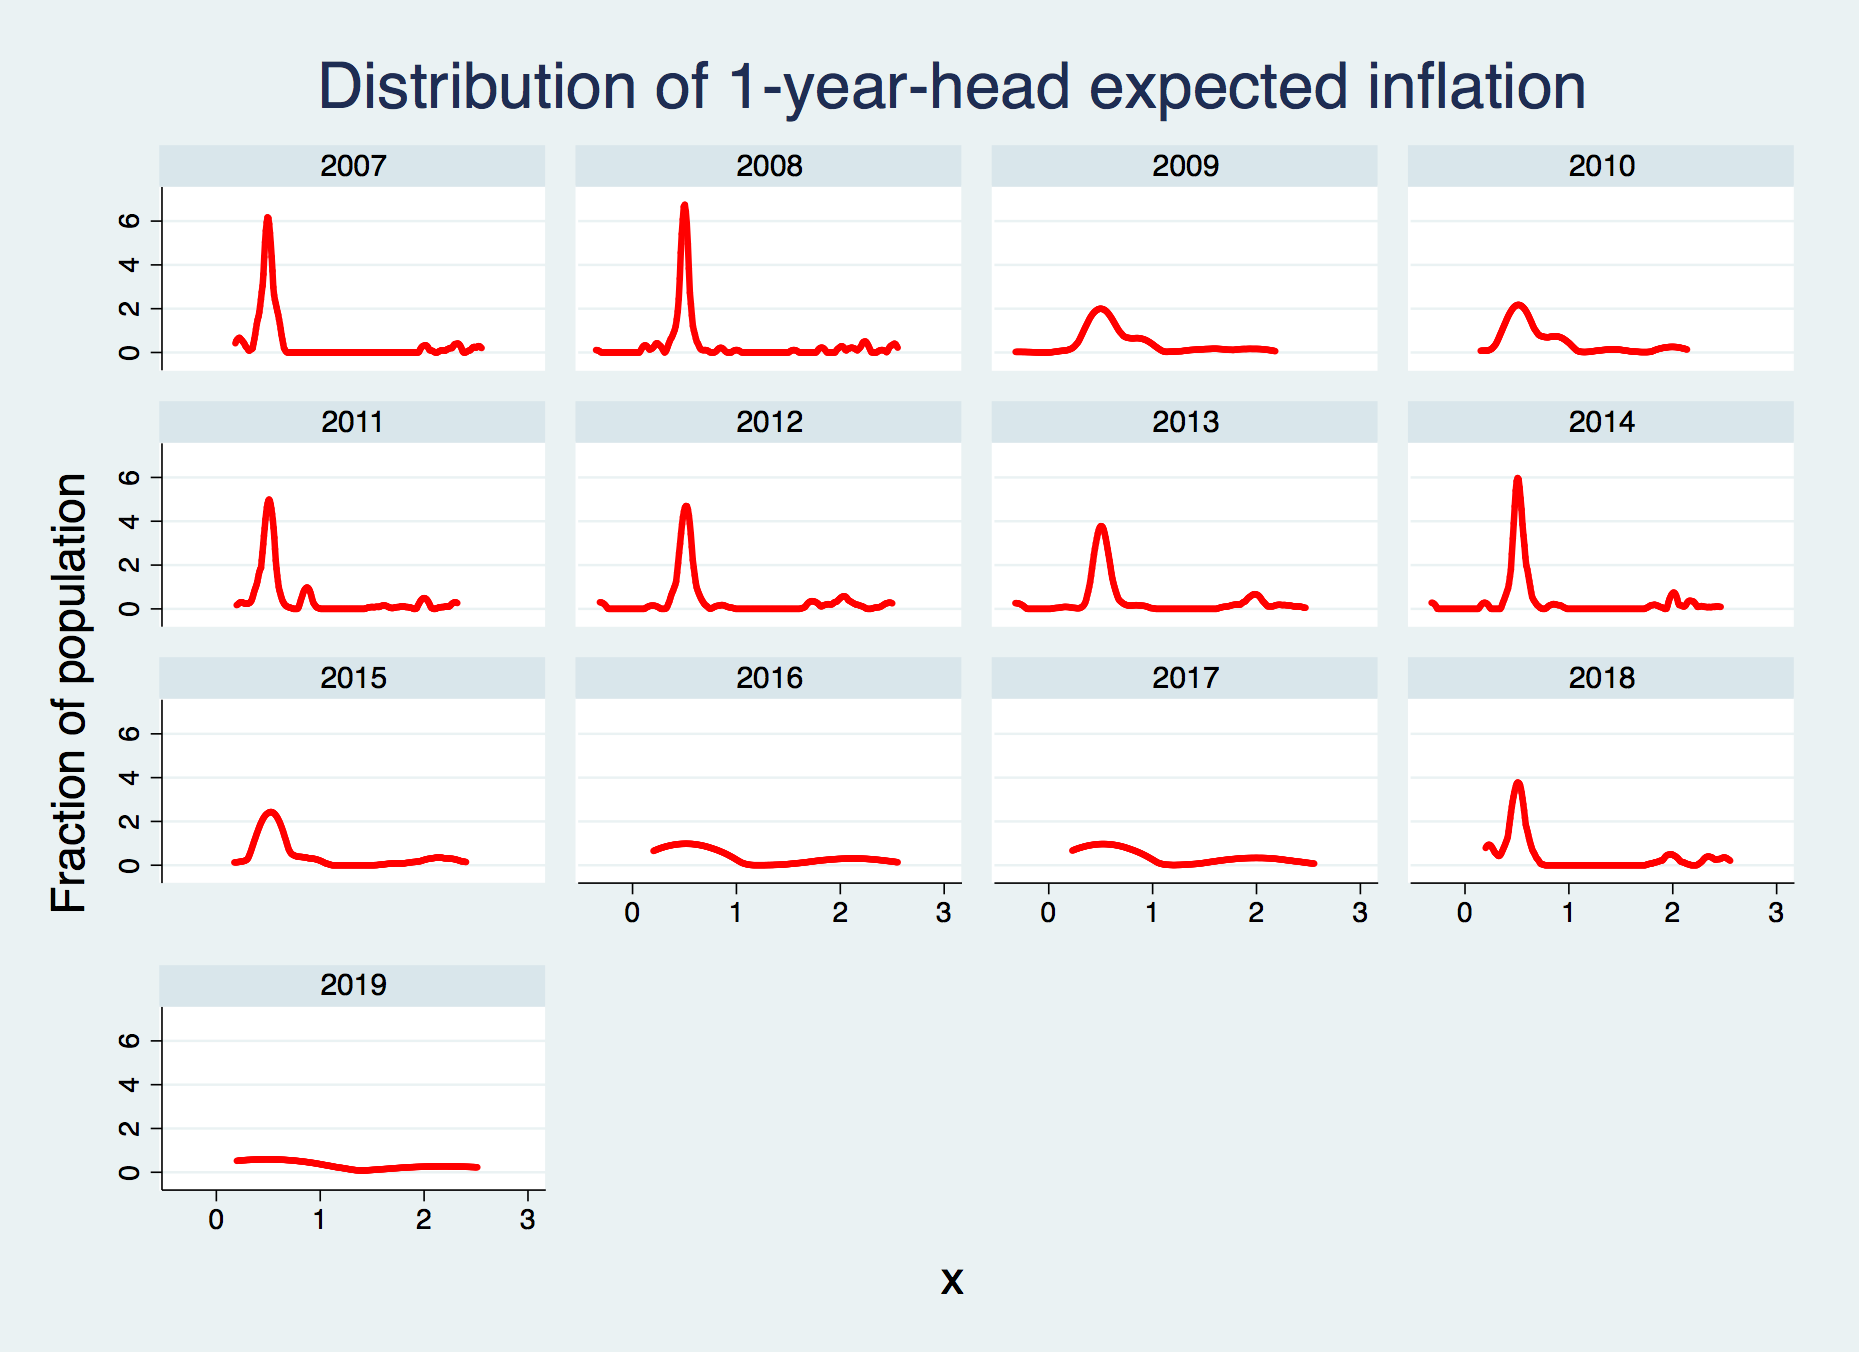
\includegraphics[width=7cm]{figures/PRCCPIMean1_hist.png} 
		\smallskip
		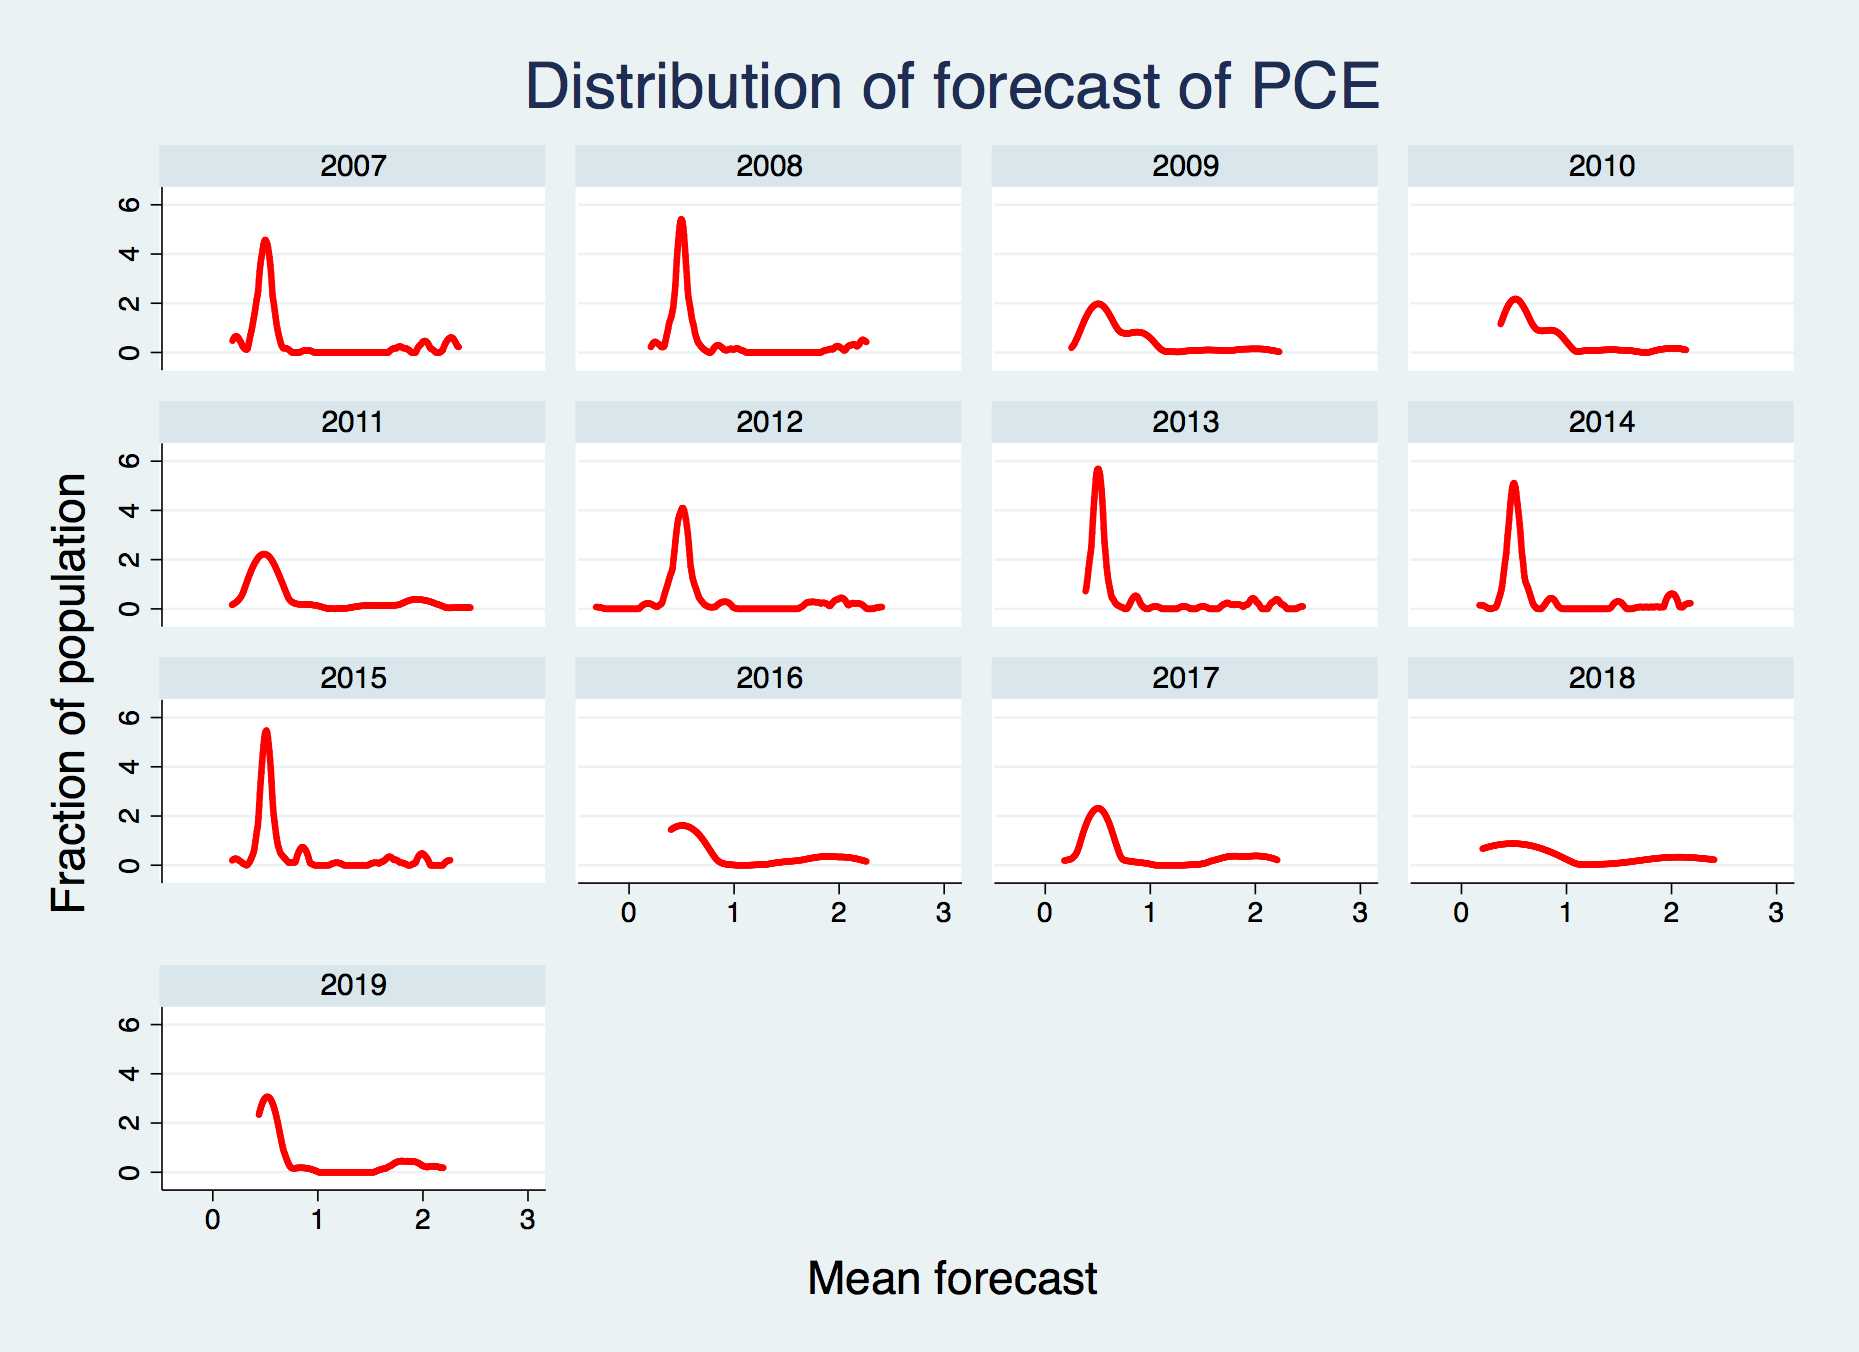
\includegraphics[width=7cm]{figures/PRCPCEMean1_hist.png} 
		\smallskip
		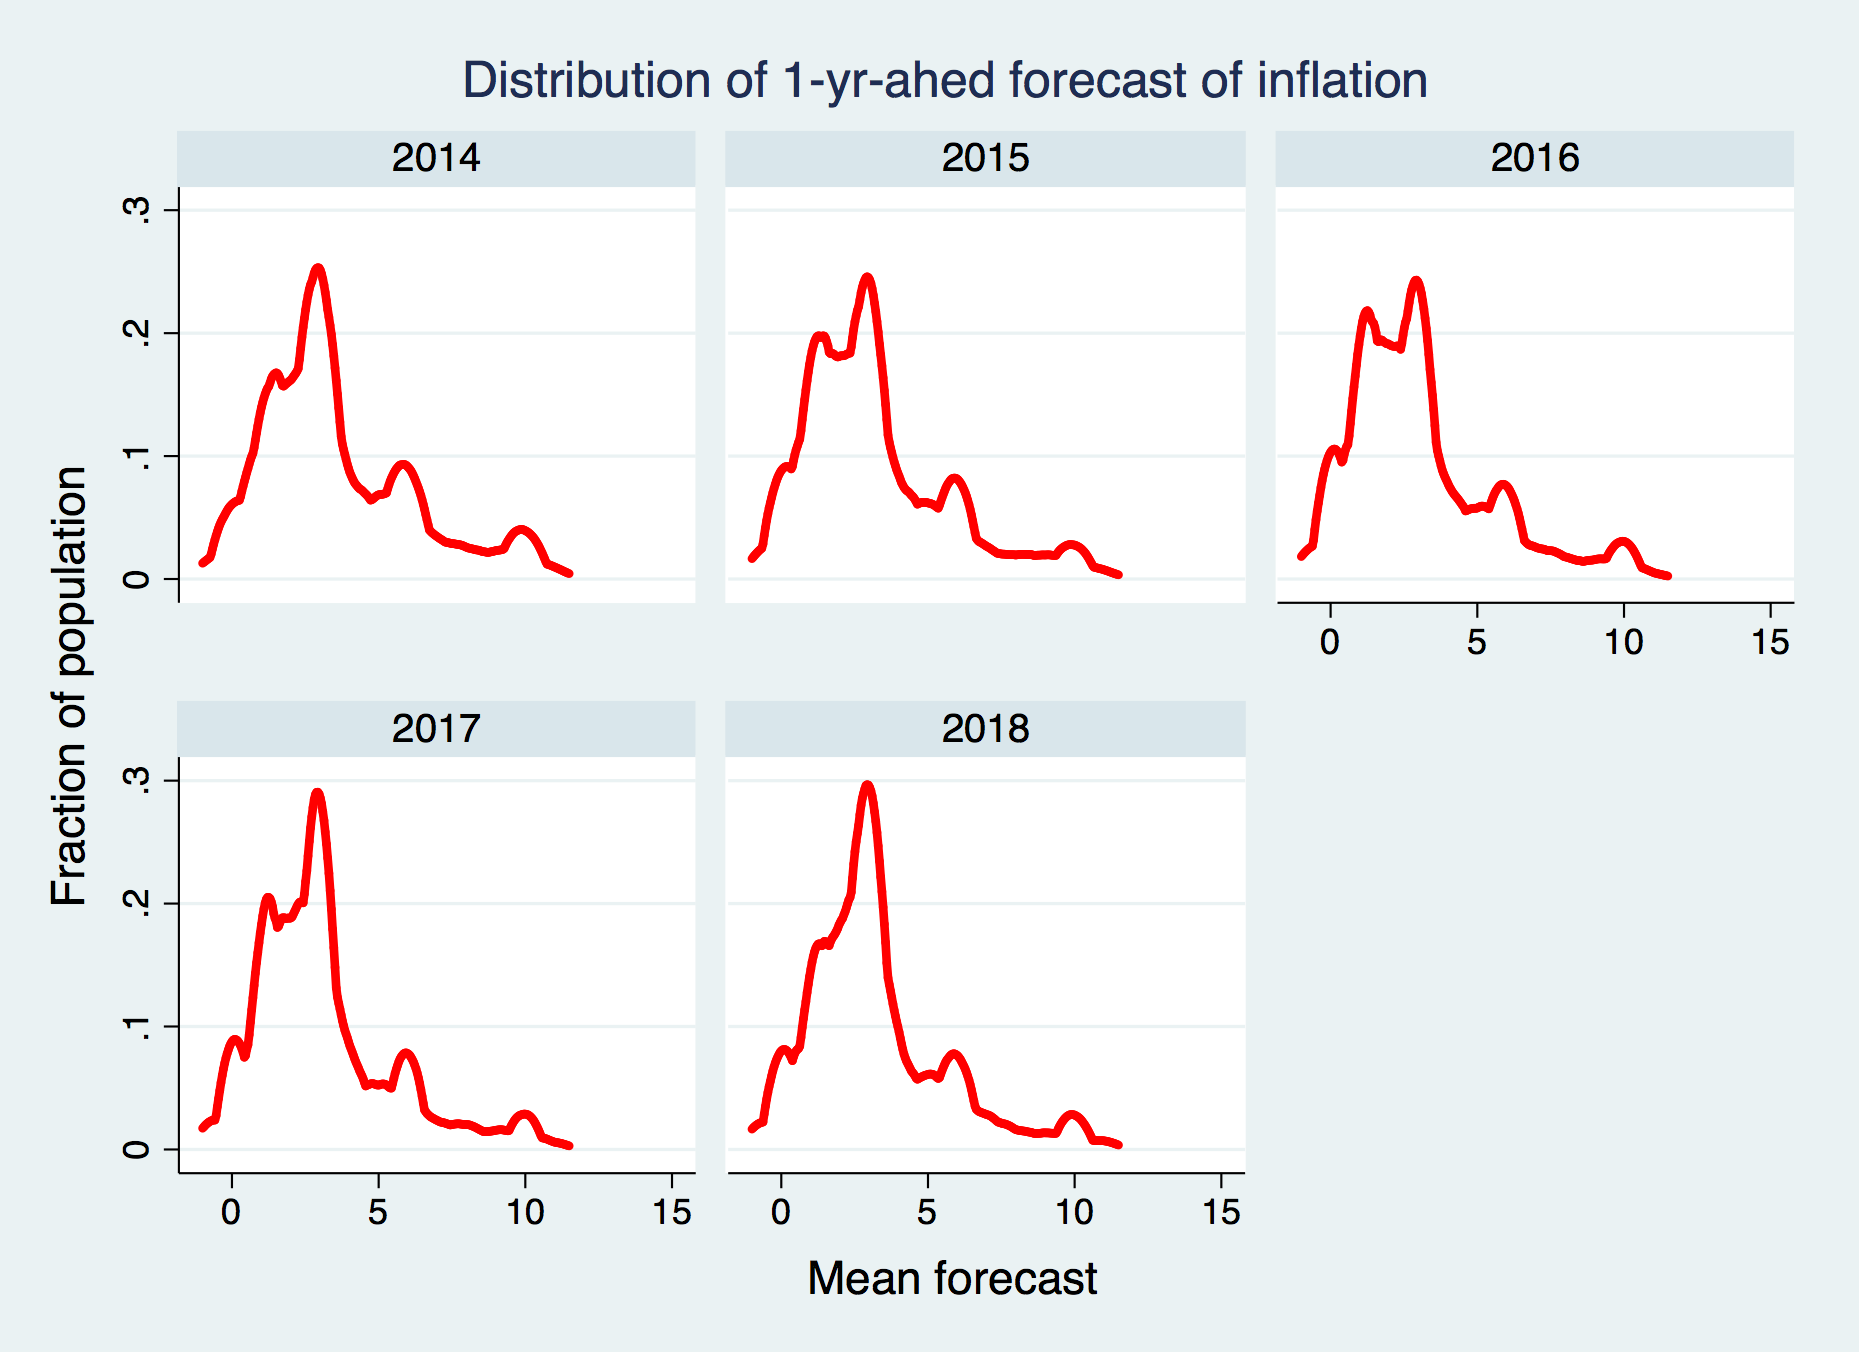
\includegraphics[width=7cm]{figures/SCEmean_hist.png} 
		\end{subfigure}
	   \hfill 
	  	\begin{subfigure}[b]{0.5\textwidth}
	  	\caption{Revision in Uncertainty}
		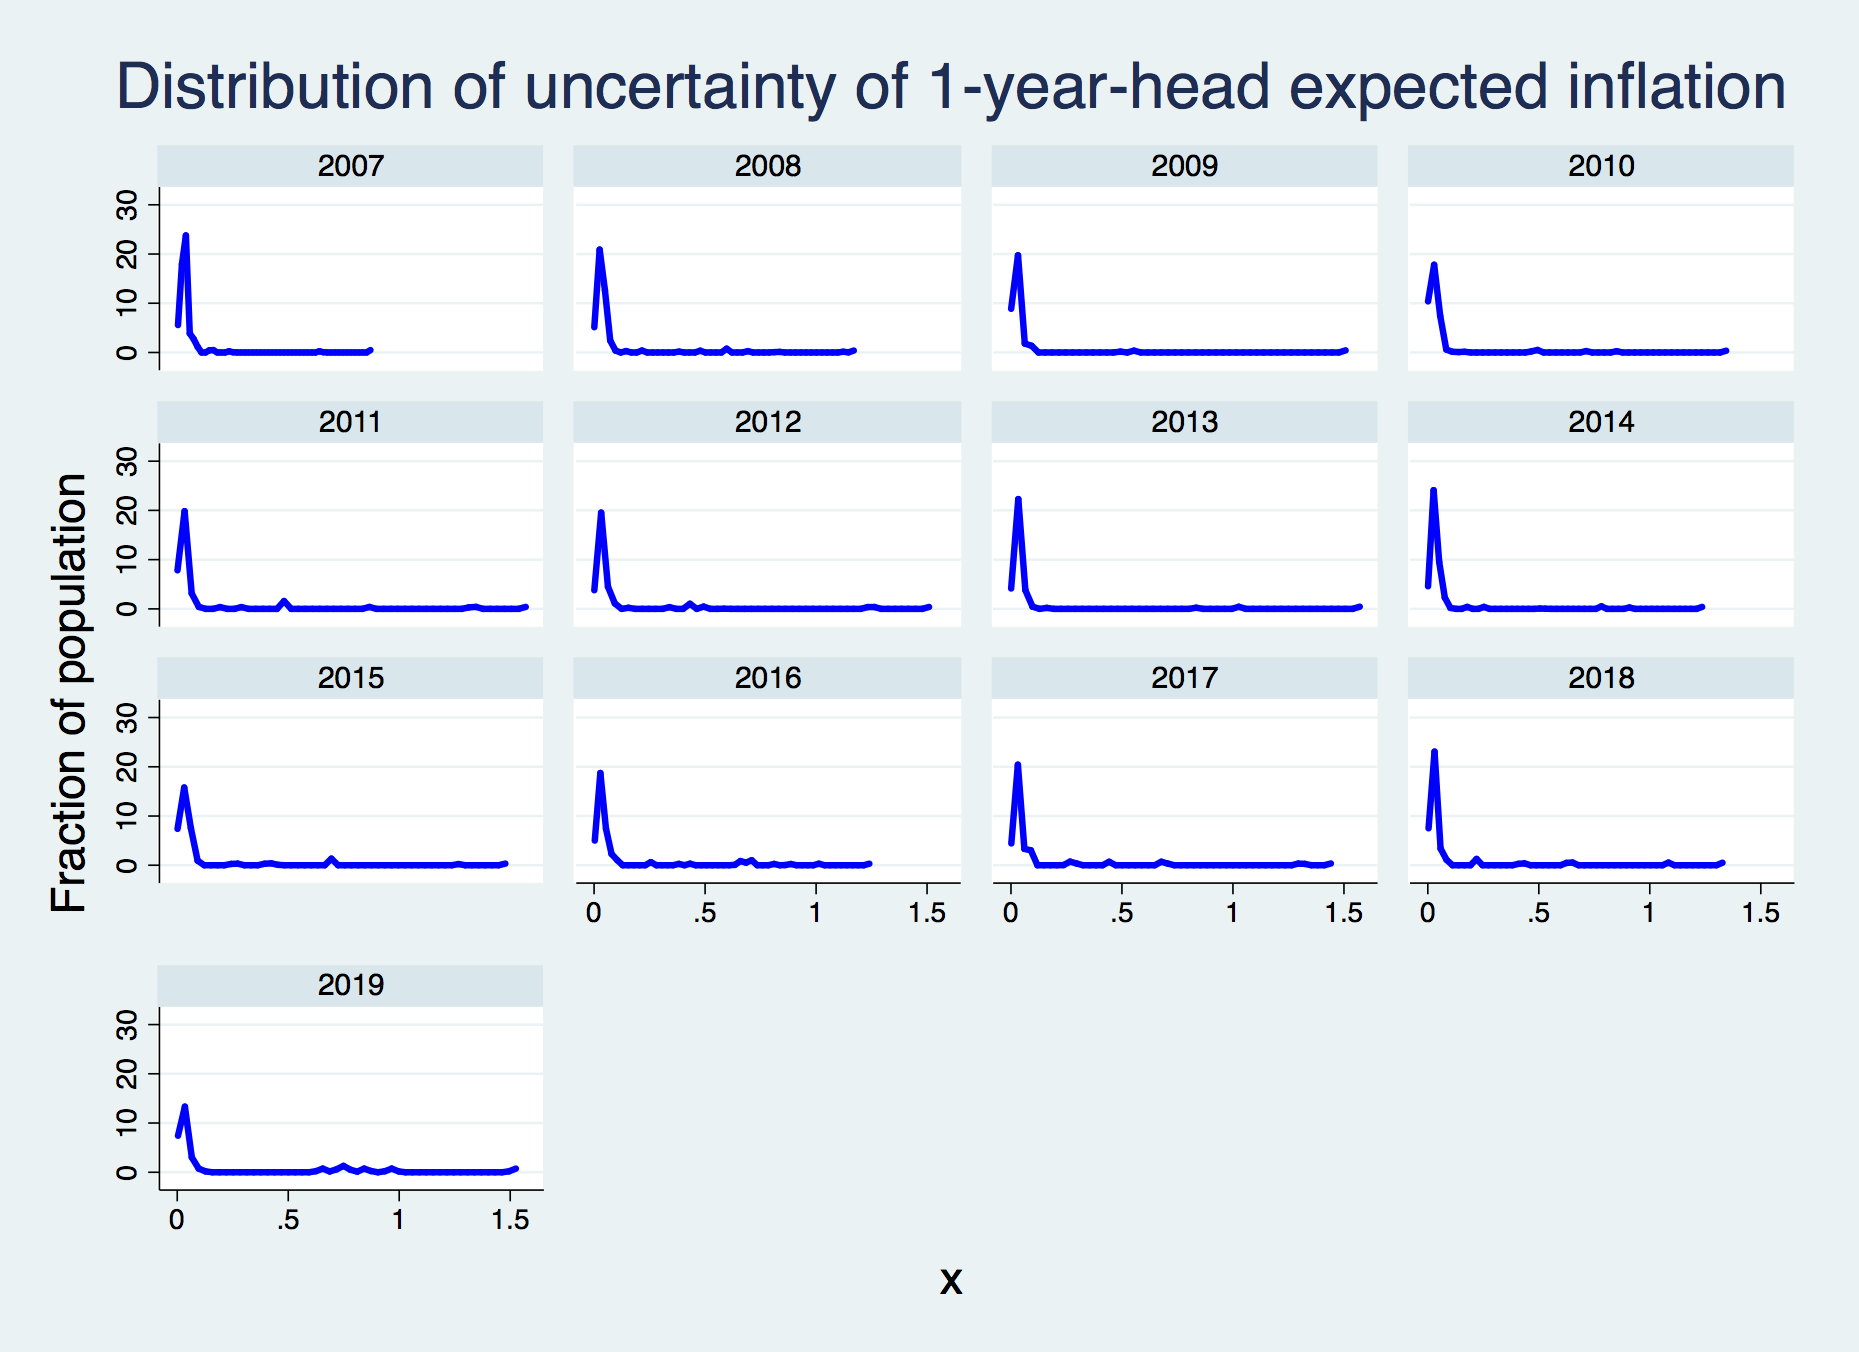
\includegraphics[width=7cm]{figures/PRCCPIVar1_hist.png}  
		\smallskip
		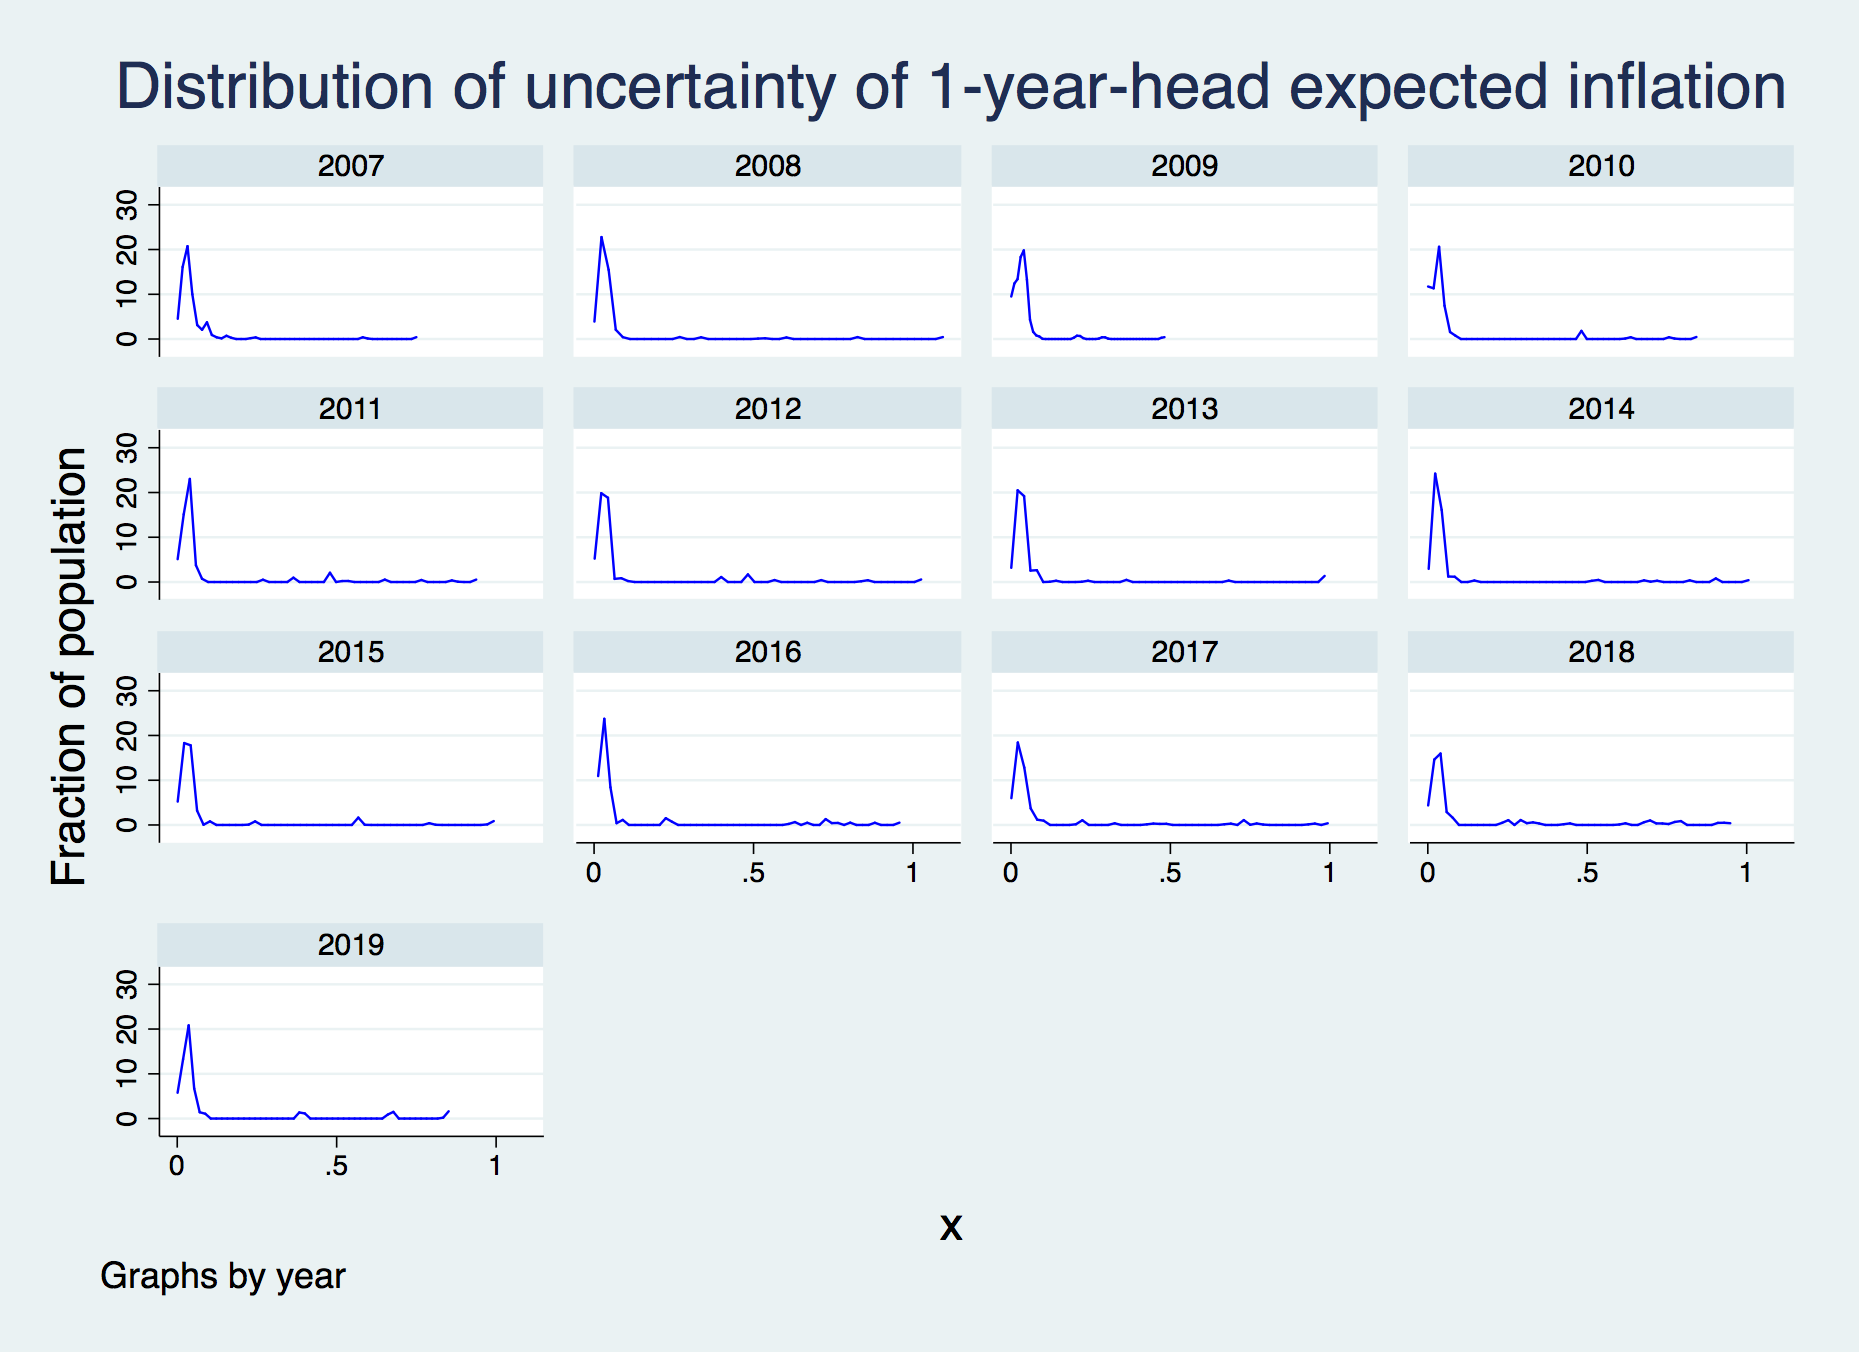
\includegraphics[width=7cm]{figures/PRCPCEVar1_hist.png}  
		\smallskip
		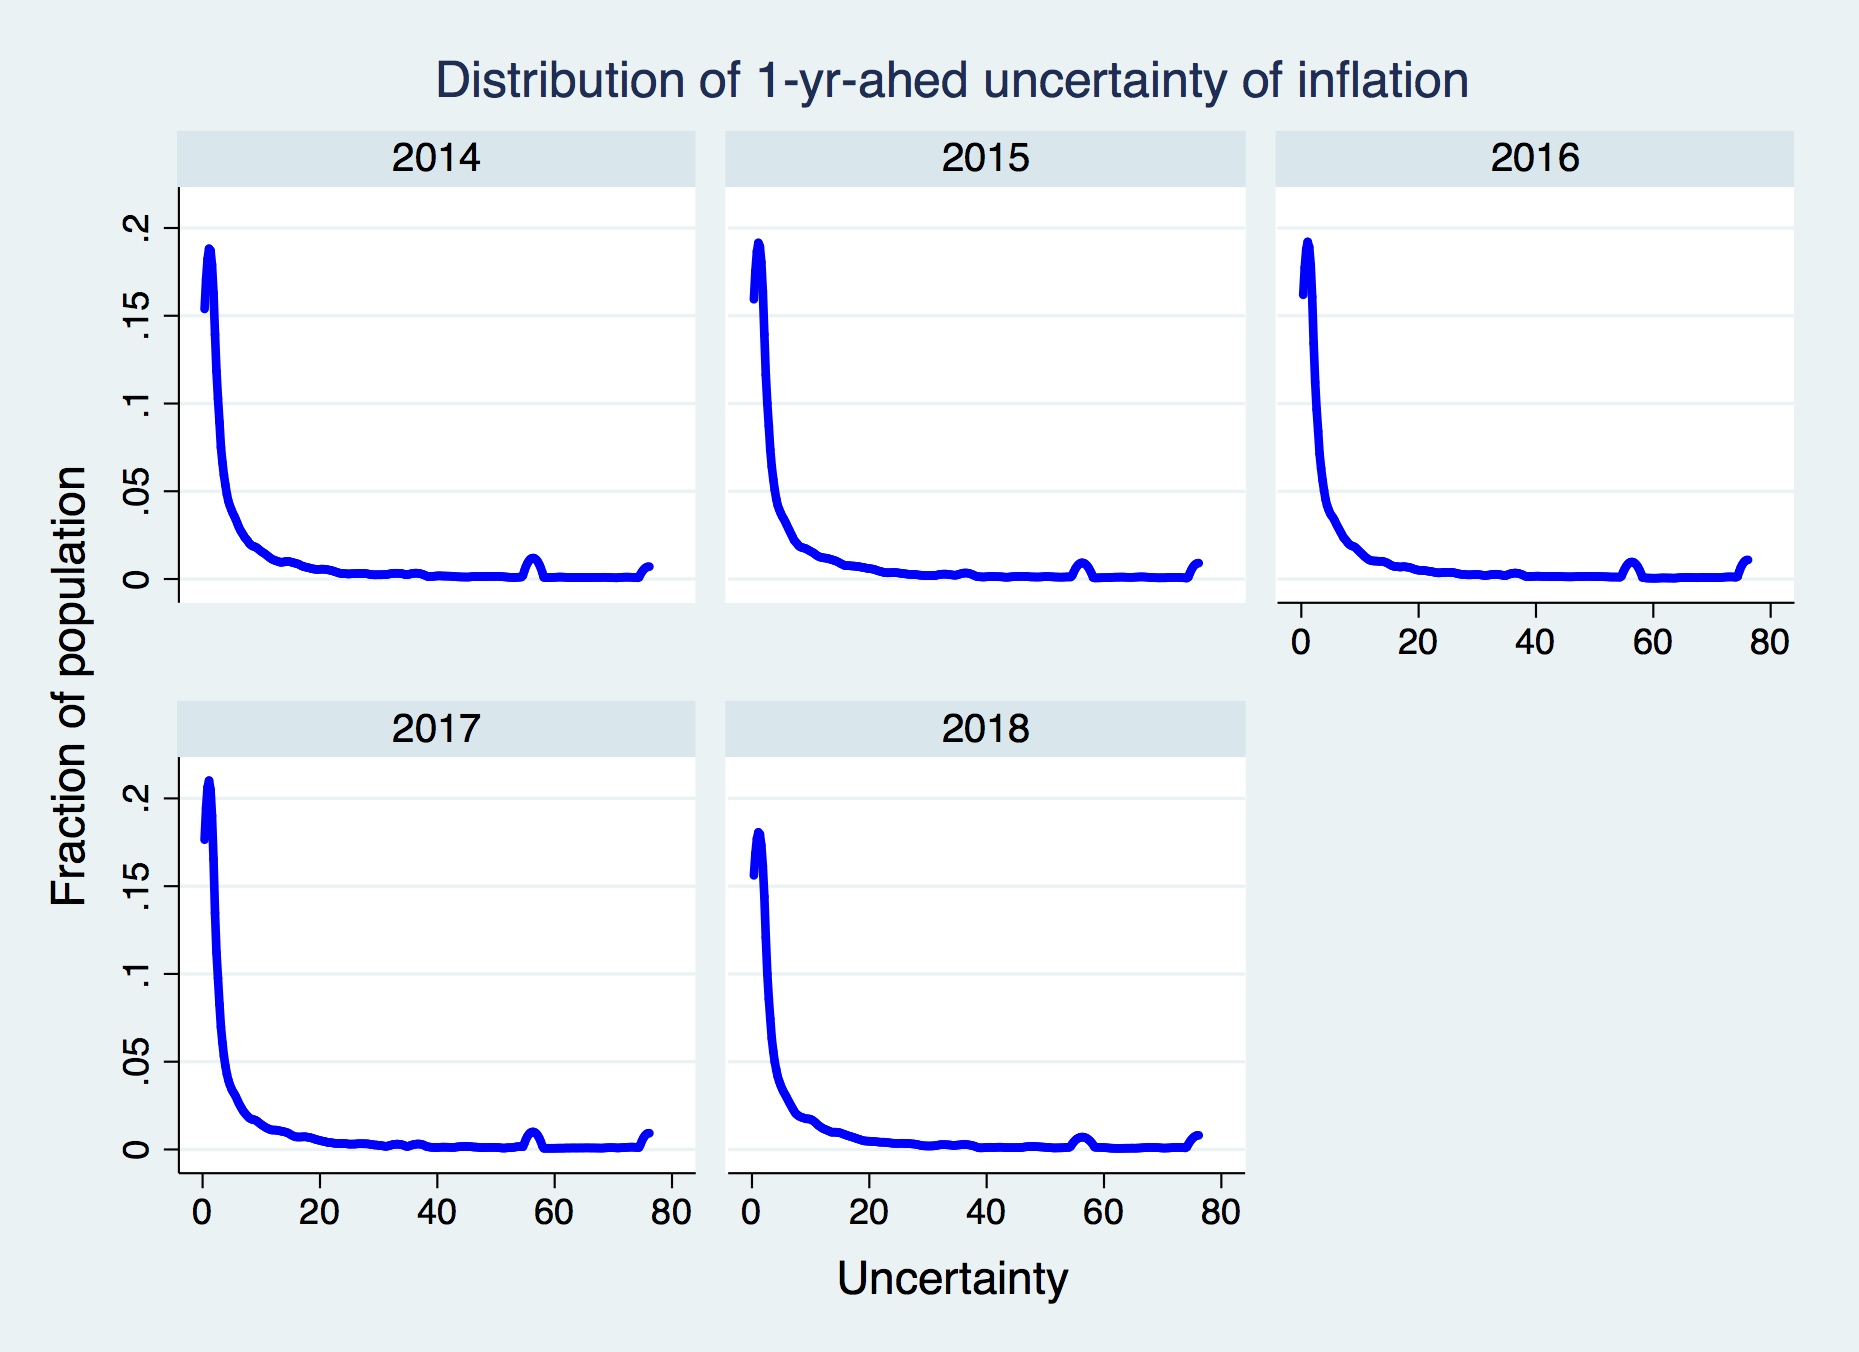
\includegraphics[width=7cm]{figures/SCEvar_hist.png}  
		\end{subfigure}
		\caption{Distribution of Mean Forecast and Uncertainty }
		\label{Unceratitny_Histogram}
	\end{figure}
	
	
	\begin{figure}[ht]
		\begin{subfigure}[b]{0.5\textwidth}
		\centering
		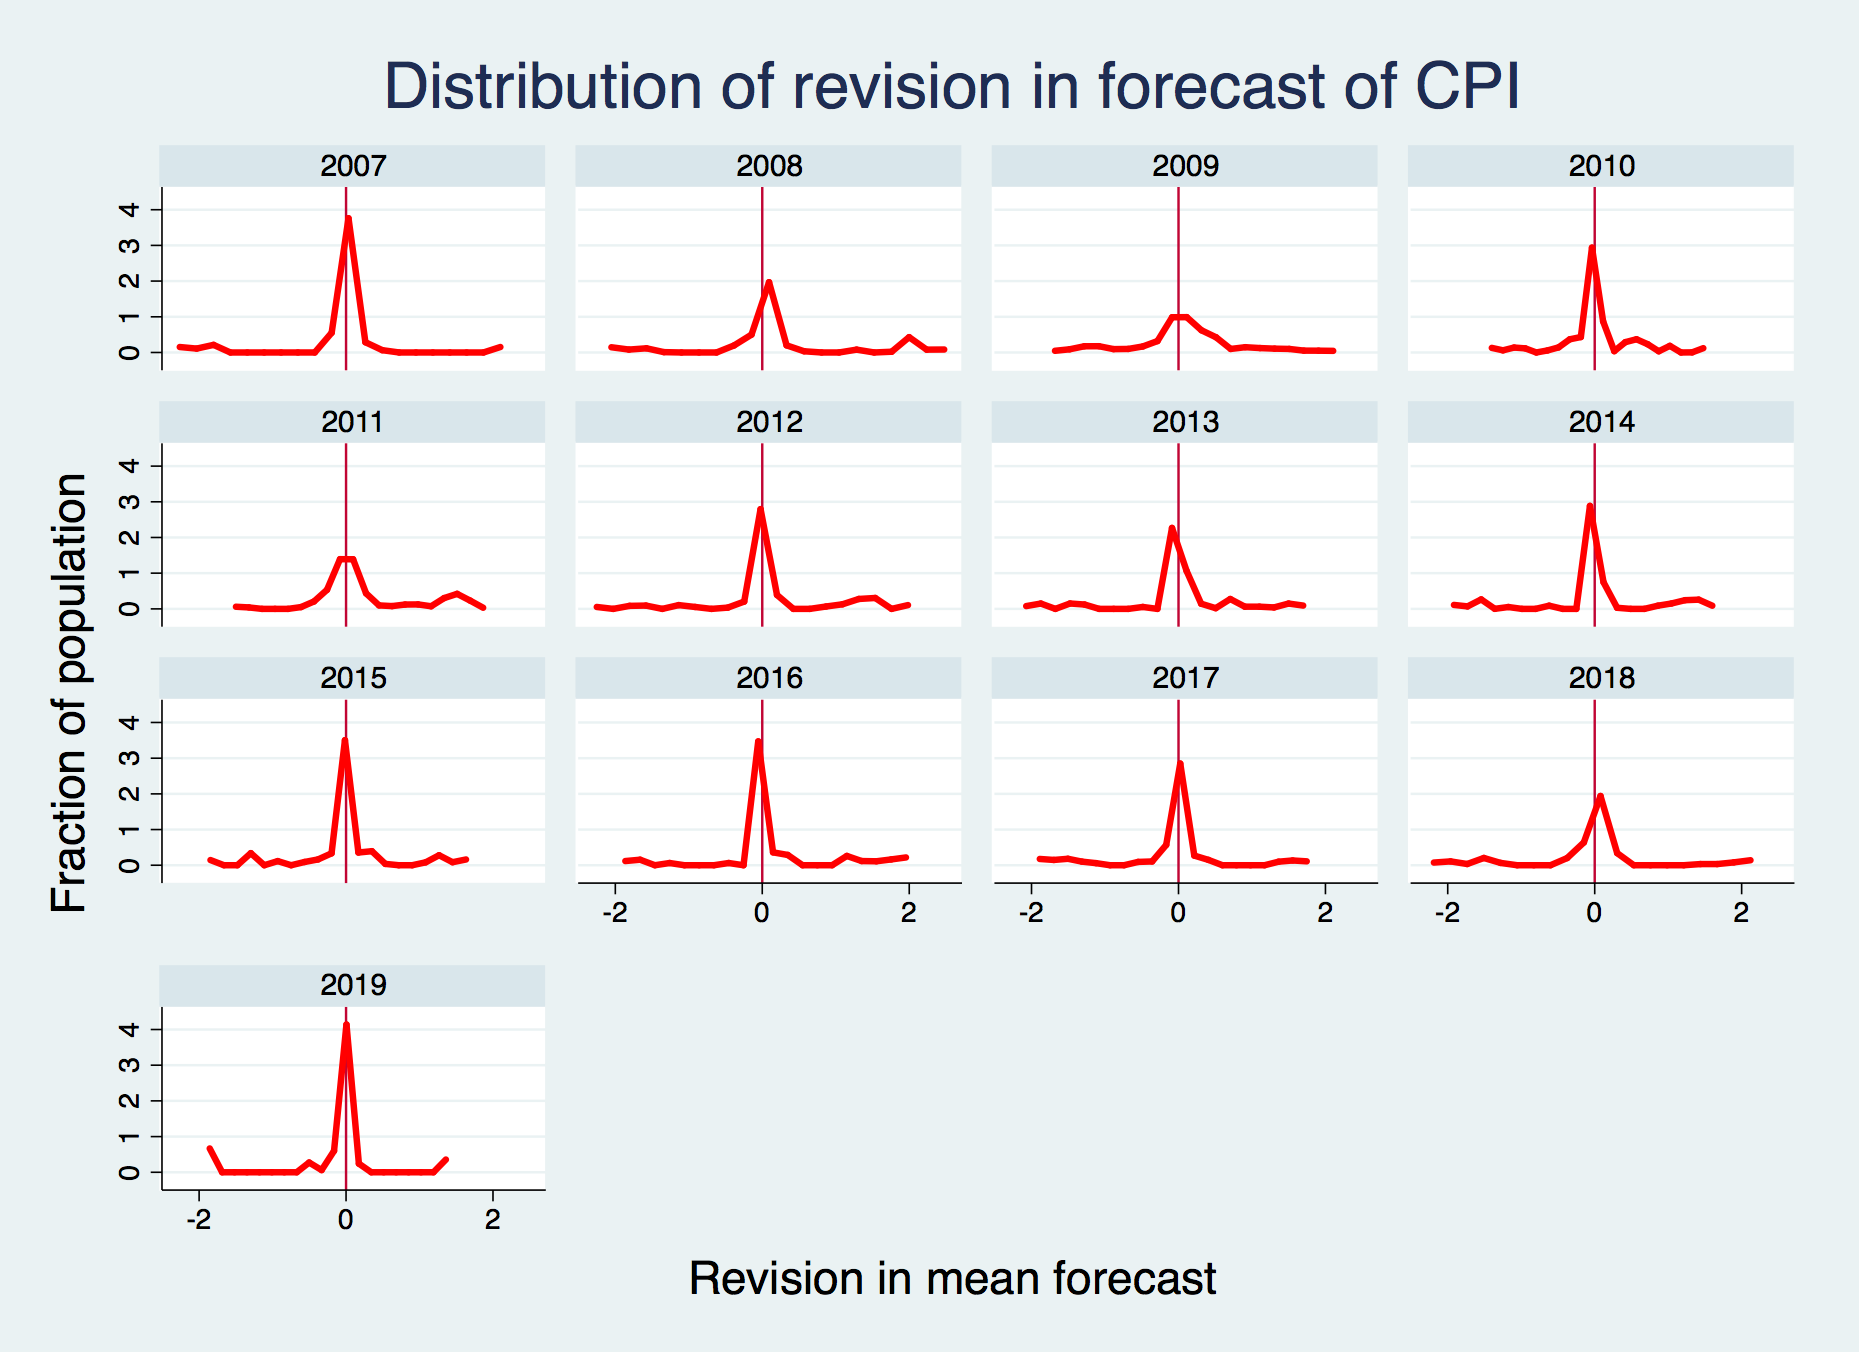
\includegraphics[width=7cm]{figures/PRCCPIMean01_rv_true_hist.png} 
		\smallskip
		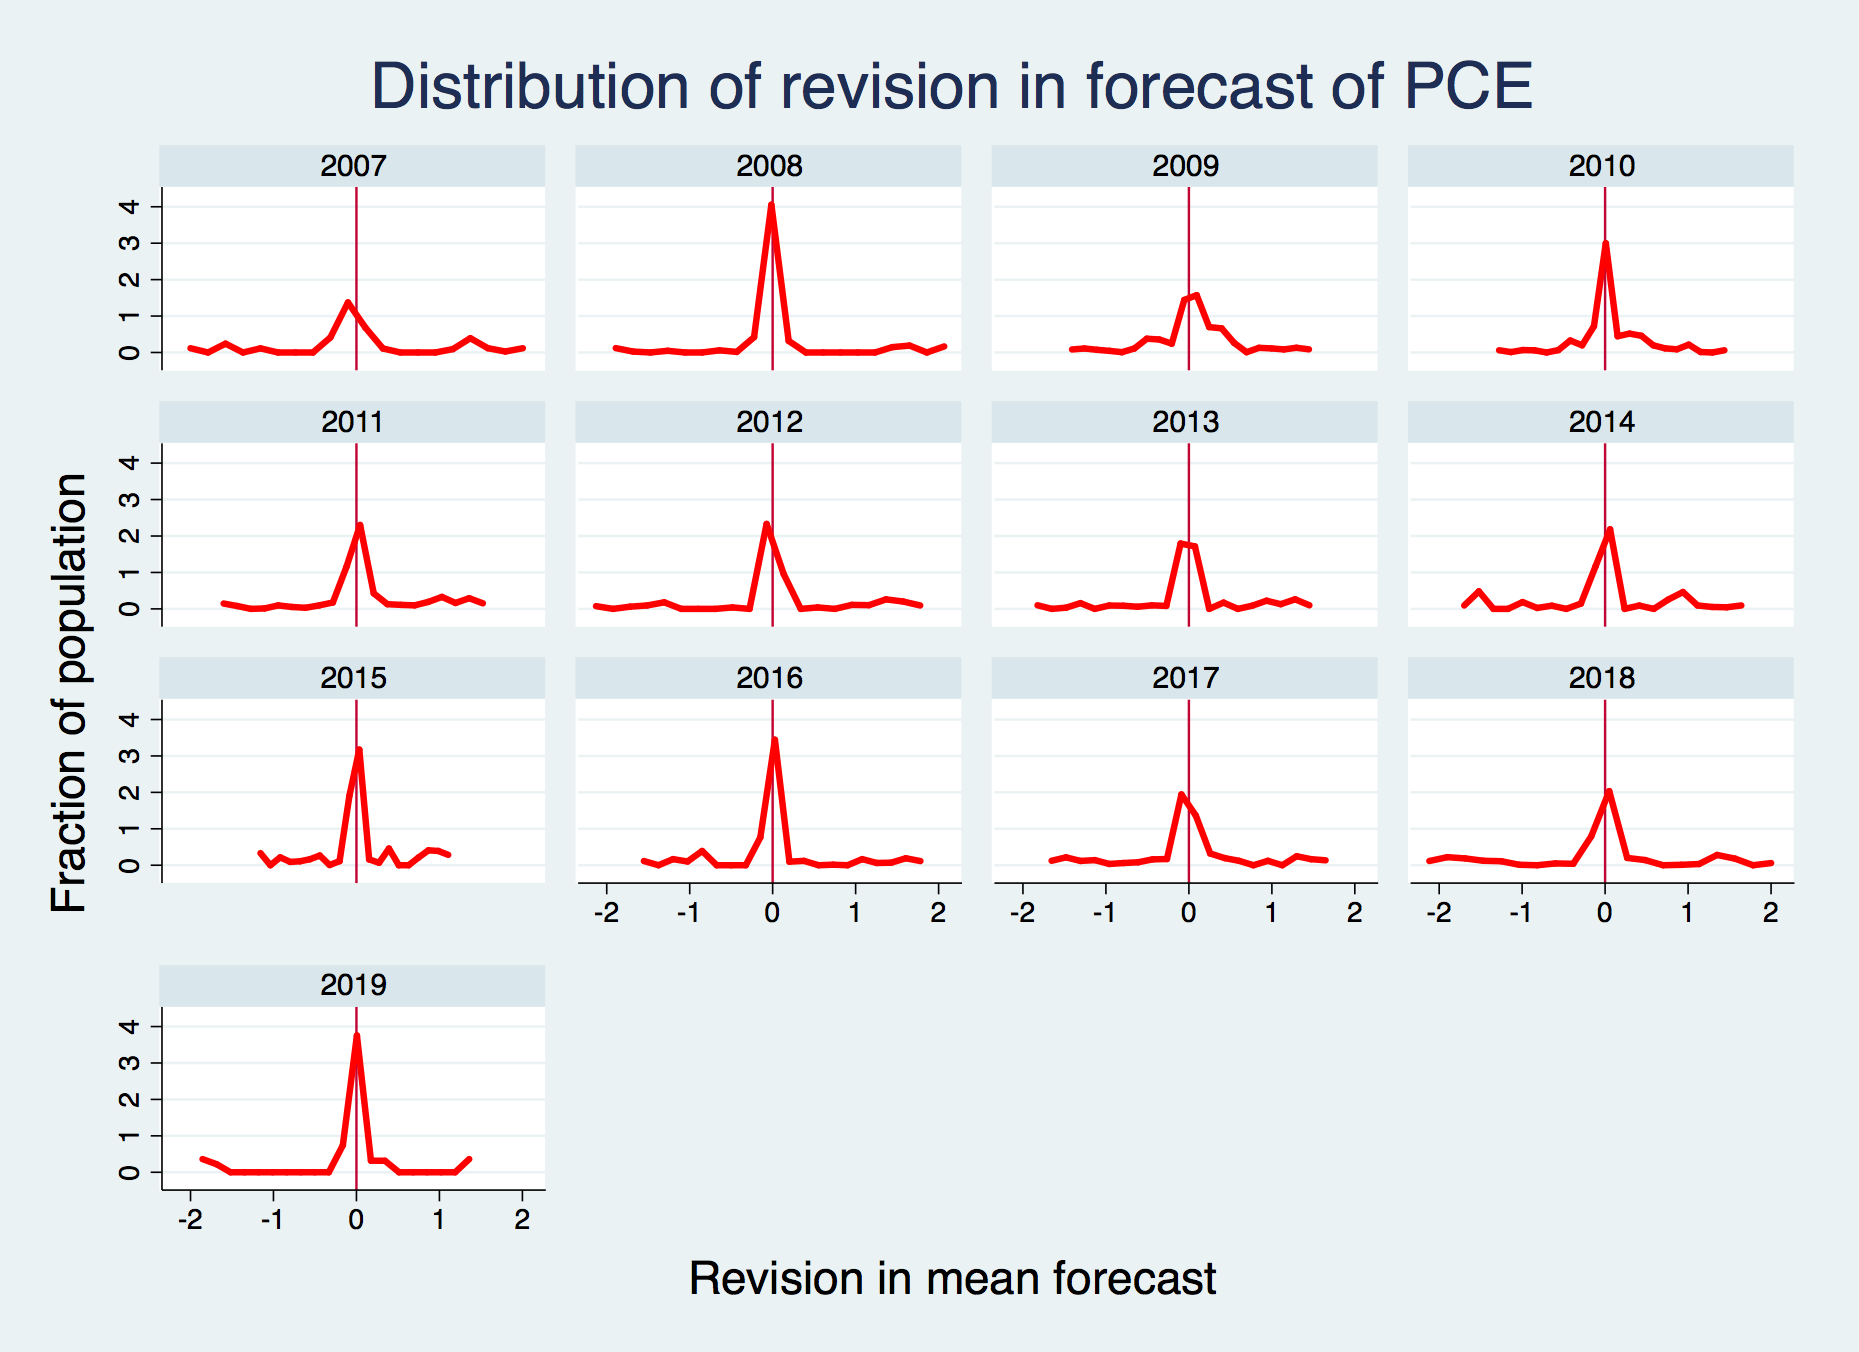
\includegraphics[width=7cm]{figures/PRCPCEMean01_rv_true_hist.png} 
		\end{subfigure}
		   \hfill 
		\begin{subfigure}[b]{0.5\textwidth}
		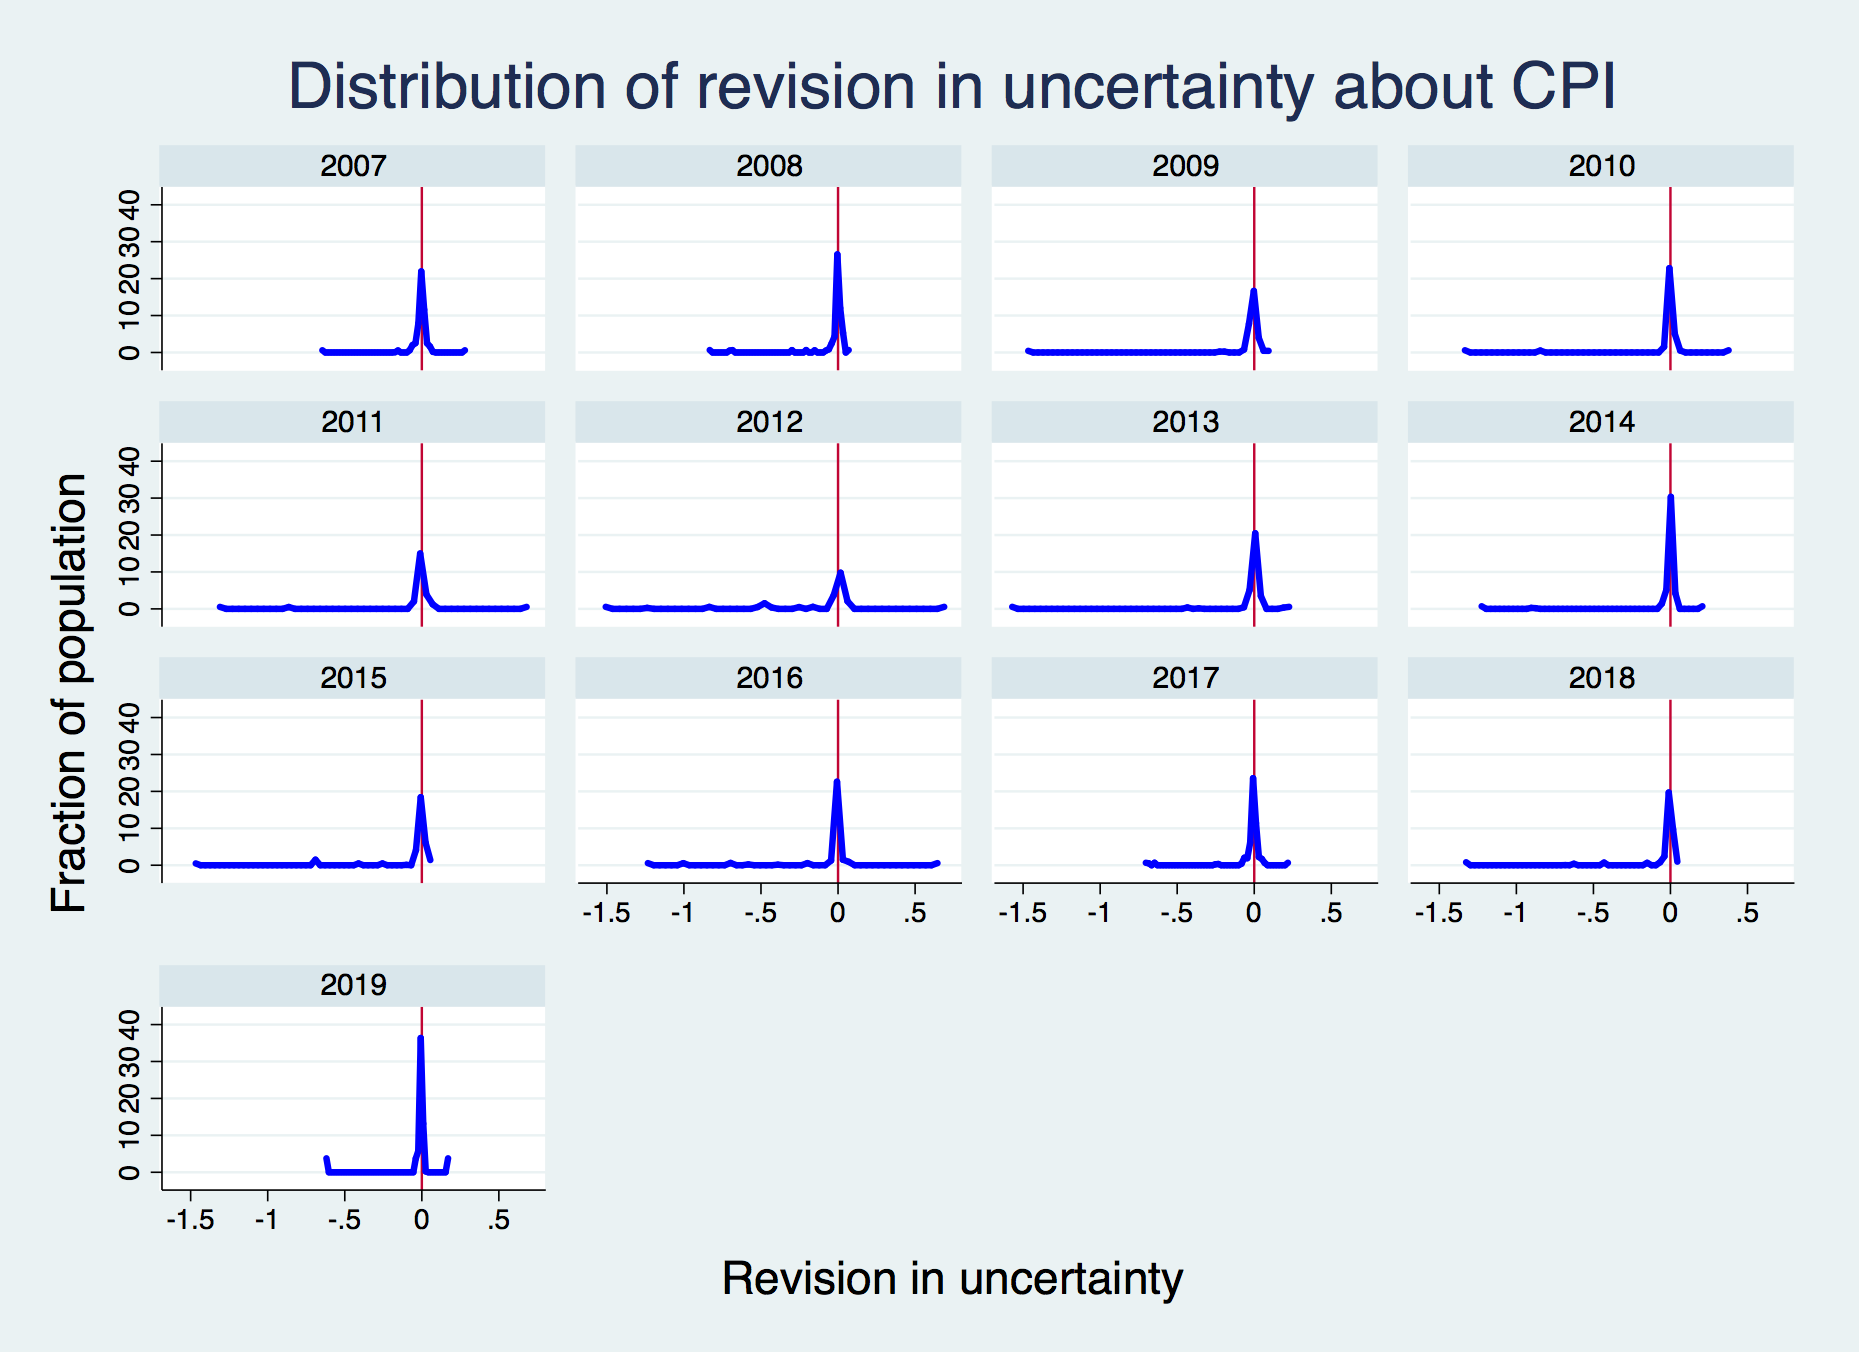
\includegraphics[width=7cm]{figures/PRCCPIVar01_rv_true_hist.png}  
		\smallskip
		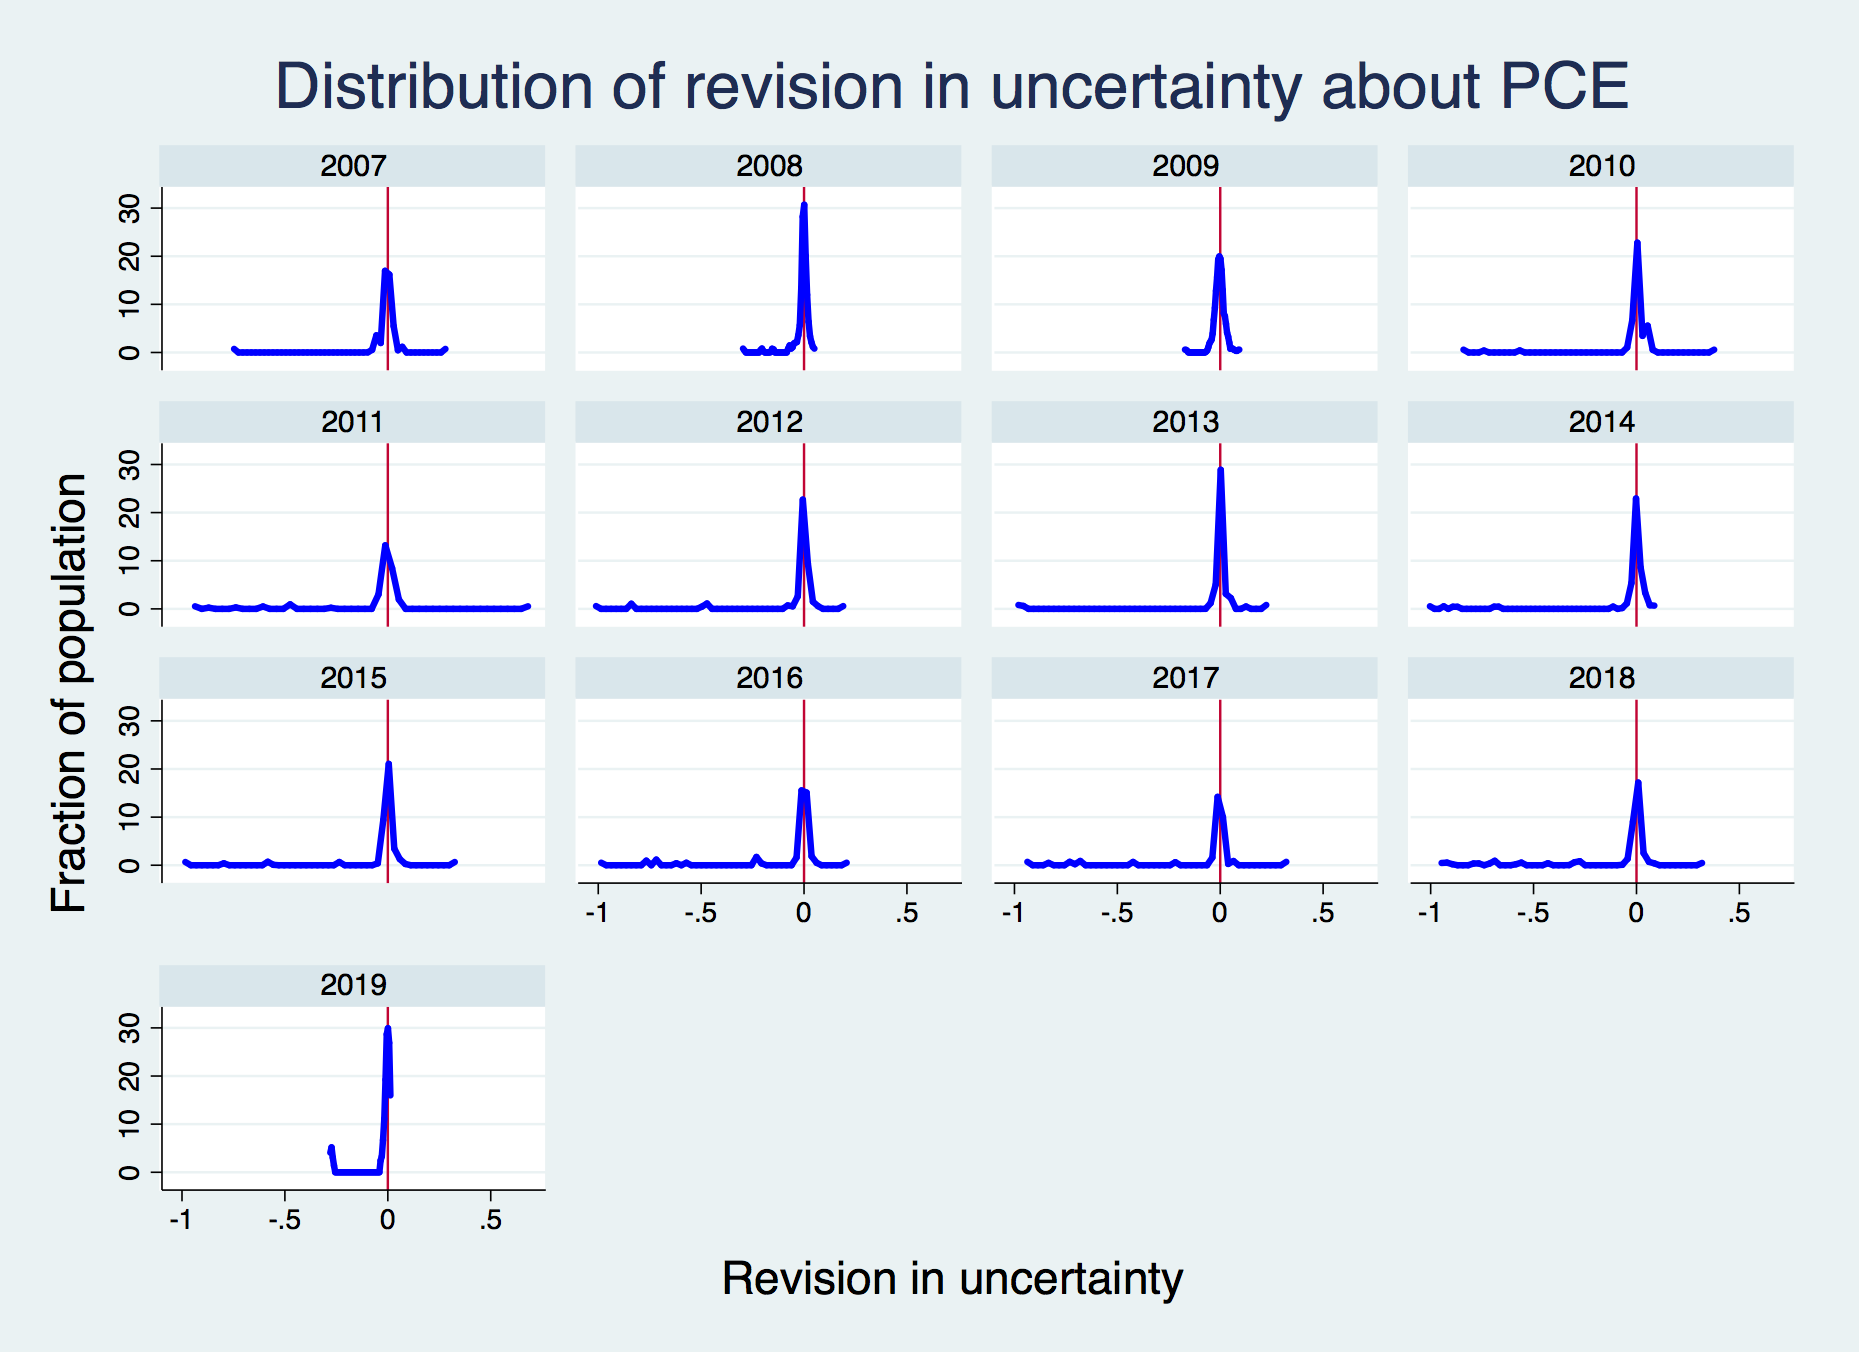
\includegraphics[width=7cm]{figures/PRCPCEVar01_rv_true_hist.png} 
		\end{subfigure}
		\caption{Distribution of Revision in Forecasts and Uncertainty}
		\label{RevisionHist}
	\end{figure}
	
	
	\subsection{Test of null hypothesis of rational expectation}\label{NullTest}
	
	This section first reproduces a number of statistical tests of FIRE used seen existing literature in Table \ref{NullTestTable}, primarily following \citet{mankiw2003disagreement},  and then extends the tests relying on uncertainty in Table \ref{RevEfficiency} and \ref{WeakRevEfficiency}, in the spirit of forecasting efficiency by \citet{nordhaus1987forecasting}. It is an extension of what \citet{fuhrer2018intrinsic} does to mean forecast to uncertainty.  
	
	The first set of tests, hereafter, referred to as FE-based tests, utilize the moment restrictions on forecast errors. In plain words, the null hypotheses of the three tests are the following. First, since the forecasts are on average unbiased according to FIRE, forecast errors across agents should converge to zero in a large sample. Second, forecast errors of non-overlapping forecasting horizon are not serially correlated (Equation \ref{NoSerialCorrFE} ).  Third, forecast errors cannot be predicted by any information available at the time of the forecast, including the mean forecast itself and other variables that are in the agent's information set. This follows from Equation \ref{NoPastInfFE}. In addition, I include what is called weak version of the FE-based test which explores the serial correlation of forecast errors in overlapping periods,  i.e. 1-year-ahead forecasts within one year. The forecast errors are correlated to the extent of the realized shocks in the overlapping periods. So the positive serial correlation does not directly violates FIRE. But the correlation of overlapping forecast errors still contain the useful information about the size of the realized shocks. 
	
	FE-based tests results are presented in Table \ref{NullTestTable}. Individual level data are used thanks to the panel structure of both surveys. Since test 2 and 3 requires individual forecasts in vintages that are more than one year apart while SCE only surveys each household for 12 months, the two tests are done for only SPF forecasts of CPI and PCE. Also, the regressions are adjusted accordingly depending on the quarterly and monthly frequency of SPF and SCE. Since these regressions are based on 1-year inflations in overlapping periods, white standard error is computed for hypothesis testing. 
	
	First,  all three forecast series easily reject the unbiasedness test at the significance level of $1\%$. There is upward bias across professional forecasters and households \footnote{\citet{coibion2018firms} finds the same upward bias for firms' managers.}, while unsurprisingly, the bias is almost 20 times of that for professional forecasters(2.2 versus 0.12) for headline CPI. 
	
	Second, the point forecast one year ago predicts the forecast errors for professionals in the significance level of 1\%. For headline CPI inflation, for instance, one percentage point inflation forecast corresponds to 0.3 percentage points of the forecast errors one year later. Thus test 2 in Table \ref{NullTestTable} easily rejects the second hypothesis test of FIRE that past information does not predict future forecast errors. 
	
	Third, forecast errors can be predicted by forecast errors one year ago with a significant coefficient of around $0.08$ for headline CPI and $0.05$ for PCE, as seen in test 3 of Table \ref{NullTestTable}. Errors of non-overlapping forecasting periods are correlated, against the null of FIRE. 
	
	Lastly, test 4 in Table \ref{NullTestTable} presents a higher serial correlation of forecast errors produced within a year. For SPF forecasts, the serial correlation does not exist beyond 1 quarter, implying relative efficiency of forecasts. For the households, the forecast errors are more persistent over the entire year in that current forecast errors are correlated with all past forecast errors over the past three quarters.  Again, although the persistence of 1-year forecast errors within one year does not directly violate FIRE, the fact that households' forecast errors being more persistent than professionals provide useful clues about the relative rigidity of the two types of agents. 
	
	\begin{table}[ht]
		\caption{Tests of Rationality and Efficiency using Forecast Errors}
		\label{NullTestTable}
		\centering 
		\begin{tabular}{llll}
			\hline 
			& SPF CPI          & SPF PCE          & SCE            \\
			\hline 
			\multicolumn{4}{l}{Test 1: Unbiasedness}                                                           \\
			\hline 
			Constant                            & 0.122***         & 0.586***         & 2.220***       \\
			& (0.017)          & (0.061)          & (0.019)        \\
			\hline 
			N                                   & 4697             & 1208             & 67380          \\
			\hline 
			\multicolumn{4}{l}{Test 2: FE does not depend on past information}                                  \\
			\hline 
			Forecast 1-yr before                & 0.307***         & 0.586***         & NA             \\
			& (0.020)          & (0.061)          & NA             \\
			Constant                            & -0.655***        & -0.777***        & NA             \\
			& (0.060)          & (0.116)          & NA             \\
			\hline 
			N                                   & 3429             & 1208             & NA             \\
			$R^2$                 & 0.0721           & 0.118            & NA             \\
			\hline 
			\multicolumn{4}{l}{Test 3: FEs of non-overlapping forecast horizons not serially correlated} \\
			\hline 
			Forecast Error 1-year before        & 0.0756***        & 0.0503***        & NA             \\
			& (0.020)          & (0.035)          & NA             \\
			Constant                            & 0.145***         & 0.275***         & NA             \\
			& (0.021)          & (0.035)          & NA             \\
			\hline 
			N                                   & 3356             & 1208             & NA             \\
			$R^2$                   & 0.00591          & 0.00264          & NA             \\
			\hline 
			\multicolumn{4}{l}{Test 4: Overlapping FEs are only weakly serially correlated}                          \\
			\hline 
			Forecast Error 1-q before           & 0.657***         & 0.834***         & 0.297***       \\
			& (0.025)          & (0.037)          & (0.021)        \\
			Forecast Error 2-q before           & 0.0282           & -0.0858          & 0.308***       \\
			& (0.027)          & (0.048)          & (0.046)        \\
			Forecast Error 3-q before           & -0.0244          & -0.0555          & 0.311***       \\
			& (0.025)          & (0.038)          & (0.045)        \\
			Constant                            & 0.0626***        & 0.113***         & 0.742***       \\
			& (0.019)          & (0.026)          & (0.097)        \\
			\hline 
			N                                   & 2536             & 1004             & 2836           \\
			$R^2$                & 0.439            & 0.552            & 0.232    \\
			\hline      
		\end{tabular}
	\\
	{\footnotesize Note: white standard errors reported in the parentheses of estimations.  *** p$<$0.001, ** p$<$0.01 and * p$<$0.05. } 

	\end{table}
	
	The second batch of tests in Table \ref{RevEfficiency} focus on estimating forecasting efficiency using revisions of mean forecasts and uncertainty, hereafter referred as revision-based tests.  In plain words, the revision from 1-year-ahead forecast to nowcast of current-year inflation is efficient according to two criteria (1) Forecast revision does not depend on past information, including the past revisions. (2) Drop in uncertainty is sufficiently rapid to reflect the uncertainty of all realized shocks. 
	
	The mean revision test by \citet{fuhrer2018intrinsic} takes the following form (using 1 period as an example): 
	
	\begin{eqnarray}\label{RevEffMeanTest}
		y_{i,t+1|t+1} - y_{i,t+1|t}=\alpha + \beta (y_{i,t+1|t} - y_{i,t+1|t-1})+\epsilon_{i,t+1}
	\end{eqnarray}
	
	In the above equation $\beta =0$ according to FIRE, because rational forecast revision only responds to newly realized shocks thus it is not predictable by past revisions.\footnote{Adding $y_{t+1|t}$ to both sides of Equation \ref{RevEffMeanTest} gives an equivalent null hypothesis used by \citet{fuhrer2018intrinsic}: coefficient of regression of $y_{t+1|t+1}$ on  $y_{t+1|t}$ is $1-\beta=1$. }. Since we have four vintages of the forecasts from SPF, the above specification can include lagged revisions up to 4 quarters.  
	
	The test with uncertainty simply replaces the revision of forecast with revision in uncertainty $\sigma^2_{i,t+1|t+1} - \sigma^2_{i.t+1|t}$, for instance. This regression follows from Equation \ref{VarSERv} for SE and Equation \ref{VarNIRv} for NI. Although it  cannot be directly used as a test against FIRE null, the autocorrelation coefficient speaks to the speed of the drop in uncertainty. Depending on the model, one can interpret it as the particular structural parameter of rigidity, as shown in Figure \ref{rigidity}. 
	
	The top panel in Table \ref{RevEfficiency} presents the results for the mean forecast. Following \citet{fuhrer2018intrinsic}, I include the median forecast available at time $t$ and $t-1$ as an indicator of past information for the revision regression. In the first column of each panel, I report the regression on a constant. 
	
	What's surprising is the mean revision in forecast being negative and significant. Forecasts on average make downward adjustment of 1.26 percentage points of CPI and  1.1 percentage points of PCE from her previous year forecast of the same-period inflation. 
	
	The second to fourth columns of each panel in Table \ref{RevEfficiency} checks autocorrelation of revisions including different lags. Revisions of forecasts are serially correlated over 4 quarters and the coefficients are all positive and significant. Also, the median forecasts as the past information always predicts a negative revision with significant coefficients. This is evidence against the null hypothesis of FIRE and my estimates are comparable with those by \citet{fuhrer2018intrinsic}. 
	
	The bottom panel reports autoregression results for revision in uncertainty. Again, the first column first test the mean revision against the null being zero. The mean revisions in uncertainty are both negative (0.5-0.6 percentage points equivalence in standard deviation of uncertainty) and statistically significant, confirming our observation from Figure \ref{RevisionHist} that forecasters are more certain about current inflation compared her previous year forecast. 
	
	The second to fourth column show a positive serial correlation of revision in uncertainty for both CPI and PCE forecasts. The revision to CPI seems more efficient as serial correlation is with only one quarter lag. For PCE, the revisions in uncertainty are serially correlated with all past three quarters. 
	
		\begin{sidewaystable}[ht]
			\begin{adjustbox}{width={24cm},totalheight={14cm}}
				\begin{threeparttable}
					\caption{Tests of Revision Efficiency using Mean Revision and Uncertainty}
					\label{RevEfficiency}
				\begin{tabular}{llllllllllllll}
					\hline 
					& SPF CPI       &           &          &          & SPF PCE       &           &           &           & \multicolumn{5}{l}{SCE}                                              \\
					\hline 
					\multicolumn{14}{l}{Test 1.  Revision efficiency of mean forecast}                                                                                                                               \\
					\hline 
					& Mean revision & t-1       & t-1- t-2 & t-1-t-3  & Mean revision & t-1       & t-1- t-2  & t-1-t-3   &                     & Mean revision & t-1      & t-1- t-2 & t-1-t-3  \\
					\hline 
					L.InfExp\_Mean\_rv  &               & 0.539***  & 0.418*** & 0.387*** &               & 0.606***  & 0.435***  & 0.369***  & L.InfExp\_Mean\_rv  &               & 0.884*** & 0.750*** & 0.685**  \\
					&               & (0.031)   & (0.043)  & (0.052)  &               & (0.034)   & (0.042)   & (0.049)   &                     &               & (0.084)  & (0.171)  & (0.211)  \\
					L2.InfExp\_Mean\_rv &               &           & 0.218*** & 0.166**  &               &           & 0.261***  & 0.246***  & L2.InfExp\_Mean\_rv &               &          & 0.206    & 0.199    \\
					&               &           & (0.040)  & (0.053)  &               &           & (0.047)   & (0.058)   &                     &               &          & (0.173)  & (0.185)  \\
					L3.InfExp\_Mean\_rv &               &           &          & 0.134**  &               &           &           & 0.116     & L3.InfExp\_Mean\_rv &               &          & -0.073   & -0.122   \\
					&               &           &          & (0.048)  &               &           &           & (0.069)   &                     &               &          & (0.191)  & (0.264)  \\
					SPFCPI\_ct50        &               & -0.444*** & -0.391** & -0.454** &               &           &           &           & L4.InfExp\_Mean\_rv &               &          &          & 0.055    \\
					&               & (0.105)   & (0.124)  & (0.138)  &               &           &           &           &                     &               &          &          & (0.217)  \\
					SPFPCE\_ct50        &               &           &          &          &               & -0.432*** & -0.413*** & -0.504*** & L5.InfExp\_Mean\_rv &               &          &          & 0.073    \\
					&               &           &          &          &               & (0.109)   & (0.111)   & (0.138)   &                     &               &          &          & (0.242)  \\
					&               &           &          &          &               &           &           &           & L6.InfExp\_Mean\_rv &               &          &          & -0.016   \\
					&               &           &          &          &               &           &           &           &                     &               &          &          & (0.140)  \\
					Constant               & -1.257***     & 0.329     & 0.351    & 0.546*   & -1.095***     & 0.365     & 0.428*    & 0.641**   & Constant               & -0.263***     & -0.016   & -0.010   & -0.005   \\
					& (0.045)       & (0.191)   & (0.237)  & (0.269)  & (0.039)       & (0.188)   & (0.191)   & (0.228)   &                     & (0.038)       & (0.029)  & (0.033)  & (0.042)  \\
					\hline 
					N                   & 1337          & 1045      & 822      & 652      & 1111          & 867       & 683       & 549       & N                   & 41            & 40       & 38       & 35       \\
					$R^2$               & 0.000         & 0.335     & 0.355    & 0.372    & 0.000         & 0.409     & 0.444     & 0.452     & $R^2$               & 0.000         & 0.717    & 0.732    & 0.690    \\
					\hline 
					\multicolumn{14}{l}{Test 2. Revision efficiency of uncertainty}             \\
					\hline                                                                                                                     
					& Mean revision & t-1       & t-1- t-2 & t-1-t-3  & Mean revision & t-1       & t-1- t-2  & t-1-t-3   &                     & Mean revision & t-1      & t-1- t-2 & t-1-t-3  \\
					\hline 
					L.InfExp\_Var\_rv   &               & 0.290*    & 0.529*** & 0.581*** &               & 0.577***  & 0.477***  & 0.344*    & L.InfExp\_Var\_rv   &               & 0.731*** & 0.723*** & 0.785*** \\
					&               & (0.122)   & (0.117)  & (0.145)  &               & (0.080)   & (0.130)   & (0.148)   &                     &               & (0.108)  & (0.159)  & (0.161)  \\
					L2.InfExp\_Var\_rv  &               &           & -0.059   & -0.209   &               &           & 0.360*    & 0.205*    & L2.InfExp\_Var\_rv  &               &          & 0.283    & 0.174    \\
					&               &           & (0.125)  & (0.127)  &               &           & (0.143)   & (0.098)   &                     &               &          & (0.197)  & (0.246)  \\
					L3.InfExp\_Var\_rv  &               &           &          & 0.353**  &               &           &           & 0.390*    & L3.InfExp\_Var\_rv  &               &          & -0.336   & -0.410   \\
					&               &           &          & (0.121)  &               &           &           & (0.149)   &                     &               &          & (0.186)  & (0.266)  \\
					&               &           &          &          &               &           &           &           & L4.InfExp\_Var\_rv  &               &          &          & 0.270    \\
					&               &           &          &          &               &           &           &           &                     &               &          &          & (0.219)  \\
					&               &           &          &          &               &           &           &           & L5.InfExp\_Var\_rv  &               &          &          & -0.065   \\
					&               &           &          &          &               &           &           &           &                     &               &          &          & (0.248)  \\
					&               &           &          &          &               &           &           &           & L6.InfExp\_Var\_rv  &               &          &          & -0.082   \\
					&               &           &          &          &               &           &           &           &                     &               &          &          & (0.172)  \\
					Constant               & -0.034***     & -0.011**  & -0.008*  & -0.005   & -0.039***     & -0.019**  & -0.010**  & -0.007*   & Constant               & -0.590**      & -0.186   & -0.199   & -0.163   \\
					& (0.005)       & (0.004)   & (0.003)  & (0.004)  & (0.006)       & (0.006)   & (0.003)   & (0.003)   &                     & (0.174)       & (0.155)  & (0.164)  & (0.171)  \\
					\hline 
					N                   & 1189          & 877       & 663      & 504      & 1082          & 801       & 604       & 458       & N                   & 41            & 40       & 38       & 35       \\
					$R^2$               & 0.000         & 0.124     & 0.284    & 0.408    & 0.000         & 0.353     & 0.583     & 0.723     & $R^2$               & 0.000         & 0.549    & 0.597    & 0.619 \\
					\hline    
				\end{tabular}
					\begin{tablenotes}
						\item Standard errors are clustered by date. *** p$<$0.001, ** p$<$0.01 and * p$<$0.05. 
					\end{tablenotes}
				\end{threeparttable}
				\end{adjustbox}
		\end{sidewaystable}
	
	
	Table \ref{WeakRevEfficiency} presents the results with the revision replaced with change in mean forecasts and uncertainty, i.e. $y_{t|t-1}$ to $y_{t+1|t}$. The auto-correlation of change in mean forecast and uncertainty does not embed tests of null of FIRE (Equation \ref{VarREPop}). But if the individual forecasts and their uncertainty are persistent over different horizons, this implies that the agent does not react to the news and newly realized shocks enough. 
	
	
	\begin{sidewaystable}[ht]
		\begin{adjustbox}{width={24cm},totalheight={14cm}}
			\begin{threeparttable}
				\caption{Weak Tests of Revision Efficiency using Change in Forecasts and Uncertainty}
				\label{WeakRevEfficiency}
				\begin{tabular}{llllllllllllll}
					\hline 
					& \multicolumn{4}{l}{SPF CPI}                     & \multicolumn{4}{l}{SPF PCE}                       &                      & \multicolumn{4}{l}{SCE}                           \\
					\hline 
					\multicolumn{14}{l}{Test 3. Weak revision efficiency of change in forecast}                                                                                                                                    \\
					\hline 
					& Mean change & t-1       & t-1- t-2  & t-1-t-3   & Mean revision & t-1       & t-1- t-2  & t-1-t-3   &                      & Mean revision & t-1       & t-1- t-2  & t-1-t-3   \\
					\hline 
					L.InfExp\_Mean\_ch   &             & -0.295*** & -0.344*** & -0.367*** &               & -0.303*** & -0.348*** & -0.364*** & L.InfExp\_Mean\_ch  &         & -0.433*** & -0.586*** & -0.642*** \\
					&             & (0.034)   & (0.044)   & (0.045)   &               & (0.043)   & (0.059)   & (0.062)   &                    &         & (0.01)     & (0.013)    & (0.025)    \\
					
					L2.InfExp\_Mean\_ch  &             &           & -0.179*** & -0.242*** &               &           & -0.162*   & -0.200**  & L2.InfExp\_Mean\_ch &         &           & -0.336*** & -0.439*** \\
					
					&             &           & (0.047)   & (0.049)   &               &           & (0.061)   & (0.067)   &                                   &         &           & (0.018)    & (0.031)    \\
					L3.InfExp\_Mean\_ch  &             &           &           & -0.097**  &               &           &           & -0.088*   & L3.InfExp\_Mean\_ch &         &           & -0.143*** & -0.270*** \\
					
					&             &           &           & (0.032)   &               &           &           & (0.036)   &                                &         &           & (0.012)    & (0.027)    \\
					
					&             &           &           &           &               &           &           &           & L4.InfExp\_Mean\_ch &         &           &           & -0.183*** \\
					
					&             &           &           &           &               &           &           &           &                                 &         &           &           & (0.027)    \\
					&             &           &           &           &               &           &           &           & L5.InfExp\_Mean\_ch &         &           &           & -0.096*** \\
					&             &           &           &           &               &           &           &           &                      &         &           &           & (0.021)    \\
					&             &           &           &           &               &           &           &           & L6.InfExp\_Mean\_ch &         &           &           & -0.044**  \\
					&             &           &           &           &               &           &           &           &                                     &         &           &           & (0.013)    \\
					Constant               & -0.005      & -0.004    & -0.011    & -0.015    & 0.001         & 0.008     & -0.002    & -0.007    & Constant              & -0.055* & -0.034    & -0.001    & -0.002    \\
					& (0.023)     & (0.024)   & (0.026)   & (0.026)   & (0.020)       & (0.020)   & (0.022)   & (0.022)   &                                 & -0.023  & -0.023    & -0.028    & -0.033    \\
					\hline 
					N                    & 1636        & 1430      & 1266      & 1141      & 1402          & 1190      & 1022      & 898       & N                   & 53016   & 43166     & 28850     & 14445     \\
					$R^2$                  & 0.000       & 0.086     & 0.112     & 0.128     & 0.000         & 0.090     & 0.112     & 0.120     & $R^2$ &  0.000       & 0.202     & 0.273     & 0.306   \\
					\hline 
					\multicolumn{14}{l}{Test 4. Weak revision efficiency of change in uncertainty}                \\
					\hline                                                                                                                 
					& Mean change & t-1       & t-1- t-2  & t-1-t-3   & Mean change   & t-1       & t-1- t-2  & t-1-t-3   &                      & Mean change   & t-1       & t-1- t-2  & t-1-t-3   \\
					\hline 
					L.InfExp\_Var\_ch    &             & -0.393**  & -0.568*** & -0.543**  &               & -0.444*** & -0.602*** & -0.658*** & L.InfExp\_Var\_ch    &               & -0.382*** & -0.565*** & -0.652*** \\
					&             & (0.136)   & (0.146)   & (0.177)   &               & (0.094)   & (0.127)   & (0.145)   &                      &               & -0.015    & -0.022    & -0.037    \\
					L2.InfExp\_Var\_ch   &             &           & -0.322**  & -0.278*   &               &           & -0.289*   & -0.404**  & L2.InfExp\_Var\_ch   &               &           & -0.300*** & -0.406*** \\
					&             &           & (0.104)   & (0.132)   &               &           & (0.110)   & (0.137)   &                      &               &           & -0.021    & -0.031    \\
					L3.InfExp\_Var\_ch   &             &           &           & 0.048     &               &           &           & -0.292    & L3.InfExp\_Var\_ch   &               &           & -0.123*** & -0.265*** \\
					&             &           &           & (0.096)   &               &           &           & (0.154)   &                      &               &           & -0.012    & -0.027    \\
					&             &           &           &           &               &           &           &           & L4.InfExp\_Var\_ch   &               &           &           & -0.130*** \\
					&             &           &           &           &               &           &           &           &                      &               &           &           & -0.025    \\
					&             &           &           &           &               &           &           &           & L5.InfExp\_Var\_ch   &               &           &           & -0.058**  \\
					&             &           &           &           &               &           &           &           &                      &               &           &           & -0.018    \\
					&             &           &           &           &               &           &           &           & L6.InfExp\_Var\_ch   &               &           &           & -0.025    \\
					&             &           &           &           &               &           &           &           &                      &               &           &           & -0.012    \\
					Constant               & -0.002      & -0.001    & 0.004     & 0.004     & 0.000         & 0.002     & 0.004     & 0.005     &   Constant                   & -1.339***     & -1.324*** & -1.139*** & -0.839*** \\
					& (0.005)     & (0.005)   & (0.004)   & (0.004)   & (0.004)       & (0.004)   & (0.004)   & (0.004)   &                      & -0.123        & -0.11     & -0.104    & -0.163    \\
					\hline 
					N                    & 1202        & 950       & 765       & 625       & 1078          & 842       & 657       & 519       &                      & 53016         & 43166     & 28850     & 14445     \\
					$R^2$ & 0.000       & 0.120     & 0.265     & 0.242     & 0.000         & 0.233     & 0.321     & 0.385     &                      & 0             & 0.182     & 0.278     & 0.321  \\
					\hline    
				\end{tabular}
				\begin{tablenotes}
					\item Standard errors are clustered by date. *** p$<$0.001, ** p$<$0.01 and * p$<$0.05.
				\end{tablenotes}
			\end{threeparttable}
		\end{adjustbox}
	\end{sidewaystable}
	
	\section{Shock-based tests of expectation rigidity }\label{ShockBased}
	
	\citet{coibion2012can} explores the implications of expectation rigidity models using externally identified shocks to inflation.  Unlike the time series regressions that test null hypotheses of FIRE in the previous section, this approach allows a more straightforward comparison between the empirical evidence from surveys and the theoretical predictions illustrated in Figure \ref{ir_pop}. The difficulty of this approach lies in identifying a shock $\omega_t$ that is a pure innovation to inflation at time $t$. 
	
	I use three types of shocks: technology(productivity) shock from \citet{gali1999technology}, oil price shock from \citet{hamilton1996happened} and monetary policy shocks from  \citet{laseen2011anticipated}. The first two are the same in \citet{coibion2012can}. \footnote{ Another shock in \citet{coibon2012can} is the news shock by \citet{barsky2011news}. This will be included in later version of the paper.} 
	
	
	(1) Technology shock is identified from a three variate structural vector autoregression(SVAR) model  (output per capita, hours and inflation) by imposing a widely used long-run restriction that non-technology shocks have no long-run output impacts. Based on Bayes information criterion, I use the lag of 4 quarters as in \citet{coibion2012can} \footnote{A recent alternative to long-run restriction approach is the ``max-share approach'' developed by \citet{francis2014flexible}. It is shown to have better small-sample properties. In particular,  the approach defines technology shock as the variation of current period labor productivity (output per hour) that explains the maximum fraction of future labor productivity over an exogenously determined horizon. The results using this shock will be included in a later version of the paper. For the replication purpose now, I stay with \citet{gali1999technology}}. The sample period used to identify the shock is 1949-2019, while the period where it enters my analysis is the same to the period of survey data: 2007-2019 for SPF and 2013-2019 for SCE. 
	
	(2) Oil price shock in each period is defined as the maximum of log change in crude oil prices over the past 1-year and 0. Therefore it is bounded zero.\footnote{The series of oil price is Spot Crude Oil Price: West Texas Intermediate (WTI).}
	
	(3) Monetary policy shocks: target surprise and path surprise in the terminology of \citet{laseen2011anticipated}. Target surprise is defined as the unexpected change in federal funds rate in a particular date of FOMC meetings. It is the OLS residual of federal funds rate change in the past expected change in the federal funds rate. The 2-year ahead path surprise is the regression residual of future implied federal funds rate on the target surprise. Depending on the frequency of the data being monthly or quarterly, I take the sum of all the changes within each period.   
	
	The reasons for including monetary policy shocks, although it turns out to provide less robust evidence, are twofold. First, the role of expectation in the working and implementation of monetary policy in the post-crisis period has been of a great relevance. Especially, around zero-lower-bound, central banks have utilized nontraditional tools such as forward guidance which primarily works through influencing expectations of market agents. 
	
	In Figure \ref{Inflationshocks}, all four shocks are plotted in quarterly between 1985-2019 and normalized by its respective sample standard deviations. 
	
	\begin{figure}[ht]
		\centering
		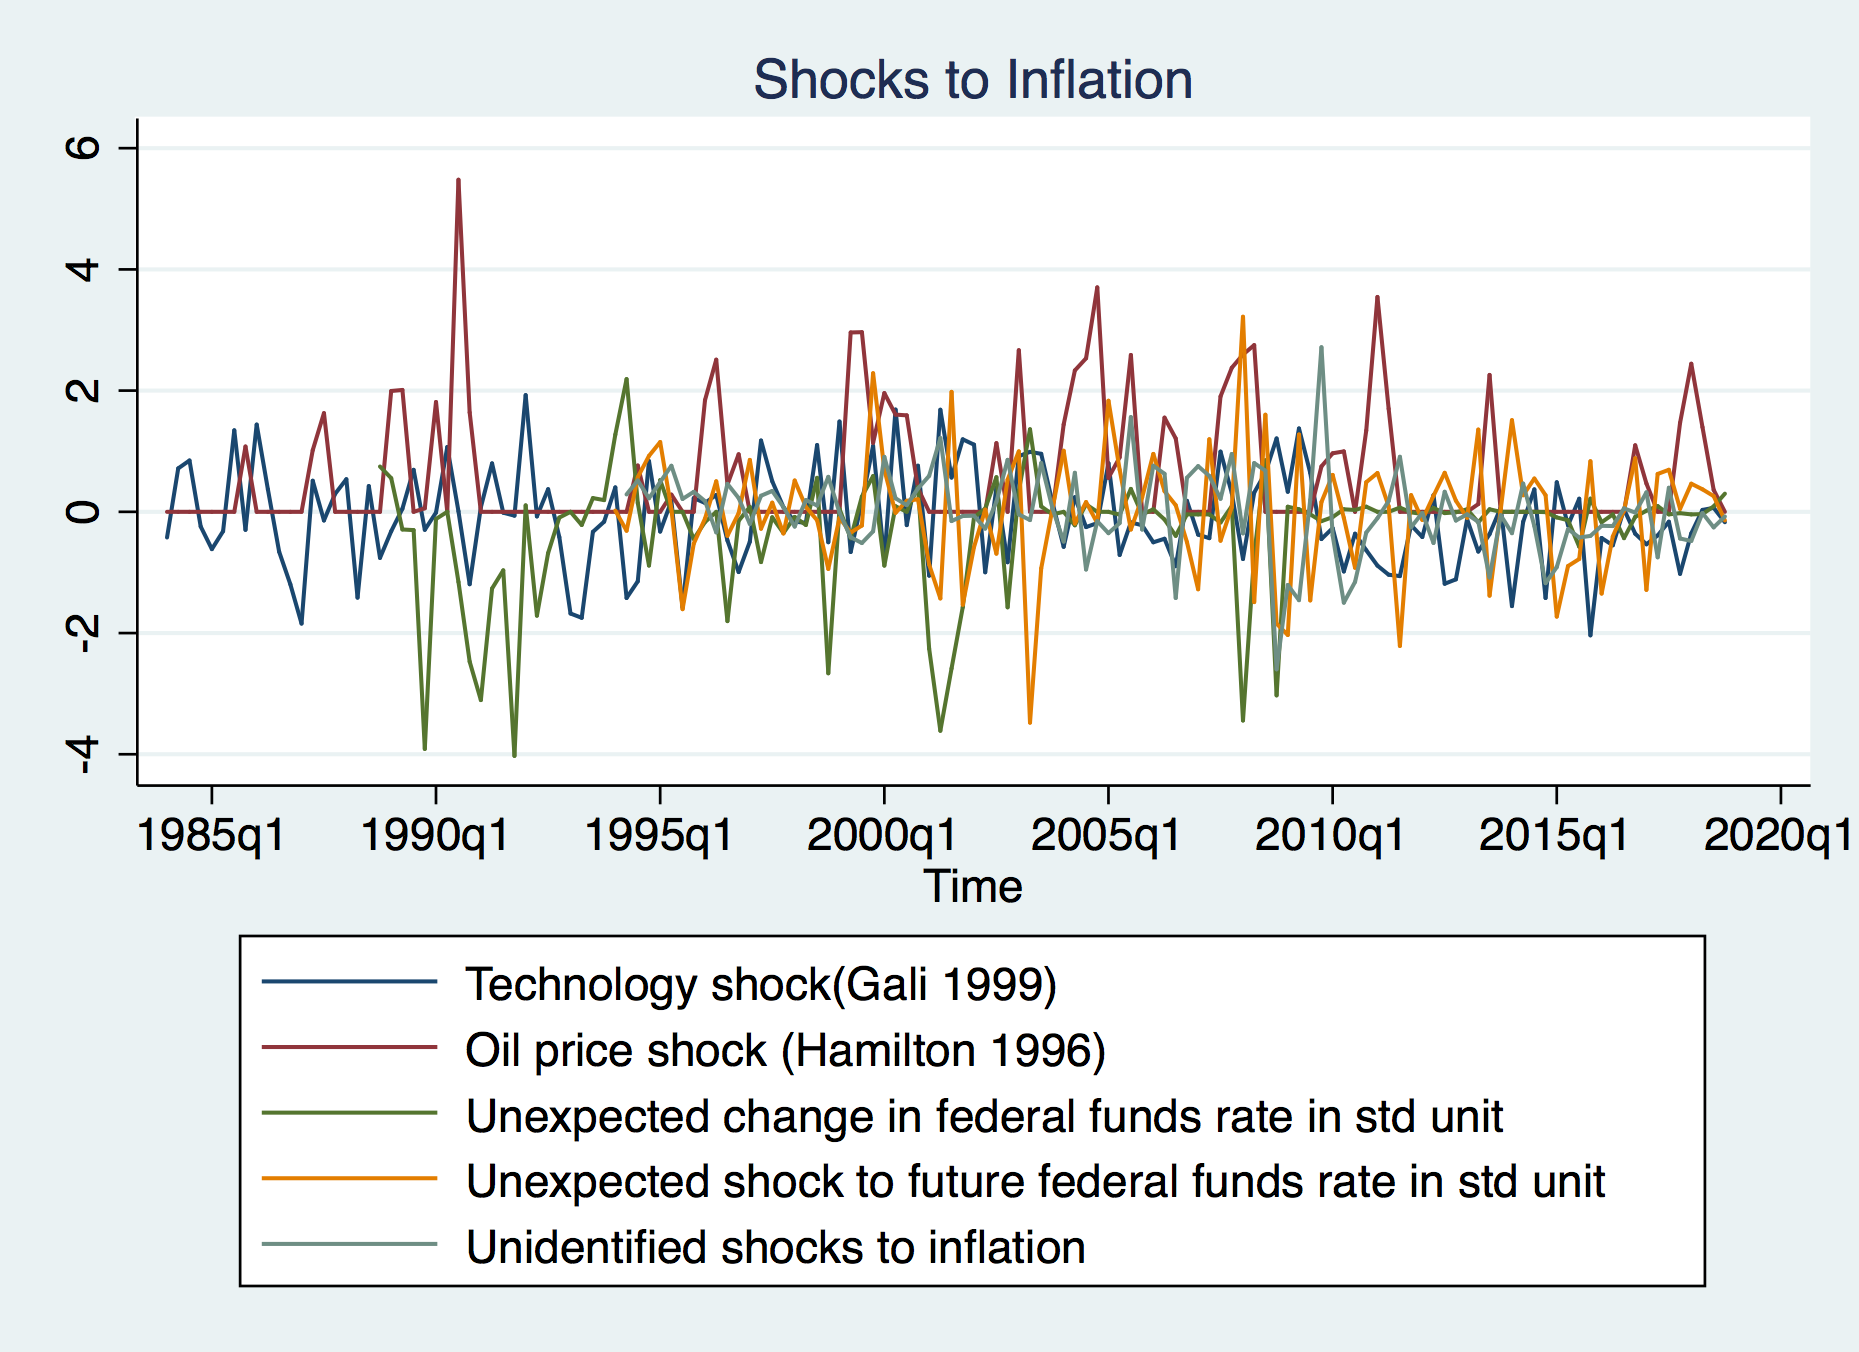
\includegraphics[width=0.7\textwidth]{figures/inf_shocksQ.png}
			\begin{flushleft}
			{\footnotesize Note: all the shocks are normalized by their sample standard deviation. Technology shock is idetified by long-run restriction of structural VAR with labor productivity, hours and inflation. Oil shock is defined as the max \{0, the largest increase of oil price over the past 12 months.\} }
		\end{flushleft}
		\caption{ Shocks to Inflation}
		\label{Inflationshocks}
	\end{figure}
	
	\subsection{Replicating \citet{coibion2012can}}
	
	For a direct comparison of my results and \citet{coibion2012can}, I first explore the impulse responses of CPI inflation $y_{t+k}$, SPF forecast errors and disagreement to one standard deviation of each shock at time $t$. In particular, the responses of disagreement is with respect to the absolute value of the shocks. Because CPI inflation forecast is available only after 1984, the sample period 1984-2007 is six years shorter than that in Figure 2 from \citet{coibion2012can}: 1976-2007. I do not include the results for PCE inflation as there is no PCE forecast during this period. 
	
	The underlying regression that produces impulse response estimates is  Equation \ref{IRRegression}, according to which inflation $y_t$ (or moments, $\overline {FE}_{t}$, $\overline{Disg}_t$ and $\bar \sigma^2_t$) in current quarter is a function of 4-period lags of itself and the realized shocks in current and previous period. The estimate of autoregression coefficients $\beta_\tau$ and shock-specific coefficients $\beta_{S,k}$ for different lags can be used to compute impulse responses of the variables of interest. In the impulse response graph, standard errors are computed using the parametric bootstrapping approach as in \citet{coibion2012can}. 
	
	\begin{eqnarray}\label{IRRegression}
		x_{t}  = \alpha + \sum^4_{\tau=1} \beta_{\tau} y_{t-\tau} +  \sum^1_{k=0} \sum_{S \in \{O,T\}}\beta_{S,k}\omega_{S,t-k} + \epsilon_t 
	\end{eqnarray}
	
	FIRE predicts $\beta_{S,k}=0\quad \forall k=1$ in the regressions with forecasts moments as dependent variable. i.e. forecasts react only to contemporaneous shocks instantaneously. Therefore, the average FE should not be dependent upon past shocks and  only experience a one-time rise and return zero immediately. The disagreements will not respond to the shock at all. 
	
	Left panel of the Figure \ref{ReplicateCoibionBefore2007} show results broadly consistent with \citet{coibion2012can} despite a wider confidence band possibly due to the change in inflation measures and the difference in the sample period. Productivity and oil price shocks are deflationary and inflationary, respectively. One standard deviation of productivity unsurprisingly brings down headline inflation by around 10 percentage points  in the first quarter and the negative impacts gradually mute since then till the 7-th quarter. Oil price shock of one standard deviation increases headline inflation by around 3 percentage points in the first quarter and the inflationary impacts last for 6 quarters. PCE inflation responds to both the shocks in a similar manner with slightly different magnitudes. The responses coefficients are statistically significant as the $95\%$ confidence interval stays on one side of zero for both shocks for the same period. 
	
	Second, population forecast errors respond to shocks in a sluggish manner as predicted in rigidity models. This is illustrated using both SPF's FE of CPI in the second graph of  left panel in Figure \ref{ReplicateCoibionBefore2007}. As we define the forecast error as point forecast minus realized value, forecast error rises(drops) after a positive(negative) shock and gradually return to zero around 4-5th quarters after the shock. 
	
	Lastly, SE and NI models imply disagreement pick up after shocks and gradually drop over the longer horizon.  Looking into the graph, the average response of disagreement to absolute value of  technology and oil shocks exhibit patterns similar to this prediction. Note now that the initial response is no longer statistically significant(same as the original result) and the pick-up of disagreement after both shocks do not take place immediately in the same quarter but in one quarter after the shock. \footnote{In addition, the degree of long-run disagreements sheds light upon one subtle difference between the SE and NI. Disagreements always exist in NI with the presence of private signals , in contrast, disagreement is zero over the long run in SE. }
	
	The responses to monetary policy shocks turn out to be noisier than those for technology and oil price shocks, as presented in the right panel of Figure \ref{ReplicateCoibionBefore2007}. On the top, I first plot the impulse response of inflation to path surprises $ED8ut$ and target surprise $MP1ut$, separately. On average, inflation reduces by around 10 percentage points after one unit increase of target surprise and increases by 10 percentage points following one unit of path surprise to federal funds rate. Both responses are  statistically significant in $10\%$  significance level. The unexpected future tightening causing a rise in inflation is consistent with the literature of the price puzzle. \footnote{See \cite{nakamura2018high} as an example of inflationary responses to a monetary tightening move of the Fed.}
	
	In the middle figure presents the responses of CPI forecast errors by SPF.  Although the average response seems to go in the same direction of the respective monetary shocks, consistent with the pattern seen for technology and oil price shocks, none of the responses are statistically significant and the estimates have big standard errors of 10-20 percentage points.  
	
	Similarly, the responses of disagreements to both monetary policy shocks in the bottom panel are not statistically significant throughout the 10 quarters.  
	
	How do we interpret the finding of non-response of forecasting error and disagreement to monetary policy shocks in the context of rigidity models? Non-response of FE suggests that on average professional forecasters have incorporated the monetary policy changes in their forecasts. Non-response of disagreements could be due to that forecasters ``agree'' on the realization of monetary policy shocks. Although the benchmark theory of SE and NI do not differentiate shocks, the evidence here seems to suggest that the degree of rigidity depends on the nature of the shocks. 
	
	Or there are other explanations.  First, overall the monetary policy shocks contribute only a small part of the variation in inflation compared to supply shocks. This was actually used by \cite{coibion2012can} to justify why monetary policy shock was not used in their exercise.  Second,  I am just running into the same difficulty in identifying real impacts of monetary policy shocks from low frequency data as all other papers addressing this issue. 
	

\begin{figure}[ht]
	\begin{subfigure}[b]{0.5\textwidth}
		\centering
		\caption{Technology and Oil Shocks}
		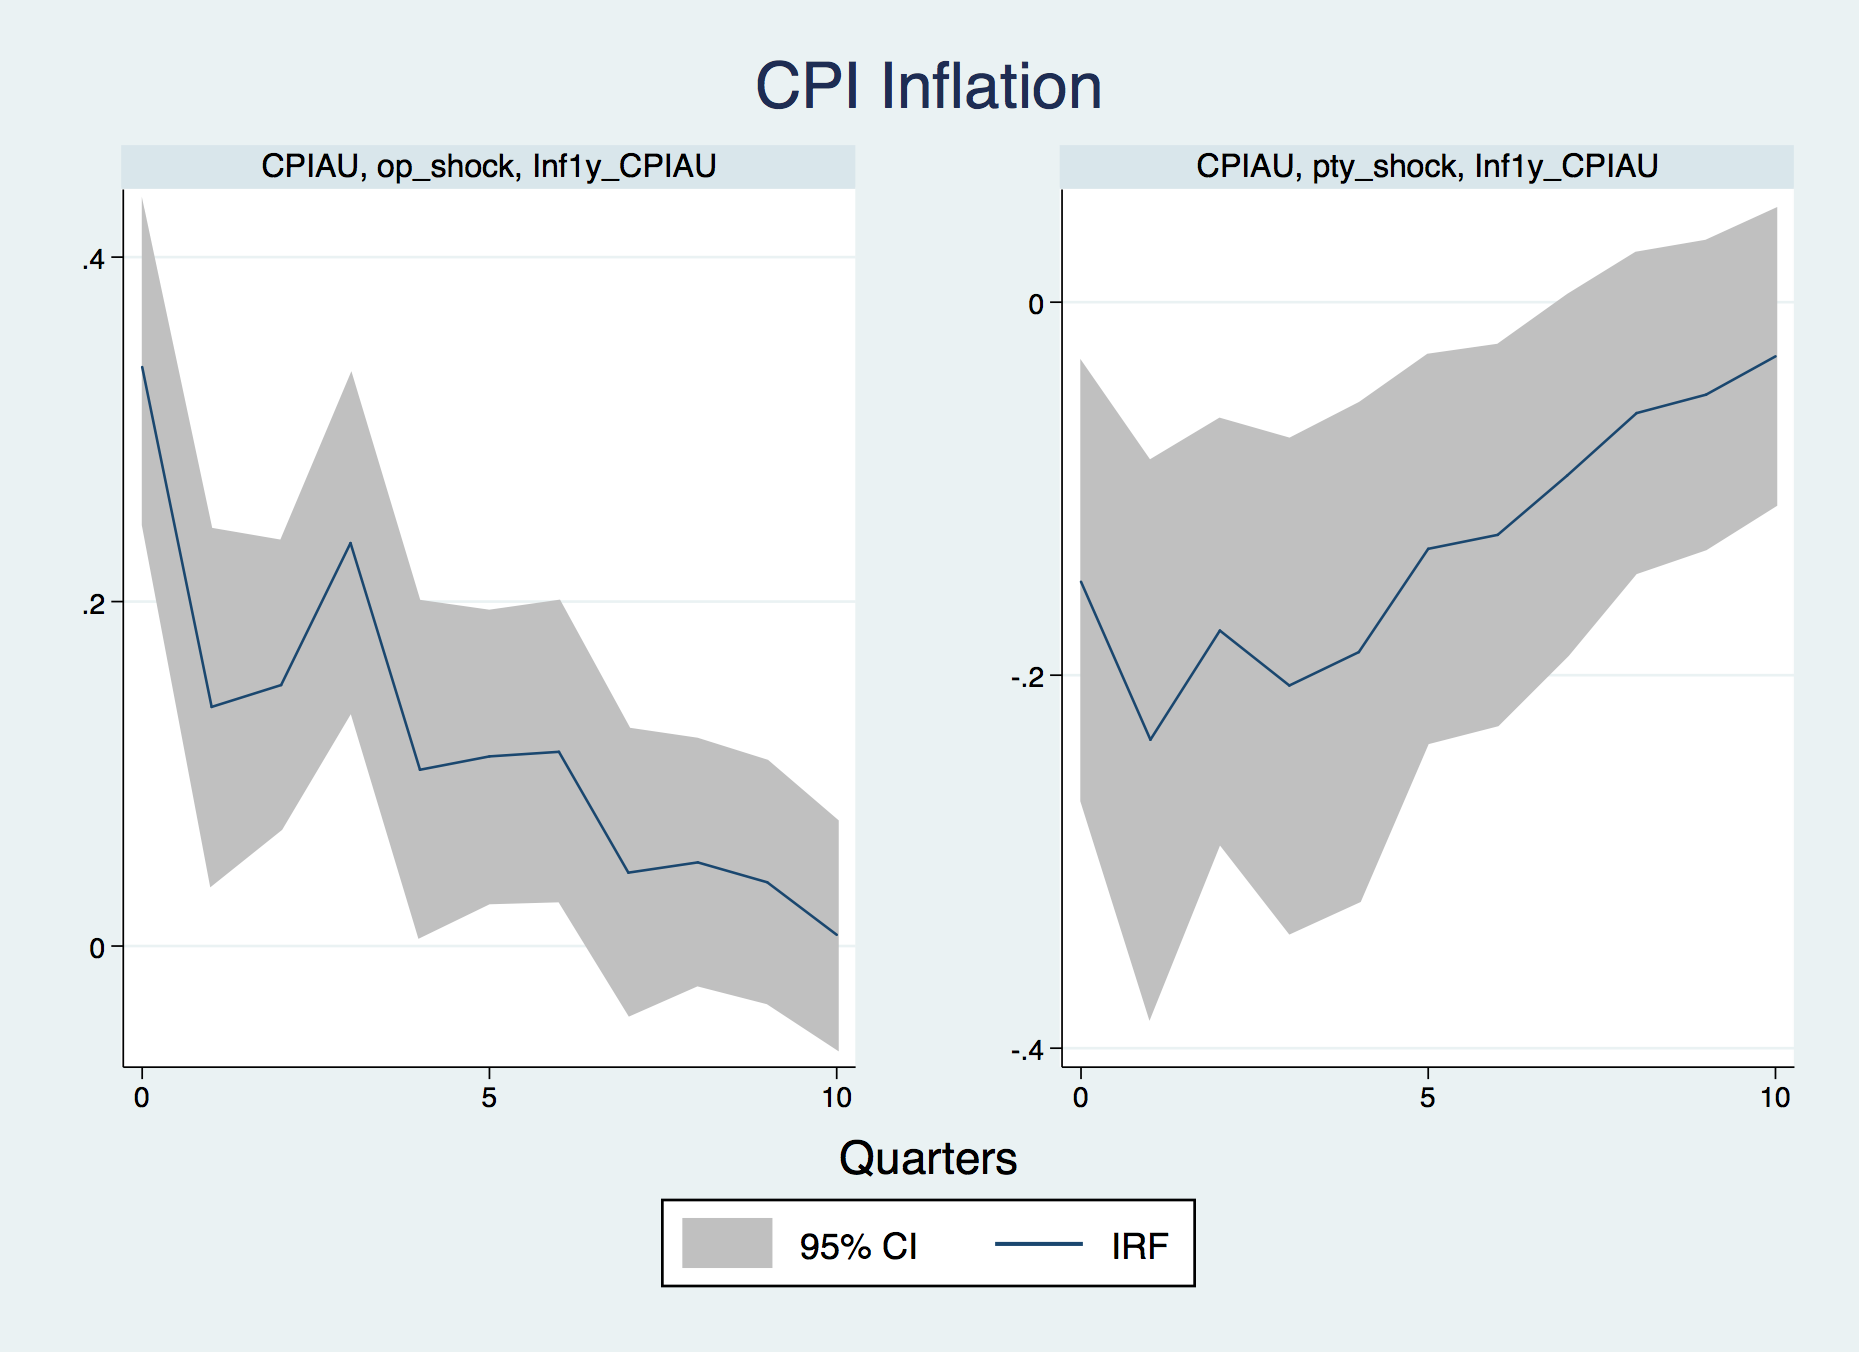
\includegraphics[width=7cm]{figures/CPIAU_ashocks_nmp_before2007.png}  
		\smallskip
		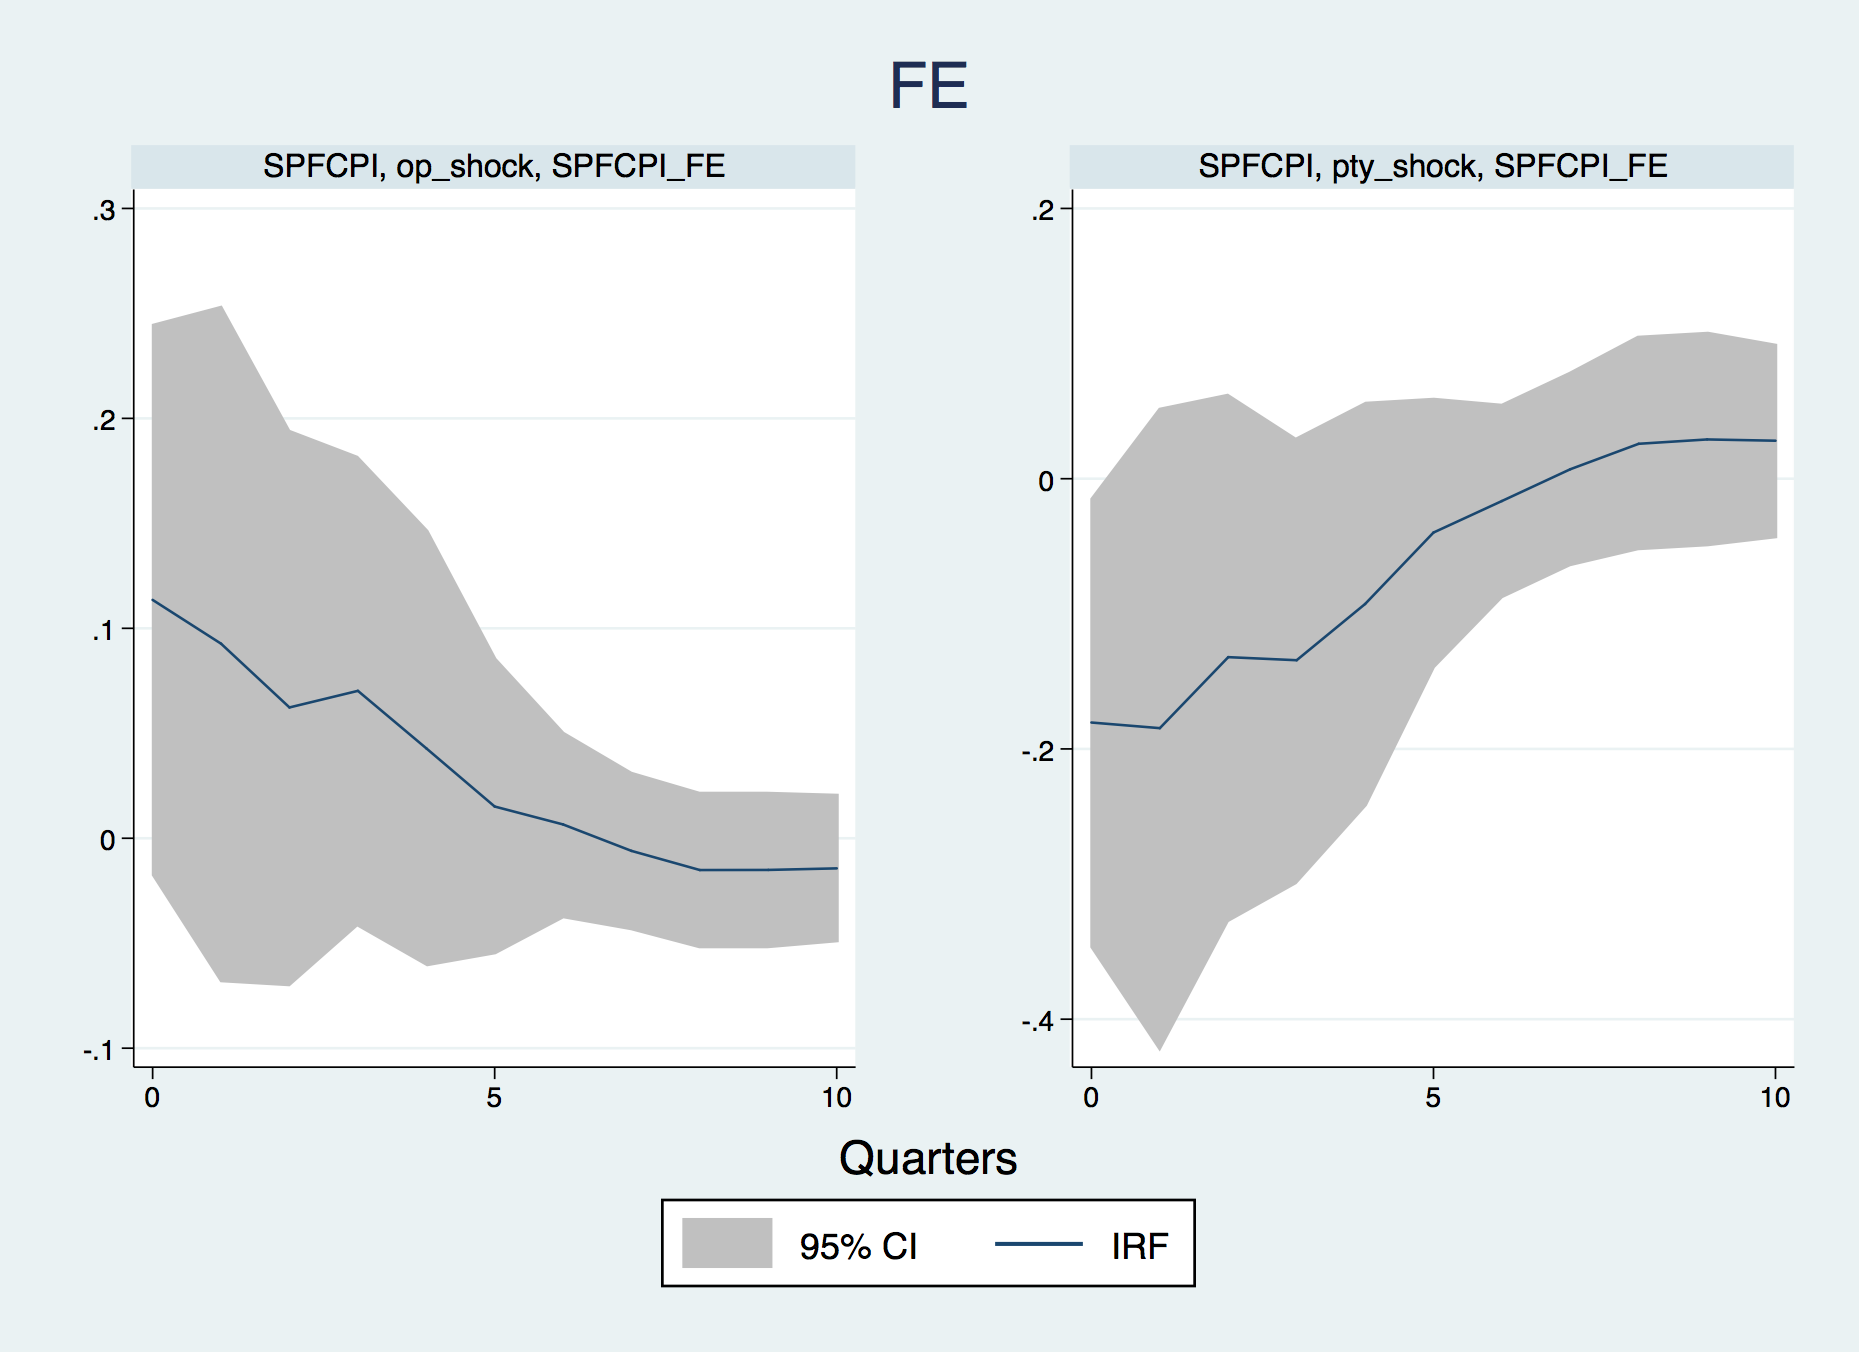
\includegraphics[width=7cm]{figures/SPFFE_ashocks_nmp_before2007.png} 
		\smallskip
		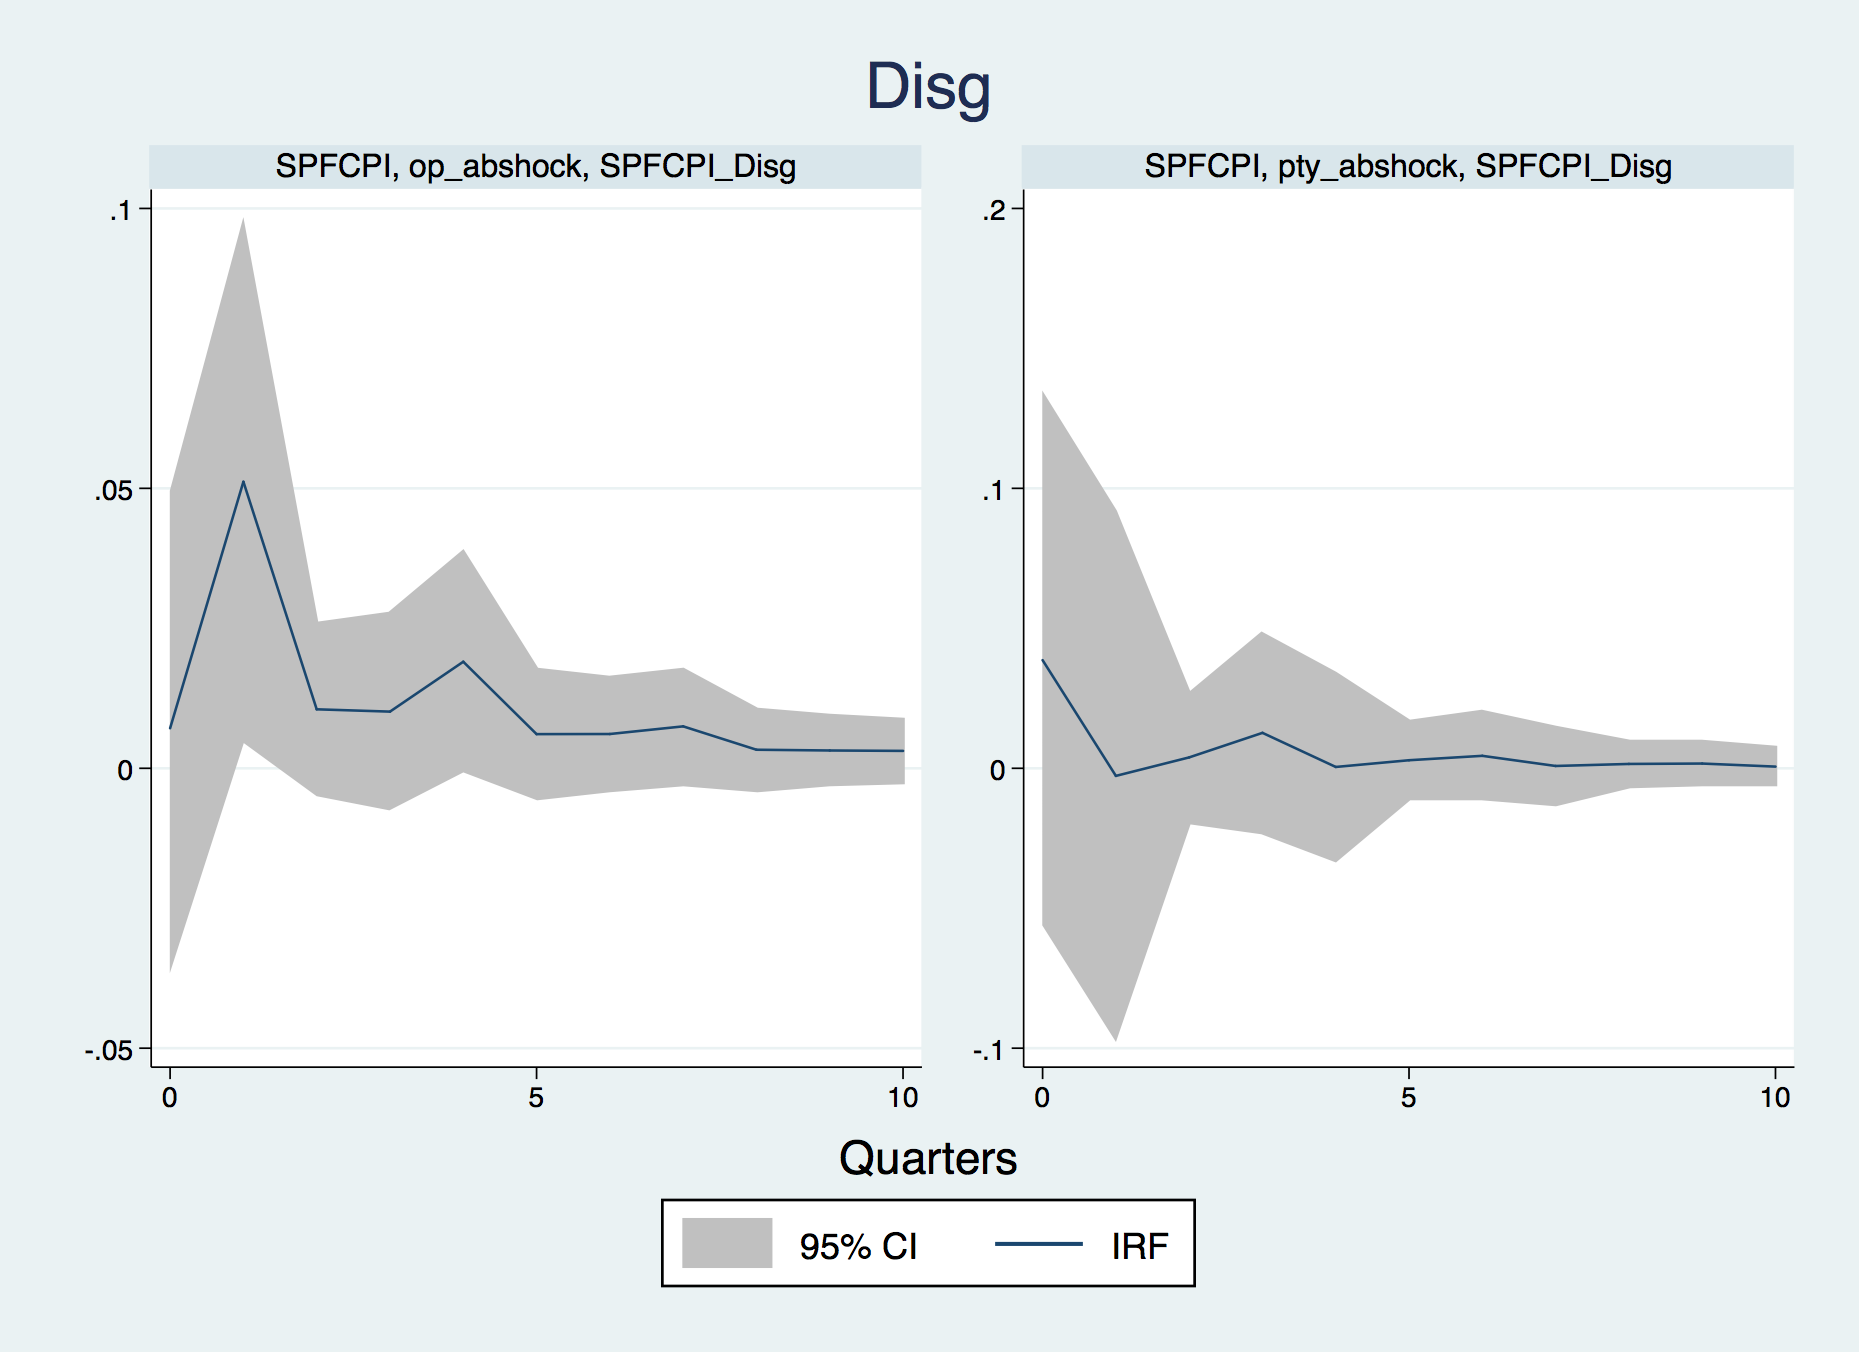
\includegraphics[width=7cm]{figures/SPFDisg_ab_ashocks_nmp_before2007.png} 
	\end{subfigure}
	\hspace{1em}
	\hfill
	\begin{subfigure}[b]{0.5\textwidth}
		\caption{Monetary Policy Shocks}
		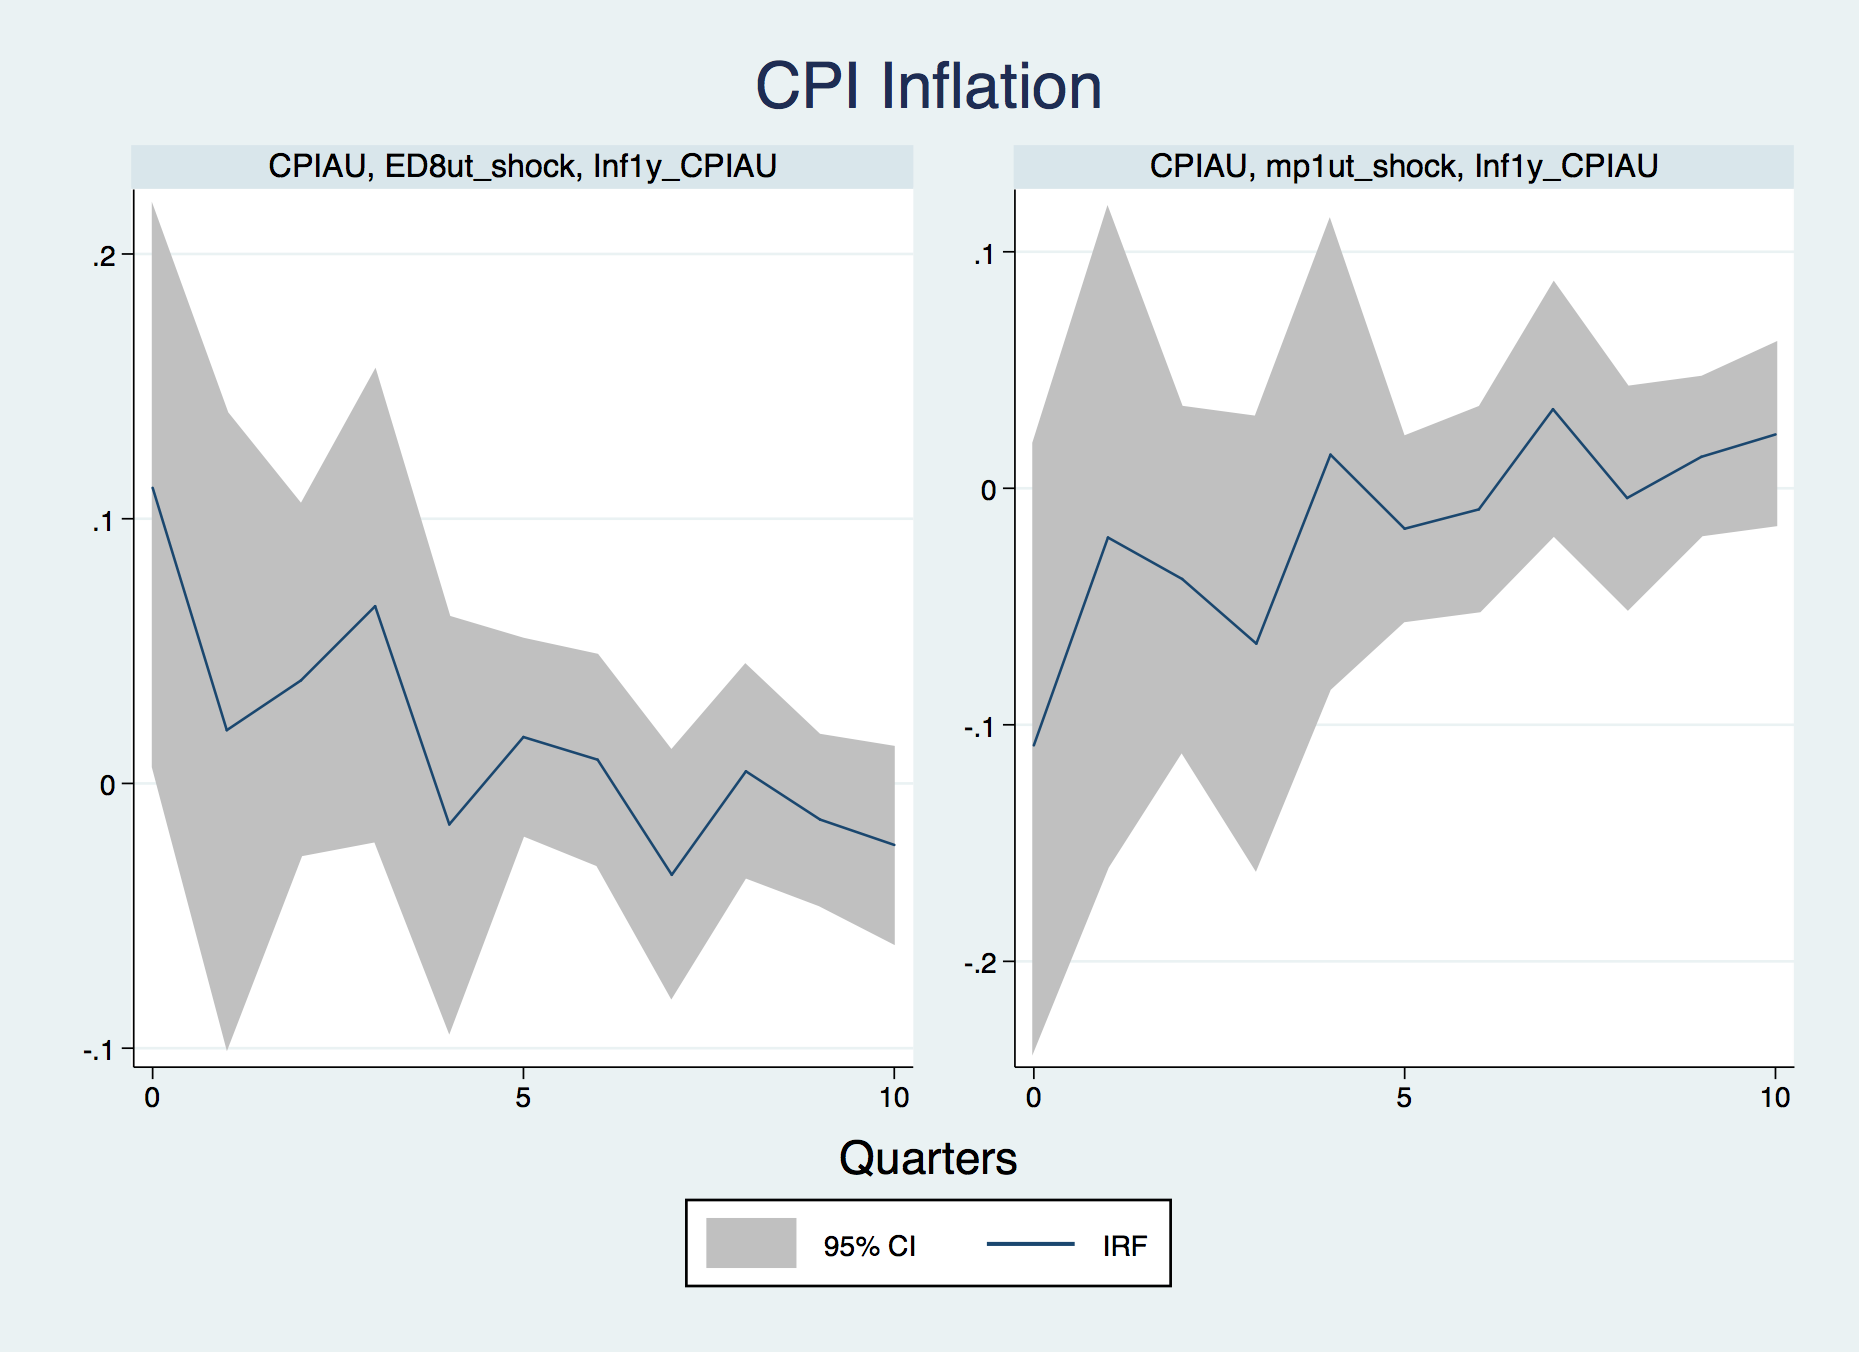
\includegraphics[width=7cm]{figures/CPIAU_ashocks_before2007.png} 
		\smallskip
		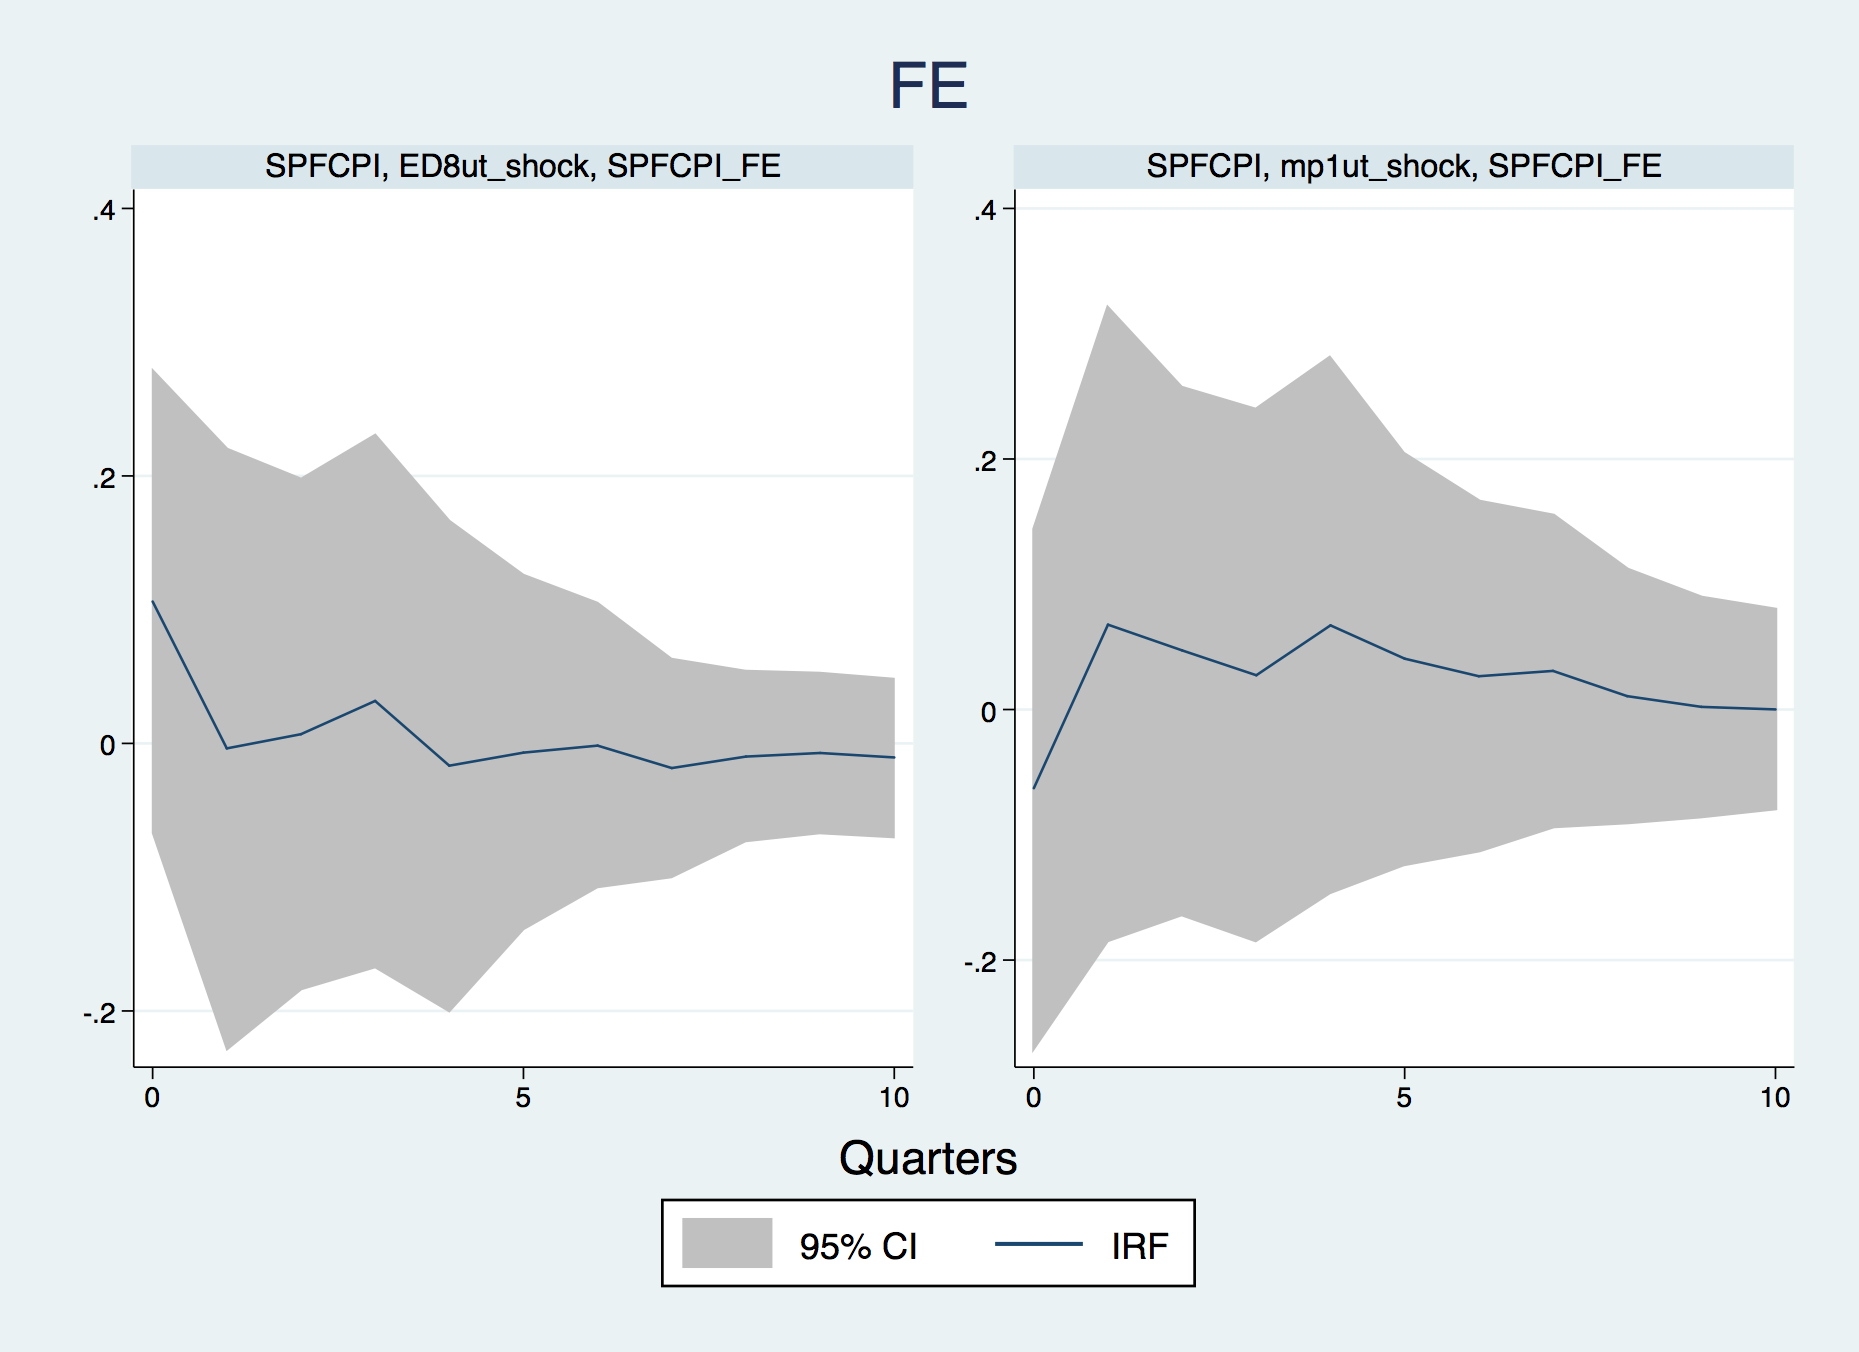
\includegraphics[width=7cm]{figures/SPFFE_ashocks_before2007.png} 
		\smallskip
		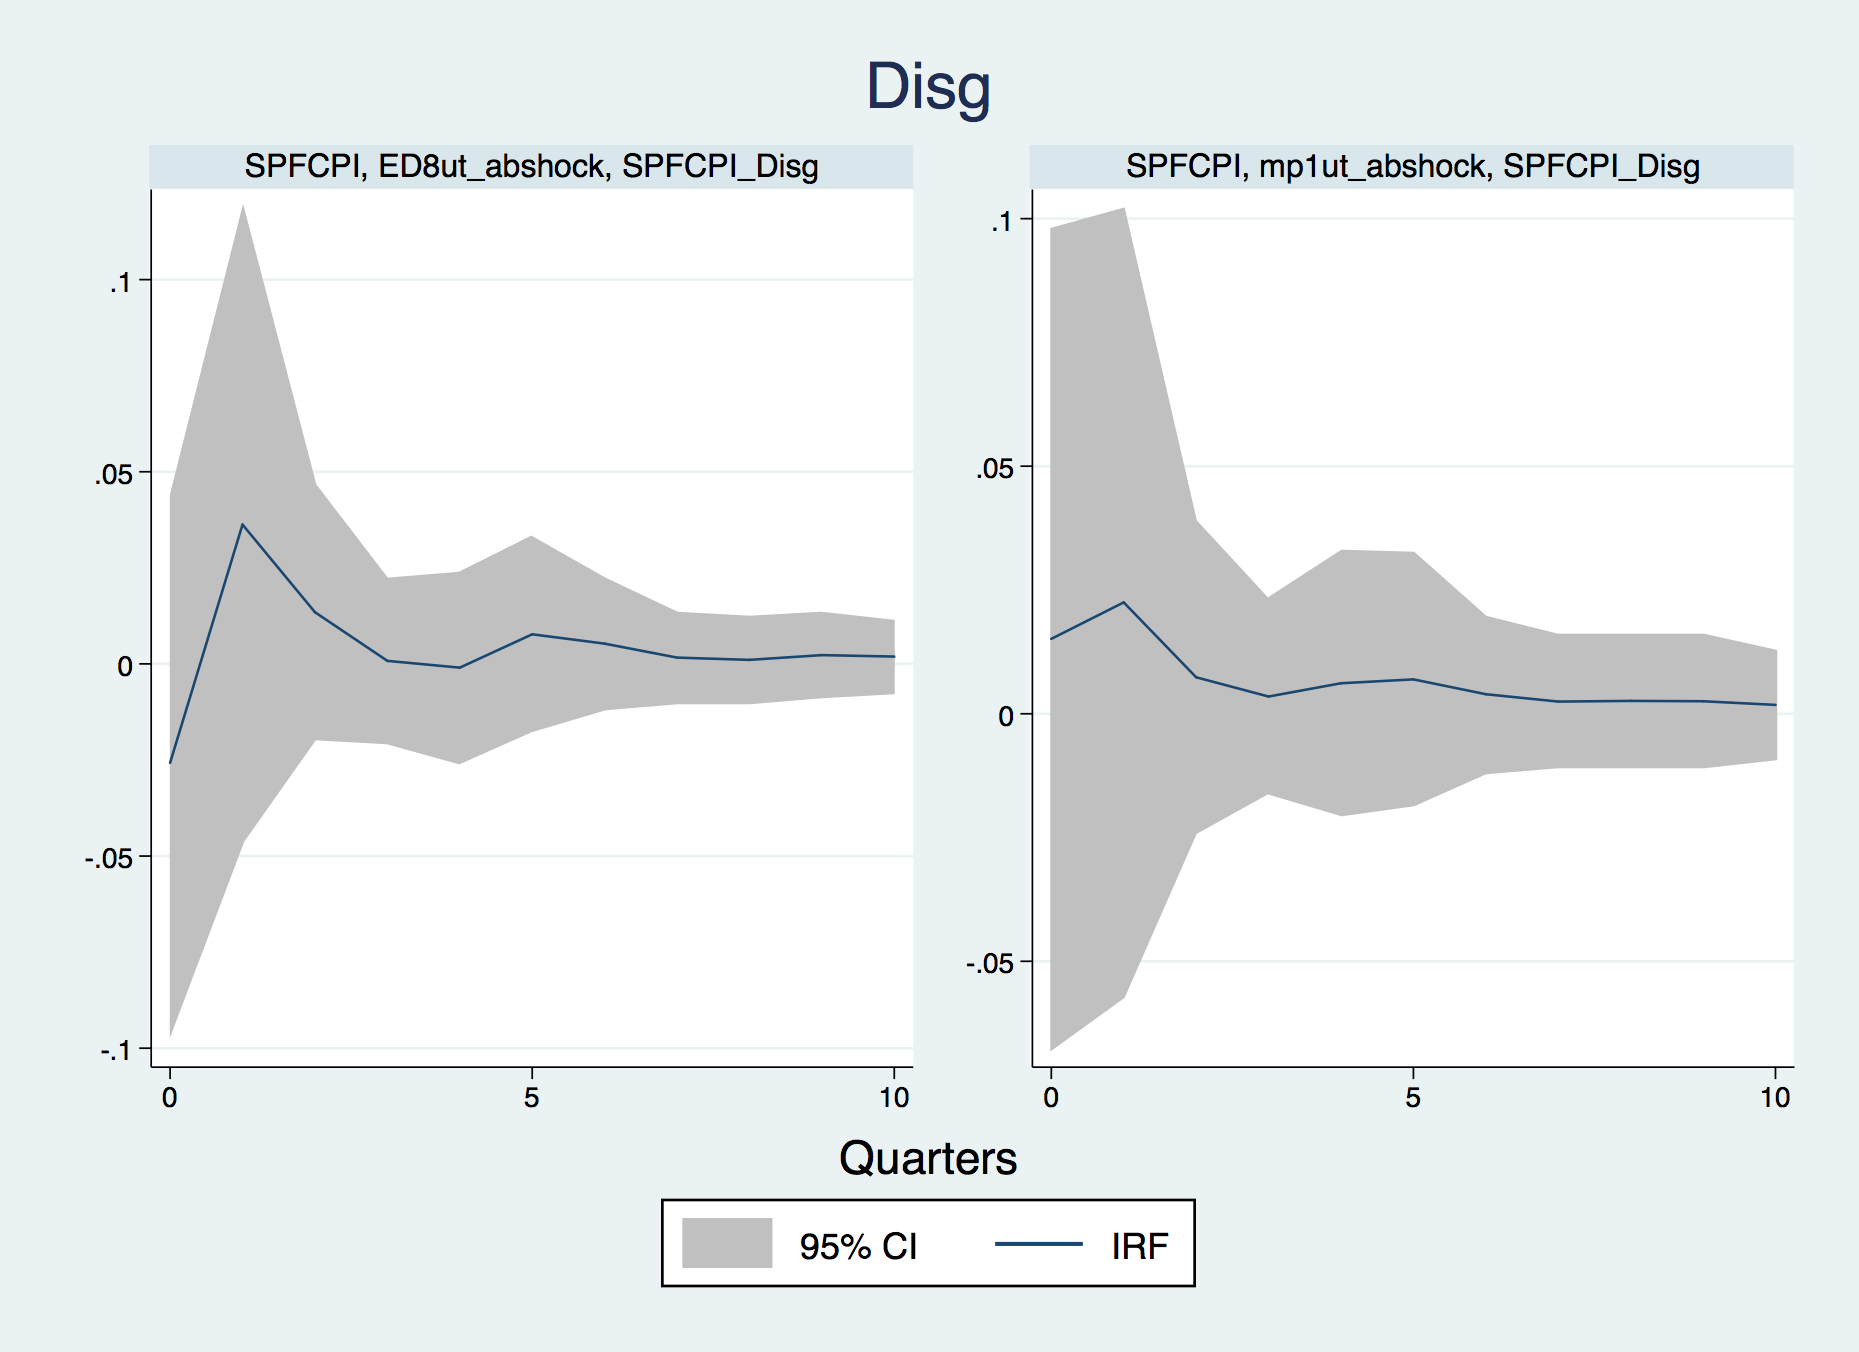
\includegraphics[width=7cm]{figures/SPFDisg_ab_ashocks_before2007.png} 
	\end{subfigure}
	\caption{Responses of Inflation and Professional Forecast Moments: 1984-2007}
	\label{ReplicateCoibionBefore2007}
\end{figure}

	
	\subsection{Additional evidence from uncertainty}
	
	In Figure \ref{ReplicateCoibionwholeperiod}, I extend the sample period to include the post-2007 years till 2019. Importantly, post2007 is the period when SPF starts surveying density forecasts that allow us to study the dynamics of uncertainty. In addition, the post crisis period has been characterized by a number of different features in terms of the behavior of macroeconomy(i.e. persistently low inflation) and monetary policy implementation (i.e. emphasis on monetary policy communication and zero lower bound), therefore it is worth examining if the patterns documented by \cite{coibion2012can} remain for the entire period. Also, since PCE inflation forecast is not available until 2007, I report results for both CPI and PCE as in previous analysis. 
	
	The left panel of  Figure \ref{ReplicateCoibionwholeperiod} presents impulse responses of average uncertainty of SPF in addition to that inflation, forecast error, disagreements in response to technology and oil price shocks. As shown in the top three figures, the results are consistent with that in Figure \ref{ReplicateCoibionBefore2007} for period before 2007.  Oil shock(technology shock) increases(decreases) inflation in the first quarter by 0.1 percentage  points, whose impacts last till 7-8th quarters. Confidence interval of the responses is smaller compared to previous figure probably due to larger sample size.  Average forecast errors react partially to the shock and gradually return to zero over the 4-5th quarters afterward. Disagreements picked up in the second quarter and return to zero 2 or 3 quarters  later. 
	
	
	The primary focus of this paper is the behavior of uncertainty. Its responses to the absolute value of various shocks are presented at the bottom of Figure \ref{ReplicateCoibionwholeperiod}. Since average uncertainty do not directly depend on the realizations and sizes of the shocks in various models, as shown in Equation \ref{VarREPop},  Equation \ref{VarSEPop}, and Equation \ref{VarNIEq}, the response of uncertainty cannot be used as a screening device of  FIRE from rigidity models. Instead, it checks the consistency of different theories with respect to the behavior of uncertainty.  
	
	The response graph seems consistent with this simple prediction, except for the uncertainty about CPI in responses to oil price shock. The responses of average uncertainty is not significantly different from zero throughout 10 quarters. \footnote{The impulse response that provides direct checking of rigidity models versus FIRE is the responses of revision in uncertainty, i.e. uncertainty about inflation in $t+h$ at time $t$ relative to $t-1$, $t-2$, etc. The results will be presented in a revised version of the paper.} 
	
	Impacts of monetary policies are shown in the right panel of Figure \ref{ReplicateCoibionwholeperiod}. Path surprise to federal funds rate, i.e. future monetary policy stances, again brings about the inflationary effect as before. One standard deviation of true tightening shock increases headline CPI inflation by around 0.15 percentage points in the first period.  In the same time, unexpected rate change does not affect inflation significantly once we include the post-2007 period.  One possible explanation for this is the small variation of target surprise after financial crisis, as illustrated in Figure \ref{Inflationshocks}. Except for the dramatic monetary loosening during financial crisis, there was little variation in the unexpected federal fund rate change.  
	
	Similar to results for pre-2007 period, the initial response of average forecast error to future tightening shock is statistically significant in the first period but insignificant soon after.  Interestingly, even though the target surprise does not affect inflation itself, forecast errors do react to it in an inflationary manner. The magnitude of the response is as large as 0.25 percentage points in the first quarter. Rigidity models predict forecast errors depend on past shocks, while there does not seem to be strong evidence for this when it comes to monetary policy shocks. Forecasters reaction to monetary policy shocks appear to more efficient than for supply shocks. 
	
	Disagreements show little response to monetary policy shocks as well, with the only exception being PCE forecast with respect to path surprise. The estimates of these responses are not  significantly from zero throughout the entire horizon. Non-response of disagreements could arise if forecasters have incorporated the monetary policy shocks (thus the shock no longer qualified as a ``shock'') , or all forecasters simultaneously incorporating the realization of the monetary shocks. In the context of NI model, the disagreements can only arise with the presence of private signals. Therefore, monetary policy being a more public signal can help explain the muted response of disagreements in comparison with other shocks. \footnote{Another explanation is that monetary policy actually coordinates agents' expectations, thus accordingly reduce disagreements, according to \citet{morris2002social}. This mechanism can mute the response of disagreements.}
	
	Lastly, average uncertainty do not react to monetary policy shocks in the extended period. None of the response is significantly different from zero. This is the same with technology and oil price shocks. 
	

		\begin{figure}[ht]
		\begin{subfigure}[b]{0.5\textwidth}
			\centering
			\caption{Technology and Oil Shocks}
			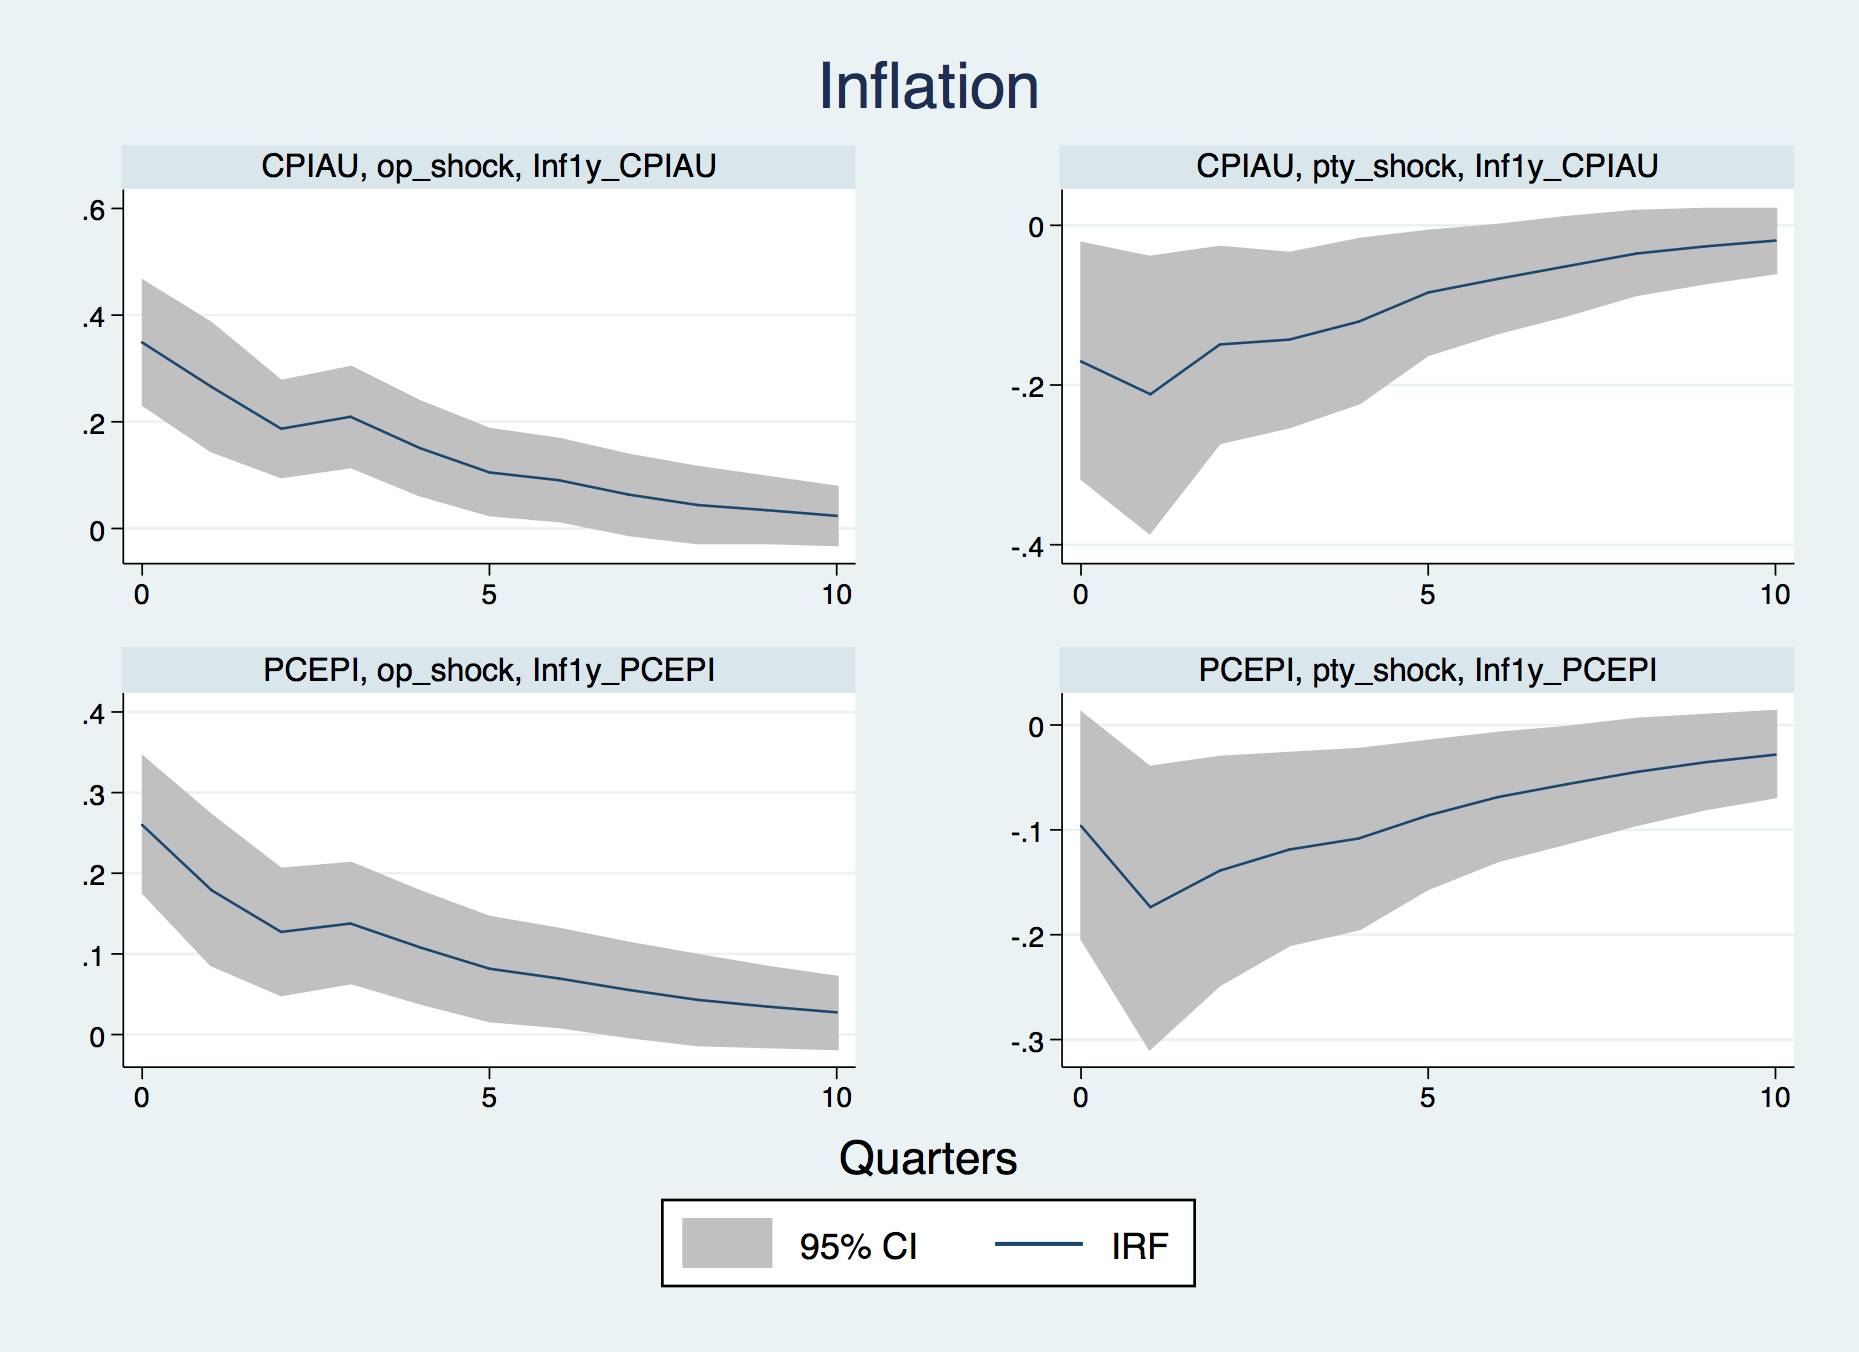
\includegraphics[width=7cm]{figures/Inf_ashocks_nmp.png}  
			\smallskip
			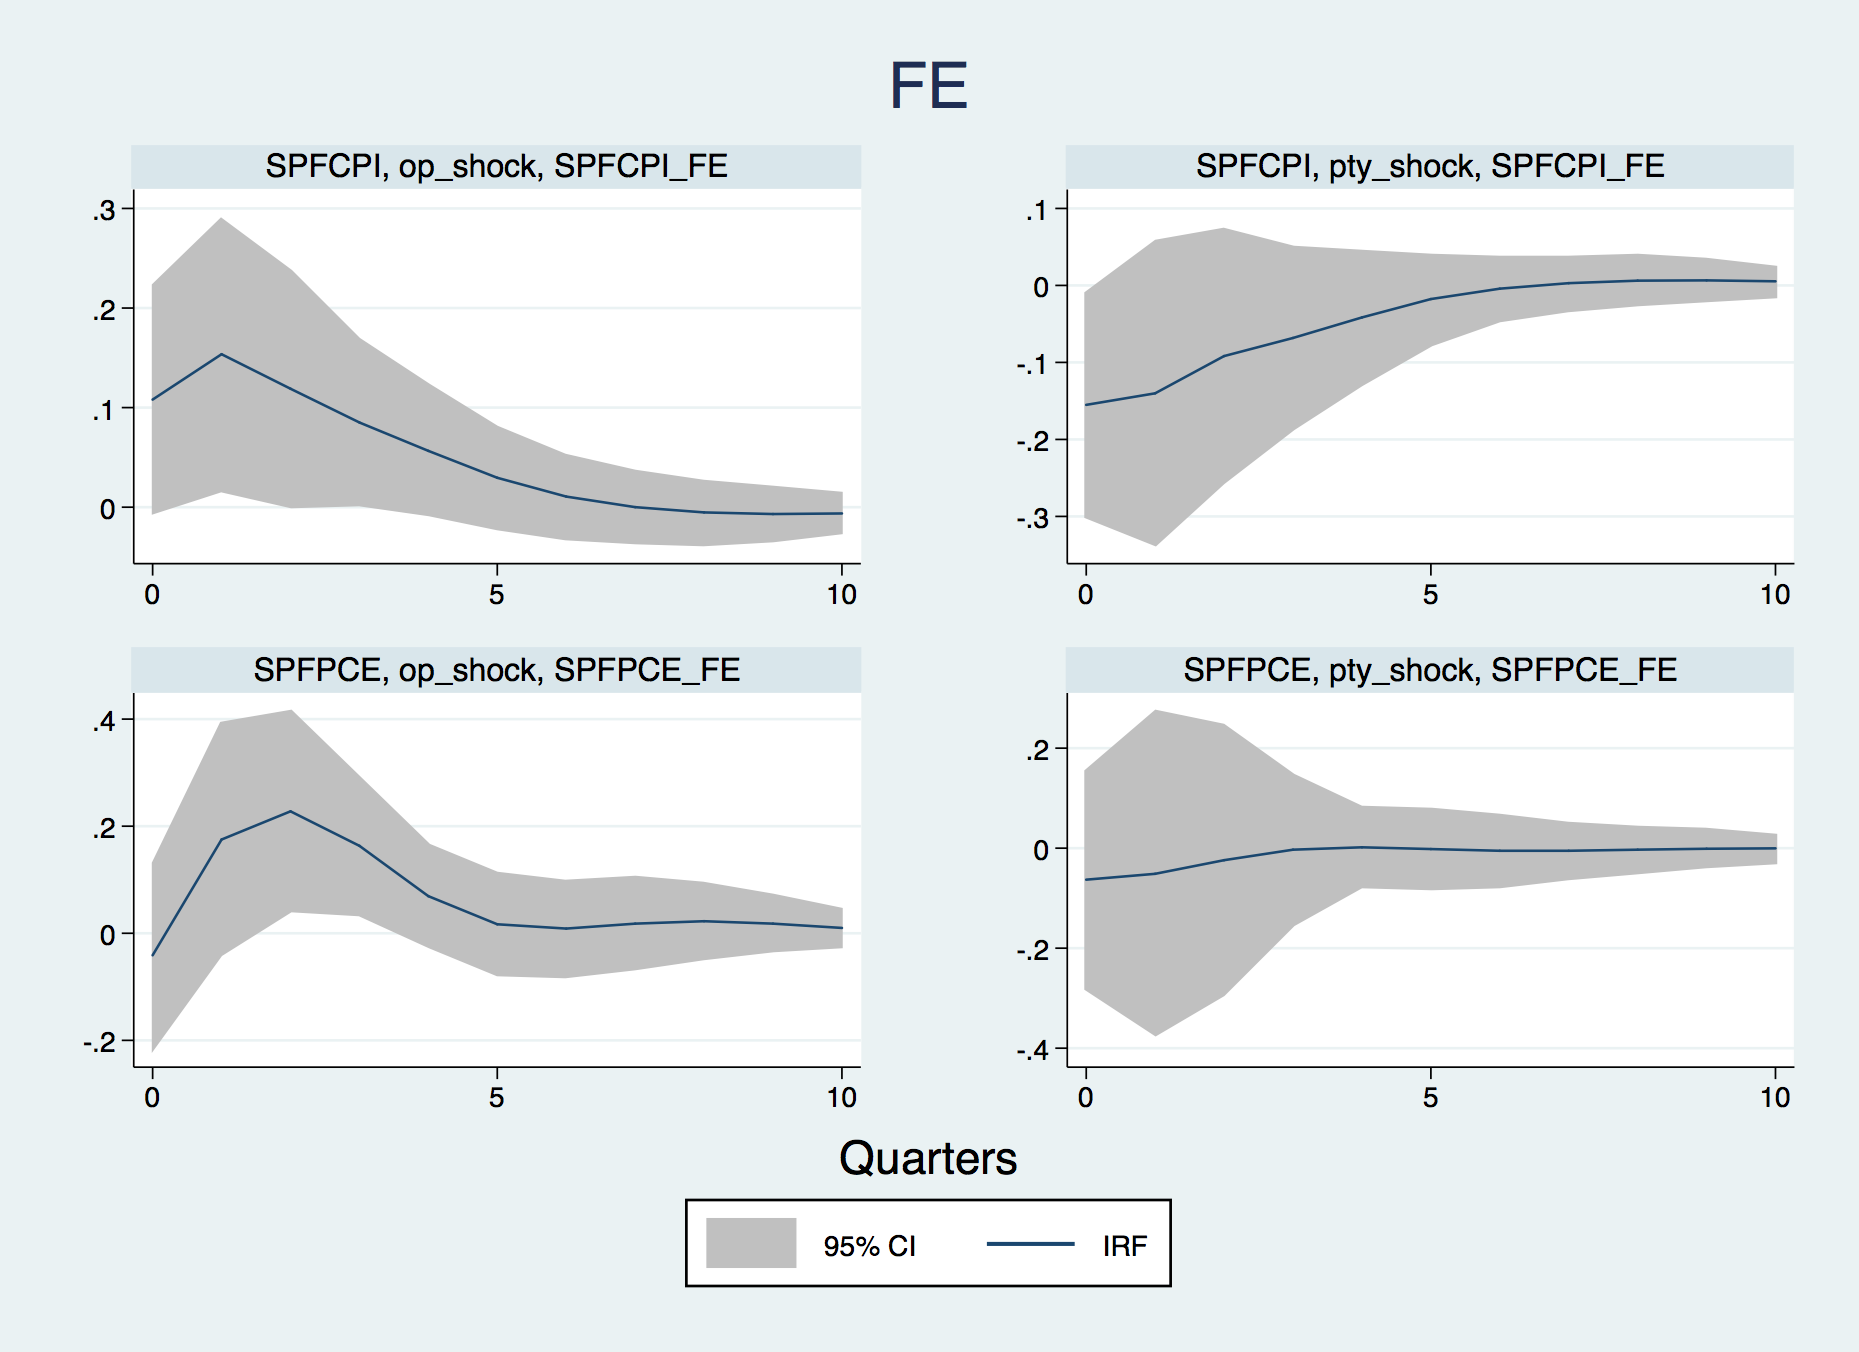
\includegraphics[width=7cm]{figures/SPFFE_ashocks_nmp.png} 
			\smallskip 
			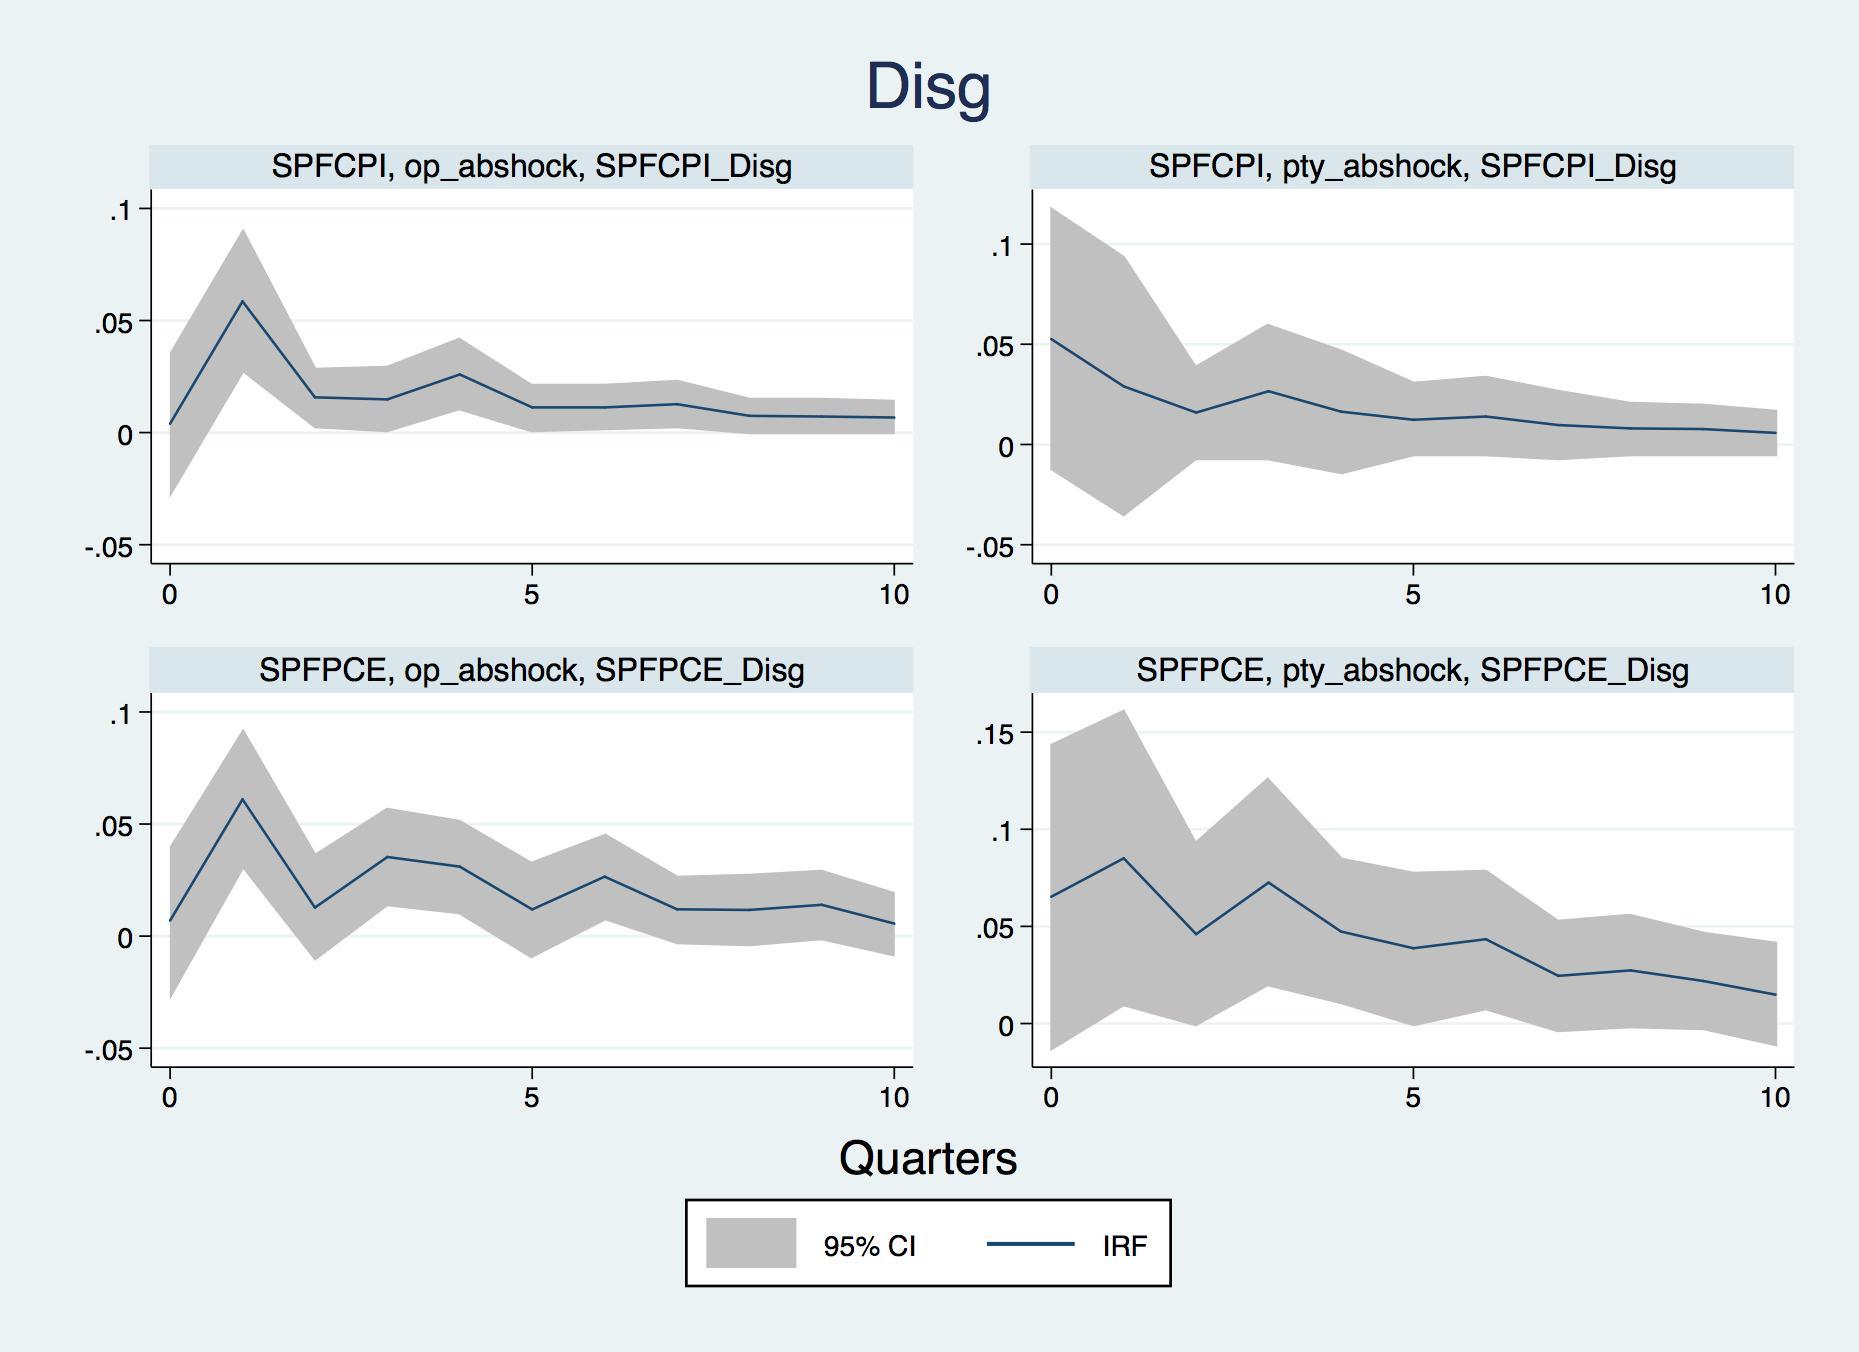
\includegraphics[width=7cm]{figures/SPFDisg_ab_ashocks_nmp.png} 
			\smallskip 
			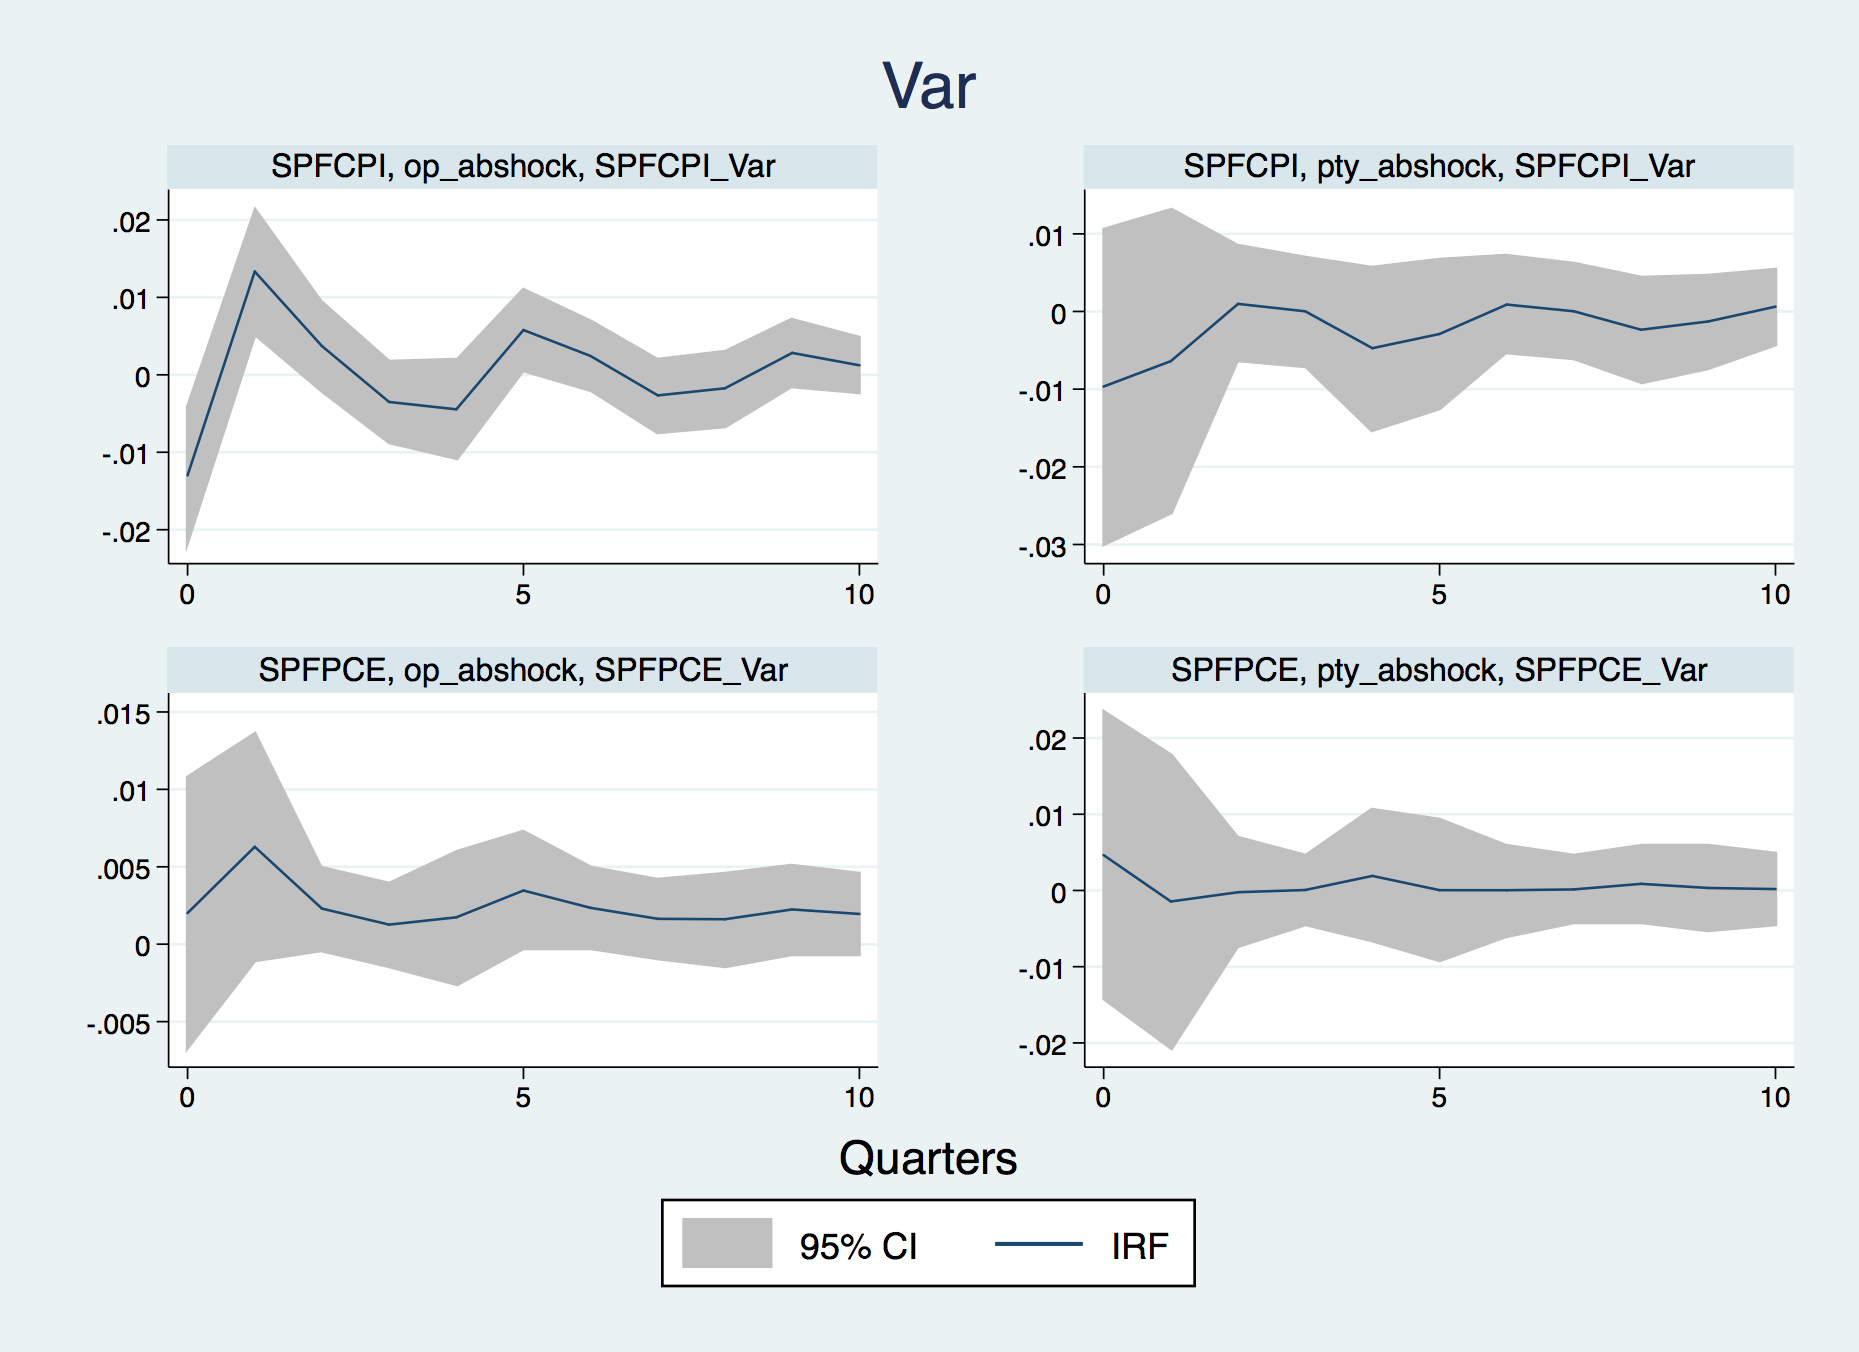
\includegraphics[width=7cm]{figures/SPFVar_ab_ashocks_nmp.png} 
		\end{subfigure}
		\hfill
		\hspace{1em}
		\begin{subfigure}[b]{0.5\textwidth}
			\caption{Monetary Policy Shocks}
			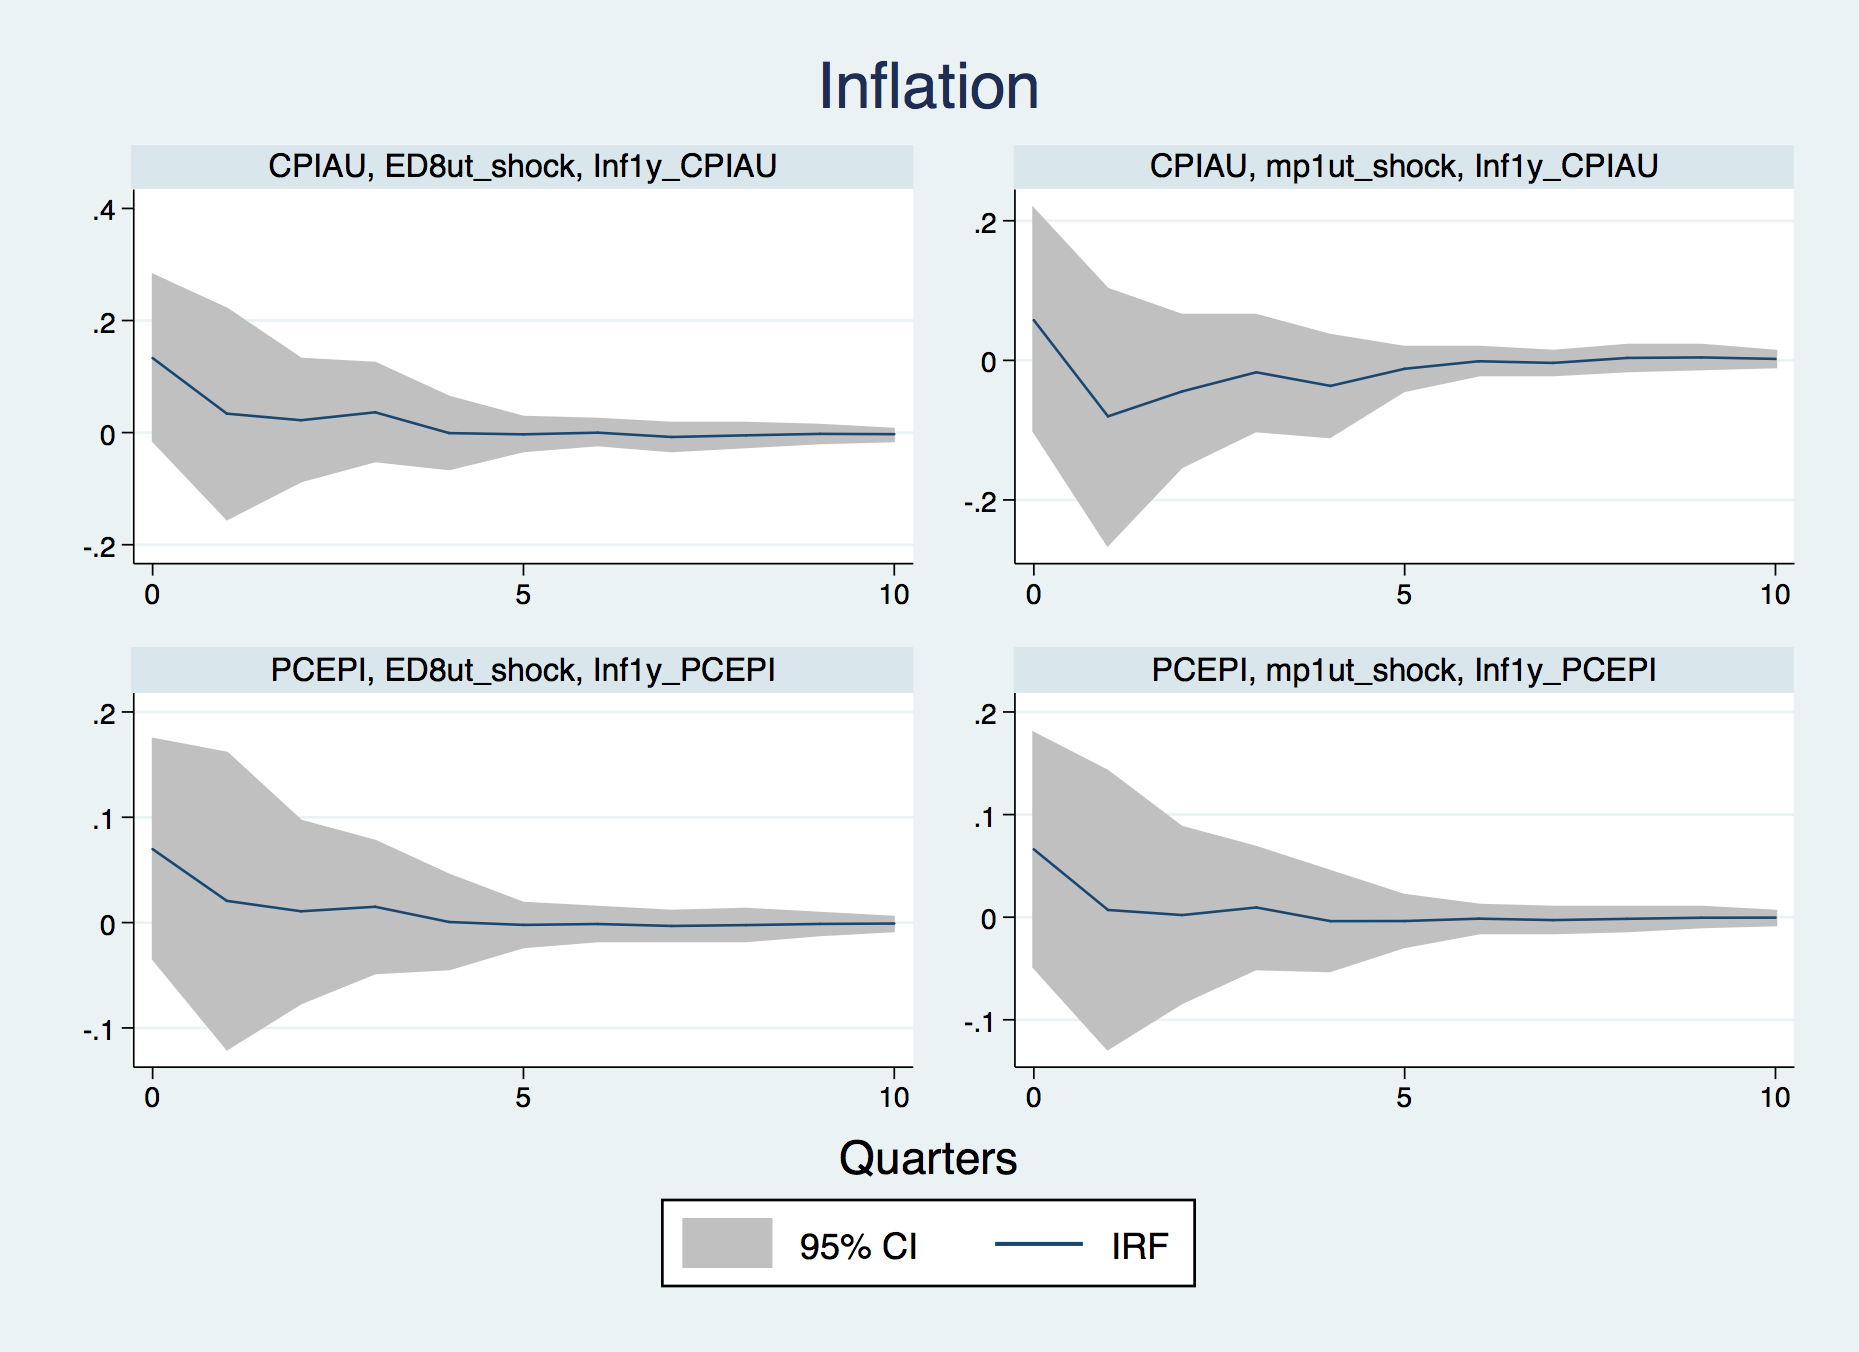
\includegraphics[width=7cm]{figures/Inf_ashocks.png} 
			\smallskip
			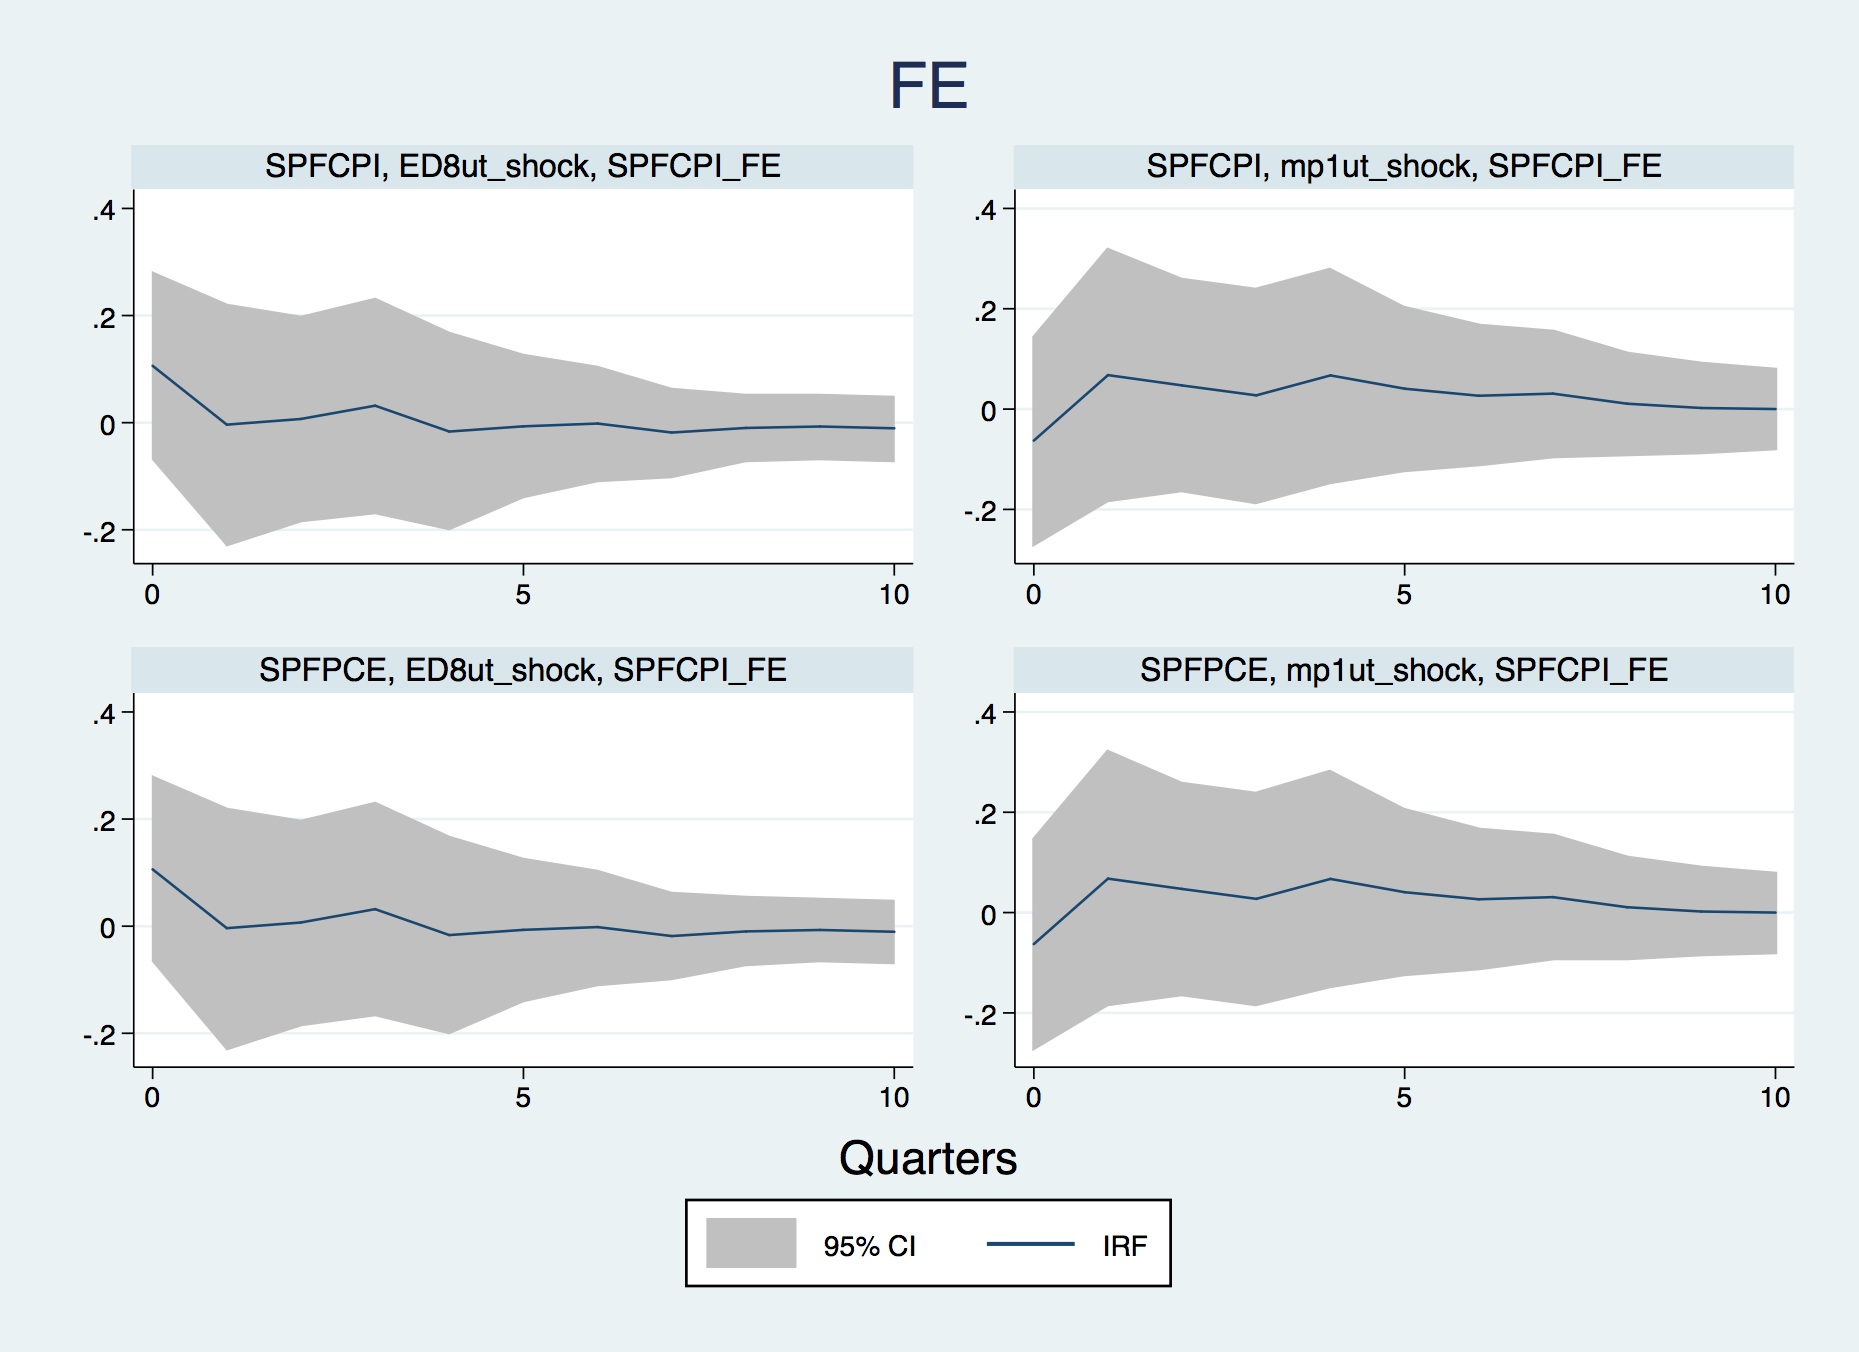
\includegraphics[width=7cm]{figures/SPFFE_ashocks.png} 
			\smallskip
			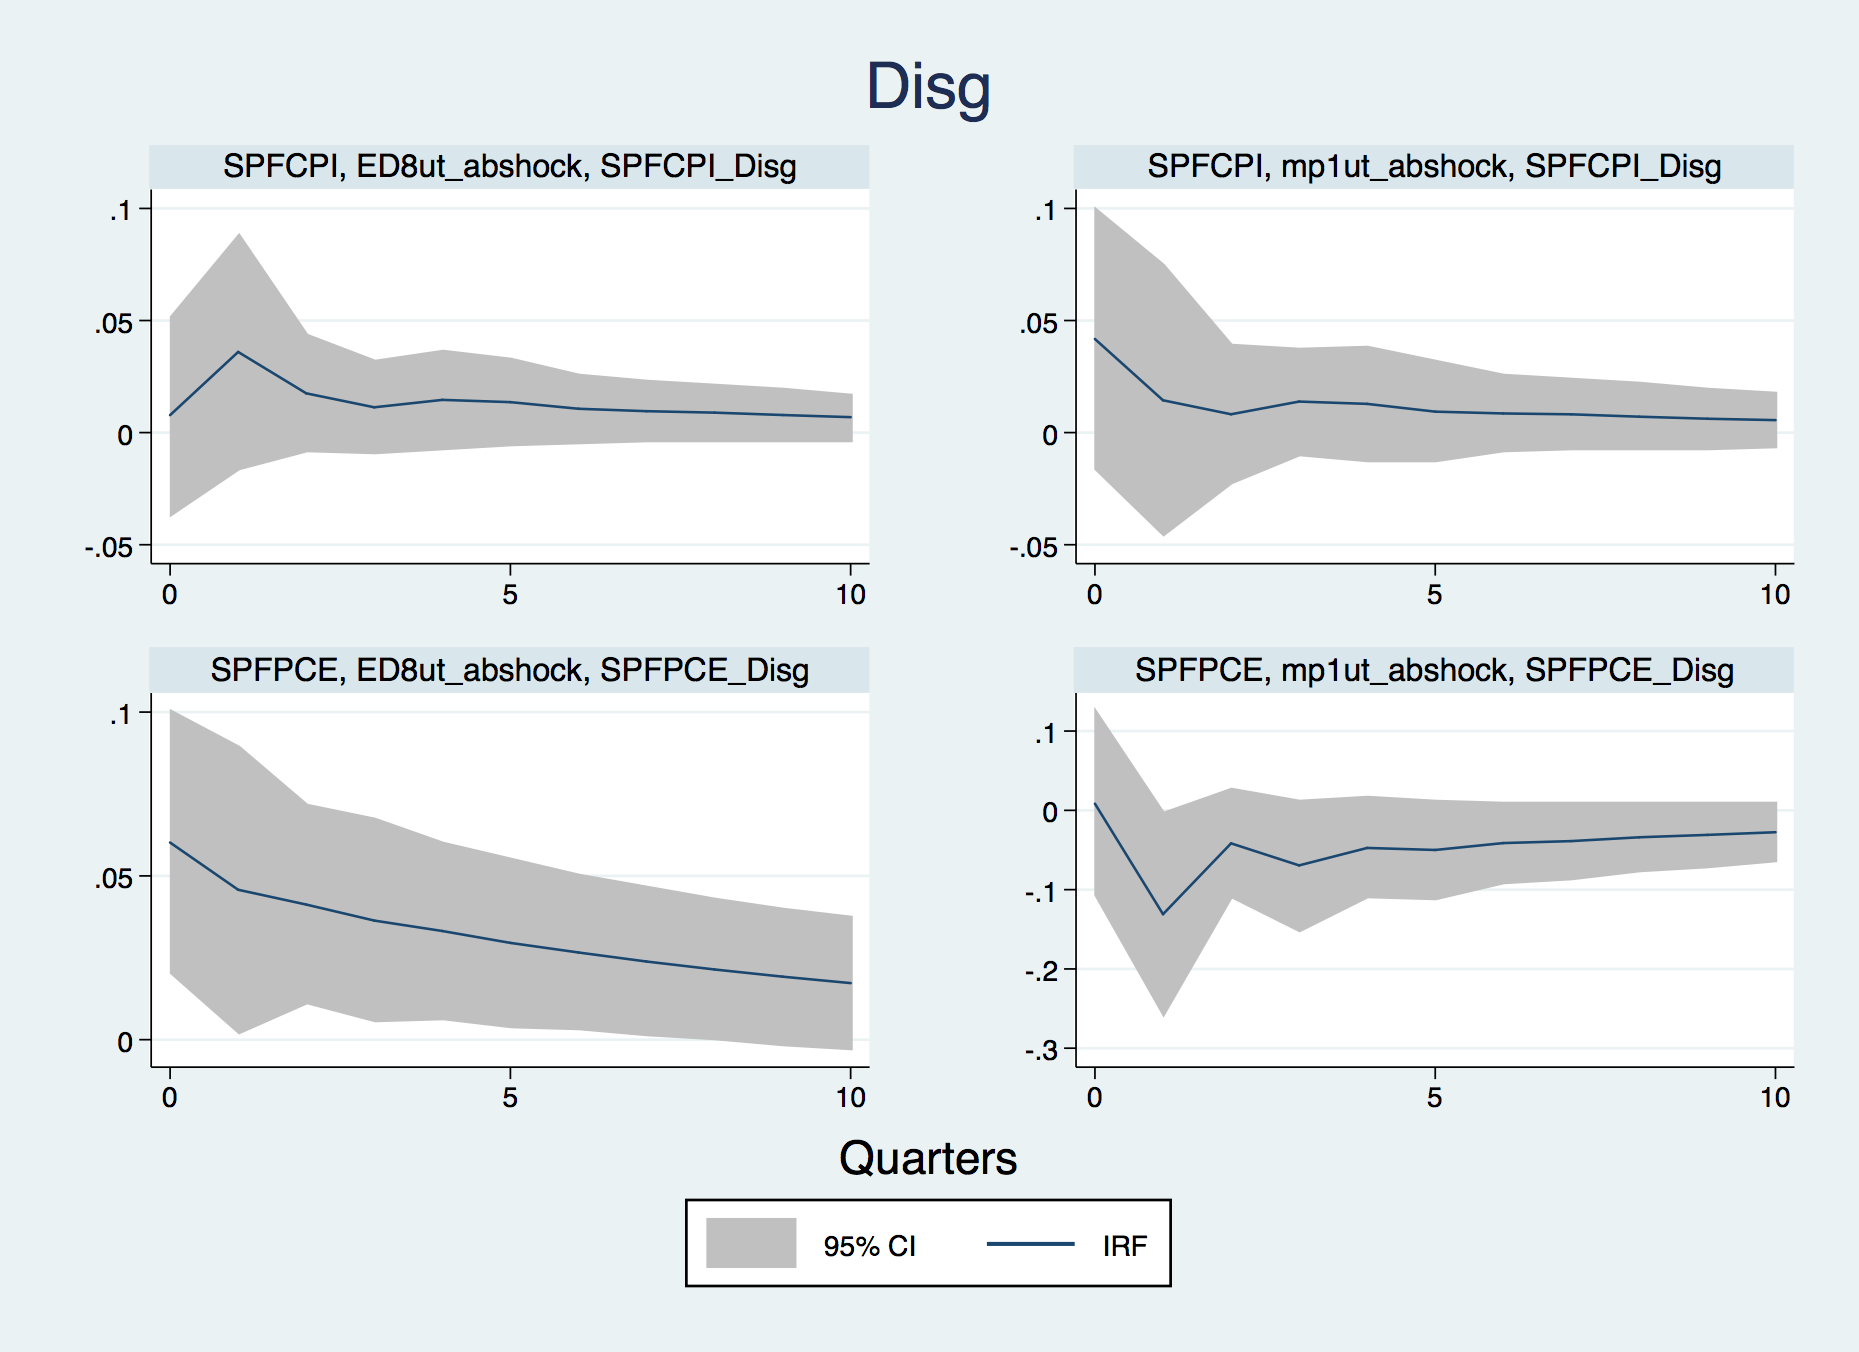
\includegraphics[width=7cm]{figures/SPFDisg_ab_ashocks.png} 
			\smallskip
			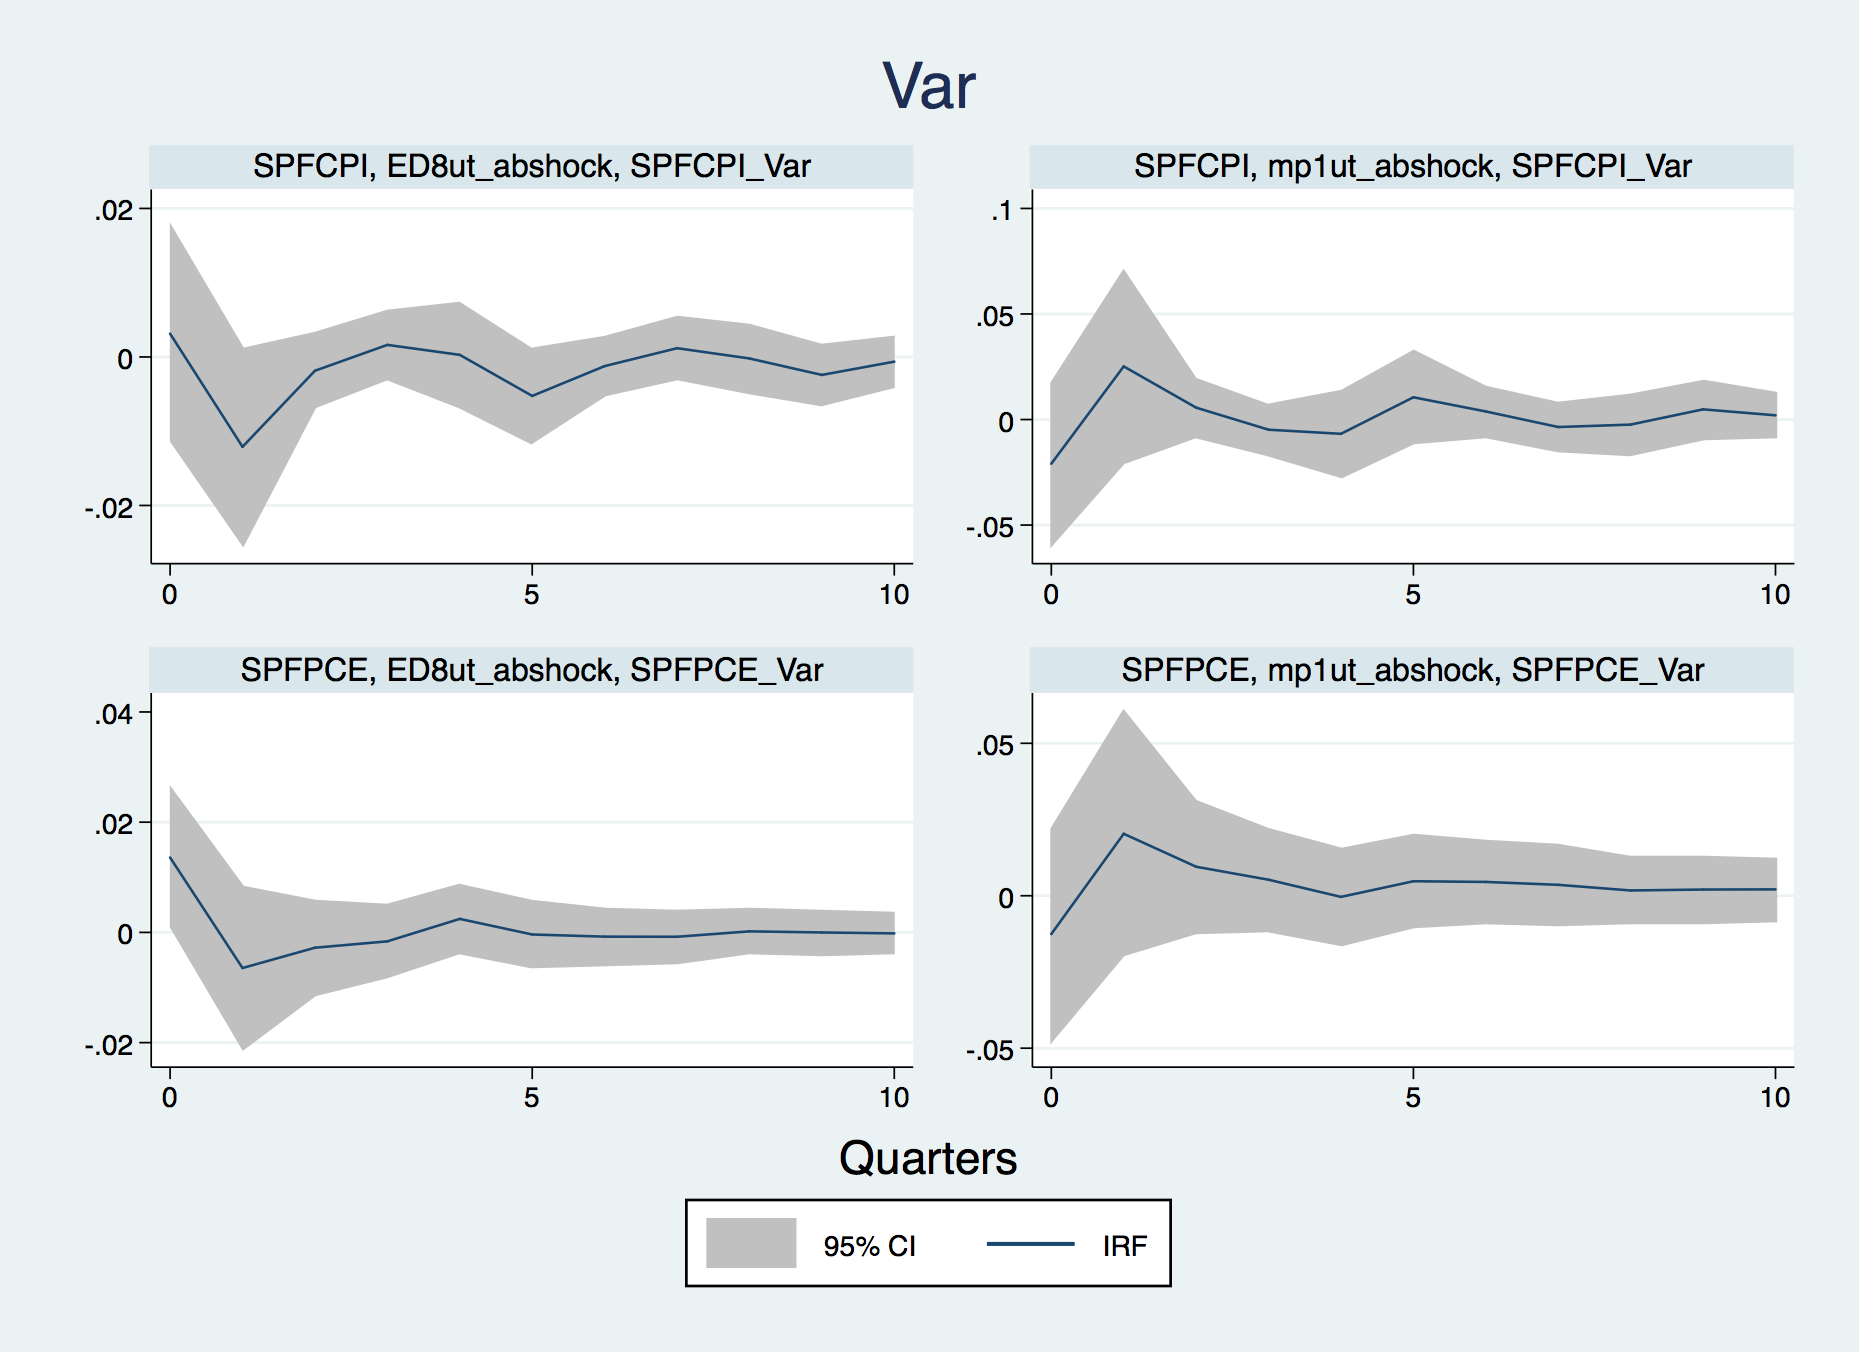
\includegraphics[width=7cm]{figures/SPFVar_ab_ashocks.png} 
		\end{subfigure} 
		\caption{Responses of Inflation and Professional Forecast Moments: 1984-2019}
		\label{ReplicateCoibionwholeperiod}
	\end{figure}
	
	\subsection{Evidence from households}
	
	It is widely documented in the literature that behaviors of households expectations are more idiosyncratic in comparison with professional forecasters. \footnote{\cite{carroll2003macroeconomic}, for instance, uses median professional forecasts as an approximate of the ``rational'' forecasts.} This section extends the impulse responses estimation of externally identified shocks to the household forecasts moments of SCE.  The monthly data of SCE allows an analysis in a higher frequency but for a shorter period 2013-2019. 
	
	As technology shock can only be recovered from quarterly time series of output, I only present results using oil price shock and monetary policy shocks in Figure \ref{SCE_IR}. The responses to oil price shocks, target surprise and path surprise are plotted in column 1, 2 and 3, respectively. 
	
	Oil price shock increases CPI by 0.07-0.08 percentage points in the first period and the impacts last over the entire 10 months. This is not surprising from the previous results on quarterly data. 
	
	Estimated in higher frequency, the response to target surprise is on average 0.25 percentage points and statistically significant in $10\%$ level. This confirms the wide practice of the literature that identifies monetary non-neutrality using high frequency data. In contrast, the inflation responses to path surprise are not significant. 
	
	As to the households forecast, the starkly wider confidence band across  shocks and moments seen in Figure \ref{SCE_IR} are not that surprising given the wide dispersion of the forecasts moments of a dramatically larger magnitude seen in Figure \ref{UnceratitnyOtherMoments}.  
	
	One of the major patterns arising here is that there is no notable difference in responses to oil price shock versus monetary policy shocks, as seen in professional forecasters.  Average forecast errors react to none of these shocks and neither do disagreements and uncertainty.  
	
	One interesting exception is the response of disagreements to oil price changes. Households' disagreement concerning inflation drops by one percentage point in the first period after an oil price shock and the response have a reasonably small standard error. The drop only lasts for 1 month and immediately return to zero since then. This suggests that households are digesting the shock in an efficient manner.  
	
	Researchers have also conjectured (in spite of limited evidence) that salient items such as gasoline price plays an important role in affecting household inflation expectations. The evidence presented here seems to be consistent with such a prediction. 
	
	
	
	\begin{figure}[ht]
		
		\begin{subfigure}[b]{0.35\textwidth}
			\centering
			\caption{Oil Shocks}
			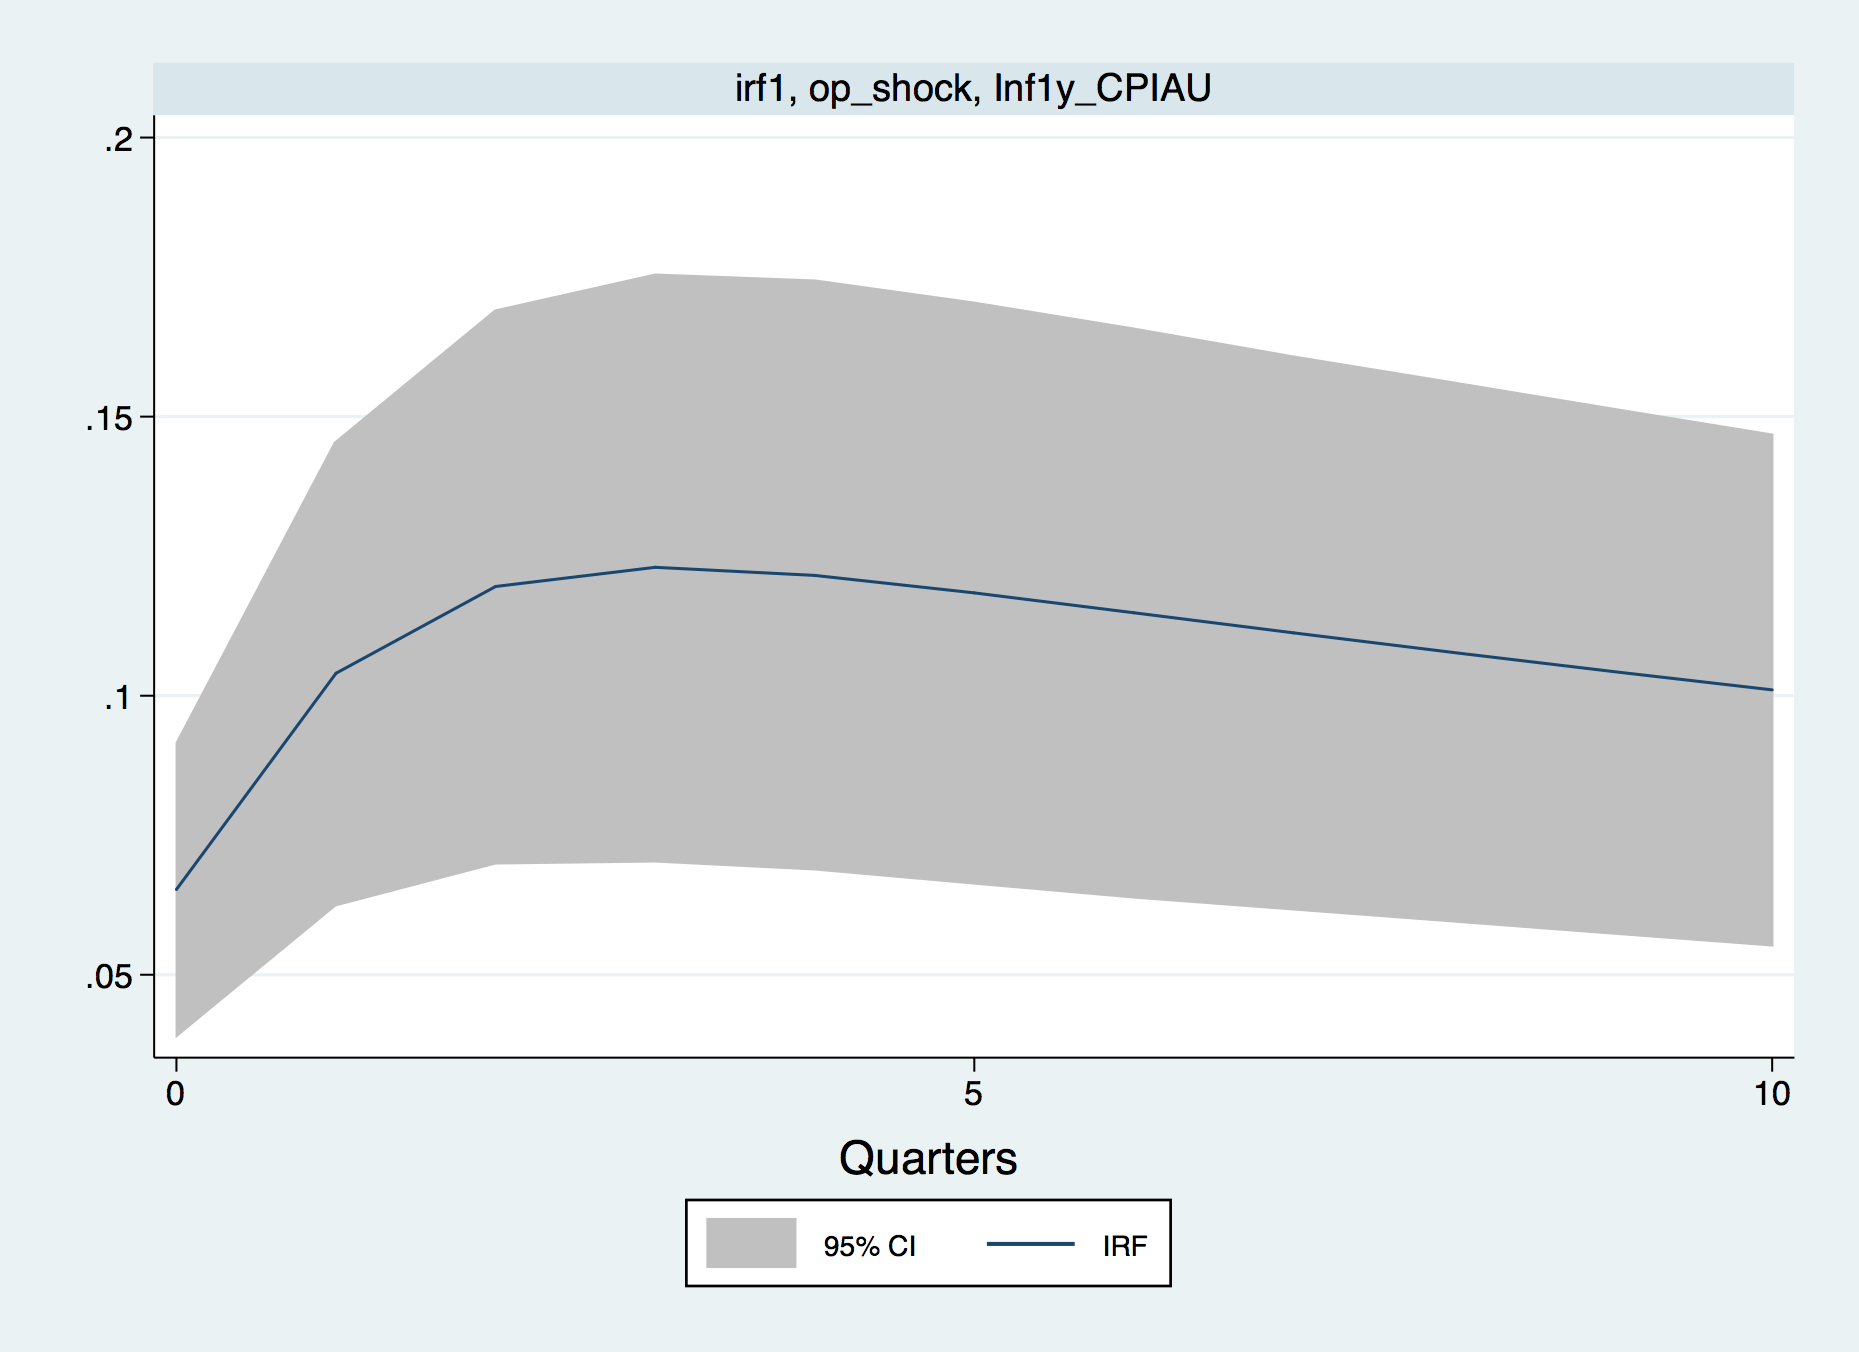
\includegraphics[width=4.5cm,height=3.5cm]{figures/CPIAU_ashocks_nmpM.png}
			\smallskip
			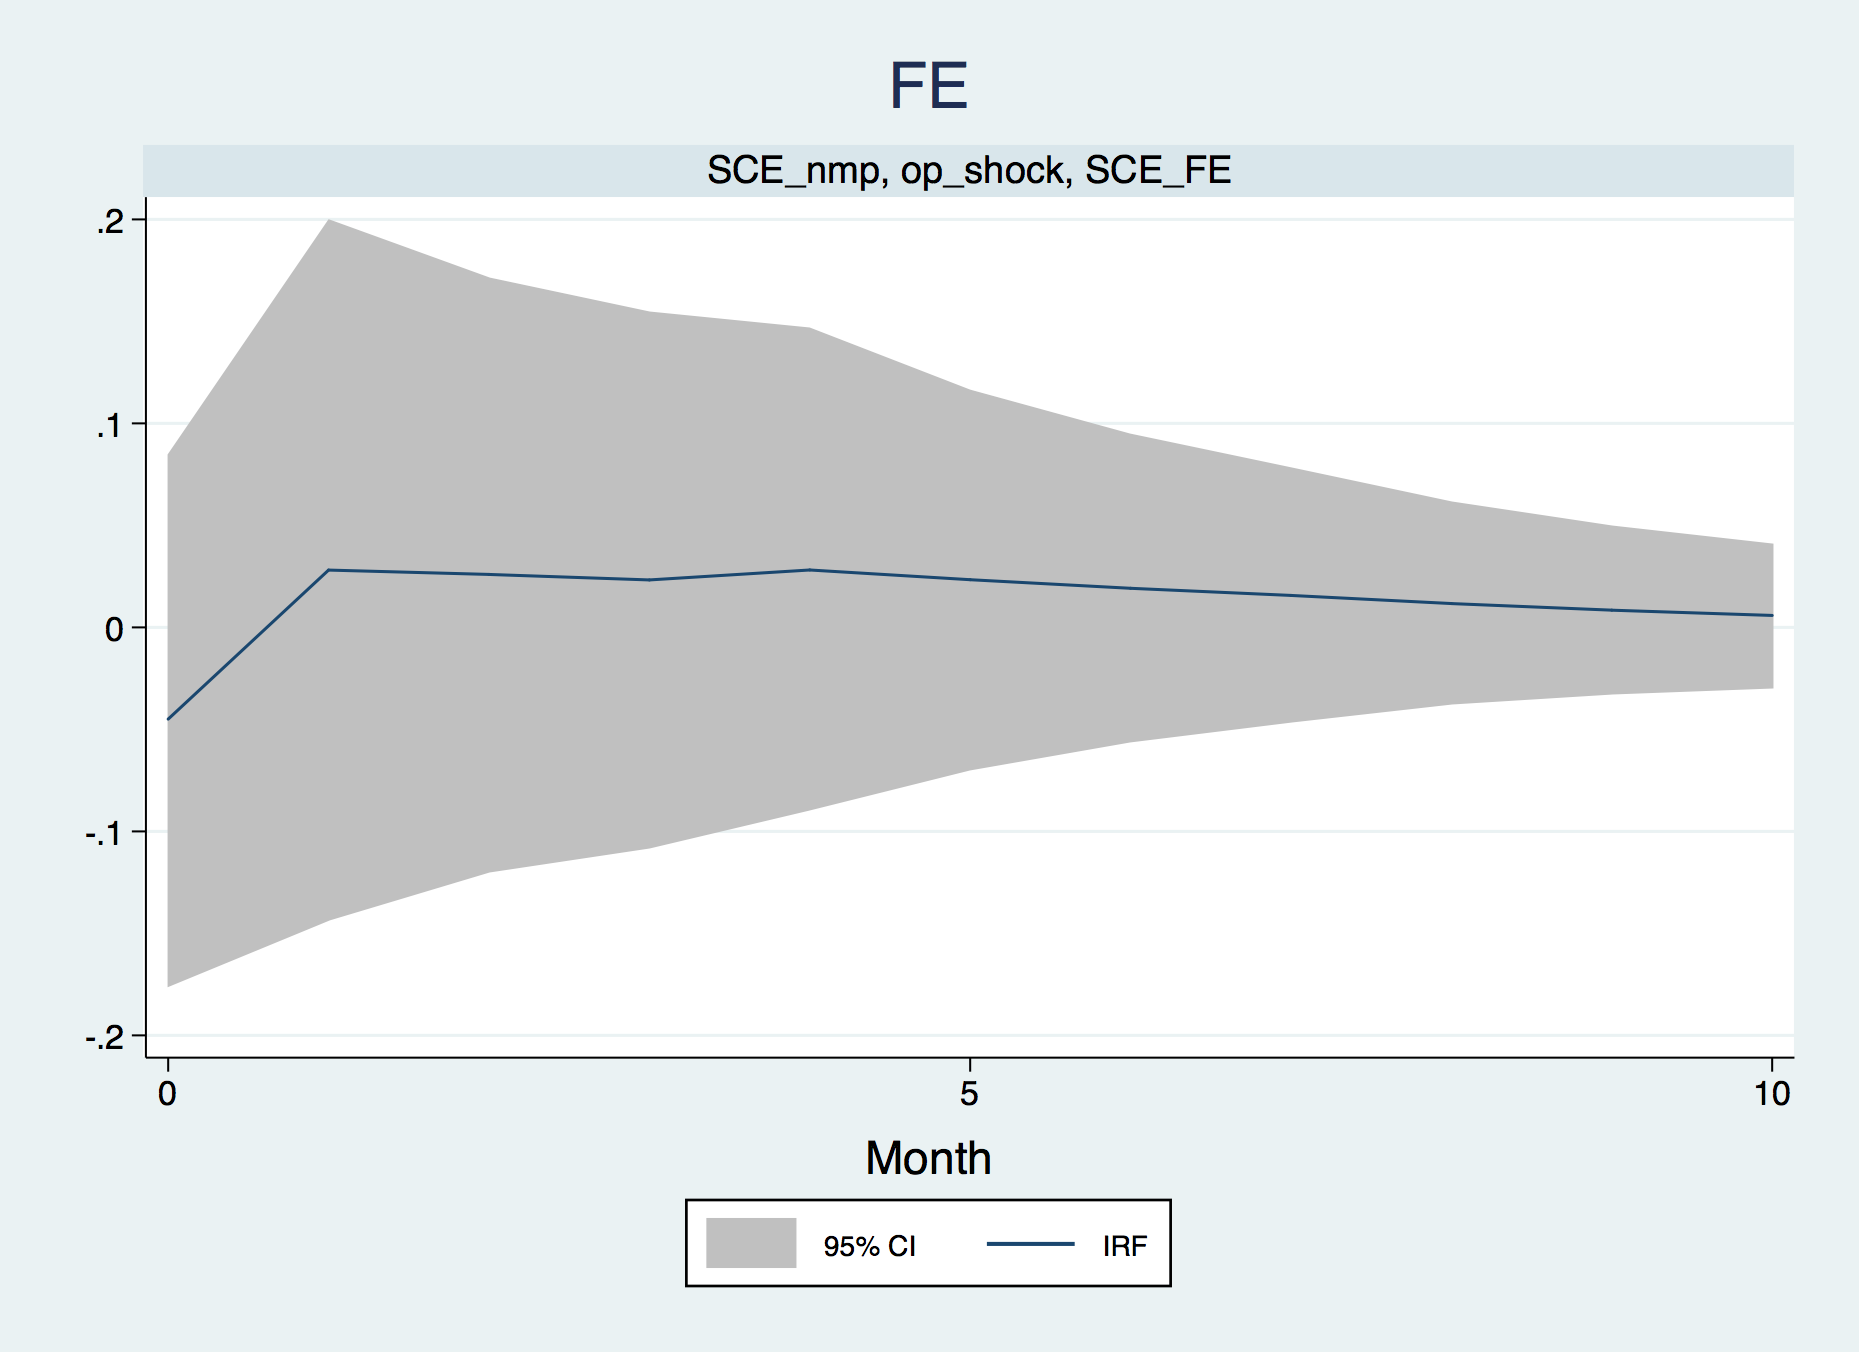
\includegraphics[width=4.5cm,height=3.5cm]{figures/SCEFE_ashocks_nmpM.png} 
			\smallskip
			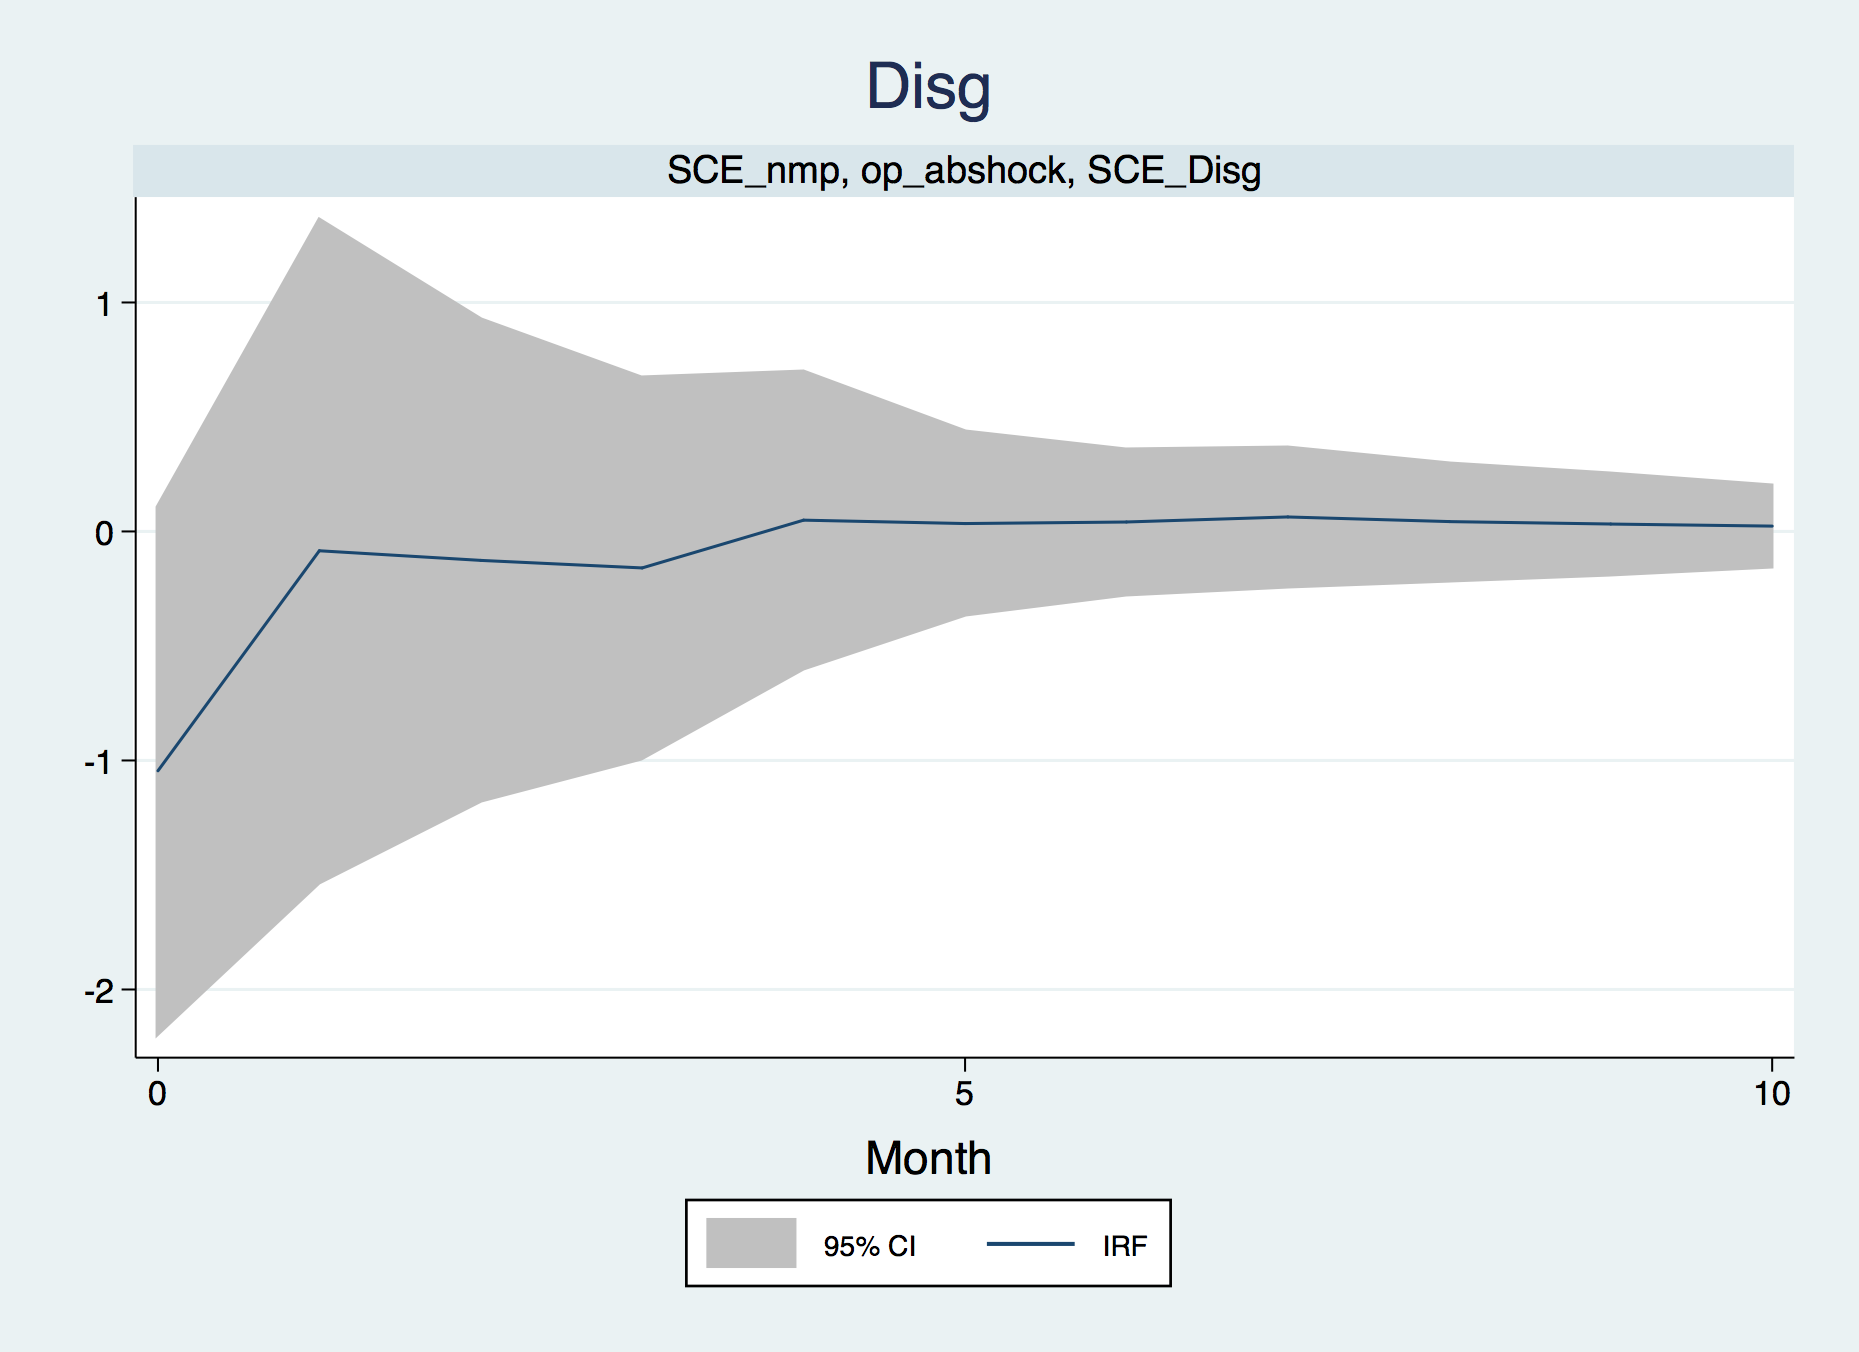
\includegraphics[width=4.5cm,height=3.5cm]{figures/SCEDisg_ab_ashocks_nmpM.png}
			\smallskip
			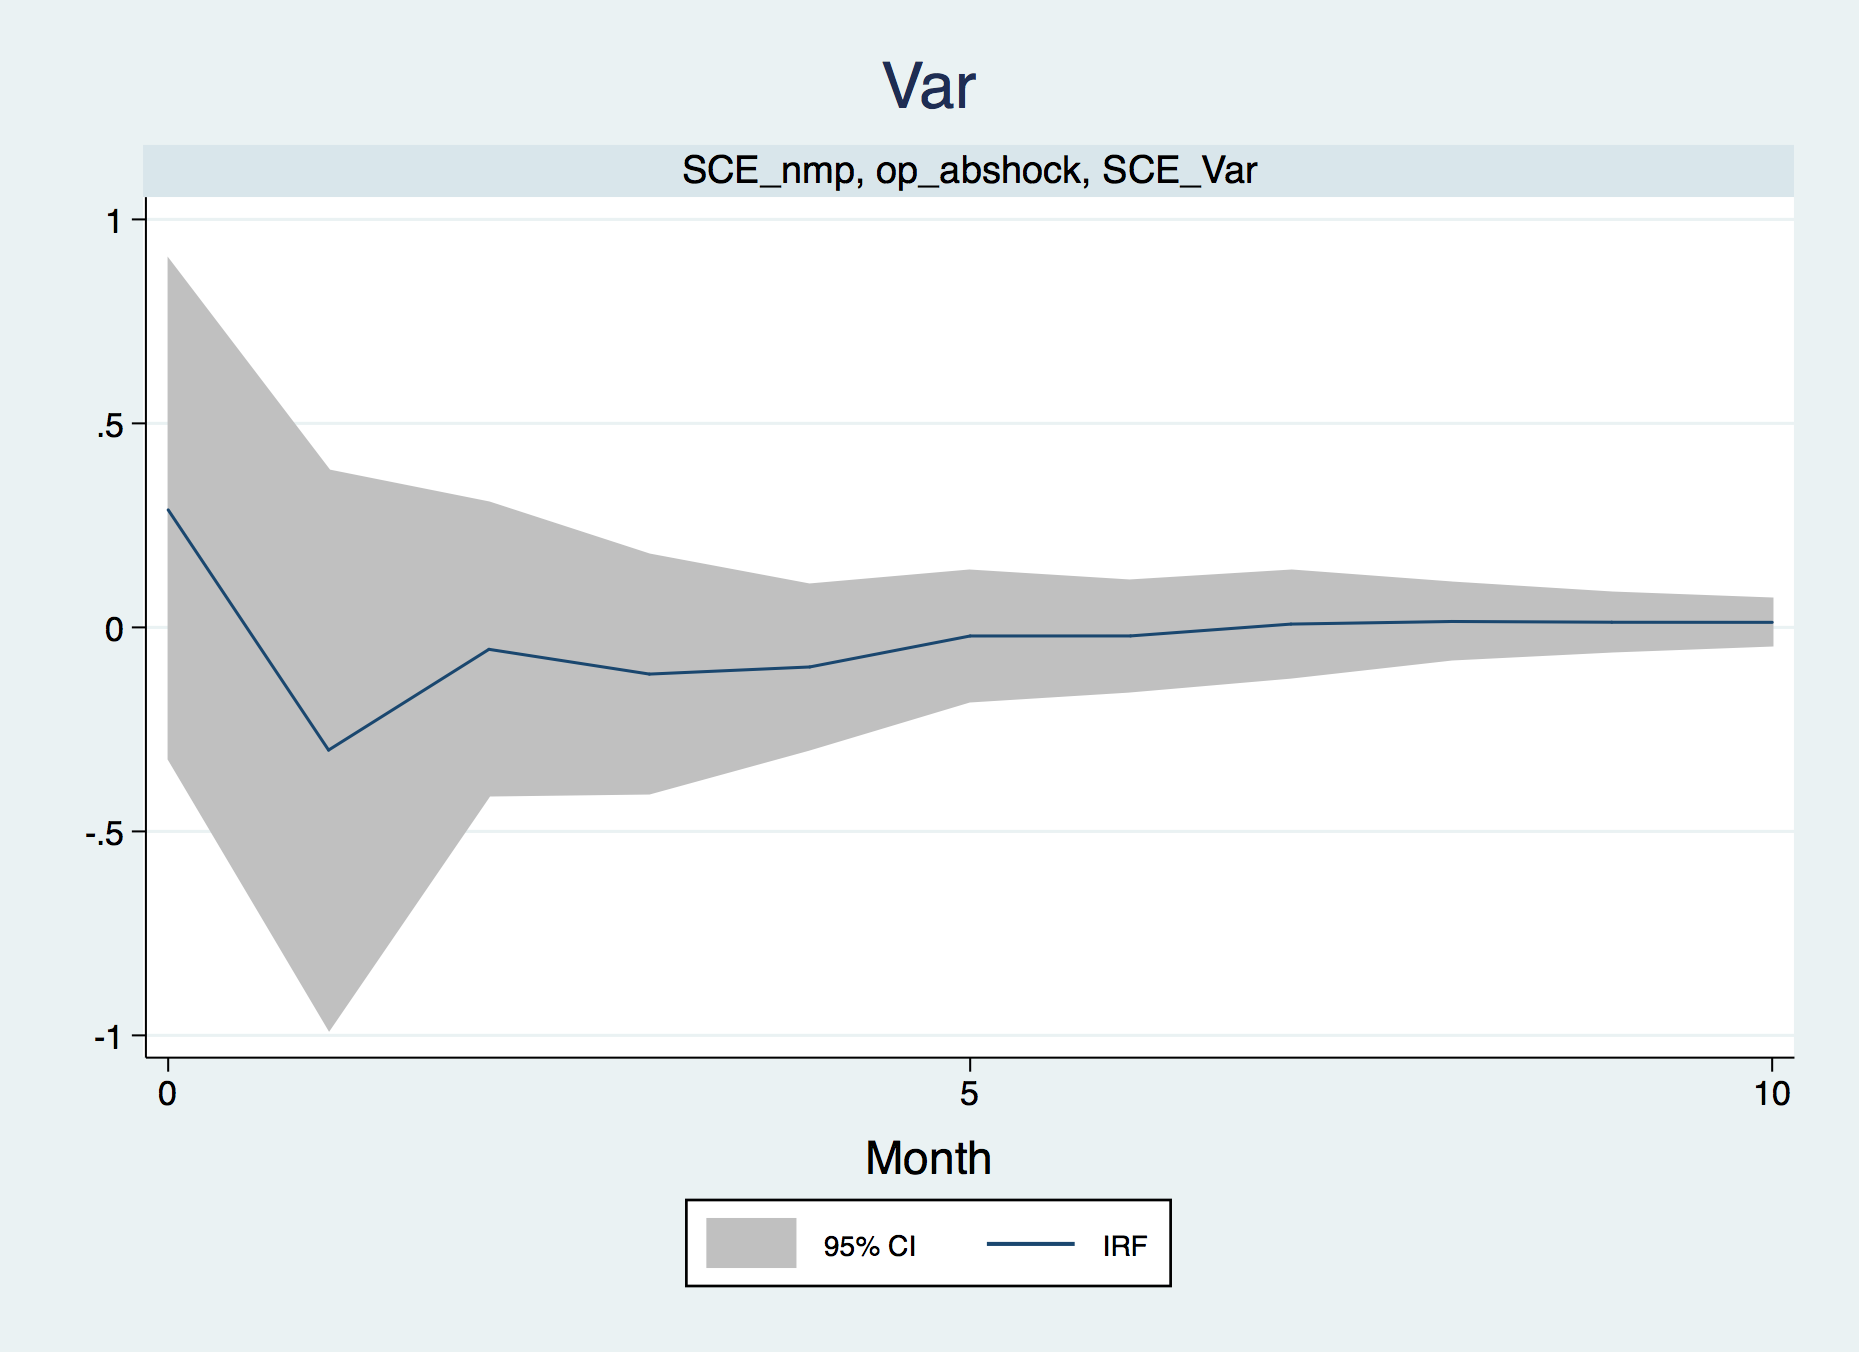
\includegraphics[width=4.5cm,height=3.5cm]{figures/SCEVar_ab_ashocks_nmpM.png}
		\end{subfigure}
		\hfill
		\begin{subfigure}[b]{0.65\textwidth}
			\centering
			\caption{Monetary Policy Shocks}
			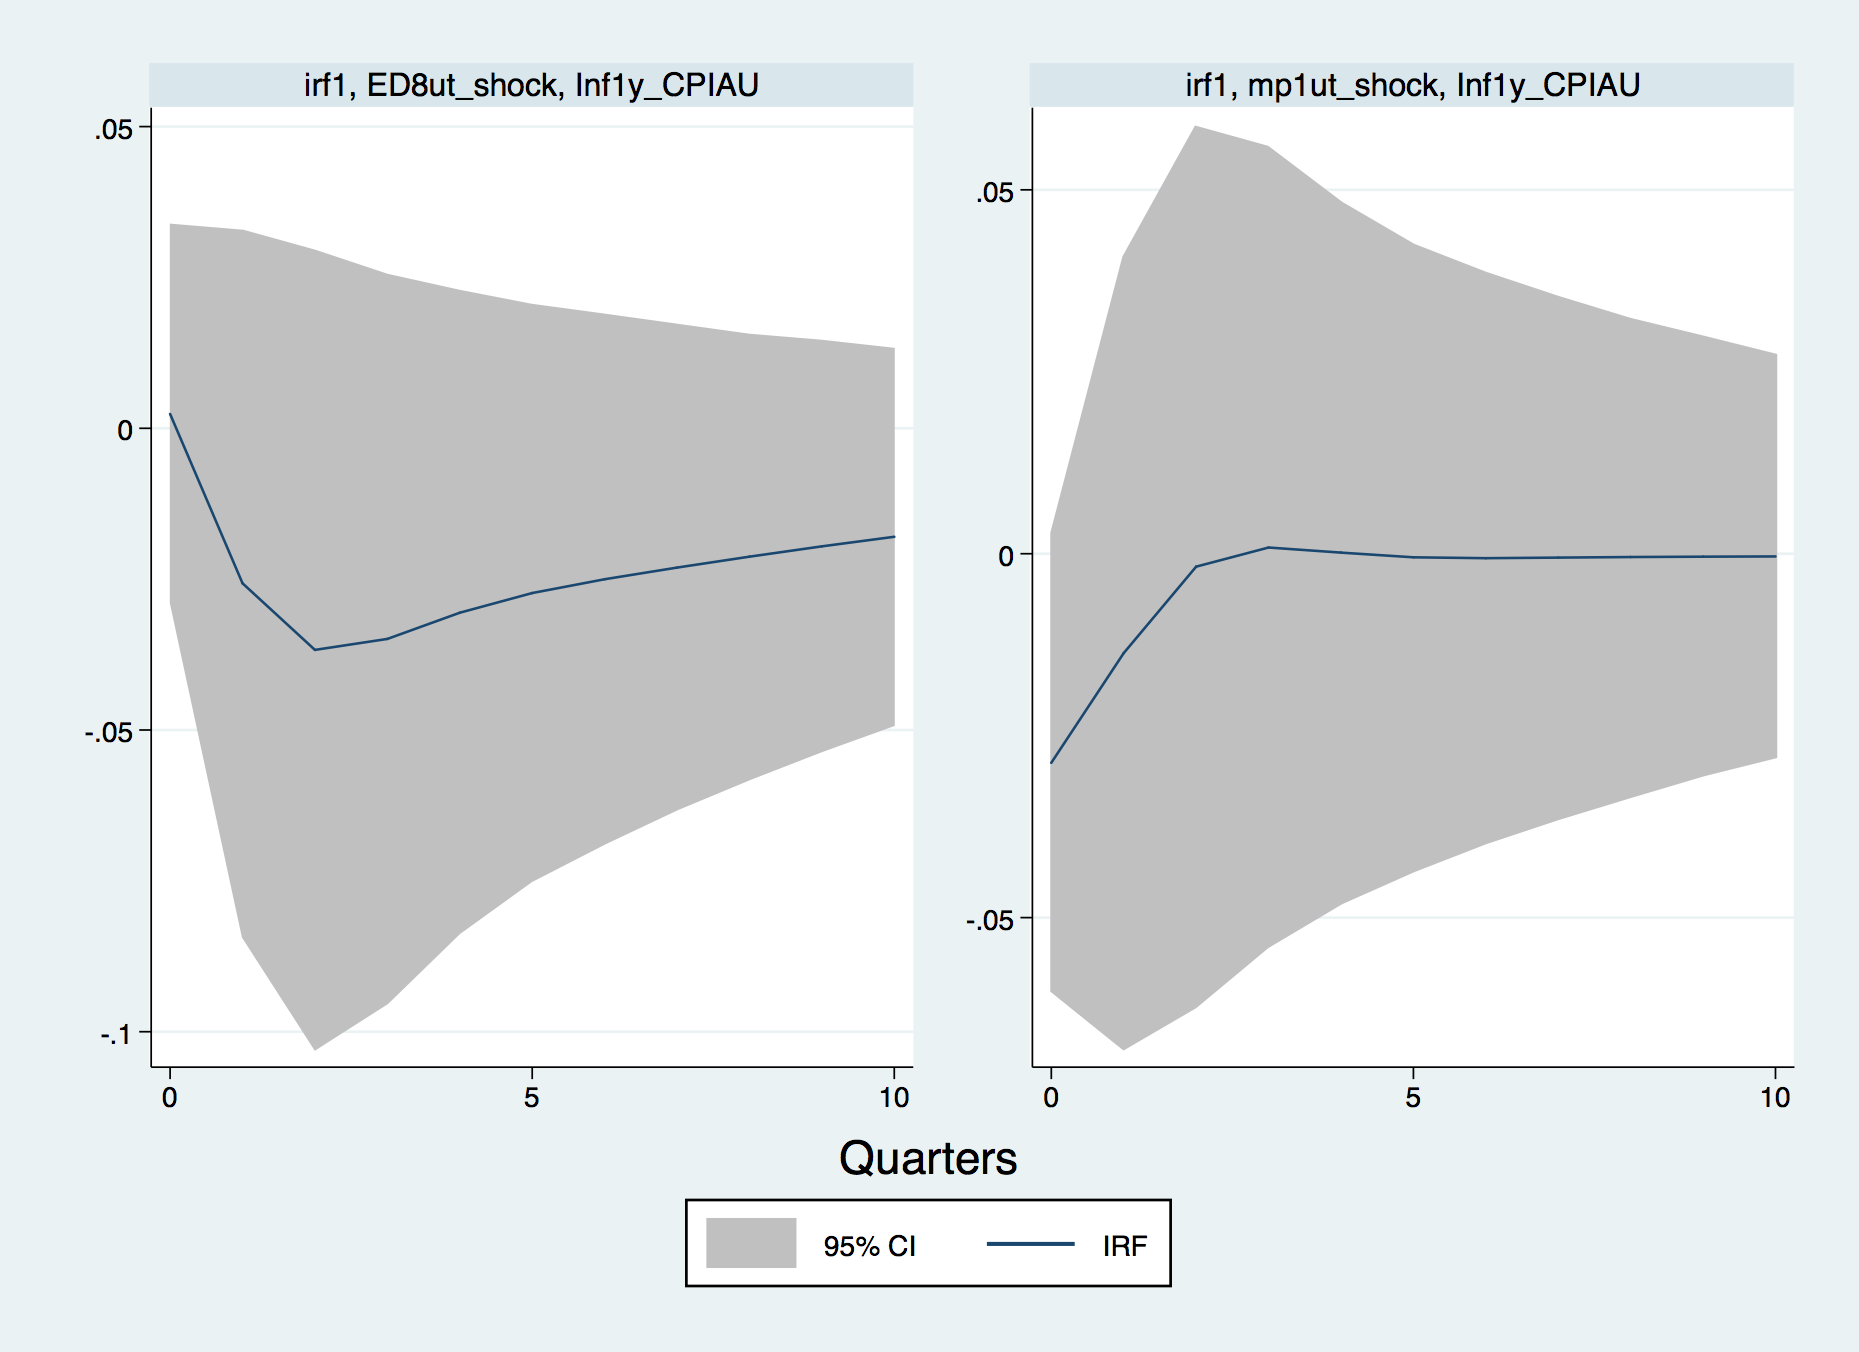
\includegraphics[width=9cm,height=3.5cm]{figures/CPIAU_ashocksM.png} 
			\smallskip
			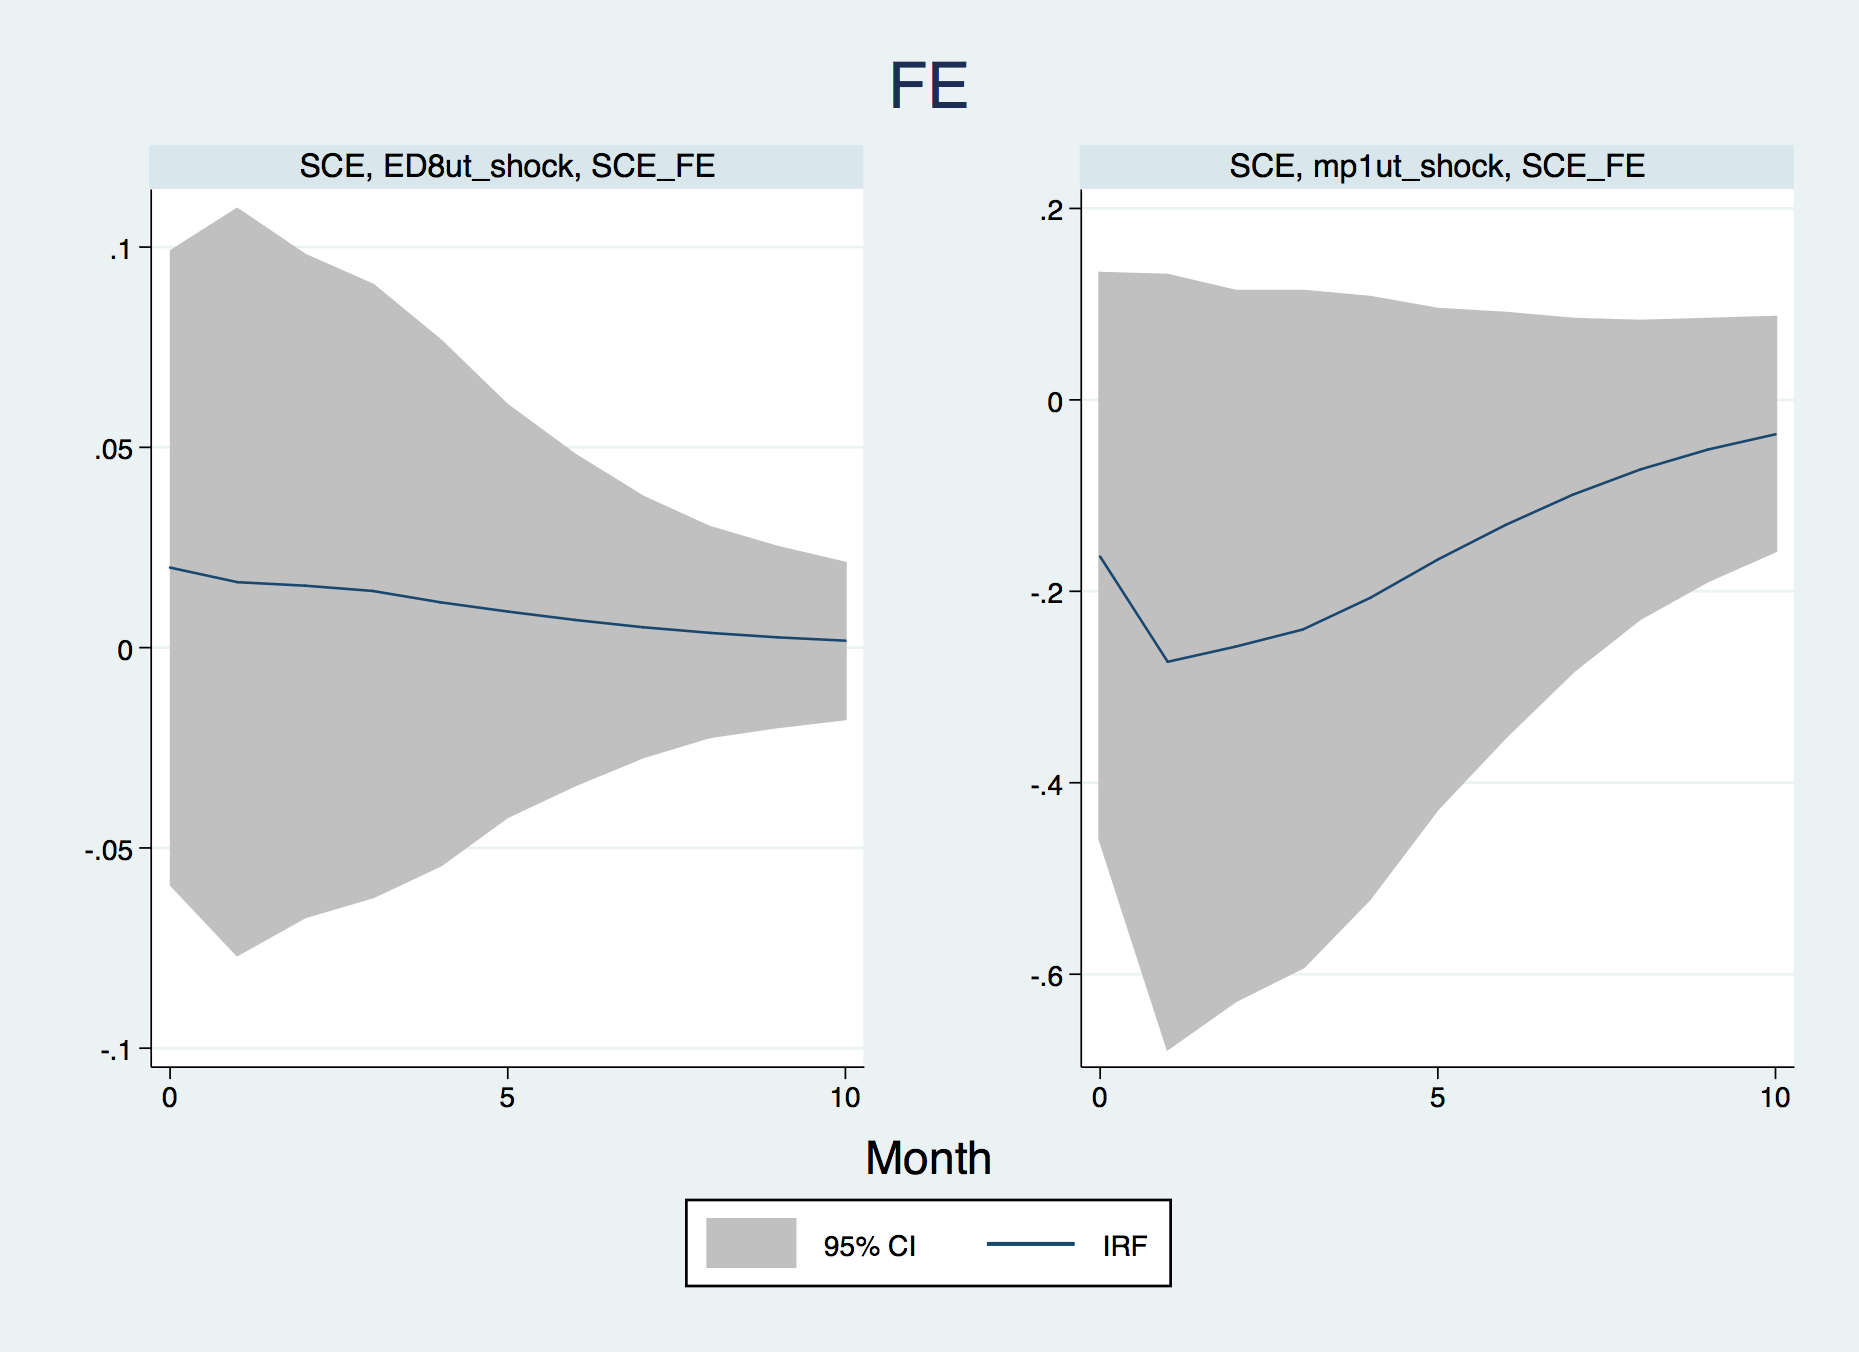
\includegraphics[width=9cm,height=3.5cm]{figures/SCEFE_ashocksM.png} 
			\smallskip
			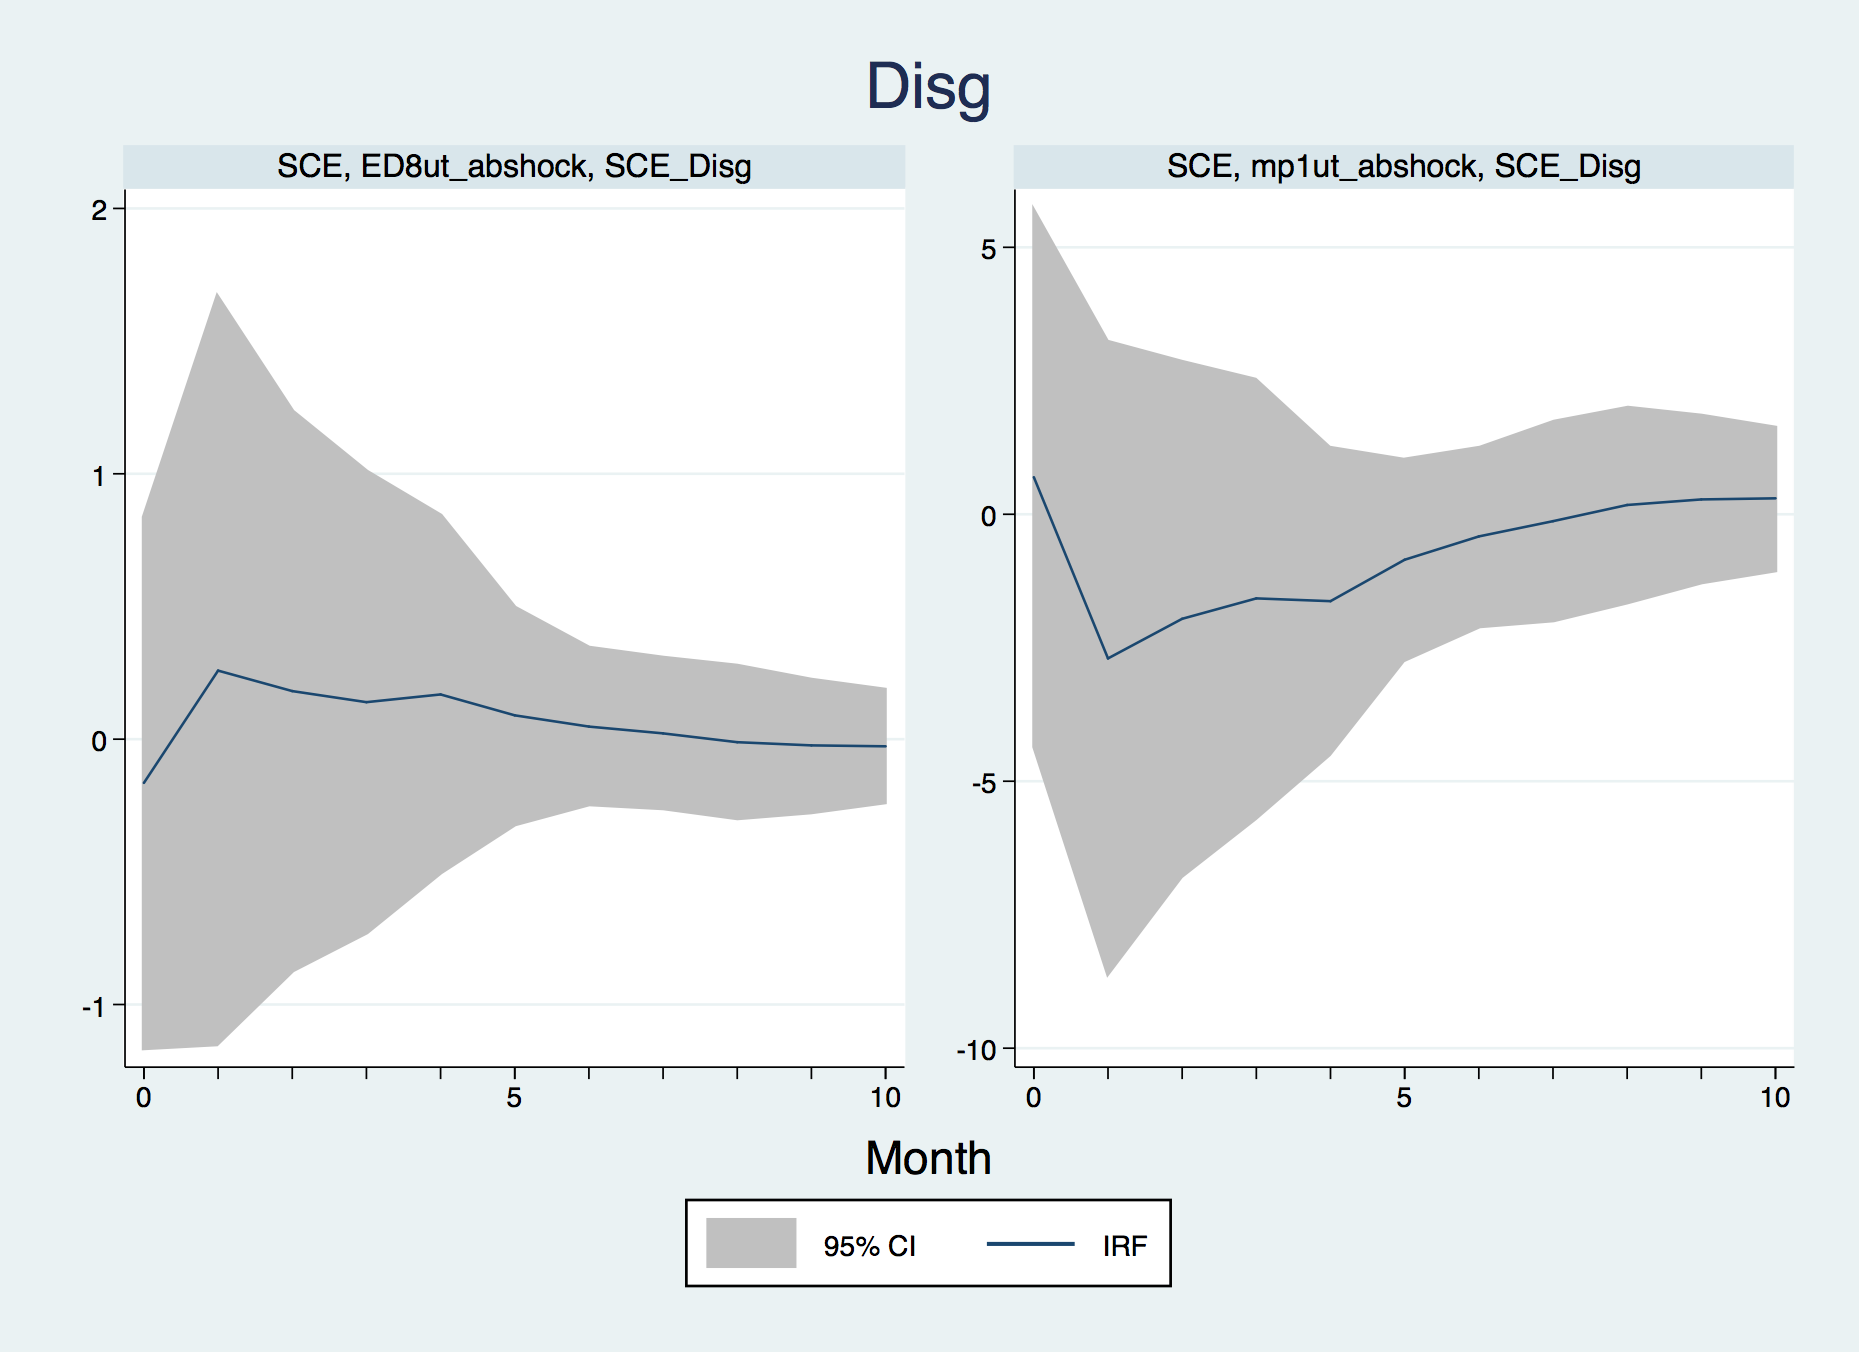
\includegraphics[width=9cm,height=3.5cm]{figures/SCEDisg_ab_ashocksM.png} 
			\smallskip 
			\includegraphics[width=9cm,height=3.5cm]{figures/SCEVar_ab_ashocksM.png} 
		\end{subfigure}
		\caption{ Responses of Inflation and Household Forecast Moments: 2013-2019}
		\label{SCE_IR}
	\end{figure}
	
	
	\subsection{Discussion of the results and next step}
	
	This section presents one major additional insight in addition to \cite{coibion2012can}: expectation rigidity is dependent on the type of shock. In particular, professional forecasters are slow in digesting oil and technology shock to resolve disagreements and reduce forecast error while react to monetary policy shocks relatively more efficient. This is the easiest seen in the non-response or instantaneous response if any of forecast error and disagreements to monetary policy shocks. The similar can be said for households, in contrast, for oil price shock instead of monetary policy shocks.
	
	Shock-dependent rigidity is not a default feature in the benchmark rigidity models such as SE and NI, i.e. $\omega_t$ in Equation \ref{AR_process}. It is true that the distinction of public and private signals within NI provides one possibility of reconciling difference in response to shocks.  If we interpret different ``shocks'' considered here as noisy signals instead of shocks to fundamental variable as defined in Equation \ref{AR_process}, then the difference across ``shocks'' in their degree of publicity may account for the difference in rigidity.  But this implicitly implies redefining the  framework presented in this paper. 
	
	Moreover, the finding that average uncertainty of fixing horizon by forecasters and households do not react to all the shocks is consistent with the current framework although it does not differentiate rigidity models from FIRE benchmark.  
	
	Efficient revision implies  uncertainty drop as much as the volatility of the realized shock as one approach the terminate date. Given the volatility of shocks are different, this provides the possibility of identifying rigidity by directly comparing the observed revision in uncertainty with the externally identified volatility of various shocks. This will be the next step of the analysis.  
	
	\section{Conclusion}\label{Conclusion}
	
	In summary, three major conclusions can be drawn from this paper.  First, full information rational expectation implicitly assumes agents share the common information and agree on the model that generates the data. Therefore, agents do not only agree on the mean forecast of a macroeconomic variable but also share the same degree of uncertainty. The empirical dispersion of individual uncertainty in future inflation seems to be inconsistent with this simple prediction. 
	
	Second, rigidity of expectation from either inattention or under-reaction due to noisiness of the signals implies agents do not revise forecasts as efficiently as they do in FIRE in the face of new information. This can be seen from both a sluggish pattern of forecast revision or uncertainty reduction across different vintages of the forecast. A weaker test of this spirit uses the changes in mean forecasts and uncertainty with fixed forecasting horizon. These tests support rigidity models in addition to other null hypotheses tests of rational expectation including unbiasedness,  non-serial-correlation of forecast errors, etc.
	
	Lastly, the directly estimated response of households and professional forecasters' expectation to shocks to inflation suggest that rigidity differs across the shocks. In particular, professional forecasters are more responsive to monetary policy shocks and households are more responsive to oil price shocks. This motivates a next-step analysis of how much resolution of uncertainty can be attributed to the volatility of various shocks. This shows the use of uncertainty.
	
	So far, the dynamics of moments are separately estimated for each moment. Therefore, as a natural extension of the current analysis, one can undertake a generalized method of moment (GMM) estimation that simultaneously utilizes multi-moment restrictions to recover a better estimate of the rigidity parameters.  This will provide a better parameter that can be used in structural macro models that build in rigidity of expectations. 
	
	\bibliographystyle{apalike}
	\bibliography{TestingExpectationTheories}
	
\end{document}
